\documentclass[12pt,oneside]{book}
\usepackage[a4paper, margin=1in, headheight=15pt]{geometry}
\usepackage{setspace}
\usepackage{graphicx}
\usepackage[export]{adjustbox}
\usepackage{titlesec}
\usepackage{array}
\usepackage{enumitem}
\usepackage{multirow}
\usepackage{booktabs}
\usepackage{longtable}
\usepackage{tabularx}
\usepackage{float}
\usepackage{url}
\usepackage{rotating}
\usepackage{fancyhdr}
\renewcommand{\arraystretch}{1.2}
\renewcommand{\bibname}{References}

\setlength{\intextsep}{5pt}
% Long-table captions may use the full text width (no hyphenated wraps).
\setlength{\LTcapwidth}{\textwidth}
% Contents lists: a wider page-number column, so a title that fills the
% line still keeps a gap before its page number.
\makeatletter
\renewcommand{\@pnumwidth}{2.2em}
\renewcommand{\@tocrmarg}{3.2em}
\makeatother

\makeatletter
\def\@makechapterhead#1{%
  {\parindent \z@ \raggedright \normalfont
    \ifnum \c@secnumdepth >\m@ne
        \huge\bfseries \@chapapp\space \thechapter
        \par\nobreak
        \vskip 10\p@
    \fi
    \interlinepenalty\@M
    \Huge \bfseries #1\par\nobreak
    \vskip 10\p@
  }}
\def\@makeschapterhead#1{%
  {\parindent \z@ \raggedright
    \normalfont
    \interlinepenalty\@M
    \Huge \bfseries  #1\par\nobreak
    \vskip 10\p@
  }}
\makeatother

\titlespacing\section{0pt}{12pt plus 4pt minus 2pt}{6pt plus 2pt minus 2pt}
\titlespacing\subsection{0pt}{10pt plus 3pt minus 2pt}{4pt plus 2pt minus 1pt}
\titlespacing\subsubsection{0pt}{8pt plus 2pt minus 2pt}{0.5em}

\titleformat{\subsubsection}[runin]
  {\normalfont\normalsize\bfseries}{\thesubsubsection}{1em}{}[.]

\newcommand\tab[1][0.75cm]{\hspace*{#1}}
\setcounter{tocdepth}{2}
\setcounter{secnumdepth}{3}

\newcommand{\hiddensubsection}[1]{
    \stepcounter{subsection}
    \subsection*{\arabic{chapter}.\arabic{section}.\arabic{subsection}\hspace{1em}{#1}}
}

\newcommand{\hiddensection}[1]{
    \stepcounter{subsection}
    \subsection*{\arabic{chapter}.\arabic{section}\hspace{1em}{#1}}
}

\newcolumntype{C}[1]{>{\centering\arraybackslash}m{#1}}
\newcolumntype{P}[1]{>{\raggedright\arraybackslash}p{#1}}

\usepackage{amssymb}
\usepackage{pifont}
\newcommand{\cmark}{\ding{51}}%
\newcommand{\xmark}{\ding{55}}%

% \DiagramBarrier, a local copy of the placeins \FloatBarrier (the package is
% not loaded), flushes pending figures before the next paragraph, so each
% paragraph in Chapters 5 and 6 is followed by its own figures.
\makeatletter
\newcommand{\DiagramBarrier}{\par\begingroup\let\@elt\relax
  \edef\@tempa{\@botlist\@deferlist\@dbldeferlist}%
  \ifx\@tempa\@empty\else\clearpage\fi\endgroup}
\makeatother

\begin{document}

% Front matter: roman numbers at the bottom centre. The title, certificate
% and declaration pages are counted but print no number.
\pagenumbering{roman}
\pagestyle{plain}
\thispagestyle{empty}
\onehalfspacing

\begin{center}
\vspace*{12pt}

\includegraphics[width=2in]{Figures/Logo.jpg}

\vspace{1cm}

{\Huge\textbf{AI-Driven Lab Exam Monitoring\\
and Management System}\par}

\vspace{5cm}

\normalsize
\textbf{Zain Ali Mehmood (2280133)}\\
\textbf{Muhammad Haider Ali (2280354)}\\
\textbf{Roshaan Ali Shah (2280327)}

\vspace{2cm}

\textbf{Supervised by: Ms.~Zainab Iftikhar Chaudhary}

\vspace*{\fill}
\textbf{In partial fulfillment of the requirements for the degree}\\
\textbf{Bachelor of Science (Software Engineering)}\\
\textbf{Shaheed Zulfikar Ali Bhutto Institute of Science and Technology}\\
\textbf{Islamabad, Pakistan}

\vspace{10pt}
\textbf{Spring, 2026}
\end{center}

\singlespacing
\newpage
\thispagestyle{empty}

\begin{center}
\vspace*{0.8cm}

{\bfseries\fontsize{20}{24}\selectfont 
AI-Driven Lab Exam Monitoring and\\
Management System\par}

\vspace{0.8cm}

{\bfseries\itshape\fontsize{16}{18}\selectfont By\par}

\vspace{0.5cm}

{\bfseries\itshape\fontsize{14}{16}\selectfont
Zain Ali Mehmood (2280133)\\
Muhammad Haider Ali (2280354)\\
Roshaan Ali Shah (2280327)\par}

\vspace{0.8cm}

{\bfseries\fontsize{22}{26}\selectfont CERTIFICATE\par}

\end{center}

\vspace{0.6cm}

\begin{center}
{\bfseries\fontsize{11}{14}\selectfont
A THESIS SUBMITTED IN PARTIAL FULFILLMENT OF THE REQUIREMENTS FOR THE DEGREE OF BACHELOR OF SCIENCE IN SOFTWARE ENGINEERING (BSSE).\par}
\end{center}

\vspace{0.6cm}

{\fontsize{12.5}{14}\selectfont
It is to certify that the above students' thesis has been completed to my satisfaction and, to my belief, its standard is appropriate for submission for evaluation. I have also carried out a plagiarism test of this thesis using HEC-prescribed software and found a similarity index of \underline{\hspace{1.5cm}}\%, which is within the permissible limit set by the HEC for the BSSE degree thesis. I have also found the thesis to be in the format recognised by SZABIST for the BSSE thesis.
}

\vspace{1.5cm}

\noindent
\begin{minipage}{0.48\textwidth}
\centering
\rule{6cm}{0.4pt}\\[4pt]
(Supervisor)\\
Ms. Zainab Iftikhar
\end{minipage}
\hfill
\begin{minipage}{0.48\textwidth}
\centering
\rule{6cm}{0.4pt}\\[4pt]
(FYP Committee Head)\\
Mr. Fakhar-ul-Islam
\end{minipage}

\vspace{1.5cm}

\noindent
\begin{minipage}{0.48\textwidth}
\centering
\rule{6cm}{0.4pt}\\[4pt]
(Program Manager BSSE)\\
Mr. Sheikh Abdul Wahab
\end{minipage}
\hfill
\begin{minipage}{0.48\textwidth}
\centering
Date: \rule{4.5cm}{0.4pt}
\end{minipage}

\vfill

\begin{center}
\normalsize\textbf{Department of Computer Science, Shaheed Zulfikar Ali Bhutto Institute of Science and Technology, Islamabad Campus}\\
\vspace{6pt}
\normalsize\textbf{Spring, 2026}
\end{center}
\newpage
\thispagestyle{empty}
\begin{center}
    {\Huge\textbf{DECLARATION}}
\end{center}
\vspace{1cm}

\begin{onehalfspacing}
We, Zain Ali Mehmood (2280133), Muhammad Haider Ali (2280354) and Roshaan Ali Shah (2280327), students of the Bachelor of Science in Software Engineering at Shaheed Zulfikar Ali Bhutto Institute of Science and Technology, Islamabad, declare that the project titled ``AI-Driven Lab Exam Monitoring and Management System'' is our own work.

This project has not been submitted before for any degree or examination at any other university or institute. We have acknowledged all sources of information and data used in this document.\par
\end{onehalfspacing}

\vspace{2cm}

\noindent
\begin{minipage}{0.45\textwidth}
\centering
\rule{6cm}{0.4pt}\\[4pt]
Zain Ali Mehmood\\
(2280133)
\end{minipage}
\hfill
\begin{minipage}{0.45\textwidth}
\centering
\rule{6cm}{0.4pt}\\[4pt]
Muhammad Haider Ali\\
(2280354)
\end{minipage}

\vspace{1.8cm}

\begin{center}
\begin{minipage}{0.45\textwidth}
\centering
\rule{6cm}{0.4pt}\\[4pt]
Roshaan Ali Shah\\
(2280327)
\end{minipage}
\end{center}

\newpage
\thispagestyle{empty}
\chapter*{\centering Project Overview}
\addcontentsline{toc}{chapter}{Project Overview}

A practical lab exam is hard to supervise. One or two invigilators watch 30 to 40 screens, attendance is marked on paper, and code is collected on USB drives. SmartExam, the system built for our registered project ``AI-Driven Lab Exam Monitoring and Management System'', replaces this with three parts: a Windows Presentation Foundation (WPF) client on each lab PC, a React web panel for staff and students, and an ASP.NET Core 9 API backed by PostgreSQL on Neon.

Teachers create exams with multiple-choice (MCQ), coding and theory questions, set eligibility from imported attendance and assign each student a workstation. A student can log in only from the workstation bound to the account by its hardware ID. After a readiness check, the client locks the PC: fullscreen window, blocked shortcuts, clipboard guard and a check for unapproved programs. It reports heartbeats, focus and process events, screenshots and, when the exam requires it, webcam checks (camera covered or frozen, no face or several faces, head turned away, phone in view); no face is matched to an identity. A rule-based classifier rates each student, and invigilators follow every seat on a live SignalR dashboard, from which they can warn a student, extend time, unlock the PC or force a submission. Each edit goes to an encrypted local backup within a second and to the server within 10 seconds. Practice exams let students rehearse without affecting their results.

After each submission, C and C++ answers run against the teacher's test cases in an isolated Docker container where available (otherwise with a local compiler that is not isolated), theory answers get a TF-IDF similarity score, and k-gram winnowing flags similar code. The teacher reviews every suggested mark. Security-relevant actions are kept in a hash-chained, tamper-evident audit log, and teachers export PDF reports, an Excel workbook and an evidence ZIP. We built the system in eight four-week Agile sprints. Automated unit, integration, API and browser tests cover all twelve modules (Chapter~7); checks that need a real lab PC, such as the webcam, USB and 40-client load checks, are still pending.

\newpage
\thispagestyle{empty}
\chapter*{\centering Dedication}
\addcontentsline{toc}{chapter}{Dedication}
%\centerline{\textbf{\LARGE DEDICATION}}
\par\bigskip
Firstly, we dedicate this project to Allah Almighty, whose blessings, mercy, and guidance made this effort possible. We also dedicate this work to our Holy Prophet Muhammad (Peace Be Upon Him), whose teachings remain a source of inspiration in all aspects of life. Finally, we dedicate this project to our beloved parents, respected teachers, supervisor, and supportive friends whose prayers, encouragement, and sacrifices have helped us continue our academic journey with determination and hope.

\newpage
\thispagestyle{empty}

\chapter*{\centering Acknowledgements}
\addcontentsline{toc}{chapter}{Acknowledgements}
\par\bigskip
This Final Year Project has been completed in partial fulfillment of the requirements for the degree of Bachelor of Science in Software Engineering. We sincerely thank our supervisor, Ms. Zainab Iftikhar Chaudhary, for her guidance, encouragement, and constructive feedback throughout the development of this project. We are also grateful to the faculty members of the Department of Computer Science, SZABIST Islamabad, and our families and friends for their continuous support, motivation, and prayers during the planning, implementation, and report-writing phases of this work.

\vspace{2cm}

\noindent
\begin{minipage}{0.45\textwidth}
\centering
\rule{6cm}{0.4pt}\\[4pt]
Zain Ali Mehmood\\
(2280133)
\end{minipage}
\hfill
\begin{minipage}{0.45\textwidth}
\centering
\rule{6cm}{0.4pt}\\[4pt]
Muhammad Haider Ali\\
(2280354)
\end{minipage}

\vspace{1.8cm}

\begin{center}
\begin{minipage}{0.45\textwidth}
\centering
\rule{6cm}{0.4pt}\\[4pt]
Roshaan Ali Shah\\
(2280327)
\end{minipage}
\end{center}

\chapter*{Revision History}
\addcontentsline{toc}{chapter}{Revision History}

\begin{center}
\scriptsize
\setlength{\tabcolsep}{3pt}
\renewcommand{\arraystretch}{1.1}
\begin{tabularx}{\textwidth}{|l|l|l|>{\raggedright\arraybackslash}X|c|}
\hline
\textbf{Compiled By} & \textbf{Checked By} & \textbf{Date} & \textbf{Reason for Change} & \textbf{Version} \\
\hline
All members & Ms. Zainab Iftikhar Chaudhary & 24 Feb 2026 & FYP-I proposal submitted & 0.1 \\
\hline
Muhammad Haider Ali & Ms. Zainab Iftikhar Chaudhary & 10 Mar 2026 & Chapter 1 drafted from the proposal & 1.0 \\
\hline
Roshaan Ali Shah & Ms. Zainab Iftikhar Chaudhary & 16 Mar 2026 & Objectives (Section 1.3) added & 1.1 \\
\hline
Zain Ali Mehmood & Ms. Zainab Iftikhar Chaudhary & 22 Mar 2026 & Intended users (Section 1.7) added & 1.2 \\
\hline
Muhammad Haider Ali & Ms. Zainab Iftikhar Chaudhary & 28 Mar 2026 & SRS introduction (Section 2.1) & 1.3 \\
\hline
Roshaan Ali Shah & Ms. Zainab Iftikhar Chaudhary & 04 Apr 2026 & Chapter 3 project plan drafted & 1.4 \\
\hline
Zain Ali Mehmood & Ms. Zainab Iftikhar Chaudhary & 10 Apr 2026 & Management plan (Section 3.2) & 1.5 \\
\hline
Muhammad Haider Ali & Ms. Zainab Iftikhar Chaudhary & 15 Apr 2026 & Chapters 1--3 reviewed and refined & 1.6 \\
\hline
All members & Ms. Zainab Iftikhar Chaudhary & 18 Jun 2026 & FYP-I report submitted & 1.7 \\
\hline
Roshaan Ali Shah & Ms. Zainab Iftikhar Chaudhary & 05 Oct 2026 & Chapter 4 matched to the code & 1.8 \\
\hline
Zain Ali Mehmood & Ms. Zainab Iftikhar Chaudhary & 10 Oct 2026 & Chapter 5 design diagrams revised & 1.9 \\
\hline
Muhammad Haider Ali & Ms. Zainab Iftikhar Chaudhary & 15 Oct 2026 & Chapter 6 UI and tables revised & 2.0 \\
\hline
Roshaan Ali Shah & Ms. Zainab Iftikhar Chaudhary & 20 Oct 2026 & Chapter 7 test plan drafted & 2.1 \\
\hline
Muhammad Haider Ali & Ms. Zainab Iftikhar Chaudhary & 21 Oct 2026 & Module 12 tests and test run & 2.2 \\
\hline
Muhammad Haider Ali & Ms. Zainab Iftikhar Chaudhary & 26 Oct 2026 & Full review; final test run & 2.3 \\
\hline
Muhammad Haider Ali & Ms. Zainab Iftikhar Chaudhary & 27 Oct 2026 & Template sections added & 2.4 \\
\hline
\end{tabularx}
\end{center}

\tableofcontents

% \clearpage first, so that each entry records the page where its list starts.
\clearpage
\addcontentsline{toc}{chapter}{List of Figures}
\listoffigures

\clearpage
\addcontentsline{toc}{chapter}{List of Tables}
\listoftables


% Main matter: arabic numbers from 1, at the top right of every page.
\clearpage
\pagenumbering{arabic}
% Space between paragraphs from here on only, so the contents lists keep
% their tight spacing. Table and float cells reset it to zero.
\setlength{\parskip}{6pt plus 2pt minus 1pt}
\fancypagestyle{plain}{%
  \fancyhf{}%
  \fancyhead[R]{\thepage}%
  \renewcommand{\headrulewidth}{0pt}%
  \renewcommand{\footrulewidth}{0pt}}
\pagestyle{plain}
\chapter{INTRODUCTION}
\label{chap:introduction}

This chapter introduces SmartExam. It states the product's purpose and scope, reviews existing tools, and sets out our objectives, the problem we address and the solution we propose. It ends with the intended market and users and the process model we followed.

\section{Product Purpose}
\label{sec:productpurpose}

Computer science and software engineering students are tested in practical lab exams. They write, compile and debug code on a real machine, which a multiple-choice paper cannot assess. In many departments these exams are still run by hand. The schedule is shared on WhatsApp, attendance is marked on a paper sheet, and students hand in their code by email or on a USB drive when time runs out. During the exam one or two invigilators walk between 30 and 40 machines. They cannot see every screen, and when they suspect cheating there is little record to check afterwards.

SmartExam is the system name of our registered project, the AI-Driven Lab Exam Monitoring and Management System, and it brings these steps together. Administrators manage users, roles, departments, courses, labs and workstations from a web panel. Teachers create exams with multiple-choice (MCQ), coding and theory questions, add test cases and list the applications students may use. Students log in on the Windows Presentation Foundation (WPF) client, which only works on their registered workstation. After a readiness check, the client locks the PC to the exam. Invigilators follow each seat on a live dashboard that shows focus changes, running processes, screenshots and warnings. As each student submits, the server grades coding answers against the test cases, scores theory answers and checks for plagiarism. The teacher reviews the suggested marks and can override any of them, and generates reports when needed. Students see their results on a web portal once the exam has ended.

Our aim is to make lab exams fair, supervised and auditable without adding staff to the room.

\section{Product Scope}

SmartExam covers a lab exam from set-up to final report. We drew the scope boundary \cite[ch.~5]{pmbok6} around the institution's own lab: exams on Windows PCs on campus, not at home. The WPF client on each workstation and the React web panel both call an ASP.NET Core 9 API that stores data in PostgreSQL on Neon. They use REST calls, over plain HTTP on the shipped localhost configuration and HTTPS behind a TLS endpoint in a lab deployment; the API itself does not enforce HTTPS. SignalR carries live updates between the API and the web dashboard. The desktop client uses REST only and receives invigilator warnings, extra time, unlocks and force-submits in the reply to its next heartbeat (every 10 s). The work is split into twelve modules:

\begin{itemize}[noitemsep]
\item M1 Authentication and Device Binding
\item M2 Pre-Exam Verification and Practice Exam
\item M3 Student Exam Dashboard
\item M4 Secure Exam Environment (lockdown)
\item M5 Live Monitoring Client Service
\item M6 Submission and Backup
\item M7 User and Role Management
\item M8 Exam Creation and Configuration
\item M9 Eligibility and Access Control
\item M10 Live Proctoring Dashboard
\item M11 AI-Assisted Evaluation
\item M12 Logs, Analytics and Audit Trail
\end{itemize}

Table~\ref{tab:Abbreviations} lists the abbreviations used in this report.

\begin{longtable}{cl>{\raggedright\arraybackslash}p{9.6cm}}
\caption{Abbreviations}
\label{tab:Abbreviations}\\
\hline
\textbf{Serial \#} & \textbf{Abbreviation} & \textbf{Definition} \\
\hline
\endfirsthead
\multicolumn{3}{c}{\tablename~\thetable{} -- continued from previous page}\\
\hline
\textbf{Serial \#} & \textbf{Abbreviation} & \textbf{Definition} \\
\hline
\endhead
\hline
\endfoot
1 & AES-256-GCM & Advanced Encryption Standard in Galois/Counter Mode \\
2 & AI & Artificial Intelligence \\
3 & API & Application Programming Interface \\
4 & BIOS & Basic Input/Output System \\
5 & CPU & Central Processing Unit \\
6 & CSV & Comma-Separated Values \\
7 & DFD & Data Flow Diagram \\
8 & DPAPI & Data Protection API (Windows) \\
9 & EF Core & Entity Framework Core \\
10 & ERD & Entity Relationship Diagram \\
11 & FK & Foreign Key \\
12 & FR & Functional Requirement \\
13 & FYP & Final Year Project \\
14 & GUID & Globally Unique Identifier \\
15 & HMAC & Hash-based Message Authentication Code \\
16 & HTTP(S) & Hypertext Transfer Protocol (Secure) \\
17 & HWID & Hardware Identifier \\
18 & IP & Internet Protocol \\
19 & IT & Information Technology; Integration Test (IDs IT-$nn$) \\
20 & JSON & JavaScript Object Notation \\
21 & JWT & JSON Web Token \\
22 & LAN & Local Area Network \\
23 & LLM & Large Language Model \\
24 & LMS & Learning Management System \\
25 & MCQ & Multiple-Choice Question \\
26 & NFR & Non-Functional Requirement \\
27 & ONNX & Open Neural Network Exchange \\
28 & PBKDF2 & Password-Based Key Derivation Function 2 \\
29 & PC & Personal Computer \\
30 & PDF & Portable Document Format \\
31 & RDP & Remote Desktop Protocol \\
32 & REST & Representational State Transfer \\
33 & SHA-256 & Secure Hash Algorithm with a 256-bit digest \\
34 & SMTP & Simple Mail Transfer Protocol \\
35 & SRS & Software Requirements Specification \\
36 & ST & System Test (IDs ST-$nn$) \\
37 & TF-IDF & Term Frequency--Inverse Document Frequency \\
38 & TLS & Transport Layer Security \\
39 & UC & Use Case (IDs UC-$nn$) \\
40 & UI & User Interface \\
41 & UML & Unified Modeling Language \\
42 & URL & Uniform Resource Locator \\
43 & USB & Universal Serial Bus \\
44 & UT & Unit Test (IDs UT-$nn$) \\
45 & UTC & Coordinated Universal Time \\
46 & VM & Virtual Machine \\
47 & WBS & Work Breakdown Structure \\
48 & WMI & Windows Management Instrumentation \\
49 & WPF & Windows Presentation Foundation \\
50 & XAML & Extensible Application Markup Language \\
\end{longtable}

\subsection{Existing System Description}

The manual process is described in Section~\ref{sec:productpurpose}. Existing tools each solve one part of it. We reviewed ten of them; the five closest to our needs are summarised below, and Table~\ref{tab:comparison} compares all ten.

\subsubsection{Respondus LockDown Browser}
It locks a PC to an LMS quiz in a classroom or proctored lab, blocking other applications and websites, printing, screen capture and copy-paste, and it integrates with Blackboard, Brightspace, Canvas, Moodle, Sakai and Schoology \cite{respondus1}. Webcam recording, an ID check and automated flagging for later review need the separate Respondus Monitor add-on \cite{respondus_monitor,respondus_webcam}. It cannot bind a student to a particular workstation, give invigilators a live view of the lab, or compile and grade code.

\subsubsection{Safe Exam Browser}
Safe Exam Browser (SEB) is an open-source browser that limits the PC to an online exam page. A configuration file decides which sites are allowed \cite{seb1}. It runs on Windows, macOS and iOS. The optional SEB Server lets exam supporters monitor connected clients live and run screen-capture proctoring \cite{sebserver1}, but SEB has no compiler, no code grading and no binding of a student to a lab workstation.

\subsubsection{MOSS}
Stanford's MOSS (Measure Of Software Similarity) compares source files from different students and ignores shared starter code \cite{moss1}. It is a plagiarism checker only. It does not lock machines, check who is sitting the exam or run code.

\subsubsection{Proctorio}
Proctorio combines webcam video, automated behaviour analysis and a browser lockdown, and it plugs into common LMS portals \cite{proctorio1}. It targets remote exams and cannot tie a student to a lab workstation or its network address.

\subsubsection{Moodle}
Moodle is an open-source LMS with quizzes, courses and a large plugin library \cite{moodle1}. Its core has no workstation lockdown, no live supervision console and no way to run submitted code.

\subsubsection{Other Platforms}
The other five tools share the same gap. ExamSoft's Examplify runs exams offline in a locked desktop client, with ExamID photo checks and ExamMonitor webcam and screen recording \cite{examsoft1,examsoft_id,examsoft_monitor}, but has no code execution or seat assignment. Honorlock checks student identity and supports live remote proctoring for online exams \cite{honorlock1}. Blackboard Learn \cite{blackboard1}, Canvas \cite{canvas1} and Google Classroom \cite{gclassroom1} manage courses, assignments and grades; Classroom quizzes can be scheduled and auto-graded, and its locked mode works only on school-managed Chromebooks \cite{gclassroom_quiz}. None of the three controls lab machines.

None of these tools combines desktop lockdown, workstation binding, live supervision, code execution against test cases and an audit trail for an exam held in a physical lab. SmartExam is built to fill that gap.

\begin{table}[H]
\centering
\caption{Applications Comparison}
\label{tab:comparison}
\renewcommand{\arraystretch}{1.3}
\small
\setlength{\tabcolsep}{3pt}
\begin{tabularx}{\textwidth}{|>{\raggedright\arraybackslash}X|C{0.6cm}|C{0.6cm}|C{0.6cm}|C{0.6cm}|C{0.6cm}|C{0.6cm}|C{0.6cm}|C{0.6cm}|C{0.6cm}|C{0.6cm}|C{1.0cm}|}
\hline\hline
\multicolumn{1}{|c|}{\multirow{2}{*}{\textbf{Features}}} & \multicolumn{11}{c|}{\textbf{Applications}} \\ \cline{2-12}
\multicolumn{1}{|c|}{} &
\rotatebox{90}{Respondus LockDown~\hspace{0.2cm}} &
\rotatebox{90}{Safe Exam Browser~\hspace{0.2cm}} &
\rotatebox{90}{MOSS~\hspace{0.2cm}} &
\rotatebox{90}{ExamSoft~\hspace{0.2cm}} &
\rotatebox{90}{Moodle~\hspace{0.2cm}} &
\rotatebox{90}{Proctorio~\hspace{0.2cm}} &
\rotatebox{90}{Honorlock~\hspace{0.2cm}} &
\rotatebox{90}{Blackboard Learn~\hspace{0.2cm}} &
\rotatebox{90}{Canvas LMS~\hspace{0.2cm}} &
\rotatebox{90}{Google Classroom~\hspace{0.2cm}} &
\rotatebox{90}{\textbf{Proposed System}\hspace{0.2cm}} \\
\hline\hline
Browser / Desktop Lockdown        & \cmark & \cmark & \xmark & \cmark & \xmark & \cmark & \cmark & \xmark & \xmark & \xmark & \cmark \\ \hline
Photo ID / Face Identity Check    & \cmark & \xmark & \xmark & \cmark & \xmark & \cmark & \cmark & \xmark & \xmark & \xmark & \xmark \\ \hline
Webcam and Activity Flagging      & \cmark & \xmark & \xmark & \cmark & \xmark & \cmark & \cmark & \xmark & \xmark & \xmark & \cmark \\ \hline
Exam Scheduling                   & \xmark & \xmark & \xmark & \cmark & \cmark & \xmark & \xmark & \cmark & \cmark & \cmark & \cmark \\ \hline
Result Management                 & \xmark & \xmark & \xmark & \cmark & \cmark & \xmark & \xmark & \cmark & \cmark & \cmark & \cmark \\ \hline
Code Execution Against Test Cases & \xmark & \xmark & \xmark & \xmark & \xmark & \xmark & \xmark & \xmark & \xmark & \xmark & \cmark \\ \hline
Code Plagiarism Check             & \xmark & \xmark & \cmark & \xmark & \xmark & \xmark & \xmark & \xmark & \xmark & \xmark & \cmark \\ \hline
Workstation Binding and Seat Control & \xmark & \xmark & \xmark & \xmark & \xmark & \xmark & \xmark & \xmark & \xmark & \xmark & \cmark \\
\hline\hline
\end{tabularx}
\end{table}

\noindent Respondus is marked for photo/ID check and webcam flagging through its Monitor add-on \cite{respondus_webcam}, and ExamSoft through its ExamID and ExamMonitor add-ons. SEB Server adds live client monitoring and screen proctoring but no webcam analysis. Google Classroom's locked mode works only on school-managed Chromebooks \cite{gclassroom_quiz}, so it is not marked for lockdown. Moodle is marked without plugins. SmartExam's webcam check, used when an exam requires it, flags an unavailable, covered or frozen camera, no face or several faces, a head turned away and a phone in view, but does not match a face to an identity.

\subsection{Analysis of Future System Use}

The administrator registers departments, courses, labs, workstations and users. The teacher creates the exam, imports attendance, sets eligibility and assigns each eligible student a workstation. On exam day each student logs in at the assigned PC, passes the readiness check and works in the locked client while invigilators watch the live dashboard. As each student submits, the server marks the answers and compares the code with other submissions; the teacher then confirms or overrides the marks and generates PDF reports and exports on request. Once the exam has ended, students see their results on the web portal. Logins, device bindings, violations, grade changes and other security-relevant staff actions are kept in a hash-chained audit log. Lockdown and monitoring suit any lab exam, including database and networking labs, but automatic test-case grading covers only C and C++; other code is left for the teacher to mark.

\section{Objectives}

We want to replace the manual running of lab exams with one central and auditable system. Our objectives are:

\textbf{Objective 1 --- Central administration.} Manage users, roles (SuperAdmin, Admin, Teacher, Invigilator, Student), departments, courses, labs, workstations and exam schedules from one web panel, with role-based access control on the API \cite{rbac1}.

\textbf{Objective 2 --- Live visibility.} Give invigilators a live dashboard with one tile per student. Each tile shows the active window, the latest screenshot and the violation status, and a click opens the student's running processes and timeline, so staff do not have to walk behind every seat.

\textbf{Objective 3 --- Reliable evidence.} Store every answer and monitoring event with its student and session, and keep security-relevant staff actions in a tamper-evident audit log, so that a marking decision can be backed by records.

\textbf{Objective 4 --- Equal exam conditions.} Give every student the same locked environment. Students can only log in from their bound workstation, and any application the teacher has not allowed is reported (the default Report mode) or closed (Enforce mode).

\textbf{Objective 5 --- Less manual work.} Automate attendance-based eligibility, answer collection, grading of coding and theory answers, plagiarism checks and reports, while the teacher keeps the final say on marks.

\textbf{Objective 6 --- Achievable scope.} Deliver a working prototype in two semesters, built as modules that later teams can extend.

These objectives regroup the eight objectives of our FYP-I proposal; its scalability objective is now the performance requirement in Chapter~\ref{chap:srs}. Section~\ref{sec:managerial} lists the other changes since the FYP-I proposal.

\section{Problem Statement / Limitations}

One or two invigilators cannot watch 40 students in a computer lab at the same time, and students know this. Computer-based testing is secure only when the testing environment is controlled \cite{mit_cbt,zilles2019}. Without technical controls, cheating comes down to opportunity. We see three problems in the way lab exams are run today.

\textbf{Scattered scheduling.} The exam date, the lab and the seating plan sit in spreadsheets, printouts and group chats. Students end up at the wrong machine, and there is no single record of who should sit where.

\textbf{Weak live visibility.} With 30 or more students in the room, staff miss unauthorised programs, switches to other windows and idle students. Nothing is recorded for later review.

\textbf{Poor evidence.} When an incident happens, the invigilator has to recall it from memory. There is no log of application launches, session times or screen activity to settle a dispute.

These problems feed each other. Poor scheduling causes confusion on exam day, weak supervision misses what happens during the exam, and the lack of records makes disputes hard to resolve afterwards.

\textbf{System boundaries.} SmartExam is a two-semester prototype for Windows lab PCs. The following are out of scope:
\begin{itemize}[noitemsep]
\item face recognition, i.e.\ matching a student's face to a stored identity (the webcam checks detect camera problems, missing or extra faces, a head turned away and a phone in view, without identifying anyone);
\item eye-gaze tracking (only a coarse head-pose check is made);
\item automatic grading of code in languages other than C and C++ (such answers are left for the teacher);
\item pausing a running exam;
\item a dual cloud and LAN-only deployment mode;
\item multi-campus deployment, other operating systems and single sign-on (SSO).
\end{itemize}

\section{Proposed Solution}

SmartExam joins scheduling, device-bound login, lockdown, live monitoring, submission and grading in one workflow. Its main benefits are:

\begin{enumerate}[noitemsep]
\item \textbf{Role-based access.} JWT login \cite{rfc7519} with rotating refresh tokens \cite{rfc9700} and five roles.
\item \textbf{Structured exams.} MCQ, coding and theory questions, test cases, allowed applications and a lockdown mode (Off, Report or Enforce).
\item \textbf{Device binding.} Each student account is bound to one workstation by a hardware ID (HWID) built from BIOS, disk and baseboard serials, which the server stores only as a hash.
\item \textbf{Locked exam window.} Fullscreen, topmost client that blocks Alt+Tab, the Windows key and Task Manager, guards the clipboard and reports or closes unapproved processes.
\item \textbf{Live proctoring.} A tile per student with the latest screenshot and status, and a drawer with the timeline; staff can warn, extend time, unlock the PC briefly, record an incident or force a submission.
\item \textbf{Recorded events.} Every focus loss, blocked key, unapproved process, USB storage device and webcam issue is stored with its session and time.
\item \textbf{Safe submission.} Autosave within 10 s of an edit, an AES-256-GCM encrypted local backup, an offline queue, a server-side deadline and a receipt hash.
\item \textbf{AI-assisted grading \cite{eassess1}.} Test-case runs \cite{alamutka2005} of C and C++ code in a Docker container where available and TF-IDF scoring of theory answers \cite{salton1988}, which the teacher can override.
\item \textbf{Reports and audit trail.} A hash-chained, tamper-evident audit log, analytics, QuestPDF reports, and Excel and evidence-ZIP exports.
\item \textbf{Student portal and notifications.} Results, violation history and performance on the web portal; in-app and email (SMTP) notices of schedules, grades and announcements.
\end{enumerate}

\section{Intended Market of Product}

SmartExam is meant for institutions that hold supervised exams on desktop PCs, often with 30 or more candidates in one room.

\subsection{Target Audience}
Our main market is universities and colleges with computer science, software engineering, information technology, cybersecurity and data science departments. Their lab exams involve compiling code or working with installed software, which a web-only quiz tool cannot support.

\subsection{Institutional Environment}
A second market is training centres that run certification tests in their own labs, where each candidate needs an assigned PC, a controlled environment and an audit trail.

SmartExam is not aimed at home-based online exams or at programmes that only use theory or MCQ papers.

\section{Intended Users of the Product}

SmartExam has four main user roles. A fifth role, SuperAdmin, has every administrator right and is the only role that can create or manage Admin and SuperAdmin accounts.

\textbf{Administrators:} Administrators create, edit and deactivate user accounts, reset device bindings, manage departments, courses, labs and workstations, and review the audit log. Exams and questions are normally prepared by teachers, but an administrator inherits every teacher capability and can create or edit any exam when needed.

\textbf{Teachers:} Teachers own the exam content and its logistics:
\begin{itemize}[noitemsep]
\item \textbf{Exams:} title, duration, schedule, MCQ, coding and theory questions, test cases, marks, allowed applications and lockdown mode.
\item \textbf{Eligibility:} import attendance, mark students eligible, assign each one to a lab workstation and assign invigilators.
\item \textbf{Notifications:} announce exams and notify students of schedules and grades, in the app and by email.
\item \textbf{After the exam:} review suggested marks, check the plagiarism matrix, override grades and download reports.
\end{itemize}

\textbf{Invigilators:} Invigilators supervise the exams they are assigned to on the live dashboard. Each student tile shows the active window and the level set by the server's violation classifier, displayed as Stable (Normal), Warning, Suspicious or Critical (Violation); a client silent for 30 s is shown as Disconnected. An invigilator can open a student's running processes, timeline and screenshots, send a warning, extend the student's time, unlock the PC for five minutes, record an incident or force a submission, but cannot edit an exam, grade or see results. A teacher can also supervise their own exam from the same dashboard.

\textbf{Students:} Students only see the exams assigned to them. A student logs in on the bound workstation and passes the readiness check (network, clock, screen capture, webcam and microphone, secure mode, disk space). The student then starts the exam in the locked client. Inside it, the student can only read questions, write answers and submit. Once an exam is submitted, its answers can no longer be edited. Practice exams let students rehearse beforehand; they do not count towards results (they are auto-marked but never plagiarism-checked and are hidden from the student's results). On the web portal, students see their results, violation history, performance and notifications.

\section{Software Process Model}

SmartExam's twelve modules depend on each other, and design reviews with our supervisor often changed the details. A fixed Waterfall plan did not fit this, so we chose Agile.

\subsection{Process Model Introduction}

We used Agile, following the Scrum framework with fixed-length sprints \cite{agile1,scrumguide2020}. The three members plan each sprint together; our supervisor reviews each increment and the backlog priorities at the end of the sprint; and written check-ins keep the team up to date, with a blocker unsolved for 24 hours taken to a team discussion (Section~\ref{sec:managerial}). Each sprint ends with a working part of the system that we can demonstrate. Changes from review feedback go into the next sprint \cite{agilemanifesto}, and integration problems show up early instead of at the end, where they cost more to fix. This mattered for SmartExam because device binding, lockdown, monitoring and grading only work when they are joined end to end.

Figure~\ref{fig:agilemethodology} shows the Agile methodology as a cycle. Work starts with Plan and moves into Design, then round the circle through Develop, Test, Deploy and Review, and the Review arrow leads back to Design for the next round. The Launch arrow leaves the cycle once the product is ready to be released.

\begin{figure}[H]
\centering
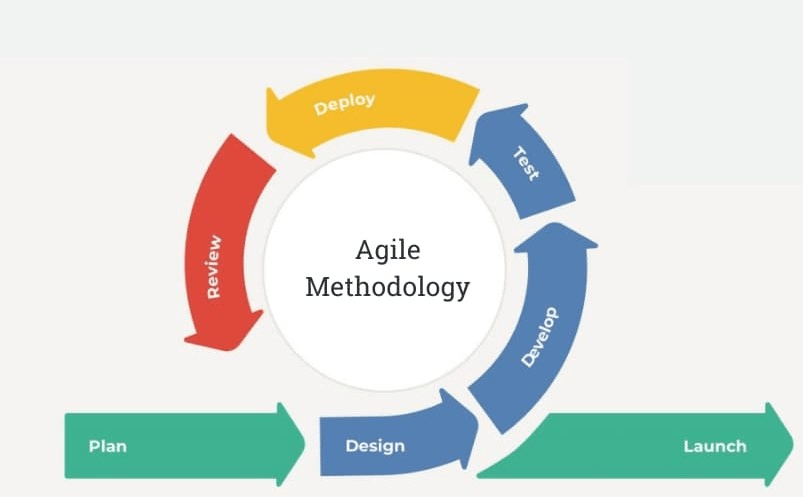
\includegraphics[width=0.85\linewidth,height=0.8\textheight,keepaspectratio]{Figures/agile_methodology.png}
\caption{Agile Methodology}
\label{fig:agilemethodology}
\end{figure}

\subsection{Justification of Proposing the Process Model}

The modules carry different levels of risk. Login, roles and exam set-up are well understood. Low-level Windows keyboard hooks, the live SignalR dashboard, webcam analysis and code execution in a Docker container were new to us. Waterfall would have forced us to fix all of these designs before we had built a prototype of any of them. With sprints we could try the risky parts early, integrate them step by step and adjust the plan. The sprint reviews at Weeks 16 and 32 also served as the FYP-I review and the final submission.

\subsection{Steps of Process Model}

The project runs over eight four-week sprints. Each sprint delivers modules that can be demonstrated. Table~\ref{tab:timeframe} in Chapter~\ref{chap:srs} gives the baseline schedule, and the text below it gives the progress at the FYP-I review. Every sprint goes through the following steps:
\begin{enumerate}[noitemsep]
\item \textbf{Product backlog:} FR1--FR12, grouped by module M1--M12 (Chapter~\ref{chap:srs}).
\item \textbf{Sprint planning:} a sprint goal and a sprint backlog in which each task has one WBS code and one owner.
\item \textbf{Development:} the module and its xUnit or Playwright tests are written in the same sprint.
\item \textbf{Increment:} a task is done when its code and tests pass and its thesis section is updated.
\item \textbf{Sprint review:} the increment is demonstrated to the supervisor, who comments on it and on the backlog priorities.
\item \textbf{Schedule check:} if under 80\% of the story points are done, backlog items are moved or cut (Chapter~\ref{chap:spp}).
\item \textbf{Feedback:} review comments and accepted changes return to the product backlog.
\end{enumerate}
The baseline plan gives each sprint the following work:

\begin{itemize}[noitemsep]
\item \textbf{Sprint 1 (Weeks 1--4):} requirements, use cases, product backlog, architecture and scope approval.
\item \textbf{Sprint 2 (Weeks 5--8):} M1 and M7, with HWID capture via Windows Management Instrumentation (WMI), device-bound student login, staff login and role-based access.
\item \textbf{Sprint 3 (Weeks 9--12):} M8 and M9, covering the exam wizard, question types, test cases, allowed applications and eligibility.
\item \textbf{Sprint 4 (Weeks 13--16):} M2, M3 and M4, covering the readiness check, practice exams, the student dashboard and the lockdown client.
\item \textbf{Sprint 5 (Weeks 17--20):} M5 and M10, with REST heartbeats, telemetry and screenshots, and the live SignalR dashboard.
\item \textbf{Sprint 6 (Weeks 21--24):} M6 and M11, covering autosave, encrypted backup, Docker test-case grading, TF-IDF theory scoring and the plagiarism matrix.
\item \textbf{Sprint 7 (Weeks 25--28):} M12, covering the hash-chained audit log, analytics, QuestPDF reports, and Excel and evidence-ZIP exports.
\item \textbf{Sprint 8 (Weeks 29--32):} integration and system testing of all twelve modules, bug fixes, the final report and the demonstration.
\end{itemize}

\chapter{SOFTWARE REQUIREMENTS SPECIFICATION}
\label{chap:srs}

This chapter gives the Software Requirements Specification (SRS) for SmartExam \cite{srs1}. It states what the system must do, the quality levels it must meet, and the limits it works within. How each feature is built is covered in the design chapters.

\section{Introduction}
SmartExam has five user roles, several exam phases and strict fairness rules. We wrote this SRS after interviews with lab staff, prototype walk-throughs and two team brainstorming sessions (Section~\ref{sec:gathering}).

\subsection{Document Scope}
The SRS covers the twelve modules M1--M12: authentication and device binding, pre-exam verification and practice exams, the student exam dashboard, the secure exam environment, the live monitoring client service, submission and backup, user and role management, exam creation and configuration, eligibility and access control, the live proctoring dashboard, AI-assisted evaluation, and logs, analytics and the audit trail. It also sets ten non-functional requirements (NFR1--NFR10) for security, reliability, usability, performance, maintainability, data integrity, compatibility, connectivity, privacy, and backup and recovery.

Database schemas, API routes, screen layouts and deployment settings are not part of this chapter. They are given in the design chapters.

\subsection{Audience}
\begin{itemize}
    \item \textbf{Project team:} the SRS is our contract. Every requirement maps to a module and to test cases. We do not build a feature that is not listed here unless the SRS is updated first.
    \item \textbf{Supervisor and evaluators:} they use it to judge whether the scope is clear and realistic for a two-semester FYP.
    \item \textbf{Future maintainers:} lab administrators, university IT staff or later FYP groups can use it to see what the system does and where it can be extended.
\end{itemize}

\section{Functional Requirements}
Table~\ref{tab:functionalrequirements} lists the functional requirements. FR$n$ belongs to module M$n$; module M11 has three (FR11.1--FR11.3). Each requirement states the limits that the tests in Chapter~\ref{chap:testing} check. Two rules apply across these requirements. Roles are kept apart, so only staff with access to an exam can read its monitoring data \cite{rbac1}. No penalty is automatic: the \texttt{ViolationClassifier} labels events, and all AI marks are suggestions that the teacher accepts or overrides; every override is audited.

{\small
\renewcommand{\arraystretch}{1.2}
\begin{longtable}{>{\raggedright\arraybackslash}p{1.3cm}>{\raggedright\arraybackslash}p{2.8cm}>{\raggedright\arraybackslash}p{10.3cm}}
\caption{Functional Requirements Mapped to Modules}
\label{tab:functionalrequirements}\\
\hline\hline
\textbf{ID} & \textbf{Module} & \textbf{Description} \\
\hline\hline
\endfirsthead
\multicolumn{3}{c}{\tablename~\thetable{} -- continued from previous page}\\
\hline\hline
\textbf{ID} & \textbf{Module} & \textbf{Description} \\
\hline\hline
\endhead
\hline \multicolumn{3}{r}{Continued on next page}\\
\endfoot
\hline\hline
\endlastfoot
FR1 & M1 Authentication and Device Binding & Log users in, allowing at most 10 login requests per minute from one IP address. Bind each student account to one workstation: the client sends its hardware ID (HWID: BIOS, system-disk and baseboard serials), the server stores only its SHA-256 hash, and a login from another PC is refused until an administrator resets the binding. Store passwords as salted PBKDF2 (Password-Based Key Derivation Function 2) hashes \cite{rfc8018} and issue JWTs \cite{rfc7519} that expire after 30 min, with single-use rotating refresh tokens. \\
FR2 & M2 Pre-Exam Verification and Practice Exam & Before an exam, check the network (best API round trip at most 2 s), clock skew (at most 60 s from the server), screen capture, webcam, microphone, secure mode (one monitor, no Remote Desktop Protocol (RDP) session, no virtual machine (VM), keyboard hook active) and free disk (at least 200 MB). When an exam requires readiness, a pass older than 30 min must be repeated. Offer practice exams with unlimited attempts, in Report lockdown mode and without the webcam; practice exams do not count towards results (they are auto-marked but never plagiarism-checked and are hidden from the student's results). \\
FR3 & M3 Student Exam Dashboard & In the desktop client, show the student's current assigned exam with its instructions, start countdown, readiness status and eligibility; Start stays disabled, with the reason shown, while the student is ineligible. List the practice exams. In the student web portal, show the student's exams, results (once the exam has ended), violation history, performance trend and notifications. Exams can be taken only in the desktop client. \\
FR4 & M4 Secure Exam Environment & Run a fullscreen, topmost exam window; block Alt+Tab, the Windows key and Task Manager; guard the clipboard; report unauthorised processes (Report mode) or also close them (Enforce mode); detect newly mounted USB storage devices, extra monitors, remote sessions and VMs. \\
FR5 & M5 Live Monitoring Client Service & Send a REST heartbeat every 10 s (focus, processes, idle time, camera status) and monitoring events in batches every 5 s. Take screenshots at random intervals around a per-exam mean (default 60 s, i.e. 30--90 s; 10--600 s allowed) and immediately on a violation. When the exam requires the webcam, analyse frames on the PC for seven issues (camera unavailable, covered or frozen; no face; multiple faces; head turned away, by a coarse head-pose check; phone in view), send one event per episode, and upload webcam snapshots at the exam's interval and when an issue is raised. \\
FR6 & M6 Submission and Backup & Save each edited answer to the server 10 s after its first unsaved edit, and at once on a question change, focus loss or submit. Write every edit within about 1 s to an AES-256-GCM encrypted local backup, queue failed saves while offline and replay them in order, and after a crash resume with the server and backup answers merged. Return a SHA-256 receipt of the stored answers on submission. Enforce the deadline on the server (exam end plus the student's extra minutes and a 2-minute grace) and finalise overdue sessions as Timed out. \\
FR7 & M7 User and Role Management & Let administrators create, edit, import (CSV), deactivate and delete accounts, force a logout, reset a device binding and assign the roles SuperAdmin, Admin, Teacher, Invigilator and Student; only a SuperAdmin may create or manage Admin and SuperAdmin accounts. Let administrators maintain the academic structure of departments and courses. \\
FR8 & M8 Exam Creation and Configuration & Let teachers and administrators create exams with multiple-choice (MCQ), coding and theory questions, test cases, an allowed-apps list, a lockdown mode (Off, Report or Enforce; default Report), the webcam requirement, and the screenshot and webcam intervals. Let them announce an exam and notify its students of the schedule and of their grades, in the app and by email (SMTP). \\
FR9 & M9 Eligibility and Access Control & Set eligibility from imported attendance (default minimum 75\%) with audited manual overrides. Let administrators manage labs and workstations, and let the teacher assign invigilators and a workstation to each student. Allow the exam only from the assigned workstation (matched by machine name by default). \\
FR10 & M10 Live Proctoring Dashboard & Show a live tile per student over SignalR: Stable (Normal), Warning, Suspicious or Critical (Violation) from the event classes, Disconnected after 30 s of silence, and Submitted, Force submitted or Timed out at the end. Let staff (invigilators only on their assigned exams) send warnings, extend one student's time (1--180 min per grant, at most 600 min in total), unlock the PC (5 min from the drawer; the server allows 1--30 min) and relock it, record incidents (Low to Critical), force a submission, and view each student's timeline, screenshots and webcam snapshots. Commands reach the client in its next heartbeat reply. \\
FR11.1 & M11 AI-Assisted Evaluation & Compile C and C++ coding answers and run them against weighted test cases (default limit 2 s per case) in an isolated Docker \texttt{gcc:13} container when Docker is available; otherwise use a local MinGW g++ runner, which is not isolated, and with no runner leave the answer for teacher review. \\
FR11.2 & M11 AI-Assisted Evaluation & Mark MCQ answers as full or zero. Score theory answers against the model answer with offline TF-IDF similarity \cite{salton1988} (0.7 cosine similarity plus 0.3 key-term coverage) and a confidence value. Large language model (LLM) grading is optional and off by default. \\
FR11.3 & M11 AI-Assisted Evaluation & Compare the submissions of each non-practice exam pairwise by k-gram winnowing \cite{winnowing} (k = 5, window 4), show a similarity matrix, and flag pairs at or above the exam's threshold (default 70\%) for the teacher. \\
FR12 & M12 Logs, Analytics and Audit Trail & Keep a tamper-evident audit log of security-relevant and staff actions, in which each row is chained to the previous one by a SHA-256 hash, and let administrators verify the chain. Produce exam analytics, an exam summary PDF, separate attendance, violations and scores PDFs, an Excel workbook and an evidence ZIP with a SHA-256 manifest; each export is audited with its file hash. \\
\end{longtable}}

\section{Non-Functional Requirements}
Non-functional requirements set quality levels and operating limits. We give them the identifiers NFR1--NFR10 and split them into quality attributes, based on ISO/IEC 25010:2023 \cite{iso25010}, and other requirements.

\subsection{Quality Attributes}
Table~\ref{tab:nonfunctionalrequirements} gives NFR1--NFR6. Where our name differs from the standard, the ISO/IEC 25010 characteristic is shown in brackets.

{\small
\renewcommand{\arraystretch}{1.2}
\begin{longtable}{>{\raggedright\arraybackslash}p{1.3cm}>{\raggedright\arraybackslash}p{2.9cm}>{\raggedright\arraybackslash}p{10.2cm}}
\caption{Quality Attributes}
\label{tab:nonfunctionalrequirements}\\
\hline\hline
\textbf{ID} & \textbf{Attribute} & \textbf{Requirement} \\
\hline\hline
\endfirsthead
\multicolumn{3}{c}{\tablename~\thetable{} -- continued from previous page}\\
\hline\hline
\textbf{ID} & \textbf{Attribute} & \textbf{Requirement} \\
\hline\hline
\endhead
\hline \multicolumn{3}{r}{Continued on next page}\\
\endfoot
\hline\hline
\endlastfoot
NFR1 & Security & Passwords are stored as PBKDF2-HMAC-SHA256 hashes with a 32-byte salt and 600,000 iterations \cite{owasp_pwd}; the iteration count is stored with each hash, so older hashes are upgraded at the next login \cite{nist80063b}. Access tokens expire after 30 min; refresh tokens are single-use and rotate, and reusing one revokes its whole family. Login allows 10 and refresh 30 requests per minute per IP address, then returns HTTP 429. Every endpoint except the two login endpoints, token refresh and the health check requires a valid JWT and a permitted role. In a lab deployment all traffic shall use HTTPS (NFR8). \\
NFR2 & Reliability & A network outage of any length shall not lose an answer: every edit reaches the encrypted local backup within about 1 s, failed saves and monitoring events are queued and sent in order when the server is reachable again, and a restarted client resumes the session. An automatic submit at time-out retries every 10 s until the server answers. \\
NFR3 & Usability (interaction capability) & A student shall be able to log in, pass the readiness check and start an exam using only the on-screen instructions. Every refusal (failed check, ineligibility, wrong workstation, failed login) shows its reason, and final actions (submitting with unanswered questions, force-submitting) ask for confirmation. \\
NFR4 & Performance (performance efficiency) & With 40 desktop clients (the upper end of the 30--40 lab machines in Section~\ref{sec:productpurpose}) sending heartbeats every 10 s, login, exam start, answer saves and heartbeats shall complete within 2 s at the 95th percentile. The readiness check fails a PC whose best API round trip exceeds 2 s. \\
NFR5 & Maintainability & One ASP.NET Core 9 API organised by module. Every module M1--M12 has automated tests (xUnit for the API and client logic, Playwright for the web panel) that run headless, so a full regression needs no lab PC. \\
NFR6 & Data Integrity (security: integrity) & The server enforces the deadline, so a changed client clock cannot extend an exam. A save with an older revision than the stored answer is refused. Each submission returns a SHA-256 receipt of the stored answers, and verifying the hash-chained audit log reveals a changed row or a gap in the sequence. \\
\end{longtable}}

\subsection{Other Non-Functional Requirements}
Table~\ref{tab:othernfr} gives NFR7--NFR10, the platform, connectivity, privacy and recovery constraints.

{\small
\renewcommand{\arraystretch}{1.2}
\begin{longtable}{>{\raggedright\arraybackslash}p{1.3cm}>{\raggedright\arraybackslash}p{2.9cm}>{\raggedright\arraybackslash}p{10.2cm}}
\caption{Other Non-Functional Requirements}
\label{tab:othernfr}\\
\hline\hline
\textbf{ID} & \textbf{Category} & \textbf{Requirement} \\
\hline\hline
\endfirsthead
\multicolumn{3}{c}{\tablename~\thetable{} -- continued from previous page}\\
\hline\hline
\textbf{ID} & \textbf{Category} & \textbf{Requirement} \\
\hline\hline
\endhead
\hline \multicolumn{3}{r}{Continued on next page}\\
\endfoot
\hline\hline
\endlastfoot
NFR7 & Compatibility & Client on Windows 10 (22H2) or Windows 11 with the .NET 9 Desktop Runtime; tested on Windows 11. Web panel in Chrome or Edge 111 or later (the build target); tested on the Chromium bundled with Playwright. \\
NFR8 & Connectivity & The client and the web panel call the API over REST, using plain HTTP on the shipped localhost configuration and HTTPS behind a TLS endpoint in a lab deployment; the API itself does not enforce HTTPS. No local lab server is needed. SignalR carries live updates between the API and the web dashboard; the desktop client uses REST only and receives invigilator warnings, extra time, unlocks and force-submits in the reply to its next heartbeat (every 10 s). \\
NFR9 & Privacy & No face recognition or identity matching is performed. When an exam requires the webcam, frames are analysed on the PC (camera unavailable, covered or frozen, no face, multiple faces, head turned away, phone in view); webcam snapshots are uploaded at the exam's interval and when an issue is raised, can be viewed only by the exam's owner, its assigned invigilators and administrators, and are deleted after 30 days. The same access rule and 30-day retention apply to screenshots. \\
NFR10 & Backup and Recovery & The database (Neon PostgreSQL) shall be restorable to a point in time within the provider's restore window. A crash on a student PC loses at most the last second of typing, because answers are restored from the encrypted local backup. Screenshots and webcam snapshots are kept on the API server's disk, which the database backup does not cover, so the evidence folder shall be copied to backed-up storage after each exam; generated reports are not backed up because they can be produced again from the database. \\
\end{longtable}}

\section{Requirement Gathering Techniques Used}
\label{sec:gathering}

We used structured interviews, paper prototypes and two brainstorming sessions \cite{elicit1, sommerville}.

\subsection{Interviews}
We asked teachers and lab coordinators how practical exams run today. Two needs came up most: watching workstations live, and keeping evidence that can settle disputes later.

\subsection{Prototyping}
We showed users paper prototypes of the login, dashboard, exam and submission screens \cite{sommerville}. Their feedback added a countdown timer on the exam screen, live alerts at the top of the teacher dashboard, and one question per screen.

\subsection{Brainstorming Session 1: Academic Workflow}
We mapped the life cycle of a lab exam and the manual steps that cost staff the most time. This set the order in which we built the foundation: role management, exam configuration and seat assignment (Sprints 2 and 3).

\subsection{Brainstorming Session 2: Monitoring and Reporting}
We discussed monitoring, proctoring and reports. Face recognition was left out of scope because of privacy concerns and the effort of reliable identity matching on lab webcams, so the webcam checks look only at the camera state and the faces in view; the coarse head-pose and phone checks were added later. We also agreed that every exam needs reports on attendance, violations and scores; these became separate PDF exports beside an exam summary PDF.

\section{Time Frame}
The project runs over eight four-week sprints (Weeks 1--32), each ending with a working increment for supervisor review (Table~\ref{tab:timeframe}).

\begin{table}[H]
\centering
\caption{Project Time Frame (8 Sprints)}
\label{tab:timeframe}
\renewcommand{\arraystretch}{1.25}
\begin{tabular}{l>{\raggedright\arraybackslash}p{8.2cm}c}
\hline\hline
\textbf{Sprint} & \textbf{Major Activities} & \textbf{Duration} \\
\hline\hline
Sprint 1 (Weeks 1--4)   & Requirement analysis, product backlog, architecture and scope approval. & 4 Weeks \\
Sprint 2 (Weeks 5--8)   & M1, M7: login, hardware-ID device binding, JWT and roles. & 4 Weeks \\
Sprint 3 (Weeks 9--12)  & M8, M9: exam creation, test cases, allowed apps, eligibility and seats. & 4 Weeks \\
Sprint 4 (Weeks 13--16) & M2, M3, M4: readiness check, practice exams, student dashboard, lockdown. & 4 Weeks \\
Sprint 5 (Weeks 17--20) & M5, M10: monitoring client and live proctoring dashboard. & 4 Weeks \\
Sprint 6 (Weeks 21--24) & M6, M11: autosave and backup, test-case grading, theory scoring, plagiarism. & 4 Weeks \\
Sprint 7 (Weeks 25--28) & M12: hash-chained audit log, analytics, QuestPDF reports, and Excel and evidence-ZIP exports. & 4 Weeks \\
Sprint 8 (Weeks 29--32) & Integration, end-to-end testing, bug fixing, documentation and demo. & 4 Weeks \\
\hline\hline
\end{tabular}
\end{table}

Table~\ref{tab:timeframe} is the baseline plan. It fits the FYP-I proposal's timeline (February 2026 to March 2027) into two semesters: Week 1 began in March 2026 and Week 32 ended with the final test run on 26 October 2026, and installation in the labs follows submission. At the FYP-I review (Week 16), M1, M3, M7, M8, M9 and M10 (at heartbeat level) were working; M2, M4 and refresh-token rotation moved into Sprints 5--8 with the remaining modules.

\chapter{SOFTWARE PROJECT PLAN}
\label{chap:spp}

This chapter explains how we plan, schedule and control the project over two semesters \cite{pmbok6}. The twelve modules depend on each other: exam creation feeds eligibility, the monitoring client feeds the live dashboard, and both feed the final reports. A delay in an early module therefore delays the later ones. The chapter covers the deliverables, the project management plan (planning, Gantt chart, work breakdown and critical path), the managerial process, and risk management.

\textbf{Project Overview.} SmartExam runs a programming lab exam from start to finish: device-bound sign-in and lockdown on the lab workstations, live supervision, AI-assisted marking and an audit trail. It serves the students, teachers, invigilators and administrators of a department (Chapter~\ref{chap:introduction}).

\textbf{Project Organization.} Three members share the work: the project manager also owns the backend and the database, and each of the other two members owns one area, the desktop client or AI evaluation and testing (Section~\ref{sec:managerial}). We use a light form of Scrum, and our supervisor reviews the result of every sprint.

\textbf{Project Schedule.} The work runs in eight four-week sprints over Weeks 1--32 (Table~\ref{tab:timeframe}); the milestones are in Section~\ref{sec:milestones} and the Gantt chart and critical path in Section~\ref{sec:scheduling}.

\textbf{Resource Allocation.} The people, hardware, software and services that the project uses, and their cost, are given in the Resources Plan (Section~\ref{sec:resources_plan}).

\section{Deliverables of the Project}

A deliverable is a concrete output that we hand over and that can be checked \cite{del1}. Our deliverables fall into five groups.

\subsection{Requirements and Analysis Deliverables}
These are the problem statement, the scope statement, the review of existing systems, the record of our interviews and brainstorming sessions (Section~\ref{sec:gathering}), and the Software Requirements Specification: the functional and non-functional requirements in Chapter~\ref{chap:srs}. Together they fix the goals and boundaries of the system \cite{srs1}.

\subsection{Design Deliverables}
These are the system architecture, the module breakdown, the use case diagram, the ERD, the data flow diagrams, the UML structure and behaviour diagrams, and the user interface designs and physical database design of Chapter~\ref{chap:system_interface_physical_design}. They split the system into modules that we can assign to team members and sprints.

\subsection{Prototype and Module Deliverables}
A working system of twelve modules, built as three parts:
\begin{enumerate}
    \item \textbf{Student WPF client:} device-bound login, readiness check, lockdown, live monitoring, autosave and encrypted local backup.
    \item \textbf{React web panel:} user and exam management, eligibility, the live proctoring dashboard over SignalR, grade review and reports.
    \item \textbf{ASP.NET Core 9 API:} authentication, exam and eligibility rules, monitoring intake, the violation classifier, AI-assisted evaluation and audit logging, with data in Neon PostgreSQL.
\end{enumerate}
A module counts as delivered when its API endpoints pass the xUnit integration tests, its web screens pass the Playwright end-to-end tests and its desktop logic passes the client unit tests. Checks that need a real lab PC are tracked as pending lab verification (Table~\ref{tab:st_pending}).

\subsection{Testing and Validation Deliverables}
These are unit and API integration tests (xUnit with an in-memory database), headless browser tests (Playwright with a simulated student client), manual lab checklists, and the test plan and test report (Chapter~\ref{chap:testing}), which list the results and known limits.

\subsection{Documentation and Presentation Deliverables}
These are this report, the presentation slides and our responses to supervisor feedback.

\section{Software Project Management Plan}

\subsection{Project Planning}

We plan in eight four-week sprints (Table~\ref{tab:timeframe}). Sprint 1 covers requirements and architecture, Sprints 2--7 deliver the modules, and Sprint 8 is for integration, testing and the demonstration. A task is done when its code and tests pass and its thesis section is updated.

\subsubsection{Work Breakdown Structure}

The Work Breakdown Structure (WBS) splits the project into work packages \cite{wbs1}. Figure~\ref{fig:wbs} goes down to module level: each module is one work package (2.x.y) that includes its own tests, so package 3 (Sprint 8) holds only system-level work: final integration, end-to-end tests, the full regression run and bug fixing. In the sprint backlog each module is split further into tasks, and each task has one WBS code and one owner from the role split in Section~\ref{sec:managerial}.

\begin{figure}[!htbp]
\centering
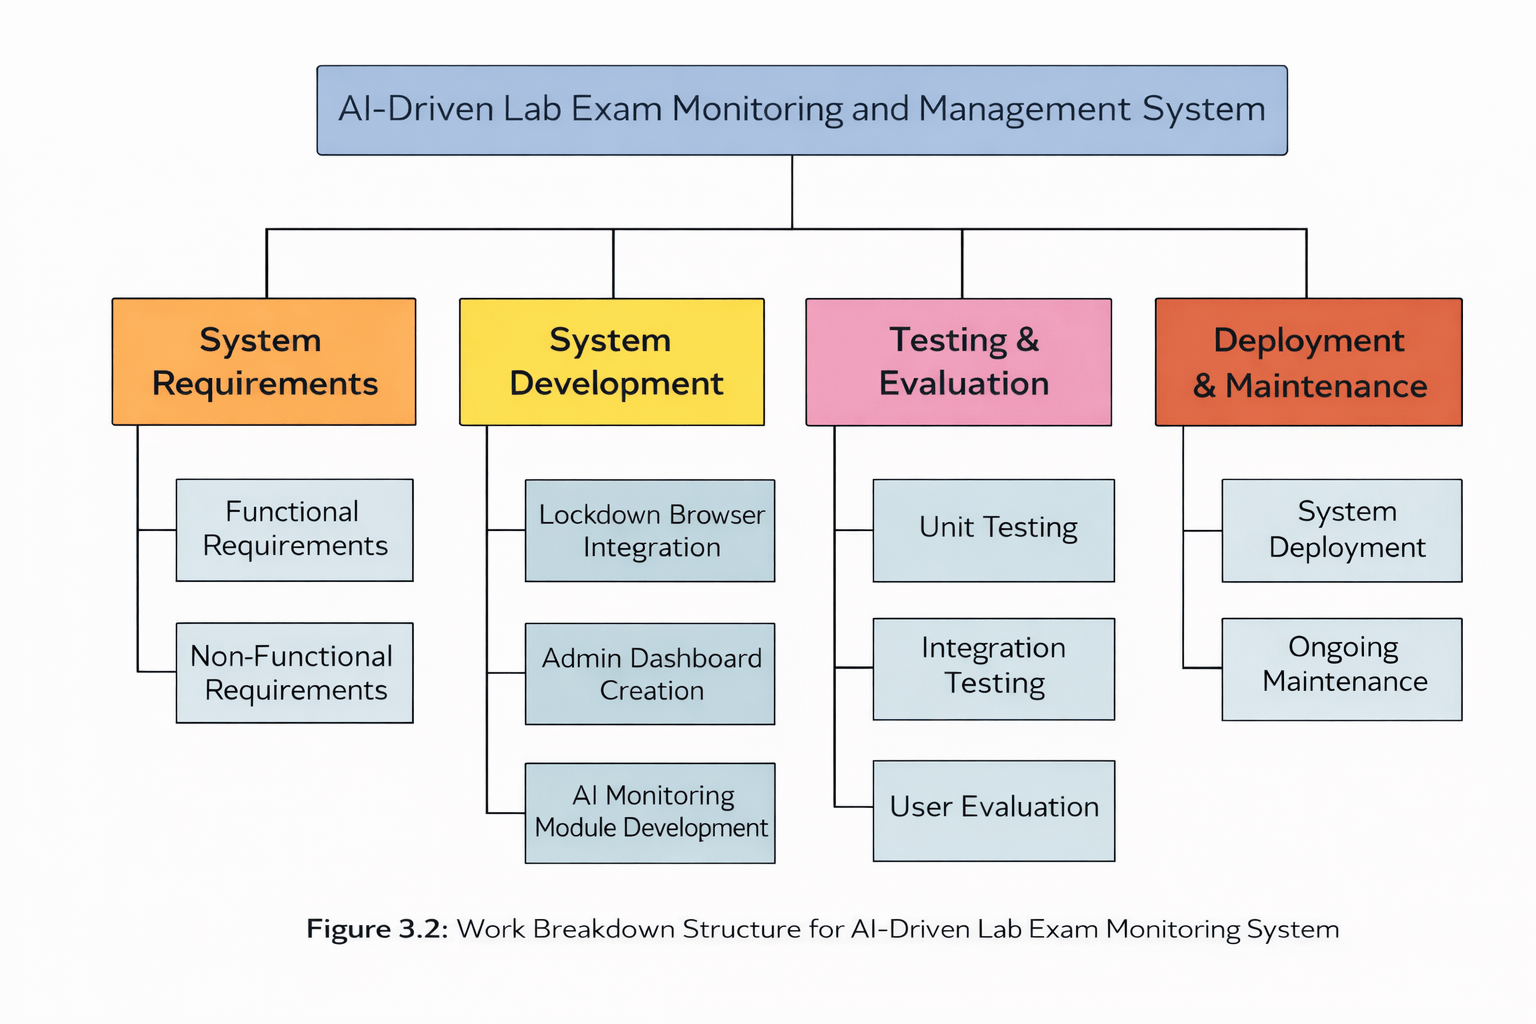
\includegraphics[width=\linewidth]{Figures/work_breakdown_structure.png}
\caption{Work Breakdown Structure}
\label{fig:wbs}
\end{figure}

\subsection{Project Scheduling}

\subsubsection{Gantt Chart}

Figure~\ref{fig:ganttchart} shows the baseline plan of Table~\ref{tab:timeframe}: one bar for each activity of Table~\ref{tab:cpm}, with arrows for its dependencies \cite{gantt1}. The progress actually reached at the FYP-I review is given below Table~\ref{tab:timeframe}.

\begin{figure}[!tb]
\centering
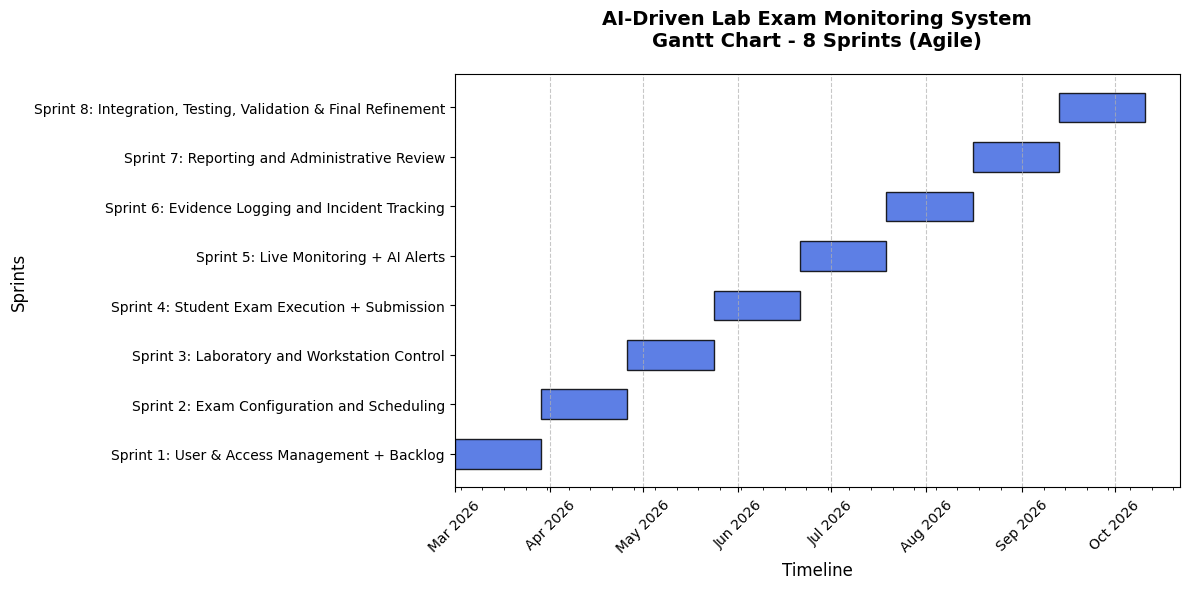
\includegraphics[width=\linewidth]{Figures/gantt_chart.png}
\caption{Project Gantt Chart (Baseline Plan, Eight Sprints)}
\label{fig:ganttchart}
\end{figure}

\subsubsection{Critical Path Method}

The critical path is the longest chain of dependent activities; any delay on it delays the project \cite[Sec.~6.5.2.2]{pmbok6}. Table~\ref{tab:cpm} lists our activities and Figure~\ref{fig:criticalpath} shows the network.

\begin{table}[!htbp]
\centering
\caption{Project Activities, Durations and Dependencies}
\label{tab:cpm}
\renewcommand{\arraystretch}{1.2}
\begin{tabular}{c>{\raggedright\arraybackslash}p{7.2cm}lcc}
\hline\hline
\textbf{ID} & \textbf{Activity} & \textbf{Modules} & \textbf{Weeks} & \textbf{Depends on} \\
\hline\hline
A & Requirements, backlog and architecture & -- & 4 & -- \\
B & Authentication and device binding & M1 & 4 & A \\
C & User and role management & M7 & 2 & A \\
D & Exam creation and eligibility & M8, M9 & 4 & B, C \\
E & Readiness check, student dashboard and lockdown & M2--M4 & 4 & D \\
F & Monitoring client and live proctoring dashboard & M5, M10 & 4 & E \\
G & Submission, backup and AI-assisted evaluation & M6, M11 & 4 & F \\
H & Hash-chained audit log, analytics and reports & M12 & 4 & G \\
I & Integration, system testing, documentation and demo & All & 4 & H \\
\hline\hline
\end{tabular}
\end{table}

The critical path is A $\rightarrow$ B $\rightarrow$ D $\rightarrow$ E $\rightarrow$ F $\rightarrow$ G $\rightarrow$ H $\rightarrow$ I, which takes 32 weeks ($8 \times 4$); the only other chain, through C, takes 30 weeks. Only C has float: it takes two weeks alongside B, so it can slip two weeks without moving the end date. Since almost all work is on the critical path, a late sprint delays every later one.

\begin{figure}[!htbp]
\centering
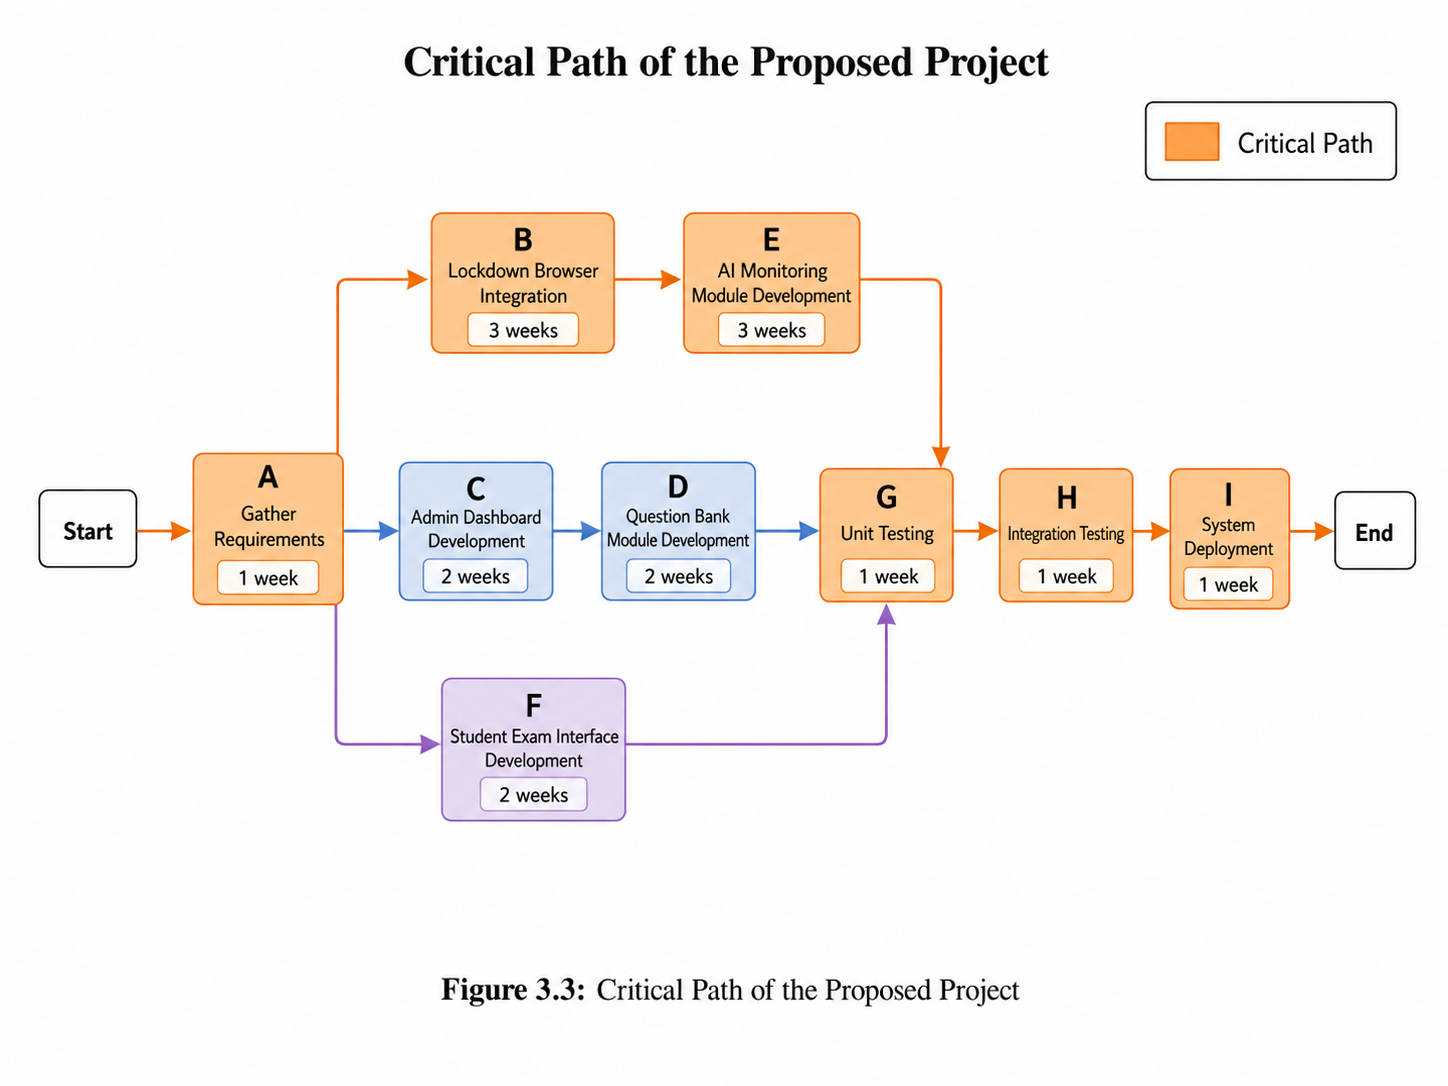
\includegraphics[width=0.95\linewidth]{Figures/critical_path.png}
\caption{Critical Path Network}
\label{fig:criticalpath}
\end{figure}

\subsubsection{Schedule Control}

We track progress with sprint burn-down charts \cite{scrum1}. If less than 80\% of a sprint's story points are done at the review, we hold a recovery meeting and move or cut backlog items before the next sprint starts.

\section{Managerial Process}
\label{sec:managerial}

Our three-member team follows a few simple rules for priorities, communication and change \cite{pmbok6}. The roles are those of the FYP-I proposal: Muhammad Haider Ali is project manager and owns the architecture, backend API and database; Zain Ali Mehmood owns the student desktop application, lockdown and monitoring client; and Roshaan Ali Shah owns AI evaluation, plagiarism detection, and testing and validation.

\subsection{Management Objectives and Priorities}

Our objective is a system that lets a teacher run a fair lab exam from start to finish.

\DiagramBarrier
\textbf{Goals.} We measure progress towards it with four goals:
\begin{itemize}
    \item Deliver all twelve modules, each with its own tests, within the 32 weeks, and end with a full regression run in Week 32.
    \item Test every functional requirement FR1--FR12 (Chapter~\ref{chap:testing}), and keep any check that needs a lab PC on the lab checklist.
    \item Use no paid services.
    \item Show the supervisor a working increment at the end of every sprint.
\end{itemize}

\textbf{Priorities.} When time is short, we protect work in this order:
\begin{enumerate}
    \item \textbf{Foundations:} roles and accounts, exam creation and the student dashboard (M7, M8, M3).
    \item \textbf{Exam integrity:} device binding, the readiness check, eligibility and seat checks, and lockdown (M1, M2, M9, M4).
    \item \textbf{No lost work:} autosave, encrypted backup and server deadline enforcement (M6).
    \item \textbf{Live supervision:} monitoring client and proctoring dashboard (M5, M10).
    \item \textbf{Evaluation support:} test-case grading, theory scoring and plagiarism checks (M11).
    \item \textbf{Reporting:} audit logs, analytics and PDF reports (M12).
\end{enumerate}
Lower items are cut first.

\subsection{Assumptions and Constraints}
\label{sec:constraints}

\textbf{Assumptions}
\begin{itemize}
    \item Lab PCs run Windows 10 or 11 (we tested on Windows 11), and we can install the client with administrator rights.
    \item Each PC reaches the API over the lab network, through HTTPS at a TLS endpoint in deployment (the shipped localhost configuration is plain HTTP); short outages may happen.
    \item Each student uses one assigned workstation, with a webcam when the exam needs one.
    \item Teachers supply test cases and model answers for automated grading.
\end{itemize}

\textbf{Constraints}
\begin{itemize}
    \item Three members and 32 weeks over two semesters.
    \item No budget for paid services: we use the Neon free tier, and AI features run offline on the CPU (TF-IDF scoring, OpenCV YuNet face detection \cite{yunet} and YOLOX-Nano phone detection \cite{yolox}). LLM grading is off by default.
    \item The client is Windows-only (WPF) and cannot block Ctrl+Alt+Del.
    \item Isolated code execution (C and C++ only) needs Docker on the grading server. Without it, a local MinGW runner that is not isolated is used, and with no runner the answer is left for the teacher.
    \item For privacy, no face recognition or identity matching is performed. Screenshots and webcam snapshots can be viewed only by the exam's owner, its assigned invigilators and administrators, and are deleted after 30 days.
\end{itemize}

\subsection{Communication, Review and Change Control}

We follow the Scrum framework in a light form \cite{scrumguide2020}. Each sprint opens with Sprint Planning, where we set the sprint goal from the product backlog, and ends with a Sprint Review of the results with our supervisor, whose feedback goes into the next sprint's backlog. Short written check-ins replace the daily stand-up \cite{scrum1}, and a blocker unsolved after 24 hours goes to a team discussion. A proposed change is accepted only if it improves the project, fits in the sprint and does not put a working module at risk \cite[Sec.~4.6]{pmbok6}. Otherwise it goes to the future-work list.

\textbf{Changes since the FYP-I proposal.} The twelve proposal modules were regrouped. Role management moved to M7 and device authorisation joined login in M1. Exam scheduling joined exam creation (M8), and the scheduling dashboard became M3. Behaviour analysis became the violation classifier used by M5 and M10, and eligibility, a Phase-1 item of the proposal, became its own module (M9). We added the Invigilator role to separate supervision from exam ownership, and the SuperAdmin role to guard the Admin accounts. Of the two databases the proposal allowed, we chose PostgreSQL, hosted on Neon. Grading and plagiarism checks run inside the C\# API instead of the optional Python microservice, which avoids a second runtime. The prototype uses this cloud database; moving it to a university-hosted server is a deployment step that is not yet done.

\section{Project Risk Management}

We identify risks early, rate them, and plan one response for each \cite{risk1}.

\subsection{Risk Management Plan}

\subsubsection{Purpose}

The plan sets how we find, rate, answer and track the risks that could stop a fair exam or delay the 32-week schedule, and who does each step.

\subsubsection{Roles and Responsibilities}

\begin{description}
    \item[Risk Manager and Project Manager:] Muhammad Haider Ali keeps the risk register (Table~\ref{tab:risk_matrix}) and owns the schedule, academic and staffing risks R8--R10 (owner PM).
    \item[Risk Analysts and Owners:] each area owner rates the risks of that area and carries out their responses: Zain Ali Mehmood for the desktop client (Client), Muhammad Haider Ali for the API and database (Backend), and Roshaan Ali Shah for AI evaluation and quality assurance (AI/QA).
    \item[Project Team Members:] all three members report a new risk at the written check-ins (Section~\ref{sec:managerial}).
    \item[Stakeholders:] our supervisor, Ms.~Zainab Iftikhar Chaudhary, sees the re-rated risks at each Sprint Review.
\end{description}

\subsection{Risk Management Activities}

\subsubsection{Risk Identification}

We identified twelve risks and placed each in one of four categories: technical, schedule, academic or resource (the Category column of Table~\ref{tab:risk_matrix}).

\subsubsection{Risk Analysis}

Table~\ref{tab:risk_matrix} rates each risk for likelihood and impact on a consequence/likelihood matrix \cite{iec31010}. With Low = 1, Medium = 2 and High = 3, the priority is likelihood $\times$ impact: 6--9 is High, 3--4 Medium and 1--2 Low. The Owner column names the area from the roles above.

\begin{table}[!tb]
\centering
\caption{Risk Likelihood and Impact Assessment}
\label{tab:risk_matrix}
{\footnotesize\setlength{\tabcolsep}{3pt}\renewcommand{\arraystretch}{1.2}
\begin{tabularx}{\textwidth}{@{}c>{\raggedright\arraybackslash}Xlcccll@{}}
\hline\hline
\textbf{ID} & \textbf{Risk} & \textbf{Category} & \textbf{Likelihood} & \textbf{Impact} & \textbf{Priority} & \textbf{Owner} & \textbf{Response} \\ \hline
R1 & Hardware ID spoofing or virtual machine use & Technical & Medium & High & High & Client & Mitigate \\
R2 & Lockdown bypass, or antivirus blocking the hooks & Technical & Medium & High & High & Client & Mitigate \\
R3 & Network loss during an exam & Technical & Medium & High & High & Client & Mitigate \\
R4 & API or database overload during live monitoring & Technical & Low & High & Medium & Backend & Mitigate \\
R5 & Inconsistent automated grading & Technical & Medium & Medium & Medium & AI/QA & Mitigate \\
R6 & Runtime or library end of support & Technical & Medium & Medium & Medium & Backend & Mitigate \\
R7 & Exposure of student data or records & Technical & Low & High & Medium & Backend & Mitigate \\
R8 & Incomplete module integration before the deadline & Schedule & Medium & High & High & PM & Mitigate \\
R9 & Thesis text drifting from the implementation & Academic & Medium & Medium & Medium & PM & Mitigate \\
R10 & Team member unavailable during a critical sprint & Resource & Low & Medium & Low & PM & Mitigate \\
R11 & Lab workstations unavailable for testing & Resource & Low & High & Medium & AI/QA & Mitigate \\
R12 & False webcam alerts (lighting, camera angle, slow CPU) & Technical & Medium & Medium & Medium & Client & Mitigate \\ \hline\hline
\end{tabularx}}
\end{table}

\subsubsection{Risk Response Planning}

A risk can be avoided, transferred to another party, mitigated or accepted. All twelve of our responses are mitigations that lower the likelihood, the impact or both; no risk is passed to another party or left without action. Each response below matches the risk with the same ID in Table~\ref{tab:risk_matrix}.

\begin{description}
    \item[R1:] The client reads the BIOS, system-disk and baseboard serials; the server hashes them with SHA-256 and binds the account to that hash at the first login. Logins from another device are refused (\texttt{DEVICE\_MISMATCH}). Virtual machines and Remote Desktop sessions fail the readiness Secure-mode check and are reported by \texttt{DeviceGuardService} during the exam.
    \item[R2:] A low-level keyboard hook blocks Alt+Tab and the Windows key, Task Manager is disabled, and the exam window stays fullscreen and topmost. Ctrl+Alt+Del cannot be blocked, so focus loss is logged. If antivirus blocks the keyboard hook, the readiness Secure-mode check fails in Report and Enforce mode alike; if the hook or the Task Manager policy fails during the exam, the client sends \texttt{LockdownDegraded}, which the invigilator sees on the tile. The lab then adds the client to the antivirus allow-list; failing that, the teacher turns off the readiness requirement for that exam and the invigilator watches that seat. Report mode helps only when antivirus stops the client from closing applications.
    \item[R3:] Every edit is written within about 1 s to an AES-256-GCM encrypted local backup, and each answer is saved to the server 10 s after its first unsaved edit (at once on a question change, focus loss or submit). Failed saves are queued and resent on reconnect, the client restores answers after a crash, and an automatic submit at the deadline retries every 10 s. The teacher can extend time.
    \item[R4:] The client sends a small REST heartbeat every 10 s, which the server stores only when it changes or every 60 s. Screenshots are taken at random intervals around the exam's mean (30--90 s by default) or on a violation, with at most 30 per minute per session. SignalR is used only between the API and the web dashboard; the desktop client receives warnings in its heartbeat reply. We check Neon usage weekly.
    \item[R5:] Coding answers run in a fixed \texttt{gcc:13} Docker image when Docker is available (otherwise in a local MinGW runner, which is not isolated, or they are left for the teacher). Theory scoring uses deterministic TF-IDF, and LLM grading is off by default. Teachers review and can override every mark.
    \item[R6:] The API and the client target .NET~9, a standard-term release whose support ends in November 2026, so we plan to move to .NET~10 (long-term support) once the full test suite passes on it. NuGet versions are fixed in the project files and npm versions in \texttt{package-lock.json}, and are updated only when the full test suite passes.
    \item[R7:] Passwords are stored as salted PBKDF2-HMAC-SHA256 hashes (600,000 iterations). Every endpoint except the two login endpoints, token refresh and the health check requires a valid JWT and a permitted role. In deployment, traffic uses HTTPS through a TLS endpoint; the API itself does not enforce HTTPS, and the shipped localhost configuration is plain HTTP. No face recognition is performed, and screenshots and webcam snapshots are visible only to the exam's owner, its invigilators and administrators and are deleted after 30 days.
    \item[R8:] Each module is merged with its xUnit tests, and its web screens with headless Playwright tests, so modules are integrated as they are built. Sprint 8 adds no new modules: it is kept for final integration, the full regression run and fixes.
    \item[R9:] Updating the thesis section is part of each task's definition of done.
    \item[R10:] Work is split by area (Section~\ref{sec:managerial}) in a shared Git repository, so another member can take over a module.
    \item[R11:] Most tests run on our own PCs against an in-memory backend. Lab PCs are booked only for manual lockdown and webcam checks before each demo.
    \item[R12:] Frames are analysed on the PC, and each finding must persist before it is raised: no face for 5 s, several faces or the head turned away for 3 s, and a phone in two consecutive checks. The head turn is measured against the student's own baseline. An issue sends one event with a webcam snapshot; the classifier only labels it, no penalty is automatic, and the invigilator decides. The readiness check tests the camera before the exam.
\end{description}

\subsubsection{Risk Monitoring and Control}

The owners re-rate their risks at every Sprint Review. A risk that rises to High is taken to the supervisor at that review with a recovery action, as for a sprint below the 80\% burn-down mark (Section~\ref{sec:schedule_control}). A new risk takes the next free ID, and a risk is closed when it can no longer occur; for example, R8 can be closed once the final regression run of Week 32 passes.

\chapter{FUNCTIONAL ANALYSIS AND MODELING}

\section{Use Case Modeling}

A use case model describes the system from the user's side \cite{uml_systems_analysis}. It fixed the scope early, so that the student client and the web panel were built against the same set of actions.

The subject is the whole SmartExam system: the WPF desktop client and the React web panel, with the API behind them. The human actors are the five roles of the \texttt{UserRole} enum. A \textbf{Student} sits exams in the desktop client and uses the web portal for results, violations, performance and notifications. An \textbf{Invigilator} supervises only the exams they are assigned to through the \texttt{ExamProctors} table, and cannot edit exams or grade. A \textbf{Teacher} also configures exams, eligibility, seating and announcements and reviews marks and the similarity matrix. An \textbf{Admin} manages users, departments, courses, labs and device bindings and reads the audit log and system analytics, and only a \textbf{SuperAdmin} manages Admin and SuperAdmin accounts. The staff roles form a generalisation chain, so an Admin inherits every Teacher use case and can also create and edit exams. The email server is a secondary, external actor. Figures~\ref{fig:usecase_diagram} and~\ref{fig:usecase_diagram_b} show the 27 use cases, each with its ID and requirement: the student's use cases with live supervision, then the staff use cases (UC-12, sign-in, appears in both); an \texttt{<<include>>} arrow points to the use case that is always part of the base, and an \texttt{<<extend>>} arrow points from an optional behaviour to the base it extends.

\begin{figure}[!htbp]
\centering
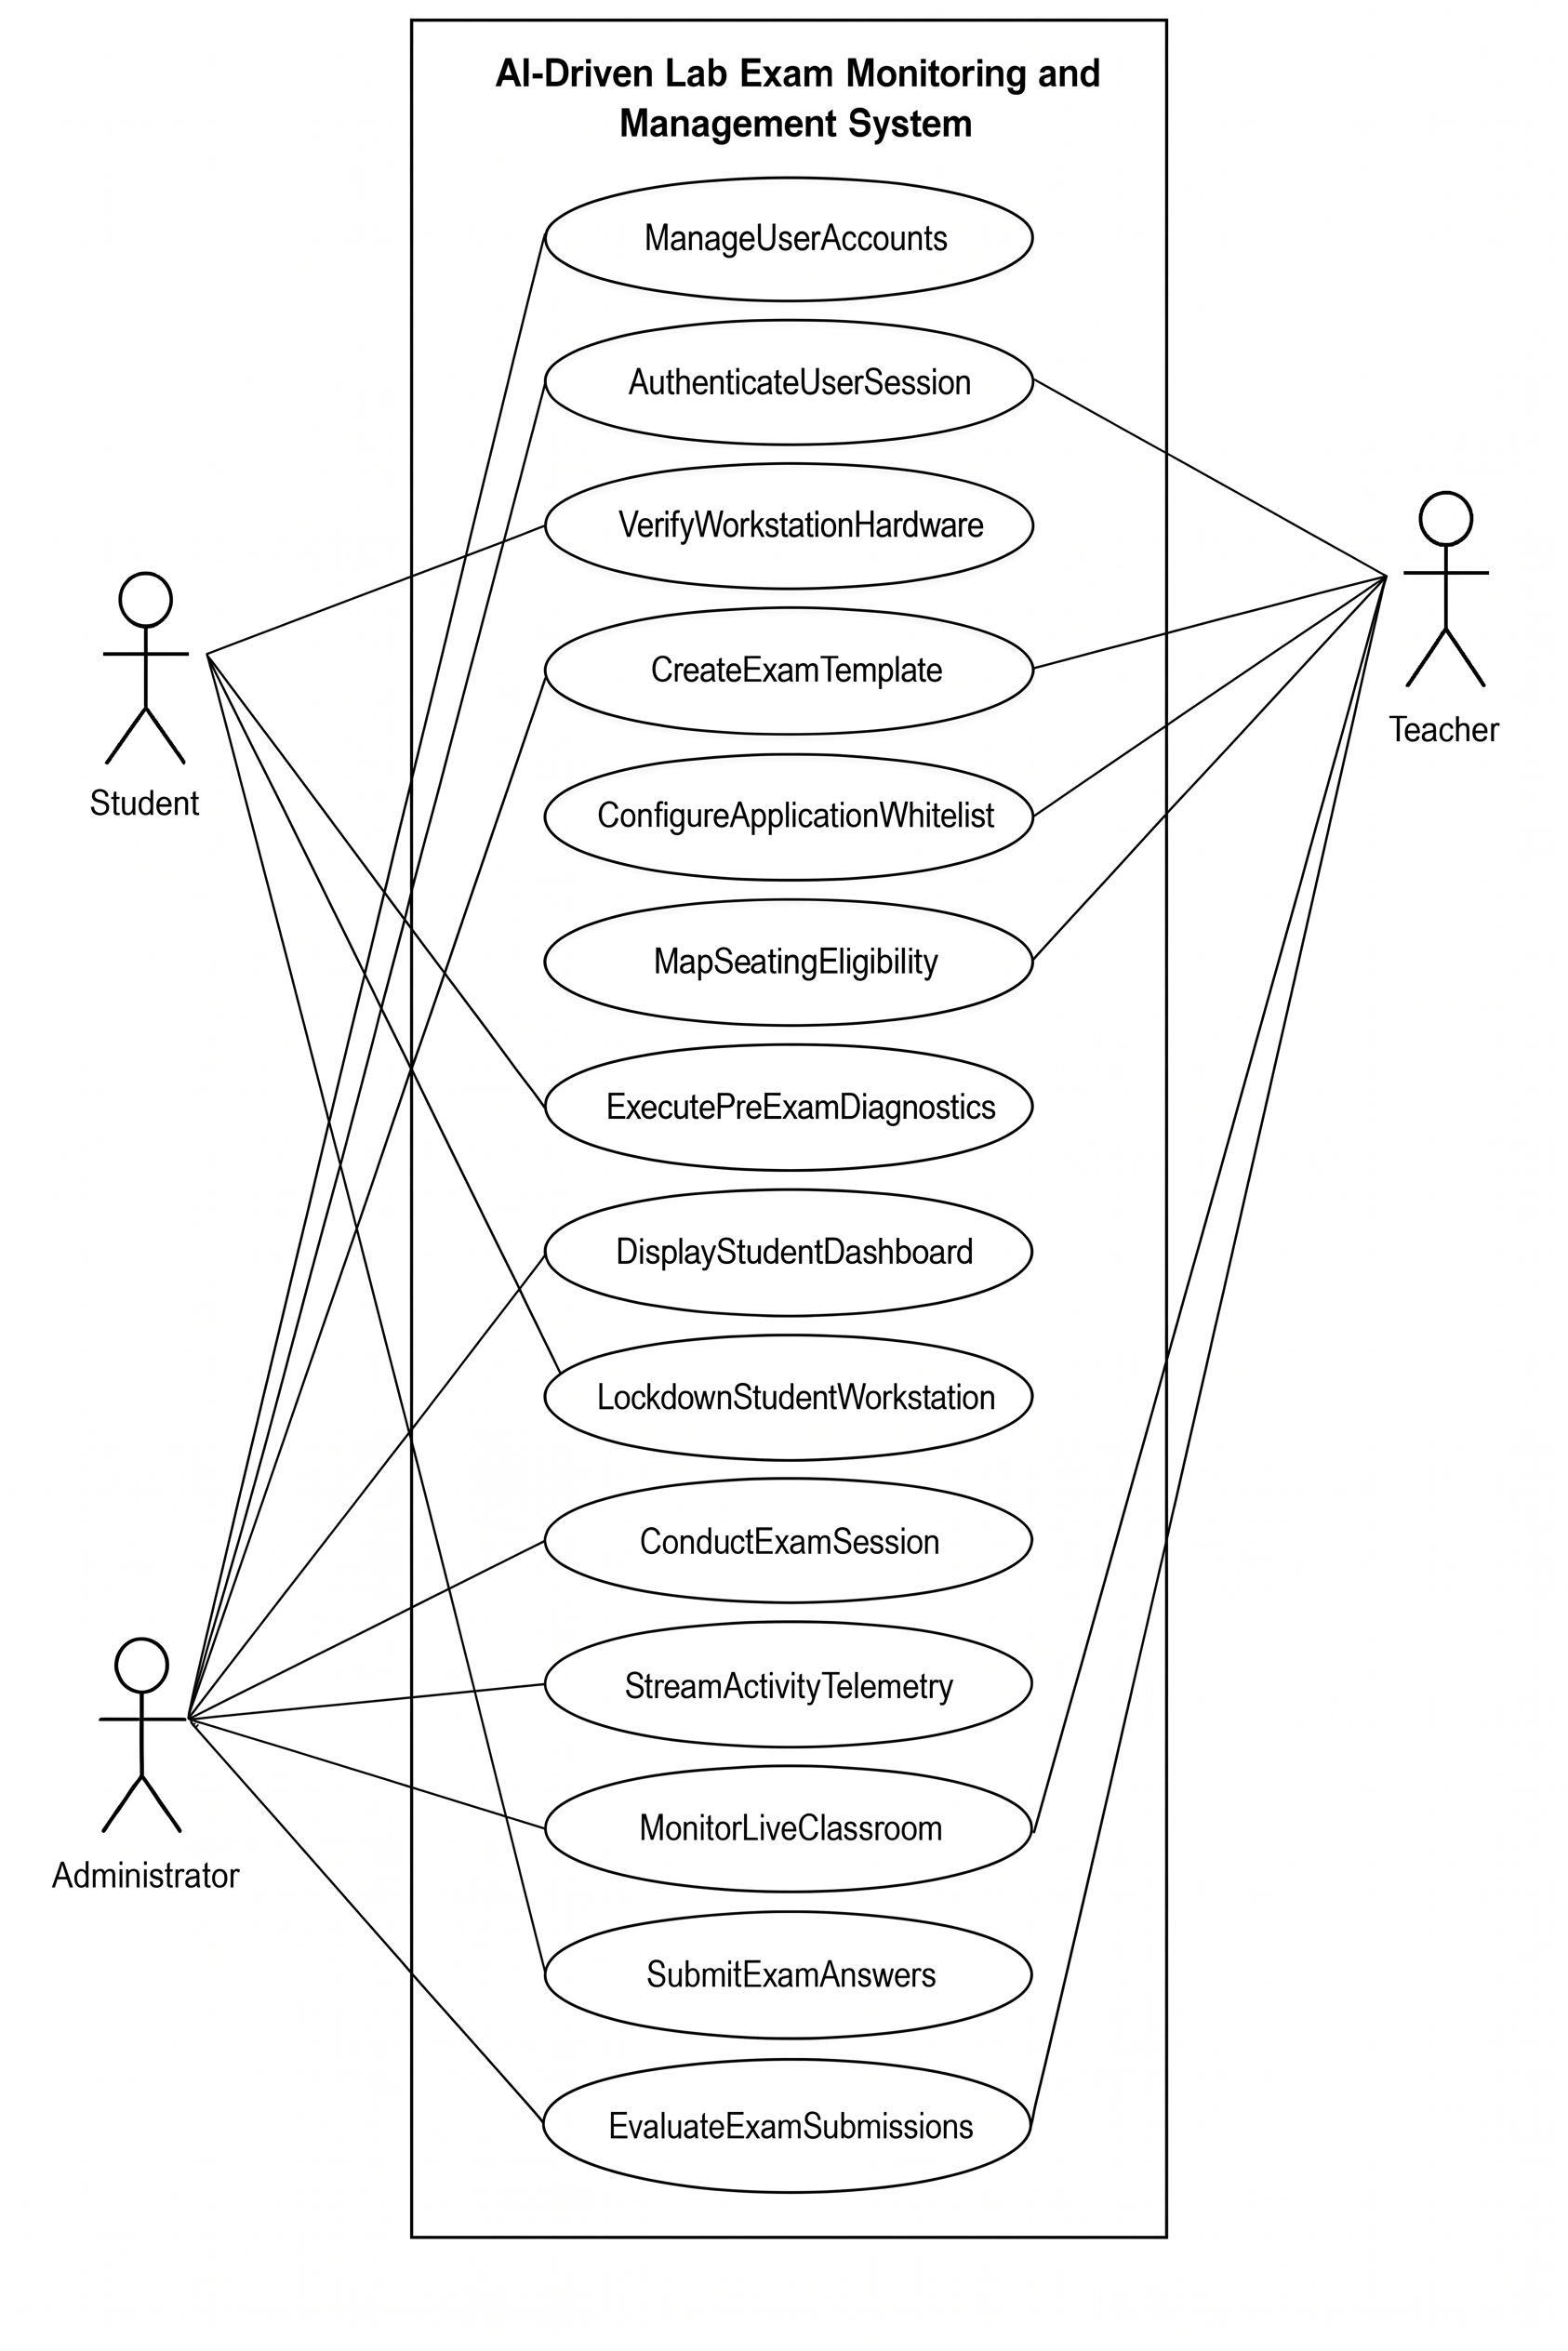
\includegraphics[width=\linewidth,height=0.9\textheight,keepaspectratio]{Figures/use_case_diagram.png}
\caption{Use Case Diagram of SmartExam (a): Student and Invigilator Use Cases}
\label{fig:usecase_diagram}
\end{figure}

\begin{figure}[!htbp]
\centering
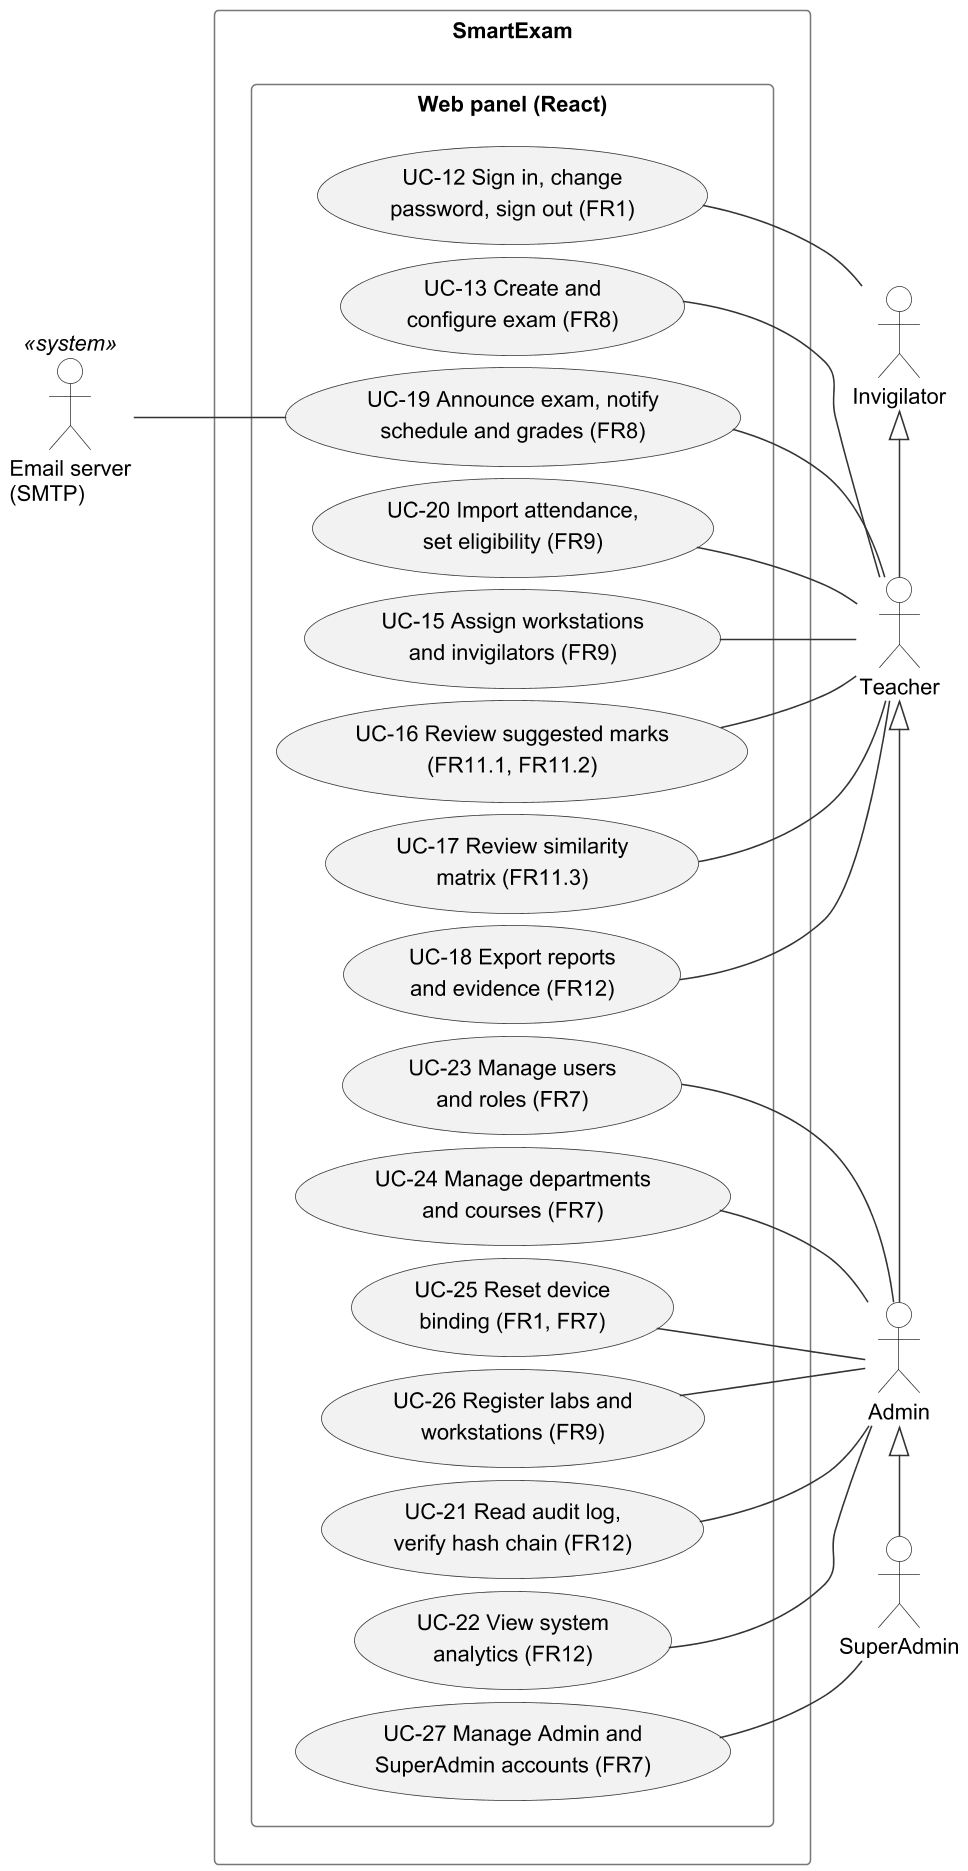
\includegraphics[width=\linewidth,height=0.9\textheight,keepaspectratio]{Figures/use_case_diagram_b.png}
\caption{Use Case Diagram of SmartExam (b): Staff Use Cases of the Web Panel}
\label{fig:usecase_diagram_b}
\end{figure}

\begin{sloppypar}
The API enforces this separation. Role attributes (\texttt{[Authorize(Roles=...)]}) restrict the endpoints, and \texttt{ExamAccessService} checks who may supervise a given exam.
\end{sloppypar}

\subsection{User Stories}

We wrote user stories to plan sprints and to define when a feature was done \cite{user_stories_applied}. Each story names the requirement it serves.

\subsubsection{Student}
\begin{enumerate}[nosep]
    \item As a student, I log in from the client and my account is bound to my lab PC, so nobody can sit my exam from another machine (FR1).
    \item As a student, I run a system check and a practice exam that does not count towards my results, so problems with my PC show up early (FR2).
    \item As a student, I see my assigned exam with the start countdown, my check status and whether I am eligible; Start stays disabled, with the reason, if I am not (FR3).
    \item As a student, I sit the exam in a locked fullscreen window where unapproved apps are reported, or closed in Enforce mode, so every candidate works under the same rules (FR4).
    \item As a student, I have my answers saved every 10 seconds and kept on the PC while the network is down, and I get a receipt hash when I submit (FR6).
    \item As a student, I see an invigilator's warning or extra time on my screen during the exam (FR10).
    \item As a student, I see my results once the exam has ended, my violation history, performance and notifications on the web portal (FR3).
\end{enumerate}

\subsubsection{Teacher}
\begin{enumerate}[nosep,resume]
    \item As a teacher, I create an exam with MCQ, coding and theory questions, test cases, an allowed-apps list and a lockdown mode, and announce it to the students (FR8).
    \item As a teacher, I import attendance, override eligibility (each override is audited), and assign each student a workstation (FR9).
    \item As a teacher, I get screenshots at random 30--90~s intervals (by default) and on each violation, plus idle time and webcam status, as evidence (FR5).
    \item As a teacher, I watch live student tiles, open a student's timeline and screenshots, and warn, extend time, unlock the PC or force-submit (FR10).
    \item As a teacher, I get coding answers run against weighted test cases and suggested marks for theory answers, which I can accept or override (FR11.1, FR11.2).
    \item As a teacher, I see a similarity matrix of submissions so that I can review likely copying myself (FR11.3).
    \item As a teacher, I export an exam's summary PDF, attendance, violations and scores reports, an Excel workbook and an evidence ZIP (FR12).
\end{enumerate}

\subsubsection{Invigilator}
\begin{enumerate}[nosep,resume]
    \item As an invigilator, I see only the exams I am assigned to and can warn students, extend time, unlock the PC, record incidents and force a submission, but not edit the exam or grade (FR10).
\end{enumerate}

\subsubsection{Admin and SuperAdmin}
\begin{enumerate}[nosep,resume]
    \item As an admin, I create, import, deactivate and sign out users, assign their roles, and maintain departments and courses (FR7).
    \item As an admin, I reset a student's device binding when a lab PC is replaced (FR1).
    \item As an admin, I register labs and workstations with their PC names and IP addresses so that seats can be enforced (FR9).
    \item As an admin, I filter the audit log by event type and verify its hash chain, to check logins, device bindings and eligibility overrides (FR12).
\end{enumerate}

\subsection{Individual Actor Use Cases}

Table~\ref{tab:uc_trace} maps each use case to its requirement. Tables~\ref{tab:uct_auth_device} to~\ref{tab:uct_audit} describe the main use case of each requirement in template fields \cite{use_case_definition}; the other use cases are simple record maintenance or views. Actors are people or external systems only.

\begin{table}[H]
\centering
\caption{Use Cases Traced to Functional Requirements}
\label{tab:uc_trace}
{\footnotesize\renewcommand{\arraystretch}{0.9}
\begin{tabularx}{\textwidth}{>{\raggedright\arraybackslash}p{3.0cm}>{\raggedright\arraybackslash}X>{\raggedright\arraybackslash}p{3.4cm}}
\hline\hline
\textbf{Requirement} & \textbf{Use cases (Figures~\ref{fig:usecase_diagram} and~\ref{fig:usecase_diagram_b})} & \textbf{Description} \\
\hline
FR1 & UC-01, UC-12, UC-25 & Table~\ref{tab:uct_auth_device} \\
FR2 & UC-02, UC-03 & Table~\ref{tab:uct_pre_exam_check} \\
FR3 & UC-04, UC-14 & Table~\ref{tab:uct_start_exam} \\
FR4 & UC-06 & Table~\ref{tab:uct_lockdown_telemetry} \\
FR5 & UC-07 & Table~\ref{tab:uct_lockdown_telemetry} \\
FR6 & UC-08 & Table~\ref{tab:uct_submit} \\
FR7 & UC-23, UC-24, UC-25, UC-27 & Table~\ref{tab:uct_users} \\
FR8 & UC-13, UC-19 & Table~\ref{tab:uct_exam_config} \\
FR9 & UC-04 (start checks), UC-15, UC-20, UC-26 & Table~\ref{tab:uct_eligibility} \\
FR10 & UC-05, UC-09, UC-10, UC-11 & Table~\ref{tab:uct_live_proctoring} \\
FR11.1, FR11.2 & UC-16 & Table~\ref{tab:uct_compilation_evaluation} \\
FR11.3 & UC-17 & Table~\ref{tab:uct_plagiarism} \\
FR12 & UC-18, UC-21, UC-22 & Tables~\ref{tab:uct_audit_report}, \ref{tab:uct_audit} \\
\hline\hline
\end{tabularx}}
\end{table}


% Use case tables (lead-in sentence kept in the first head)
\newlength{\UCindent}\setlength{\UCindent}{\parindent}

{\renewcommand{\arraystretch}{0.9}\setlength{\tabcolsep}{4pt}
\begin{longtable}{@{}>{\footnotesize\raggedleft\arraybackslash}p{0.25cm}>{\footnotesize\bfseries\raggedright\arraybackslash}p{3.3cm}>{\footnotesize\raggedright\arraybackslash}p{\dimexpr\textwidth-3.3cm-0.25cm-16pt\relax}@{}}
\multicolumn{3}{@{}p{\textwidth}@{}}{\normalsize\hspace*{\UCindent}Table~\ref{tab:uct_auth_device} describes UC-01 of module M1. All exam-time use cases of the student need the session it opens on the bound workstation; UC-12 (web sign-in, password change and sign-out) and UC-25 (binding reset) complete FR1.\par\vspace*{6pt}}\\
\caption{Use Case Table of Log In and Bind Device (UC-01, FR1)}\label{tab:uct_auth_device}\\ \hline\hline
\endfirsthead
\multicolumn{3}{c}{\footnotesize\tablename~\thetable{} -- continued from previous page}\\ \hline\hline
\endhead
\hline \multicolumn{3}{r}{\footnotesize Continued on next page}\\
\endfoot
\hline\hline
\endlastfoot
1 & UCT ID & UC-01 (FR1) \\* \noalign{\hrule}
2 & Case Name & Log In and Bind Device \\* \noalign{\hrule}
3 & Use-Case Overview & A student signs in on the desktop client, and the account is bound to one workstation. \\* \noalign{\hrule}
4 & Actors & Student \\* \noalign{\hrule}
5 & Pre-Conditions & Active student account; client running on a lab PC. \\* \noalign{\hrule}
6 & Triggers & Student presses Log in in the client. \\* \noalign{\hrule}
7 & Steps & 1.~Student enters email or roll number and password.\newline
2.~Client reads the BIOS, system-disk and baseboard serials and sends them, with the PC name, to the server together with the credentials.\newline
3.~Server checks the password hash and hashes the hardware ID with SHA-256.\newline
4.~At the first login the server binds the account to this hash (\texttt{DEVICE\_BOUND}); at every later login the hash must match.\newline
5.~Server opens a session with a 30-minute access token and a refresh token (\texttt{LOGIN\_SUCCESS}). \\ \hline
8 & Post-Conditions & Student is signed in on the bound workstation. \\ \hline
9 & Exception Flow & Wrong password or inactive account: 401, audited \texttt{LOGIN\_FAILED}. More than 10 login requests per minute from one IP: 429. Another PC: 401 \texttt{DEVICE\_MISMATCH}, audited; an admin must reset the binding (UC-25). \\
\end{longtable}}

{\renewcommand{\arraystretch}{0.9}\setlength{\tabcolsep}{4pt}
\begin{longtable}{@{}>{\footnotesize\raggedleft\arraybackslash}p{0.25cm}>{\footnotesize\bfseries\raggedright\arraybackslash}p{3.3cm}>{\footnotesize\raggedright\arraybackslash}p{\dimexpr\textwidth-3.3cm-0.25cm-16pt\relax}@{}}
\multicolumn{3}{@{}p{\textwidth}@{}}{\normalsize\hspace*{\UCindent}Table~\ref{tab:uct_pre_exam_check} describes UC-02 of module M2, which decides whether a PC is fit to start an exam. The other FR2 use case, the practice exam (UC-03), runs in the locked window of Table~\ref{tab:uct_lockdown_telemetry}.\par\vspace*{6pt}}\\
\caption{Use Case Table of Run Readiness Check (UC-02, FR2)}\label{tab:uct_pre_exam_check}\\ \hline\hline
\endfirsthead
\multicolumn{3}{c}{\footnotesize\tablename~\thetable{} -- continued from previous page}\\ \hline\hline
\endhead
\hline \multicolumn{3}{r}{\footnotesize Continued on next page}\\
\endfoot
\hline\hline
\endlastfoot
1 & UCT ID & UC-02 (FR2) \\* \noalign{\hrule}
2 & Case Name & Run Readiness Check \\* \noalign{\hrule}
3 & Use-Case Overview & The client checks that the PC can run the exam before Start is allowed. \\* \noalign{\hrule}
4 & Actors & Student \\* \noalign{\hrule}
5 & Pre-Conditions & Student is signed in (UC-01) and has an assigned exam. \\* \noalign{\hrule}
6 & Triggers & Student presses the system-check button on the dashboard. \\* \noalign{\hrule}
7 & Steps & 1.~Client checks the network (best API round trip at most 2~s), clock skew (at most 60~s), screen capture, webcam and microphone if the exam needs them, secure mode (one monitor, no RDP session or VM, keyboard hook active) and free disk (at least 200~MB).\newline
2.~Client shows each result.\newline
3.~Client sends the result to the server, which recomputes the pass, stores it and audits \texttt{READINESS\_PASSED} or \texttt{READINESS\_FAILED}. \\ \hline
8 & Post-Conditions & The result is stored and shown on the live monitor. \\ \hline
9 & Exception Flow & A failed check shows its reason; the student fixes it and retries. When the exam requires readiness, a pass older than 30~minutes must be repeated. \\
\end{longtable}}

{\renewcommand{\arraystretch}{0.9}\setlength{\tabcolsep}{4pt}
\begin{longtable}{@{}>{\footnotesize\raggedleft\arraybackslash}p{0.25cm}>{\footnotesize\bfseries\raggedright\arraybackslash}p{3.3cm}>{\footnotesize\raggedright\arraybackslash}p{\dimexpr\textwidth-3.3cm-0.25cm-16pt\relax}@{}}
\multicolumn{3}{@{}p{\textwidth}@{}}{\normalsize\hspace*{\UCindent}Table~\ref{tab:uct_start_exam} joins the student dashboard of module M3 with the start checks of module M9, so it shows every rule a student must meet before the exam opens. UC-14 covers the results side of FR3 on the web portal.\par\vspace*{6pt}}\\
\caption{Use Case Table of View Assigned Exam, Check In and Start (UC-04, FR3, FR9)}\label{tab:uct_start_exam}\\ \hline\hline
\endfirsthead
\multicolumn{3}{c}{\footnotesize\tablename~\thetable{} -- continued from previous page}\\ \hline\hline
\endhead
\hline \multicolumn{3}{r}{\footnotesize Continued on next page}\\
\endfoot
\hline\hline
\endlastfoot
1 & UCT ID & UC-04 (FR3, FR9) \\* \noalign{\hrule}
2 & Case Name & View Assigned Exam, Check In and Start \\* \noalign{\hrule}
3 & Use-Case Overview & The dashboard shows the student's assigned exam; the student checks in and starts it. \\* \noalign{\hrule}
4 & Actors & Student \\* \noalign{\hrule}
5 & Pre-Conditions & Student is signed in (UC-01). \\* \noalign{\hrule}
6 & Triggers & Student opens the dashboard after logging in. \\* \noalign{\hrule}
7 & Steps & 1.~Dashboard loads the assigned exam, its instructions, the server time and the eligibility, readiness and seat status.\newline
2.~Student presses Check In; the client records the attendance with the server.\newline
3.~Start becomes available at the opening time on the server clock, after check-in and, when the exam requires it, a readiness pass (UC-02).\newline
4.~Student presses Start; the server checks eligibility, the seat, the exam window and readiness, and opens an exam session. \\ \hline
8 & Post-Conditions & Session is \texttt{InProgress} and the exam window opens (UC-06). \\ \hline
9 & Exception Flow & Ineligible student: the exam is shown with the reason and Start stays disabled. Server refusals: \texttt{NOT\_ELIGIBLE}, \texttt{READINESS\_REQUIRED}, \texttt{EXAM\_NOT\_STARTED}, \texttt{EXAM\_CLOSED}, or 403 \texttt{SEAT\_MISMATCH} (audited and shown on the live monitor). Failed check-in: the student retries. \\
\end{longtable}}

{\renewcommand{\arraystretch}{0.9}\setlength{\tabcolsep}{4pt}
\begin{longtable}{@{}>{\footnotesize\raggedleft\arraybackslash}p{0.25cm}>{\footnotesize\bfseries\raggedright\arraybackslash}p{3.3cm}>{\footnotesize\raggedright\arraybackslash}p{\dimexpr\textwidth-3.3cm-0.25cm-16pt\relax}@{}}
\multicolumn{3}{@{}p{\textwidth}@{}}{\normalsize\hspace*{\UCindent}Table~\ref{tab:uct_lockdown_telemetry} combines UC-06 (module M4) and UC-07 (module M5), because the client locks the PC and reports on it from the same exam window. UC-05 extends it with the commands of the invigilator.\par\vspace*{6pt}}\\
\caption{Use Case Table of Sit the Locked Exam and Report to the API (UC-06 and UC-07, FR4, FR5)}\label{tab:uct_lockdown_telemetry}\\ \hline\hline
\endfirsthead
\multicolumn{3}{c}{\footnotesize\tablename~\thetable{} -- continued from previous page}\\ \hline\hline
\endhead
\hline \multicolumn{3}{r}{\footnotesize Continued on next page}\\
\endfoot
\hline\hline
\endlastfoot
1 & UCT ID & UC-06 and UC-07 (FR4, FR5) \\* \noalign{\hrule}
2 & Case Name & Sit the Locked Exam and Report to the API \\* \noalign{\hrule}
3 & Use-Case Overview & The student answers in a locked fullscreen window while the client guards the PC (UC-06) and reports its state and evidence (UC-07, included). Extended by UC-05. \\* \noalign{\hrule}
4 & Actors & Student \\* \noalign{\hrule}
5 & Pre-Conditions & Session is \texttt{InProgress}. \\* \noalign{\hrule}
6 & Triggers & A session starts (UC-04) or an interrupted session is resumed. \\* \noalign{\hrule}
7 & Steps & 1.~Exam window opens fullscreen and topmost; a low-level keyboard hook blocks Alt+Tab, the Windows key and Ctrl+Shift+Esc, and Task Manager is disabled.\newline
2.~Guards check processes every 2~s against the allowed apps (Report mode reports an unauthorised app, Enforce mode also closes it) and watch the clipboard, newly mounted USB storage, extra monitors, remote sessions and VMs.\newline
3.~Every 10~s the client sends a heartbeat with focus, processes, idle time and camera status, and the server passes it on to the live monitor.\newline
4.~Events are queued and sent in batches every 5~s; the server classifies each one and shows violations on the live monitor at once.\newline
5.~Screenshots are taken at random intervals around the exam's mean (30--90~s by default) and at once on a violation (at most one per 15~s), and uploaded through an encrypted local queue.\newline
6.~When the exam requires the webcam, frames are analysed on the PC for seven issues; one event is sent per episode, and webcam snapshots are uploaded at the exam's interval and when an issue is raised.\newline
7.~Student answers the questions and submits (UC-08). \\ \hline
8 & Post-Conditions & Events, screenshots and webcam snapshots are stored for the live monitor and the reports; the session ends through UC-08 and the PC is released. \\ \hline
9 & Exception Flow & A warning, extra time or unlock arrives in a heartbeat reply (UC-05); during an unlock monitoring continues and the client re-locks itself at the end. Network loss: events and captures stay in the queue and are sent later. No heartbeat for 30~s: the server marks the student Disconnected. A practice exam (UC-03) uses the same window in Report mode, without the webcam. \\
\end{longtable}}

{\renewcommand{\arraystretch}{0.9}\setlength{\tabcolsep}{4pt}
\begin{longtable}{@{}>{\footnotesize\raggedleft\arraybackslash}p{0.25cm}>{\footnotesize\bfseries\raggedright\arraybackslash}p{3.3cm}>{\footnotesize\raggedright\arraybackslash}p{\dimexpr\textwidth-3.3cm-0.25cm-16pt\relax}@{}}
\multicolumn{3}{@{}p{\textwidth}@{}}{\normalsize\hspace*{\UCindent}Table~\ref{tab:uct_submit} describes UC-08 of module M6. It is the use case in which a student's work could be lost, so its exception flow lists every recovery path.\par\vspace*{6pt}}\\
\caption{Use Case Table of Autosave and Submit Answers (UC-08, FR6)}\label{tab:uct_submit}\\ \hline\hline
\endfirsthead
\multicolumn{3}{c}{\footnotesize\tablename~\thetable{} -- continued from previous page}\\ \hline\hline
\endhead
\hline \multicolumn{3}{r}{\footnotesize Continued on next page}\\
\endfoot
\hline\hline
\endlastfoot
1 & UCT ID & UC-08 (FR6) \\* \noalign{\hrule}
2 & Case Name & Autosave and Submit Answers \\* \noalign{\hrule}
3 & Use-Case Overview & Answers are kept safe during the exam and submitted with a receipt. \\* \noalign{\hrule}
4 & Actors & Student \\* \noalign{\hrule}
5 & Pre-Conditions & Session is \texttt{InProgress}. \\* \noalign{\hrule}
6 & Triggers & Student edits an answer or presses Submit, or the timer expires. \\* \noalign{\hrule}
7 & Steps & 1.~Each edit is written within about 1~s to an AES-256-GCM encrypted local backup.\newline
2.~The answer is saved to the server 10~s after its first unsaved edit, and at once on a question change or focus loss.\newline
3.~Student presses Submit and confirms the number of unanswered questions.\newline
4.~Server finalises the session, returns a SHA-256 receipt of the stored answers, which the client checks, and queues the answers for grading. \\ \hline
8 & Post-Conditions & Session is \texttt{Submitted} or \texttt{TimedOut} with a stored receipt. \\ \hline
9 & Exception Flow & Network loss: failed saves are queued and replayed in order. Crash: answers are restored from the server and the backup. Timer expiry: the client submits automatically and retries every 10~s; the server times the session out 2~minutes after its end. Server unreachable on a manual submit: the window stays open and the student presses Submit again. \\
\end{longtable}}

{\renewcommand{\arraystretch}{0.9}\setlength{\tabcolsep}{4pt}
\begin{longtable}{@{}>{\footnotesize\raggedleft\arraybackslash}p{0.25cm}>{\footnotesize\bfseries\raggedright\arraybackslash}p{3.3cm}>{\footnotesize\raggedright\arraybackslash}p{\dimexpr\textwidth-3.3cm-0.25cm-16pt\relax}@{}}
\multicolumn{3}{@{}p{\textwidth}@{}}{\normalsize\hspace*{\UCindent}Table~\ref{tab:uct_users} describes UC-23 of module M7. UC-24 (departments and courses), UC-25 (binding reset) and UC-27 (Admin and SuperAdmin accounts) follow the same pattern of an audited change made by an administrator.\par\vspace*{6pt}}\\
\caption{Use Case Table of Manage Users and Roles (UC-23, FR7)}\label{tab:uct_users}\\ \hline\hline
\endfirsthead
\multicolumn{3}{c}{\footnotesize\tablename~\thetable{} -- continued from previous page}\\ \hline\hline
\endhead
\hline \multicolumn{3}{r}{\footnotesize Continued on next page}\\
\endfoot
\hline\hline
\endlastfoot
1 & UCT ID & UC-23 (FR7) \\* \noalign{\hrule}
2 & Case Name & Manage Users and Roles \\* \noalign{\hrule}
3 & Use-Case Overview & An administrator keeps the accounts and their roles. \\* \noalign{\hrule}
4 & Actors & Admin (a SuperAdmin for Admin and SuperAdmin accounts, UC-27) \\* \noalign{\hrule}
5 & Pre-Conditions & Admin is signed in. \\* \noalign{\hrule}
6 & Triggers & Admin opens the Users page. \\* \noalign{\hrule}
7 & Steps & 1.~Admin creates or edits a user and sets the role.\newline
2.~Admin imports users from a CSV file; each bad row is skipped with its line and reason (\texttt{USERS\_IMPORTED}).\newline
3.~Admin deactivates, activates or deletes a user, or forces a logout (\texttt{FORCE\_LOGOUT}); the user's next request is refused even if the access token has not expired.\newline
4.~Every change is audited (\texttt{USER\_*}). \\ \hline
8 & Post-Conditions & The account is stored; its role decides what the user may do. \\ \hline
9 & Exception Flow & Email already in use: 409. Unknown role: 400. An Admin creating or managing an Admin or SuperAdmin account: 403 \texttt{SUPERADMIN\_REQUIRED}, audited as \texttt{PRIVILEGED\_ACCOUNT\_DENIED}. \\
\end{longtable}}

{\renewcommand{\arraystretch}{0.9}\setlength{\tabcolsep}{4pt}
\begin{longtable}{@{}>{\footnotesize\raggedleft\arraybackslash}p{0.25cm}>{\footnotesize\bfseries\raggedright\arraybackslash}p{3.3cm}>{\footnotesize\raggedright\arraybackslash}p{\dimexpr\textwidth-3.3cm-0.25cm-16pt\relax}@{}}
\multicolumn{3}{@{}p{\textwidth}@{}}{\normalsize\hspace*{\UCindent}Table~\ref{tab:uct_exam_config} describes UC-13 of module M8, which sets the rules that the exam-time use cases enforce. UC-19 then announces the exam to its students.\par\vspace*{6pt}}\\
\caption{Use Case Table of Create and Configure an Exam (UC-13, FR8)}\label{tab:uct_exam_config}\\ \hline\hline
\endfirsthead
\multicolumn{3}{c}{\footnotesize\tablename~\thetable{} -- continued from previous page}\\ \hline\hline
\endhead
\hline \multicolumn{3}{r}{\footnotesize Continued on next page}\\
\endfoot
\hline\hline
\endlastfoot
1 & UCT ID & UC-13 (FR8) \\* \noalign{\hrule}
2 & Case Name & Create and Configure an Exam \\* \noalign{\hrule}
3 & Use-Case Overview & The teacher defines an exam, its questions and its lockdown rules. \\* \noalign{\hrule}
4 & Actors & Teacher (or an administrator) \\* \noalign{\hrule}
5 & Pre-Conditions & Teacher is signed in; the course section exists. \\* \noalign{\hrule}
6 & Triggers & Teacher opens the create-exam wizard. \\* \noalign{\hrule}
7 & Steps & 1.~Teacher enters title, start time, duration and instructions and selects the students to assign.\newline
2.~Teacher adds MCQ, coding and theory questions with marks, test cases (public or hidden) and reference answers.\newline
3.~Teacher sets allowed apps, lockdown mode (Off, Report or Enforce; default Report), readiness, webcam and microphone options, the screenshot and webcam intervals, early join, minimum attendance and seat enforcement.\newline
4.~Server validates and stores the exam (\texttt{EXAM\_CREATED}). \\ \hline
8 & Post-Conditions & Exam is \texttt{Scheduled}; students can be notified (UC-19). \\ \hline
9 & Exception Flow & Invalid fields, such as a capture interval outside 10--600~s, are rejected with 400. The teacher can edit the exam later (\texttt{EXAM\_UPDATED}) and add students to it. \\
\end{longtable}}

{\renewcommand{\arraystretch}{0.9}\setlength{\tabcolsep}{4pt}
\begin{longtable}{@{}>{\footnotesize\raggedleft\arraybackslash}p{0.25cm}>{\footnotesize\bfseries\raggedright\arraybackslash}p{3.3cm}>{\footnotesize\raggedright\arraybackslash}p{\dimexpr\textwidth-3.3cm-0.25cm-16pt\relax}@{}}
\multicolumn{3}{@{}p{\textwidth}@{}}{\normalsize\hspace*{\UCindent}Table~\ref{tab:uct_eligibility} describes UC-20 of module M9, which decides who may sit the exam. UC-15 (workstations and invigilators) and UC-26 (labs and workstations) supply the seat data that UC-04 checks.\par\vspace*{6pt}}\\
\caption{Use Case Table of Import Attendance and Set Eligibility (UC-20, FR9)}\label{tab:uct_eligibility}\\ \hline\hline
\endfirsthead
\multicolumn{3}{c}{\footnotesize\tablename~\thetable{} -- continued from previous page}\\ \hline\hline
\endhead
\hline \multicolumn{3}{r}{\footnotesize Continued on next page}\\
\endfoot
\hline\hline
\endlastfoot
1 & UCT ID & UC-20 (FR9) \\* \noalign{\hrule}
2 & Case Name & Import Attendance and Set Eligibility \\* \noalign{\hrule}
3 & Use-Case Overview & The teacher decides from attendance who may sit the exam. \\* \noalign{\hrule}
4 & Actors & Teacher (or an administrator) \\* \noalign{\hrule}
5 & Pre-Conditions & The exam exists and has assigned students (UC-13). \\* \noalign{\hrule}
6 & Triggers & Teacher opens the Eligibility page. \\* \noalign{\hrule}
7 & Steps & 1.~Teacher uploads the section's attendance CSV file (\texttt{ATTENDANCE\_IMPORTED}).\newline
2.~Teacher recalculates; students below the minimum (default 75\%) become ineligible (\texttt{ELIGIBILITY\_RECALCULATED}).\newline
3.~Teacher overrides individual students, with an optional note (\texttt{ELIGIBILITY\_OVERRIDDEN}).\newline
4.~Teacher assigns workstations and invigilators (UC-15). \\ \hline
8 & Post-Conditions & Every assignment has an eligibility; an ineligible student cannot start (UC-04). \\ \hline
9 & Exception Flow & Missing file, bad header or a file over 1~MB: 400; bad rows are reported per line. Recalculation after the exam has ended: 409. Overridden students are skipped by recalculation. \\
\end{longtable}}

{\renewcommand{\arraystretch}{0.9}\setlength{\tabcolsep}{4pt}
\begin{longtable}{@{}>{\footnotesize\raggedleft\arraybackslash}p{0.25cm}>{\footnotesize\bfseries\raggedright\arraybackslash}p{3.3cm}>{\footnotesize\raggedright\arraybackslash}p{\dimexpr\textwidth-3.3cm-0.25cm-16pt\relax}@{}}
\multicolumn{3}{@{}p{\textwidth}@{}}{\normalsize\hspace*{\UCindent}Table~\ref{tab:uct_live_proctoring} describes UC-10 of module M10, the invigilator's main screen, with UC-09 (evidence) and UC-11 (actions) as its optional extensions.\par\vspace*{6pt}}\\
\caption{Use Case Table of Supervise an Exam Live (UC-10, FR10)}\label{tab:uct_live_proctoring}\\ \hline\hline
\endfirsthead
\multicolumn{3}{c}{\footnotesize\tablename~\thetable{} -- continued from previous page}\\ \hline\hline
\endhead
\hline \multicolumn{3}{r}{\footnotesize Continued on next page}\\
\endfoot
\hline\hline
\endlastfoot
1 & UCT ID & UC-10 (FR10) \\* \noalign{\hrule}
2 & Case Name & Supervise an Exam Live \\* \noalign{\hrule}
3 & Use-Case Overview & Staff watch every student of a running exam and act on events. Extended by UC-09 and UC-11. \\* \noalign{\hrule}
4 & Actors & Invigilator (and, by inheritance, Teacher, Admin, SuperAdmin) \\* \noalign{\hrule}
5 & Pre-Conditions & Exam is running; the staff member owns it, is assigned to it or is an administrator. \\* \noalign{\hrule}
6 & Triggers & Staff member opens the Live Monitor and picks an exam. \\* \noalign{\hrule}
7 & Steps & 1.~The page subscribes to the live updates of the chosen exam.\newline
2.~Tiles update with each heartbeat and violation and show Stable (Normal), Warning, Suspicious or Critical (Violation); a finished session shows Submitted, Force submitted or Timed out.\newline
3.~Optionally (UC-09), the staff member opens a student's drawer to see the timeline, screenshots and webcam snapshots.\newline
4.~Optionally (UC-11), the staff member sends a warning, adds 1--180 minutes, unlocks the PC for five minutes from the drawer (the server allows 1--30 minutes) or relocks it, records an incident, or force-submits the session. \\ \hline
8 & Post-Conditions & Actions are audited; the client receives each command in its next heartbeat reply (UC-05). \\ \hline
9 & Exception Flow & No heartbeat for 30~s: the tile shows Disconnected until the client reconnects. Staff member without access to the exam: the server refuses the action. \\
\end{longtable}}

{\renewcommand{\arraystretch}{0.9}\setlength{\tabcolsep}{4pt}
\begin{longtable}{@{}>{\footnotesize\raggedleft\arraybackslash}p{0.25cm}>{\footnotesize\bfseries\raggedright\arraybackslash}p{3.3cm}>{\footnotesize\raggedright\arraybackslash}p{\dimexpr\textwidth-3.3cm-0.25cm-16pt\relax}@{}}
\multicolumn{3}{@{}p{\textwidth}@{}}{\normalsize\hspace*{\UCindent}Table~\ref{tab:uct_compilation_evaluation} covers FR11.1 and FR11.2 of module M11 in one use case, because the teacher reviews the code and theory marks on the same results screen.\par\vspace*{6pt}}\\
\caption{Use Case Table of Review Suggested Marks (UC-16, FR11.1, FR11.2)}\label{tab:uct_compilation_evaluation}\\ \hline\hline
\endfirsthead
\multicolumn{3}{c}{\footnotesize\tablename~\thetable{} -- continued from previous page}\\ \hline\hline
\endhead
\hline \multicolumn{3}{r}{\footnotesize Continued on next page}\\
\endfoot
\hline\hline
\endlastfoot
1 & UCT ID & UC-16 (FR11.1, FR11.2) \\* \noalign{\hrule}
2 & Case Name & Review Suggested Marks \\* \noalign{\hrule}
3 & Use-Case Overview & The grader suggests marks; the teacher accepts or changes them. \\* \noalign{\hrule}
4 & Actors & Teacher (or an administrator) \\* \noalign{\hrule}
5 & Pre-Conditions & Sessions are submitted, force-submitted or timed out, and the background grader has run. \\* \noalign{\hrule}
6 & Triggers & Teacher opens the results of an exam. \\* \noalign{\hrule}
7 & Steps & 1.~MCQ answers are marked full or zero.\newline
2.~C and C++ answers are compiled and run against each weighted test case (2~s per case by default) in an isolated Docker container (\texttt{gcc:13} image) when Docker is available, otherwise in a local MinGW g++ runner, which is not isolated.\newline
3.~Theory answers are scored against the reference answer by TF-IDF \cite{salton1988} (0.7 cosine similarity plus 0.3 key-term coverage) with a confidence value.\newline
4.~Teacher accepts all suggestions, overrides a mark with a note (\texttt{GRADE\_OVERRIDDEN}) or asks for an answer to be regraded. \\ \hline
8 & Post-Conditions & The suggested marks and the teacher's marks are stored separately. \\ \hline
9 & Exception Flow & Compile error or timeout: the test case fails and the message is shown. No runner available: the answer is left for a manual mark. Override outside 0 to the question's marks: 400. \\
\end{longtable}}

{\renewcommand{\arraystretch}{0.9}\setlength{\tabcolsep}{4pt}
\begin{longtable}{@{}>{\footnotesize\raggedleft\arraybackslash}p{0.25cm}>{\footnotesize\bfseries\raggedright\arraybackslash}p{3.3cm}>{\footnotesize\raggedright\arraybackslash}p{\dimexpr\textwidth-3.3cm-0.25cm-16pt\relax}@{}}
\multicolumn{3}{@{}p{\textwidth}@{}}{\normalsize\hspace*{\UCindent}Table~\ref{tab:uct_plagiarism} describes UC-17, the plagiarism part (FR11.3) of module M11, which works on the same submissions as UC-16.\par\vspace*{6pt}}\\
\caption{Use Case Table of Review the Similarity Matrix (UC-17, FR11.3)}\label{tab:uct_plagiarism}\\ \hline\hline
\endfirsthead
\multicolumn{3}{c}{\footnotesize\tablename~\thetable{} -- continued from previous page}\\ \hline\hline
\endhead
\hline \multicolumn{3}{r}{\footnotesize Continued on next page}\\
\endfoot
\hline\hline
\endlastfoot
1 & UCT ID & UC-17 (FR11.3) \\* \noalign{\hrule}
2 & Case Name & Review the Similarity Matrix \\* \noalign{\hrule}
3 & Use-Case Overview & The teacher sees how similar each pair of submissions is. \\* \noalign{\hrule}
4 & Actors & Teacher (or an administrator) \\* \noalign{\hrule}
5 & Pre-Conditions & A non-practice exam with finalised submissions. \\* \noalign{\hrule}
6 & Triggers & Teacher opens the plagiarism view of an exam. \\* \noalign{\hrule}
7 & Steps & 1.~At each submission, the answers are compared pairwise with the earlier ones by k-gram winnowing \cite{winnowing} (k = 5, window 4).\newline
2.~Teacher opens the similarity matrix for the whole exam or for one question.\newline
3.~Pairs at or above the exam's threshold (default 70\%) are flagged.\newline
4.~Teacher reviews the flagged pairs; no penalty is automatic. \\ \hline
8 & Post-Conditions & Flagged pairs stay listed; any change of marks goes through UC-16. \\ \hline
9 & Exception Flow & Practice exam: 400 \texttt{MOCK\_EXAM}. An MCQ question chosen: 400 \texttt{INVALID\_QUESTION}. \\
\end{longtable}}

{\renewcommand{\arraystretch}{0.9}\setlength{\tabcolsep}{4pt}
\begin{longtable}{@{}>{\footnotesize\raggedleft\arraybackslash}p{0.25cm}>{\footnotesize\bfseries\raggedright\arraybackslash}p{3.3cm}>{\footnotesize\raggedright\arraybackslash}p{\dimexpr\textwidth-3.3cm-0.25cm-16pt\relax}@{}}
\multicolumn{3}{@{}p{\textwidth}@{}}{\normalsize\hspace*{\UCindent}Tables~\ref{tab:uct_audit_report} and~\ref{tab:uct_audit} cover module M12: the first gives the teacher an exam's records as files, and the second lets an administrator check the audit trail. UC-22 (system analytics) is a read-only view.\par\vspace*{6pt}}\\
\caption{Use Case Table of Export Reports and Evidence (UC-18, FR12)}\label{tab:uct_audit_report}\\ \hline\hline
\endfirsthead
\multicolumn{3}{c}{\footnotesize\tablename~\thetable{} -- continued from previous page}\\ \hline\hline
\endhead
\hline \multicolumn{3}{r}{\footnotesize Continued on next page}\\
\endfoot
\hline\hline
\endlastfoot
1 & UCT ID & UC-18 (FR12) \\* \noalign{\hrule}
2 & Case Name & Export Reports and Evidence \\* \noalign{\hrule}
3 & Use-Case Overview & The teacher produces an exam's records as files. \\* \noalign{\hrule}
4 & Actors & Teacher (exam owner) or an administrator \\* \noalign{\hrule}
5 & Pre-Conditions & The exam exists and the caller owns it or is an administrator. \\* \noalign{\hrule}
6 & Triggers & Teacher picks a report on the Reports page. \\* \noalign{\hrule}
7 & Steps & 1.~Summary: the server builds a PDF with summary statistics, per-question performance and the score distribution, and adds it to the exam's report list.\newline
2.~Exports: the teacher picks attendance, violations or scores (PDF), an Excel workbook, or an evidence ZIP (screenshots, events CSV, incidents, the exam's audit extract and a manifest with the SHA-256 of every file).\newline
3.~Each export is audited as \texttt{REPORT\_GENERATED} with the file's SHA-256.\newline
4.~Teacher downloads the file; ownership is checked again. \\ \hline
8 & Post-Conditions & The file is stored on the server and can be downloaded again. \\ \hline
9 & Exception Flow & Unknown report type: 400 with the list of valid types. No exam chosen: 400. Caller does not own the exam: refused. \\
\end{longtable}}

{\renewcommand{\arraystretch}{0.9}\setlength{\tabcolsep}{4pt}
\begin{longtable}{@{}>{\footnotesize\raggedleft\arraybackslash}p{0.25cm}>{\footnotesize\bfseries\raggedright\arraybackslash}p{3.3cm}>{\footnotesize\raggedright\arraybackslash}p{\dimexpr\textwidth-3.3cm-0.25cm-16pt\relax}@{}}
\multicolumn{3}{@{}p{\textwidth}@{}}{\normalsize\hspace*{\UCindent}Table~\ref{tab:uct_audit} describes UC-21. The events it reads are the audited events named in the tables above, such as \texttt{DEVICE\_BOUND} and \texttt{GRADE\_OVERRIDDEN}.\par\vspace*{6pt}}\\
\caption{Use Case Table of Read the Audit Log and Verify the Hash Chain (UC-21, FR12)}\label{tab:uct_audit}\\ \hline\hline
\endfirsthead
\multicolumn{3}{c}{\footnotesize\tablename~\thetable{} -- continued from previous page}\\ \hline\hline
\endhead
\hline \multicolumn{3}{r}{\footnotesize Continued on next page}\\
\endfoot
\hline\hline
\endlastfoot
1 & UCT ID & UC-21 (FR12) \\* \noalign{\hrule}
2 & Case Name & Read the Audit Log and Verify the Hash Chain \\* \noalign{\hrule}
3 & Use-Case Overview & An administrator checks who did what and that no audit row has been changed. \\* \noalign{\hrule}
4 & Actors & Admin (or SuperAdmin) \\* \noalign{\hrule}
5 & Pre-Conditions & Admin is signed in. \\* \noalign{\hrule}
6 & Triggers & Admin opens the Audit Log page. \\* \noalign{\hrule}
7 & Steps & 1.~Admin lists the log, filtered by event type.\newline
2.~Admin runs the chain check, which recomputes each row's SHA-256 over its fields and the previous row's hash and shows whether the chain is valid, the number of rows checked and the last verified sequence and hash.\newline
3.~Admin notes the last verified hash outside the database. \\ \hline
8 & Post-Conditions & The chain status is shown; deleted newest rows can be detected only against the hash noted outside. \\ \hline
9 & Exception Flow & Broken chain: the result names the first broken row and the reason. Rows written before the chain existed are reported as unsealed; the admin can seal them (\texttt{AUDIT\_CHAIN\_BACKFILLED}). \\
\end{longtable}}

\section{Functional Modeling}

The models below show how SmartExam stores and moves heartbeats, screenshots, answers, marks and audit records.

\subsection{Entity Relationship Diagram}

The data lives in Neon PostgreSQL and the schema is created by Entity Framework (EF) Core migrations from the models in \texttt{Backend\_API/Models}. We chose a relational database because marks, receipts and audit records need foreign keys and unique constraints \cite{elmasri2016}. Every table except \texttt{ExamProctors} (composite key \texttt{ExamId}, \texttt{UserId}) has a GUID primary key. Figures~\ref{fig:erd_diagram} and~\ref{fig:erd_diagram_b} show the schema in crow's-foot notation (\texttt{Users} and \texttt{Exams} are drawn in full in part (a) and as dashed key-only boxes in part (b)) with each table's keys, a few key columns and the unique indexes. Columns marked (ref) hold an id without a foreign-key constraint. \texttt{AuditLogs.ActorId} is one of them: each audit row's hash covers it, so it must keep the actor's id even after that user is deleted.

\begin{figure}[!htbp]
\centering
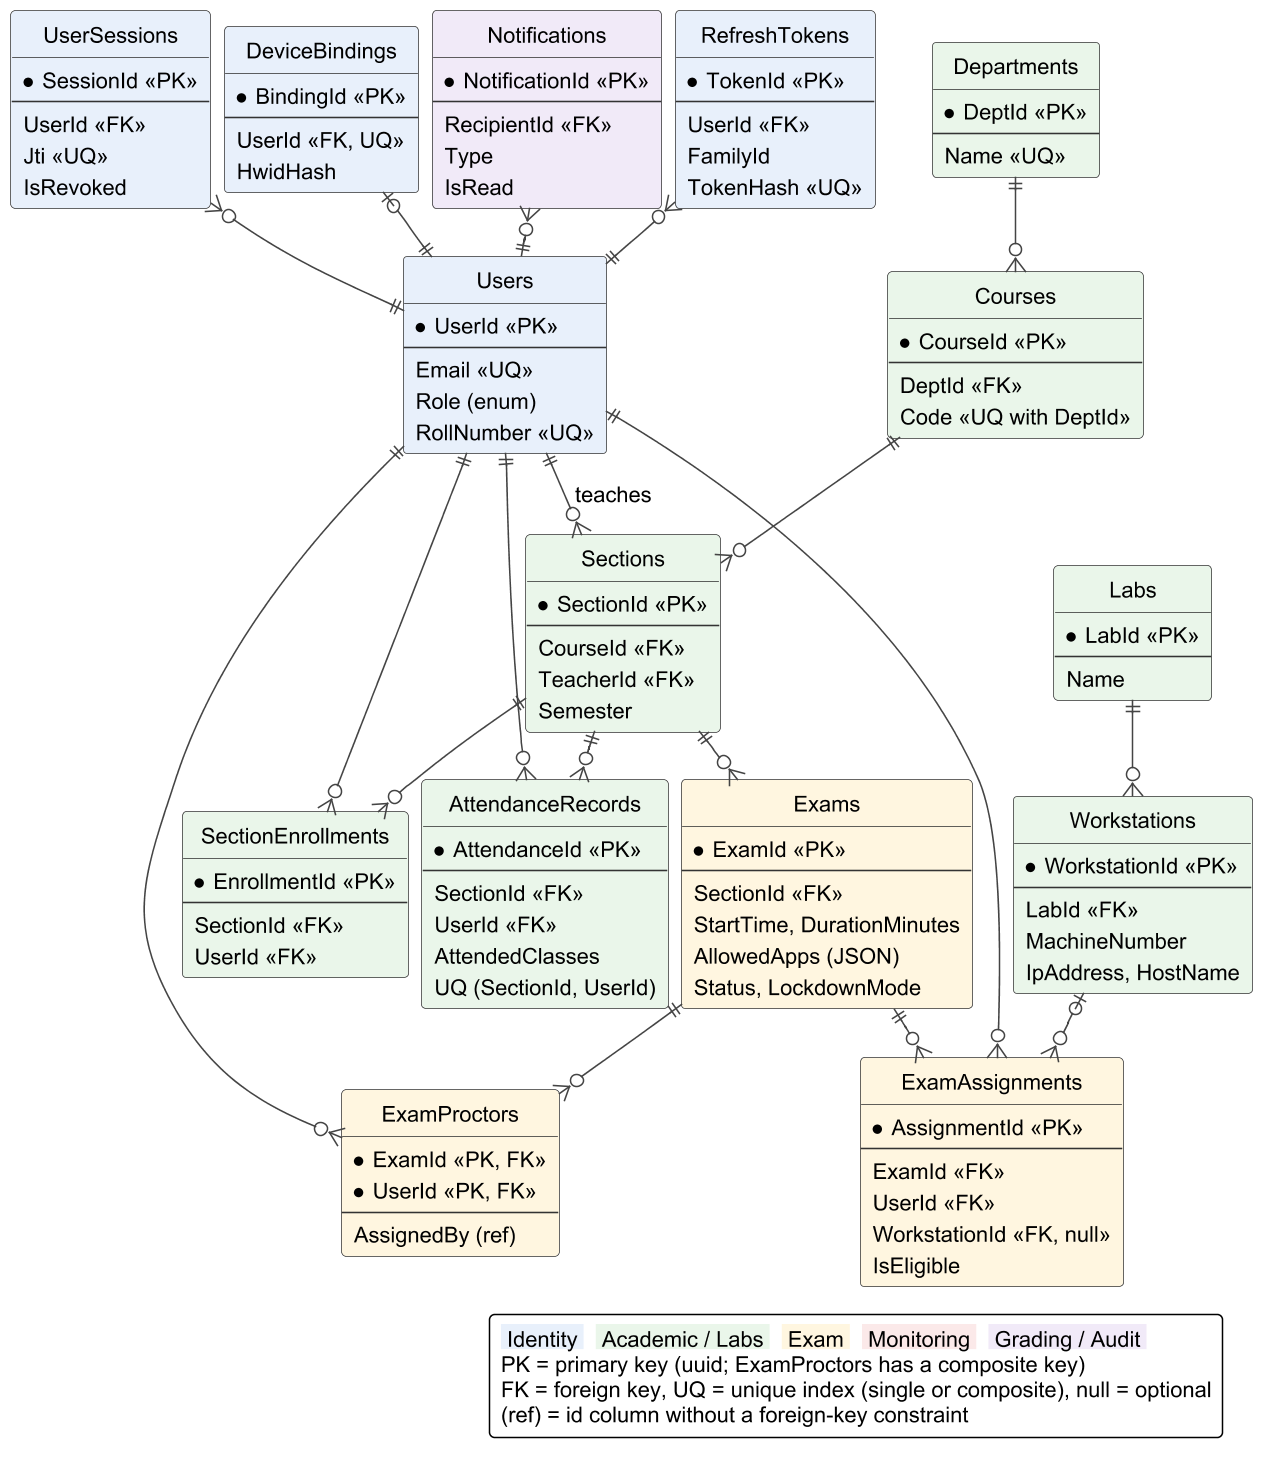
\includegraphics[width=\linewidth,height=0.9\textheight,keepaspectratio]{Figures/erd_diagram.png}
\caption{Entity Relationship Diagram of the SmartExam Database (a): Identity, Notifications, Academic Structure, Labs, Exams and Assignments}
\label{fig:erd_diagram}
\end{figure}

\begin{figure}[!htbp]
\centering
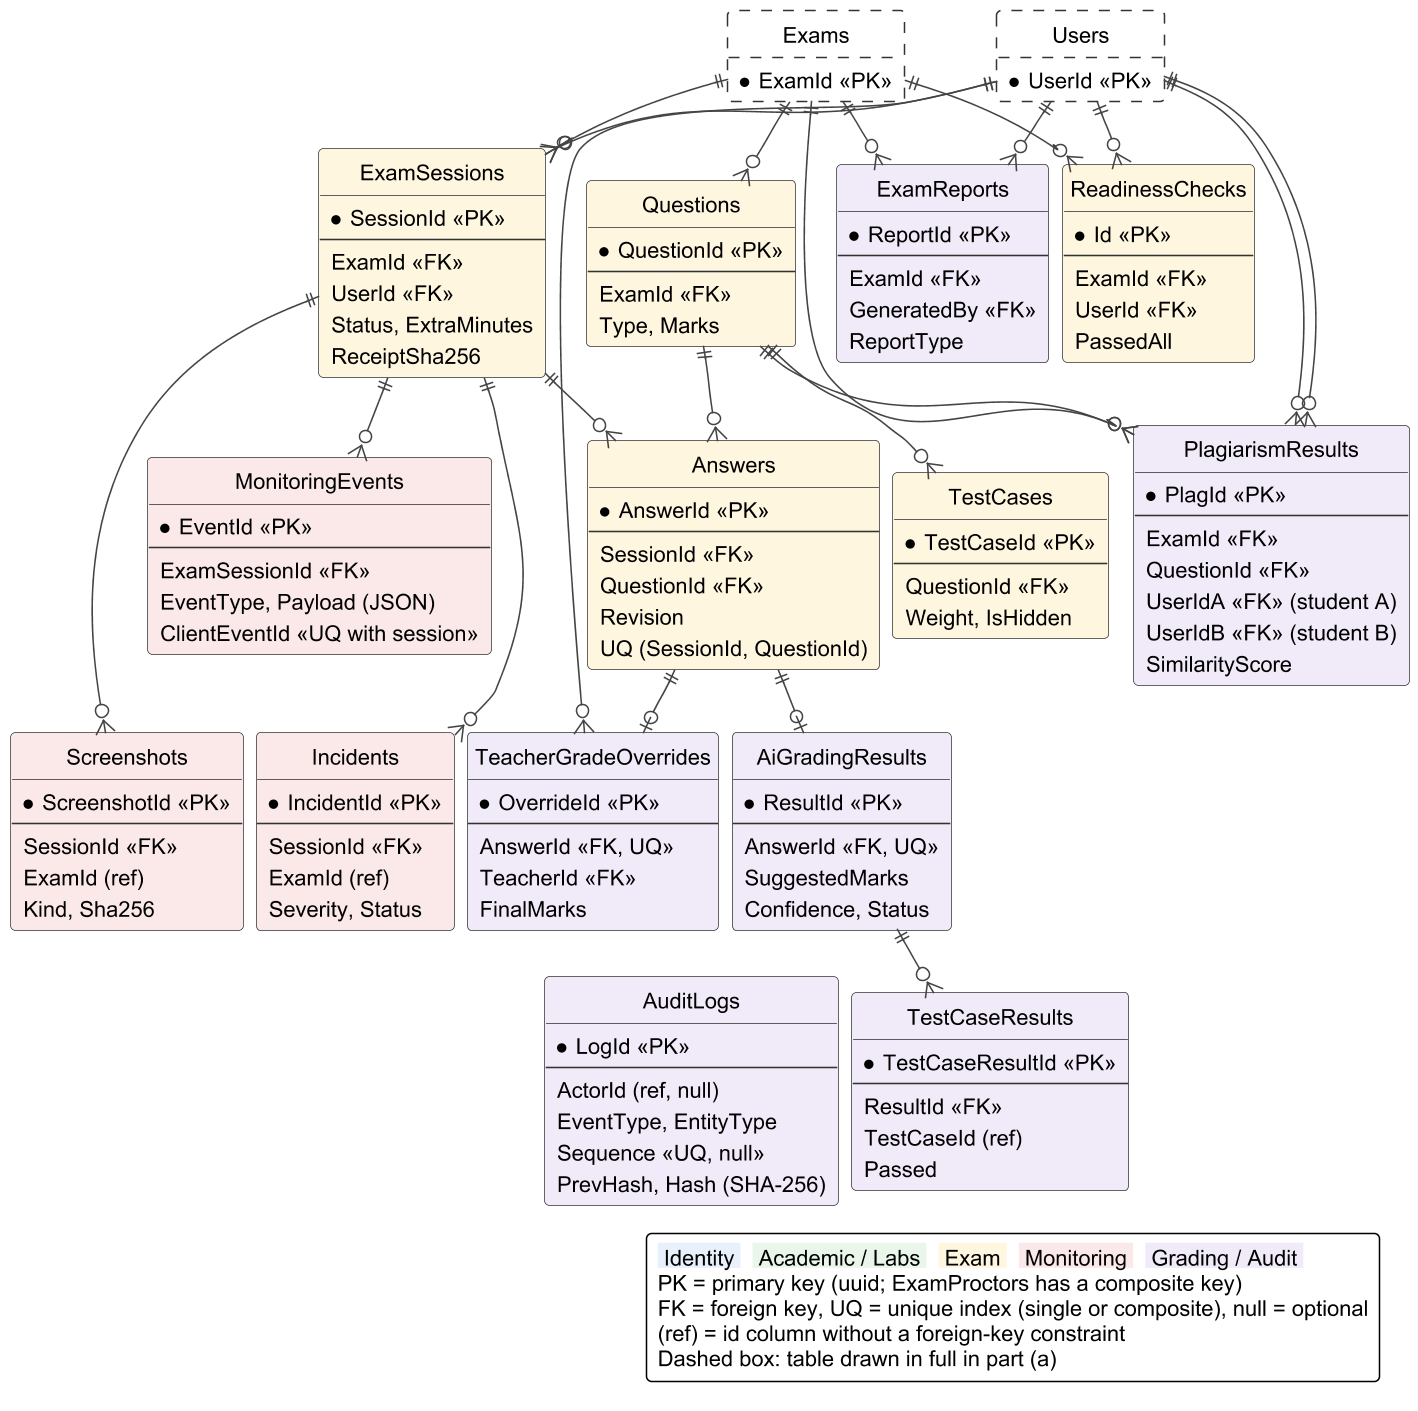
\includegraphics[width=\linewidth,height=0.9\textheight,keepaspectratio]{Figures/erd_diagram_b.png}
\caption{Entity Relationship Diagram of the SmartExam Database (b): Questions, Readiness, Exam Sessions, Monitoring, Grading, Reports and Audit}
\label{fig:erd_diagram_b}
\end{figure}

\texttt{AppDbContext} defines 29 tables. Table~\ref{tab:db_tables} groups them by module.

\begin{table}[!htb]
\centering
\caption{Database Tables by Module}
\label{tab:db_tables}
{\small\renewcommand{\arraystretch}{1.15}
\begin{tabularx}{\textwidth}{>{\raggedright\arraybackslash}p{3.2cm}>{\raggedright\arraybackslash}p{5.0cm}>{\raggedright\arraybackslash}X}
\hline\hline
\textbf{Group} & \textbf{Tables} & \textbf{Notes} \\
\hline\hline
Identity (M1, M7) & Users, DeviceBindings, UserSessions, RefreshTokens & Role is an enum column on \texttt{Users}; one binding per user (unique \texttt{UserId}). \\
Academic (M7, M9) & Departments, Courses, Sections, SectionEnrollments, AttendanceRecords & Attendance is unique per section and student. \\
Labs (M9) & Labs, Workstations & PC name and IP address used for seat checks. \\
Exams (M8--M10) & Exams, Questions, TestCases, ExamAssignments, ExamProctors & Allowed apps are a JSON column on \texttt{Exams}; assignments hold eligibility and the seat. \\
Exam run (M2, M3, M6) & ReadinessChecks, ExamSessions, Answers & Sessions hold status, extra minutes and the receipt hash; answers carry a revision. \\
Monitoring (M5, M10) & MonitoringEvents, Screenshots, Incidents & Events have a JSON payload and are unique per session and \texttt{ClientEventId}; screenshots store path, size and SHA-256; incidents hold the staff member's note, severity and status (Open, Escalated, Resolved). \\
Evaluation (M11) & AiGradingResults, TestCaseResults, TeacherGradeOverrides, PlagiarismResults & Suggested mark and confidence, per-test-case result, teacher override, and similarity per student pair. \\
Audit (M12) & AuditLogs, ExamReports, Notifications & Audit rows are hash-chained (\texttt{Sequence}, \texttt{PrevHash}, \texttt{Hash}); notifications also carry invigilator warnings. \\
\hline\hline
\end{tabularx}}
\end{table}

The main relationships are:
\begin{itemize}[nosep]
    \item \textbf{One-to-one:} a user has at most one \texttt{DeviceBinding}; an answer has at most one \texttt{AiGradingResult} and one \texttt{TeacherGradeOverride}.
    \item \textbf{One-to-many:} an exam has many questions, a question many test cases, and a session many answers, monitoring events and screenshots.
    \item \textbf{Junctions:} \texttt{ExamAssignments} links a student to an exam and an optional workstation; \texttt{ExamProctors} links invigilators to exams; \texttt{PlagiarismResults} links two students on one question.
\end{itemize}

\subsection{Data Flow Diagram}

The Data Flow Diagrams (DFDs) use the Yourdon/DeMarco notation: a circle is a process, a rectangle an external entity, a pair of horizontal lines a data store and a labelled arrow a data flow; a two-headed arrow means that the process reads and updates the store. A dashed circle is a process drawn in full in another figure, the dashed rectangle is the optional LLM grader, and an entity or store drawn twice to avoid crossing lines is marked *. The stores are named after the tables they hold: D1 identity (Users, DeviceBindings, UserSessions, RefreshTokens); D2 exams (Exams, Questions, TestCases); D3 academic, lab and assignment data (Departments, Courses, Sections, SectionEnrollments, Labs, Workstations, AttendanceRecords, ExamAssignments, ExamProctors); D4 sessions, answers and readiness checks; D5 monitoring evidence; D6 grading results and reports; D7 Notifications; D8 AuditLogs. All levels use the same numbers, and every flow of a process appears again in its decomposition.

As in the use-case diagram, the system is the whole of SmartExam: the desktop client with its lockdown, the web panel and the API. The student is the external entity, so the activity on the lab PC (applications, keys, USB drives, monitors), the screen and the webcam image enter the system as flows from the student. An Admin or SuperAdmin can also do everything a teacher can; those flows are drawn only from the Teacher.

\subsubsection{DFD Level 0}

Figure~\ref{fig:dfd_level_0} shows SmartExam as one process with its six external entities.

\begin{figure}[!htb]
\centering
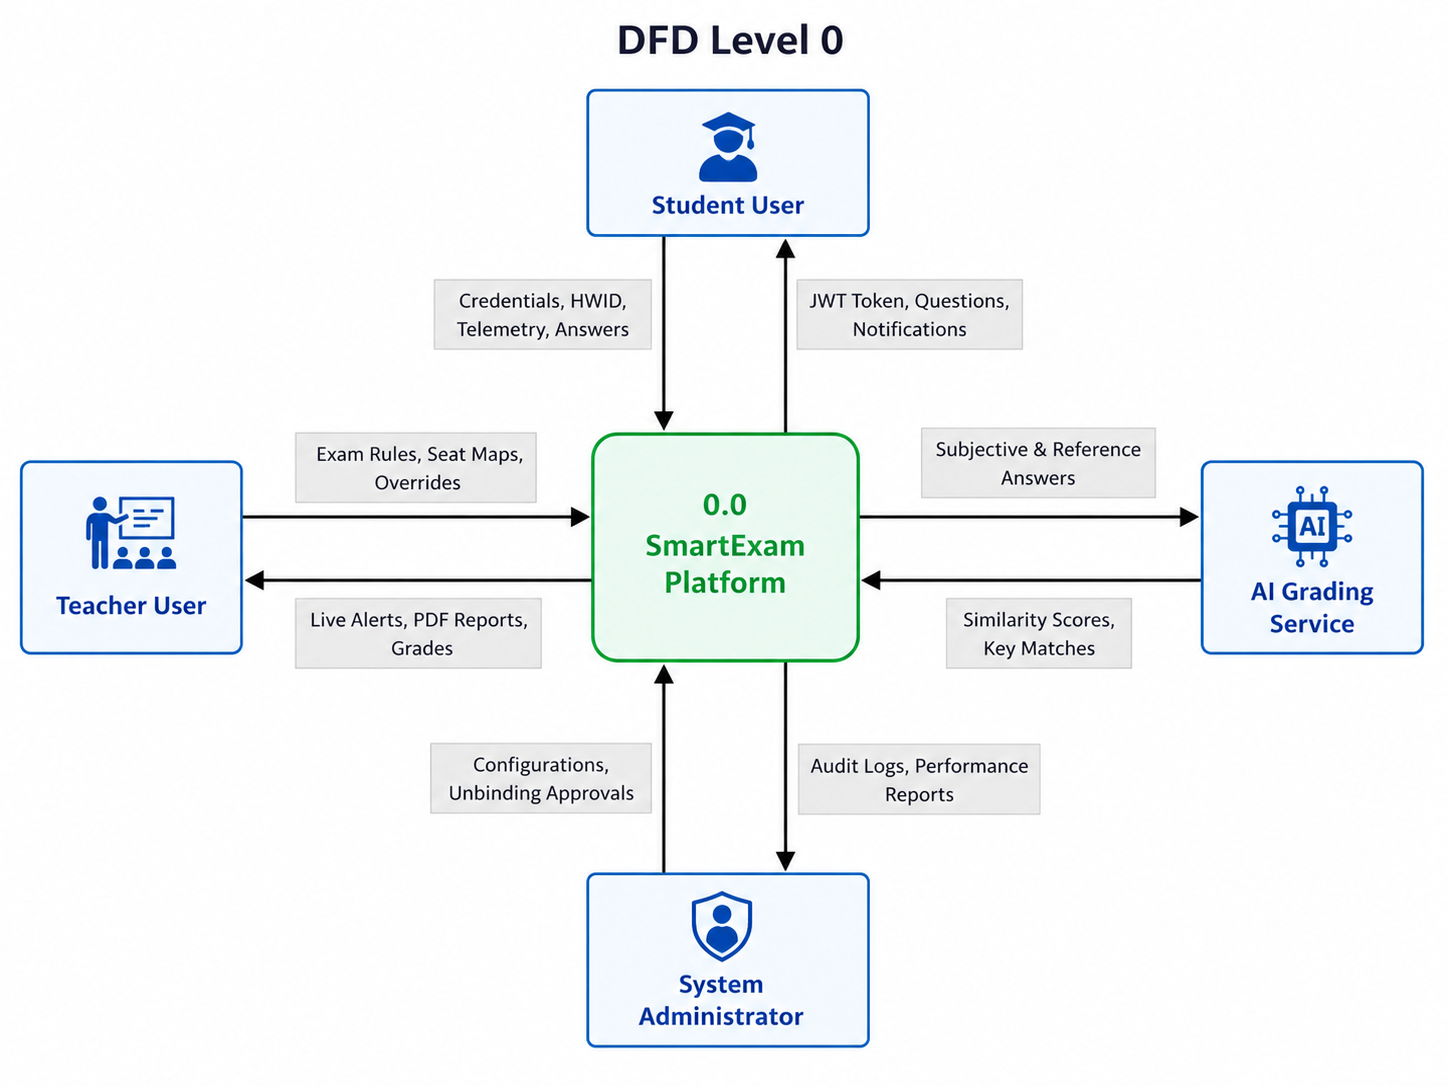
\includegraphics[width=\linewidth,height=0.9\textheight,keepaspectratio]{Figures/dfd_level_0.png}
\caption{DFD Level 0: Context Diagram}
\label{fig:dfd_level_0}
\end{figure}

\begin{itemize}[nosep]
    \item \textbf{Student:} sends credentials, the PC's hardware IDs, start, answers and submit, and is the source of the PC activity, screen and webcam image; receives the sign-in result, exam list, questions and receipt hash, the lockdown, warnings, extra time and unlocks, and on the web portal the results, violation history, performance and notifications.
    \item \textbf{Teacher and Invigilator:} the teacher sends exam settings, attendance, seats, invigilator assignments and announcements, accepts or overrides marks and requests reports; both send warnings, time extensions, unlocks, force-submits and incidents for the exams they supervise (the invigilator only for assigned exams) and receive live status over SignalR, and timelines and screenshots from the API on request. The teacher also receives suggested marks, the similarity matrix and the PDF, Excel and evidence-ZIP reports.
    \item \textbf{Admin/SuperAdmin:} sends user, role, device-binding, department, course, lab and workstation changes; receives the audit log with its hash-chain status and system analytics.
    \item \textbf{Email server (SMTP):} receives exam schedule, grade and announcement emails.
    \item \textbf{LLM grader (Groq or Gemini, optional, off by default):} receives theory answers with the model answer and rubric keywords, and code test results; returns a suggested mark or a code summary.
\end{itemize}

\subsubsection{DFD Level 1}

Level 1 has five processes. To keep its labels legible it is drawn on two landscape pages that share the stores: Figure~\ref{fig:dfd_level_1} holds 1.0--3.0 and Figure~\ref{fig:dfd_level_1b} holds 4.0 and 5.0, and the dashed circles show the flows between the two parts.

\begin{sidewaysfigure}
\centering
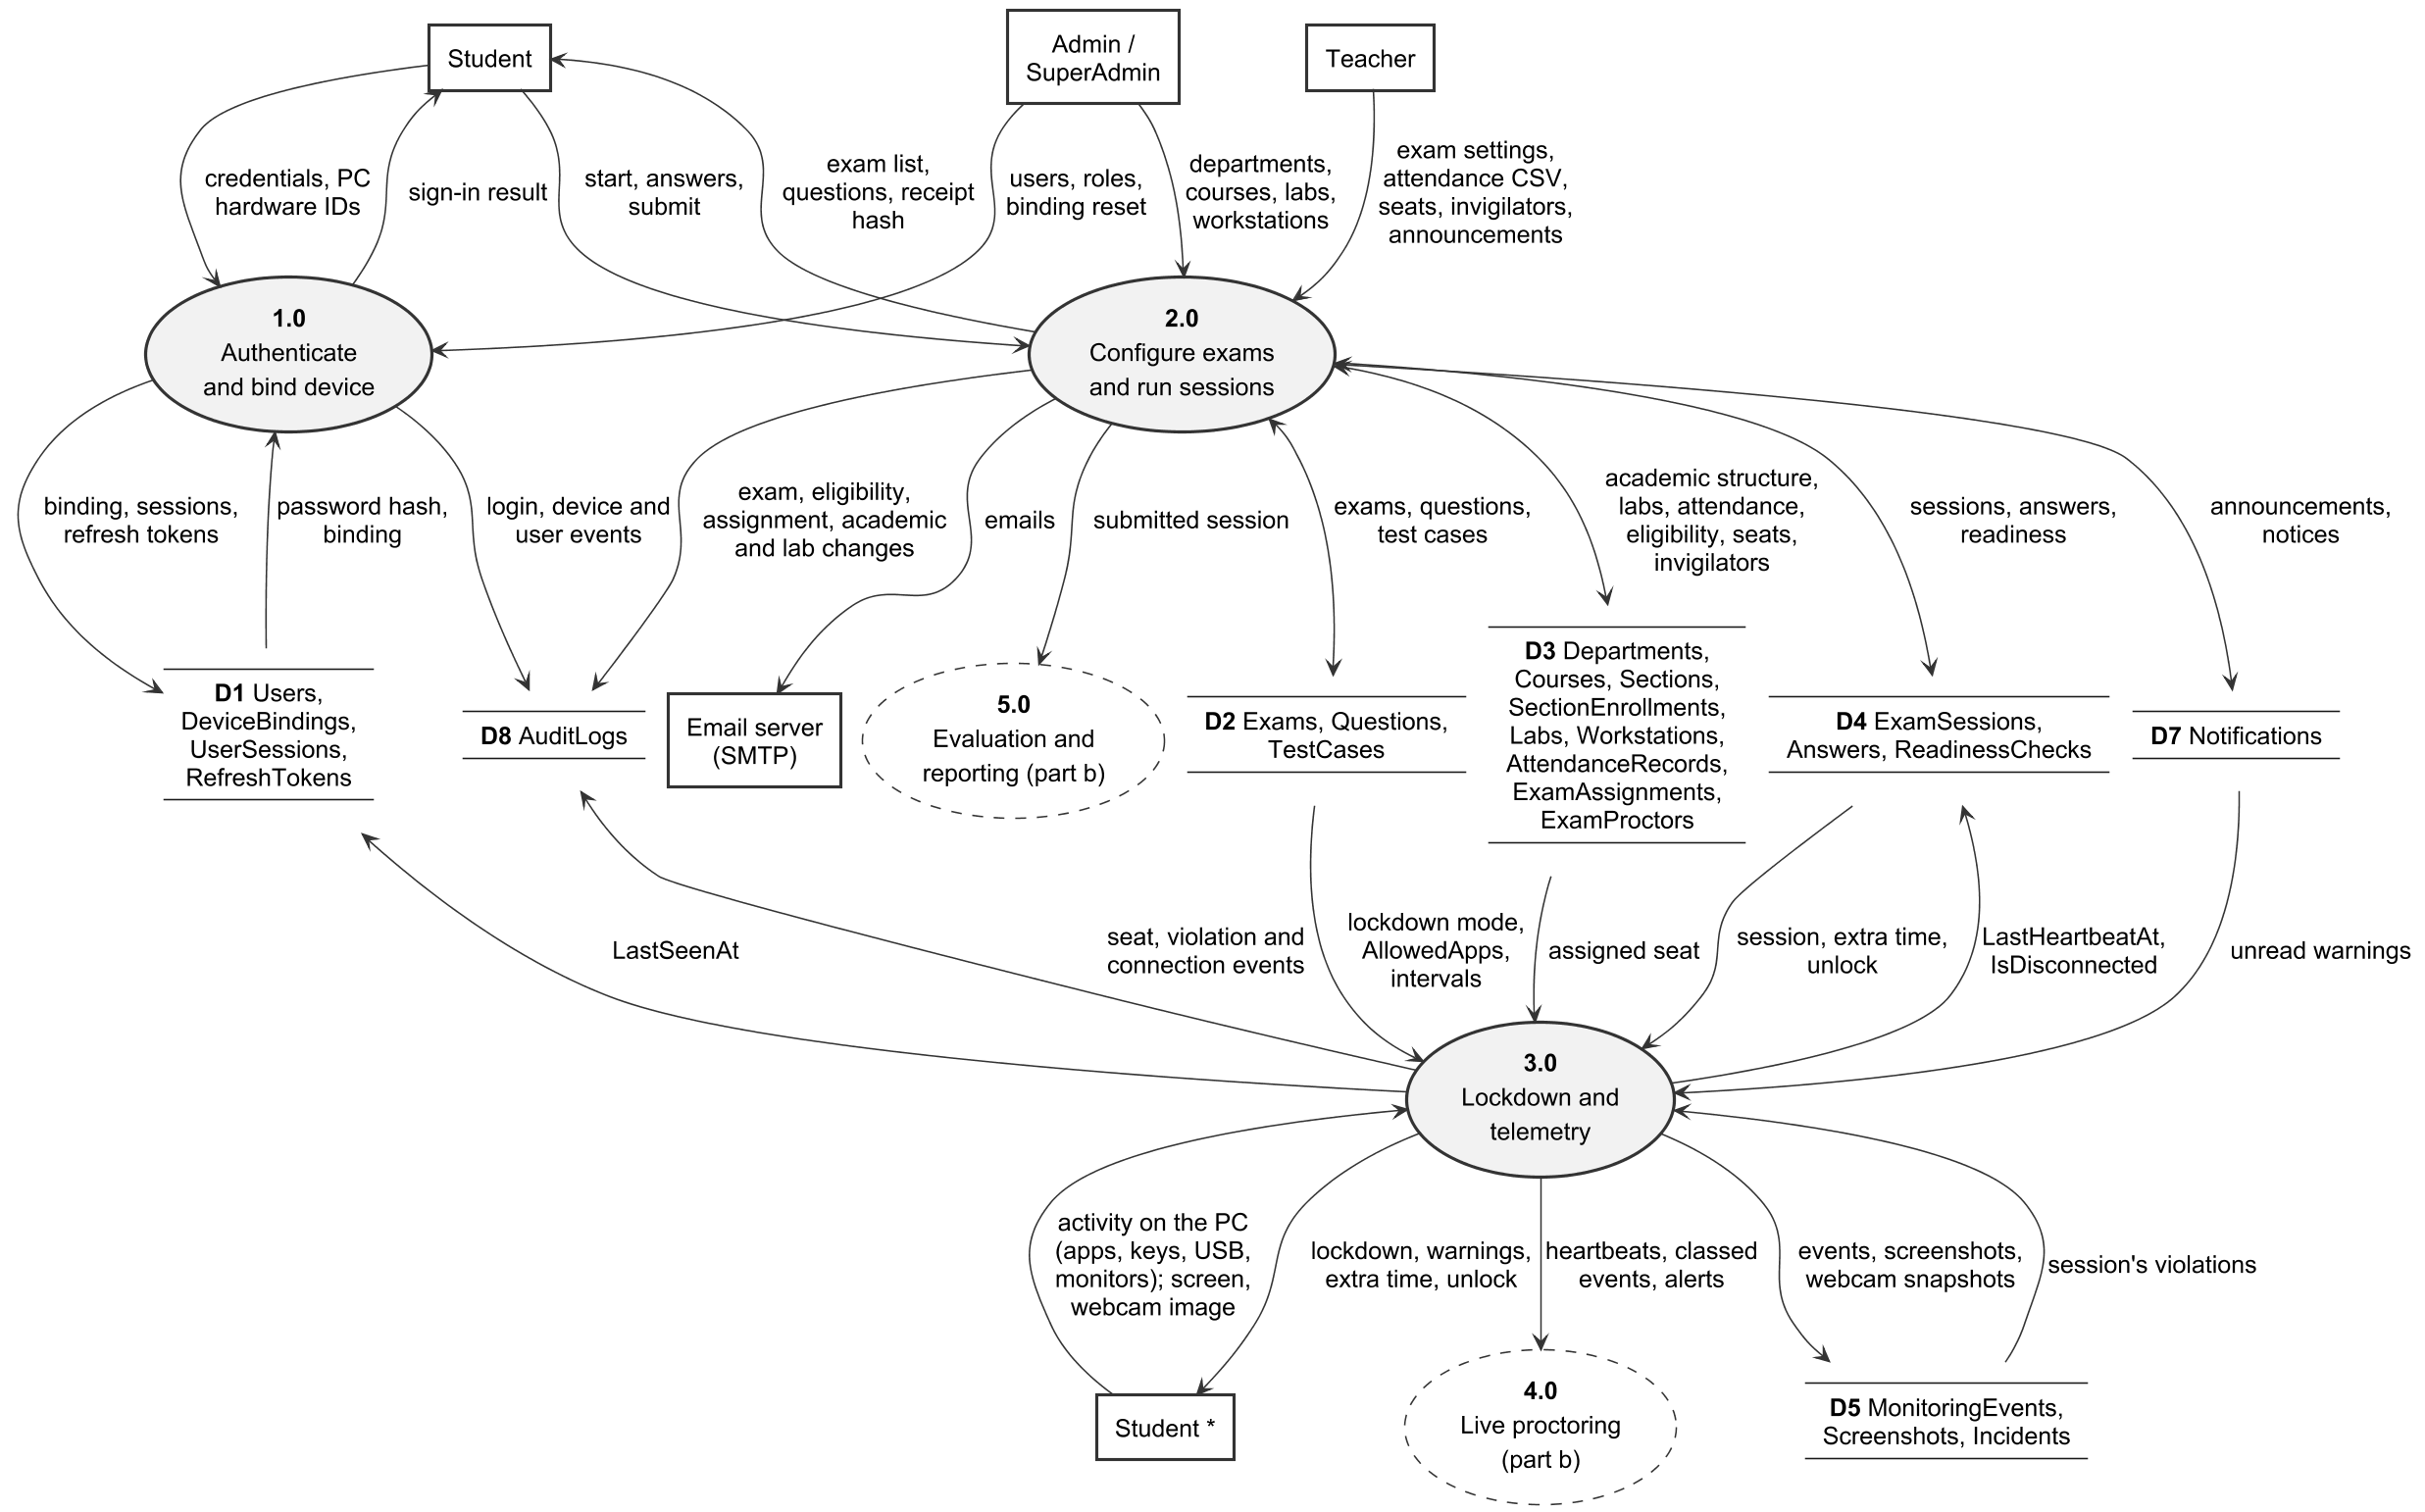
\includegraphics[width=\linewidth,height=415pt,keepaspectratio]{Figures/dfd_level_1.png}
\caption{DFD Level 1 (a): Sign-in, Exam Set-up and Exam Session (Processes 1.0--3.0)}
\label{fig:dfd_level_1}
\end{sidewaysfigure}

\begin{sidewaysfigure}
\centering
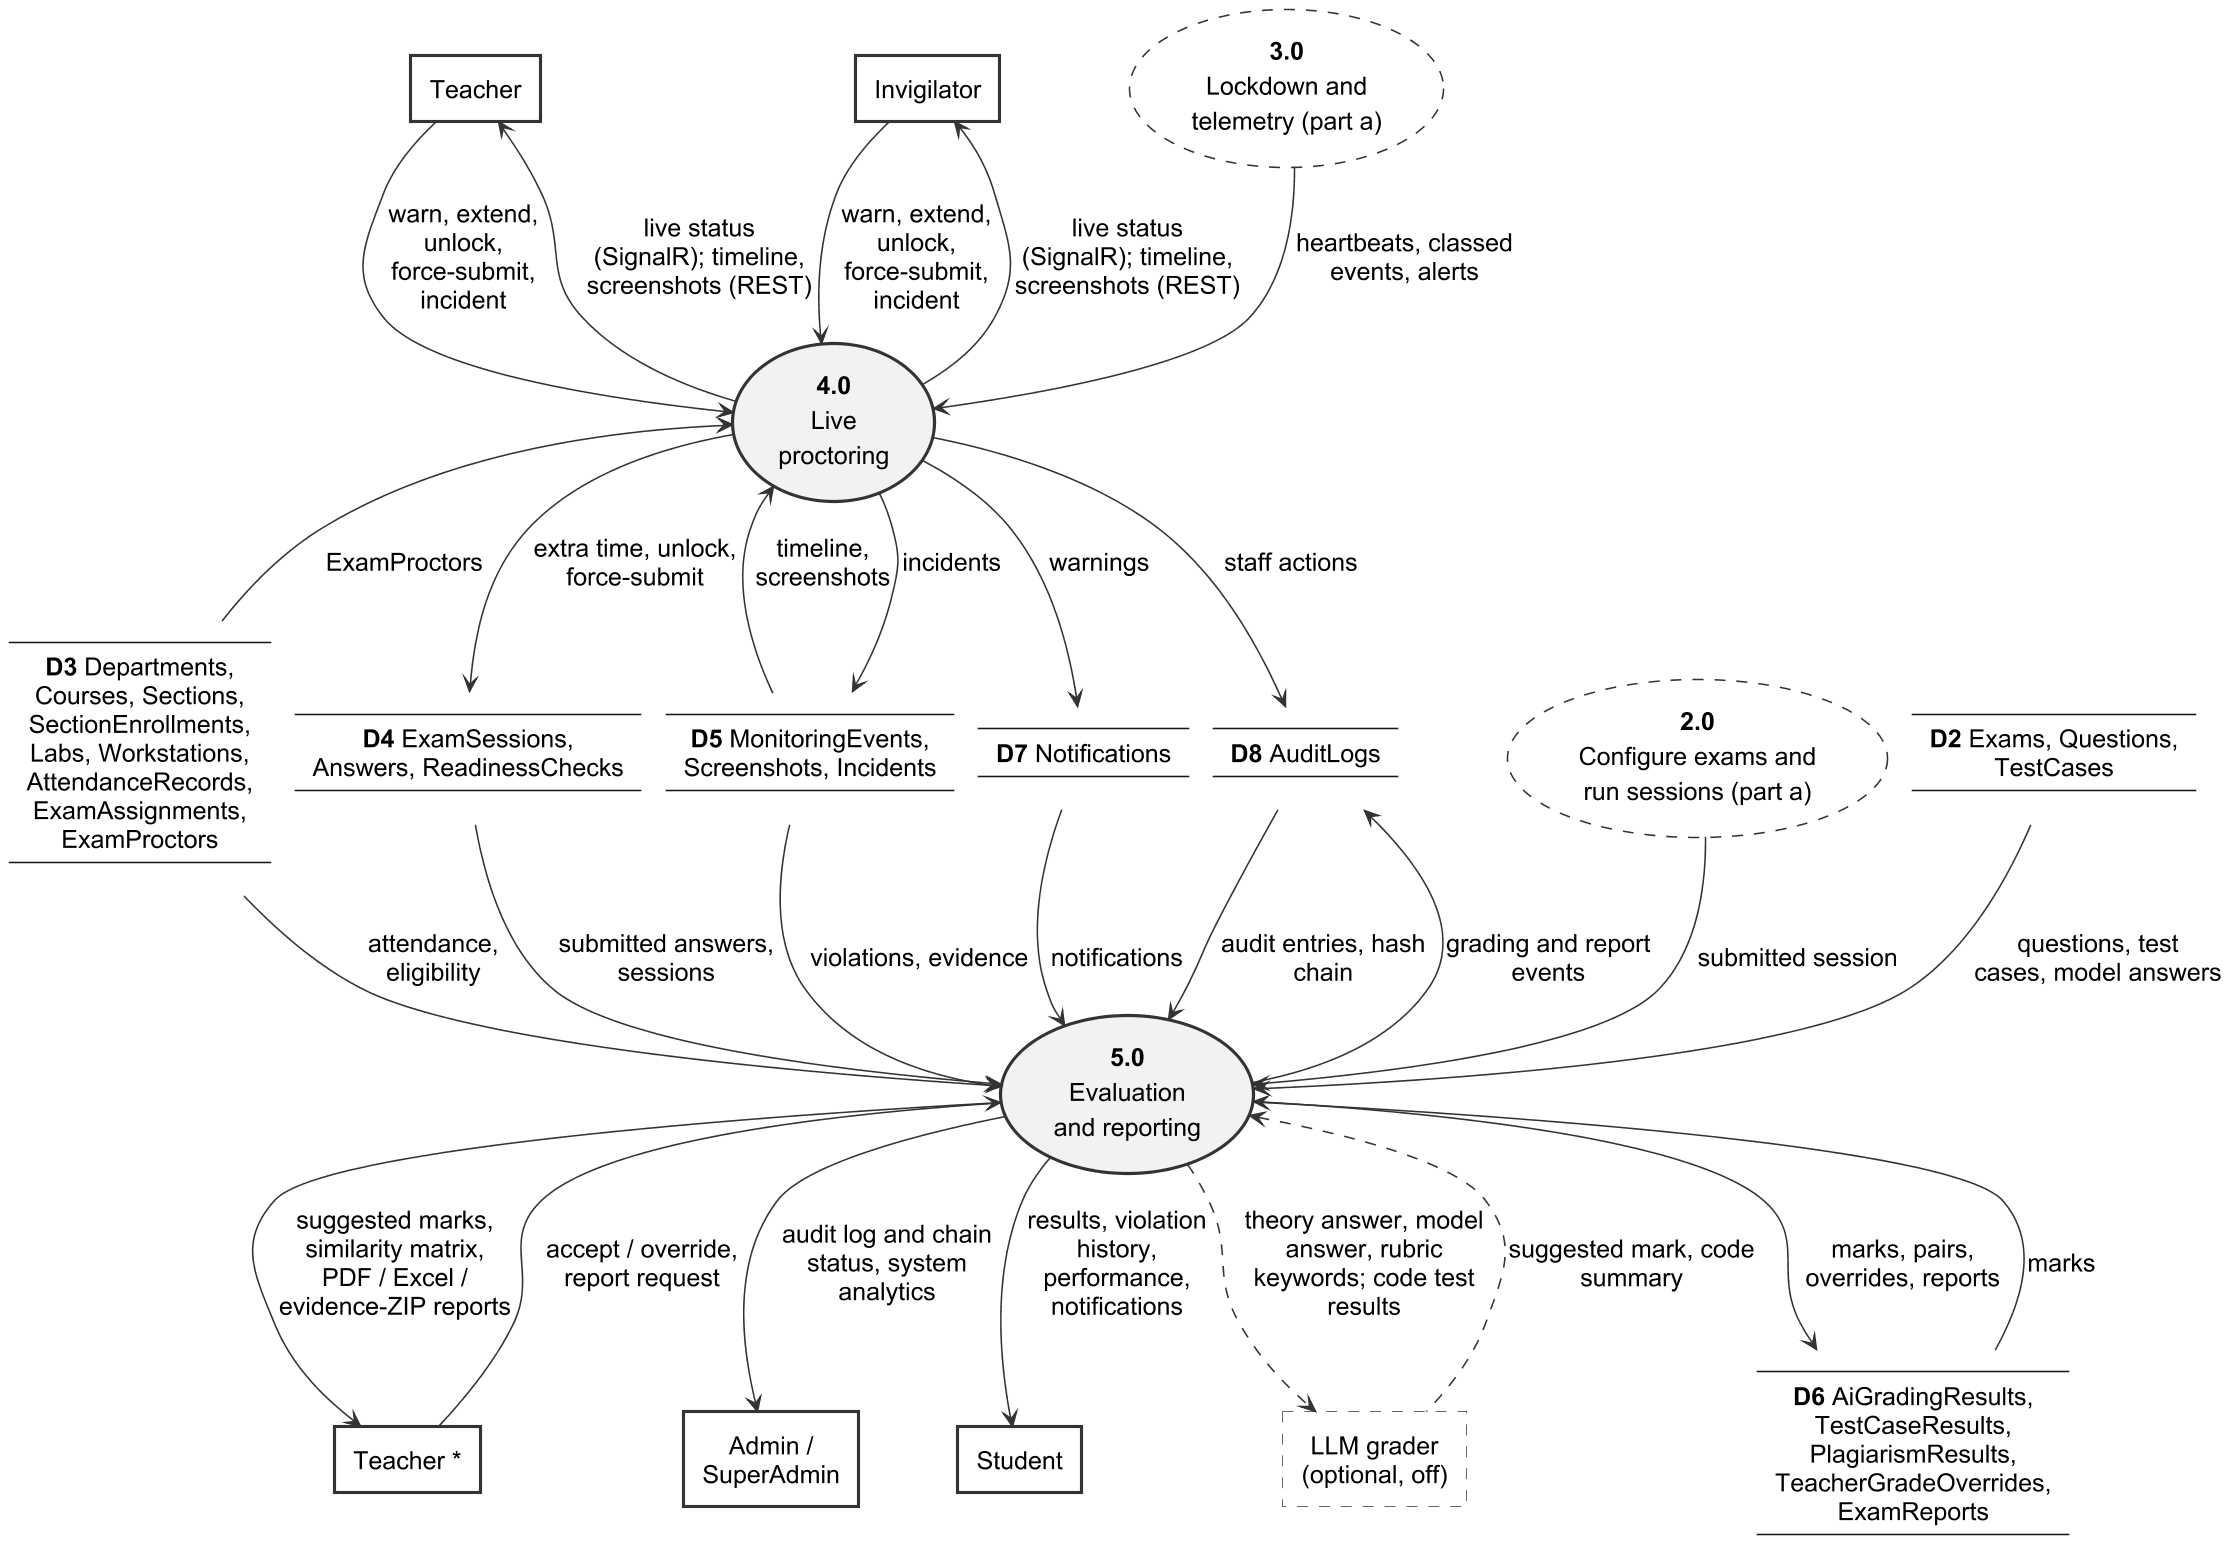
\includegraphics[width=\linewidth,height=415pt,keepaspectratio]{Figures/dfd_level_1b.png}
\caption{DFD Level 1 (b): Live Proctoring and Evaluation (Processes 4.0 and 5.0)}
\label{fig:dfd_level_1b}
\end{sidewaysfigure}

\begin{sloppypar}
\begin{enumerate}[nosep]
    \item \textbf{1.0 Authenticate and bind device:} reads the password hash and device binding from D1, writes the binding, sessions and refresh tokens, and audits login, device and user events in D8. Admin user, role and binding-reset changes enter here.
    \item \textbf{2.0 Configure exams and run sessions:} stores exams, questions and test cases (D2), departments, courses, labs and workstations, attendance, eligibility, seats and invigilator assignments (D3), and sessions, answers and readiness results (D4); writes announcements and schedule and grade notices to D7 and sends them as emails; audits exam, eligibility, assignment, academic-structure and lab changes in D8; and passes each submitted session to 5.0.
    \item \textbf{3.0 Lockdown and telemetry:} the client applies the exam's lockdown mode and allowed apps (D2) to the PC and sends heartbeats, event batches, screenshots and webcam snapshots. The API checks the assigned seat (D3), reads the session's violations (D5) for the live tile status, and returns the session's extra time and unlock (D4) and unread warnings (D7) in the heartbeat reply. It writes events and captures to D5, \texttt{LastHeartbeatAt} and the disconnected flag to D4, \texttt{LastSeenAt} to D1 and seat, violation and connection events to D8, and passes heartbeats, classed events and alerts to 4.0.
    \item \textbf{4.0 Live proctoring:} checks \texttt{ExamProctors} (D3), pushes live status to teachers and invigilators over SignalR, serves timelines and screenshots (D5) on request over REST, and stores their warnings (D7), extra time, unlocks and force-submits (D4), incidents (D5) and an audit entry for each action (D8).
    \item \textbf{5.0 Evaluation and reporting:} grades submitted answers (calling the LLM only if enabled), compares submissions within an exam, stores marks, similarity pairs, overrides and reports (D6), builds reports from D3--D6 and D8, audits grading and report events in D8, and serves the audit log, analytics and student results.
\end{enumerate}
\end{sloppypar}

\DiagramBarrier
\subsubsection{DFD Level 2}

Level 2 expands processes 3.0 and 5.0 with the same stores as level 1; each is drawn in two parts, and a dashed circle stands for the process in the other part.

\begin{sloppypar}
\begin{enumerate}[nosep]
    \item \textbf{3.1--3.5 Lockdown and telemetry (Figures~\ref{fig:dfd_level_2} and~\ref{fig:dfd_level_2_api}):} on the lab PC, 3.1 enforces the lockdown with \texttt{ProcessGuardService}, the keyboard hook and the USB, monitor, remote-session and VM guards, reports each breach as an event, and relaxes the lock while an unlock from the heartbeat reply is valid. 3.2 runs the webcam checks, takes screenshots and webcam snapshots, spools events, sends a heartbeat every 10~s and event batches every 5~s, and shows the warnings, extra time and remaining time from the reply. In the API, \texttt{MonitoringController} receives the uploads, checks the seat with \texttt{SeatGuard} and builds the reply (3.3). 3.4 updates \texttt{LastHeartbeatAt} and \texttt{LastSeenAt}, stores a heartbeat event when something changed or at least every 60~s, sets the tile status from the session's violations, and lets the watchdog mark a student silent for 30~s as disconnected. \texttt{ViolationClassifier} gives each event its type and severity (Warning, Suspicious or Violation); events are saved, de-duplicated by \texttt{ClientEventId}, and violations are pushed as \texttt{ViolationEvent} (3.5). Seat mismatches, violations, disconnects and reconnects are audited.
\end{enumerate}
\end{sloppypar}

\begin{figure}[!htbp]
\centering
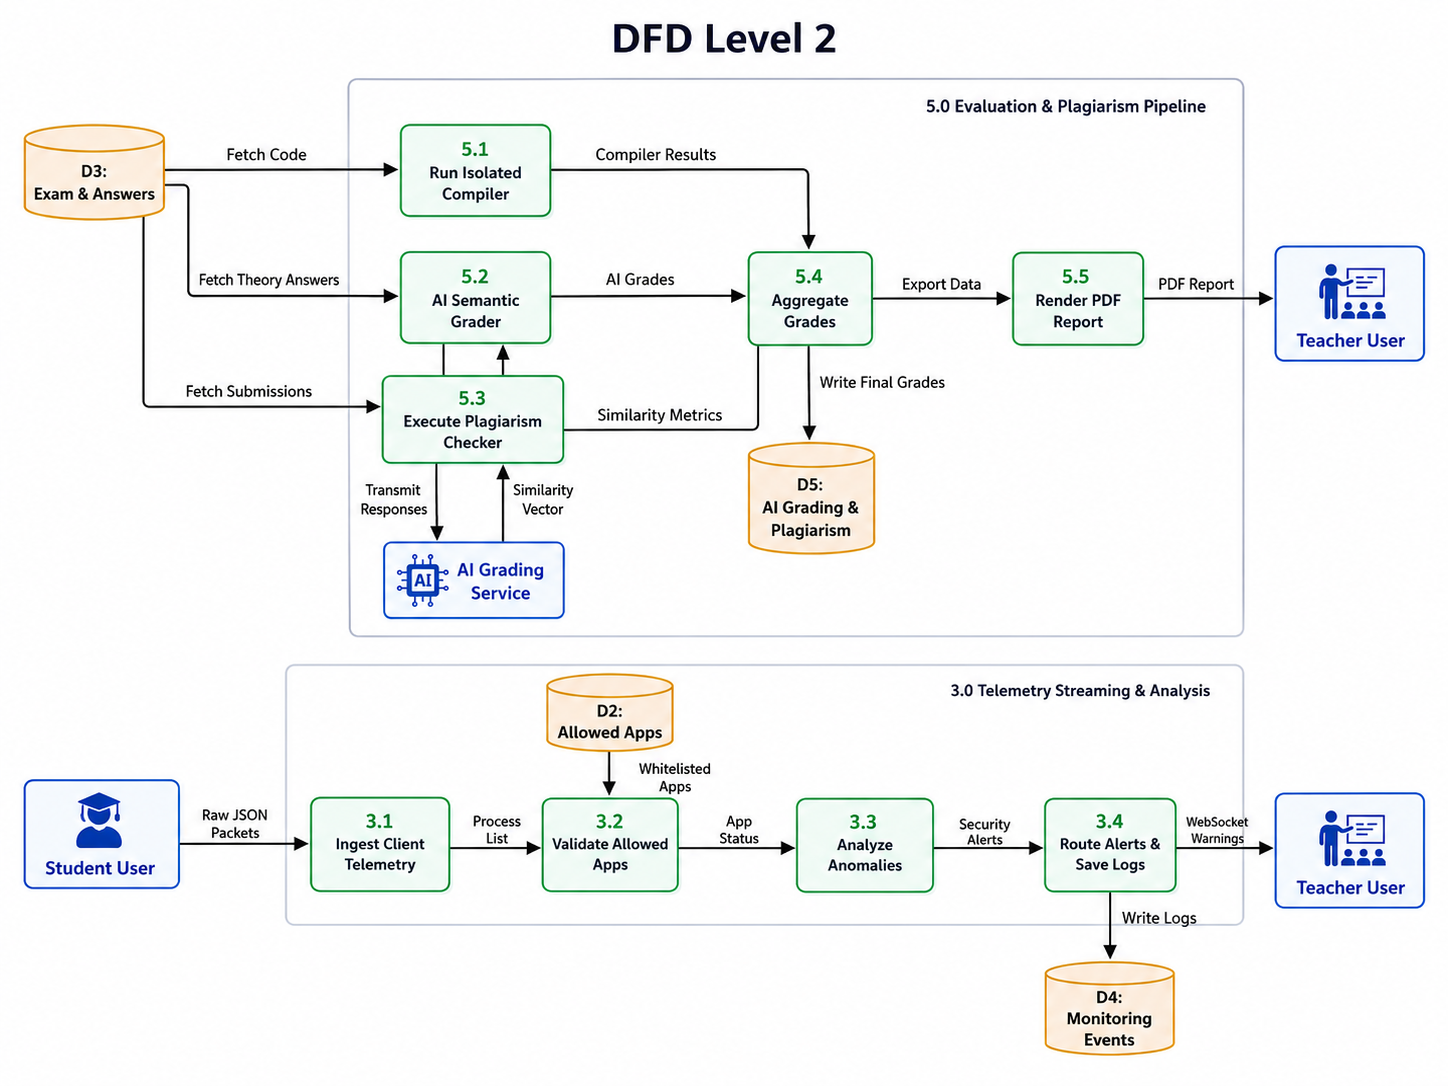
\includegraphics[width=\linewidth,height=0.9\textheight,keepaspectratio]{Figures/dfd_level_2.png}
\caption{DFD Level 2 of Process 3.0 (a): Client Side, Processes 3.1 and 3.2}
\label{fig:dfd_level_2}
\end{figure}

\begin{sloppypar}
\begin{enumerate}[nosep,start=2]
    \item \textbf{5.1--5.6 Evaluation and reporting (Figures~\ref{fig:dfd_level_2b} and~\ref{fig:dfd_level_2b_reports}):} grading runs only when the exam has AI evaluation enabled, and practice exams are not compared. The code runner tests each C or C++ answer against its test cases (5.1); MCQs are scored by key and theory answers by TF-IDF, or by the optional LLM (5.2); k-gram winnowing compares answers pairwise within the exam (5.3). Suggested marks, similarity pairs and the teacher's accept or override decisions are saved and audited (5.4). On request, 5.5 builds the exam summary PDF, the attendance, violations and scores PDFs (QuestPDF), the Excel workbook and the evidence ZIP, lists each file in \texttt{ExamReports} and audits each export except the summary PDF as \texttt{REPORT\_GENERATED} with the file's SHA-256. 5.6 serves the audit log and its hash-chain check (valid, or the first broken row), system analytics, and each student's results, violation history, performance and notifications.
\end{enumerate}
\end{sloppypar}

\begin{sidewaysfigure}
\centering
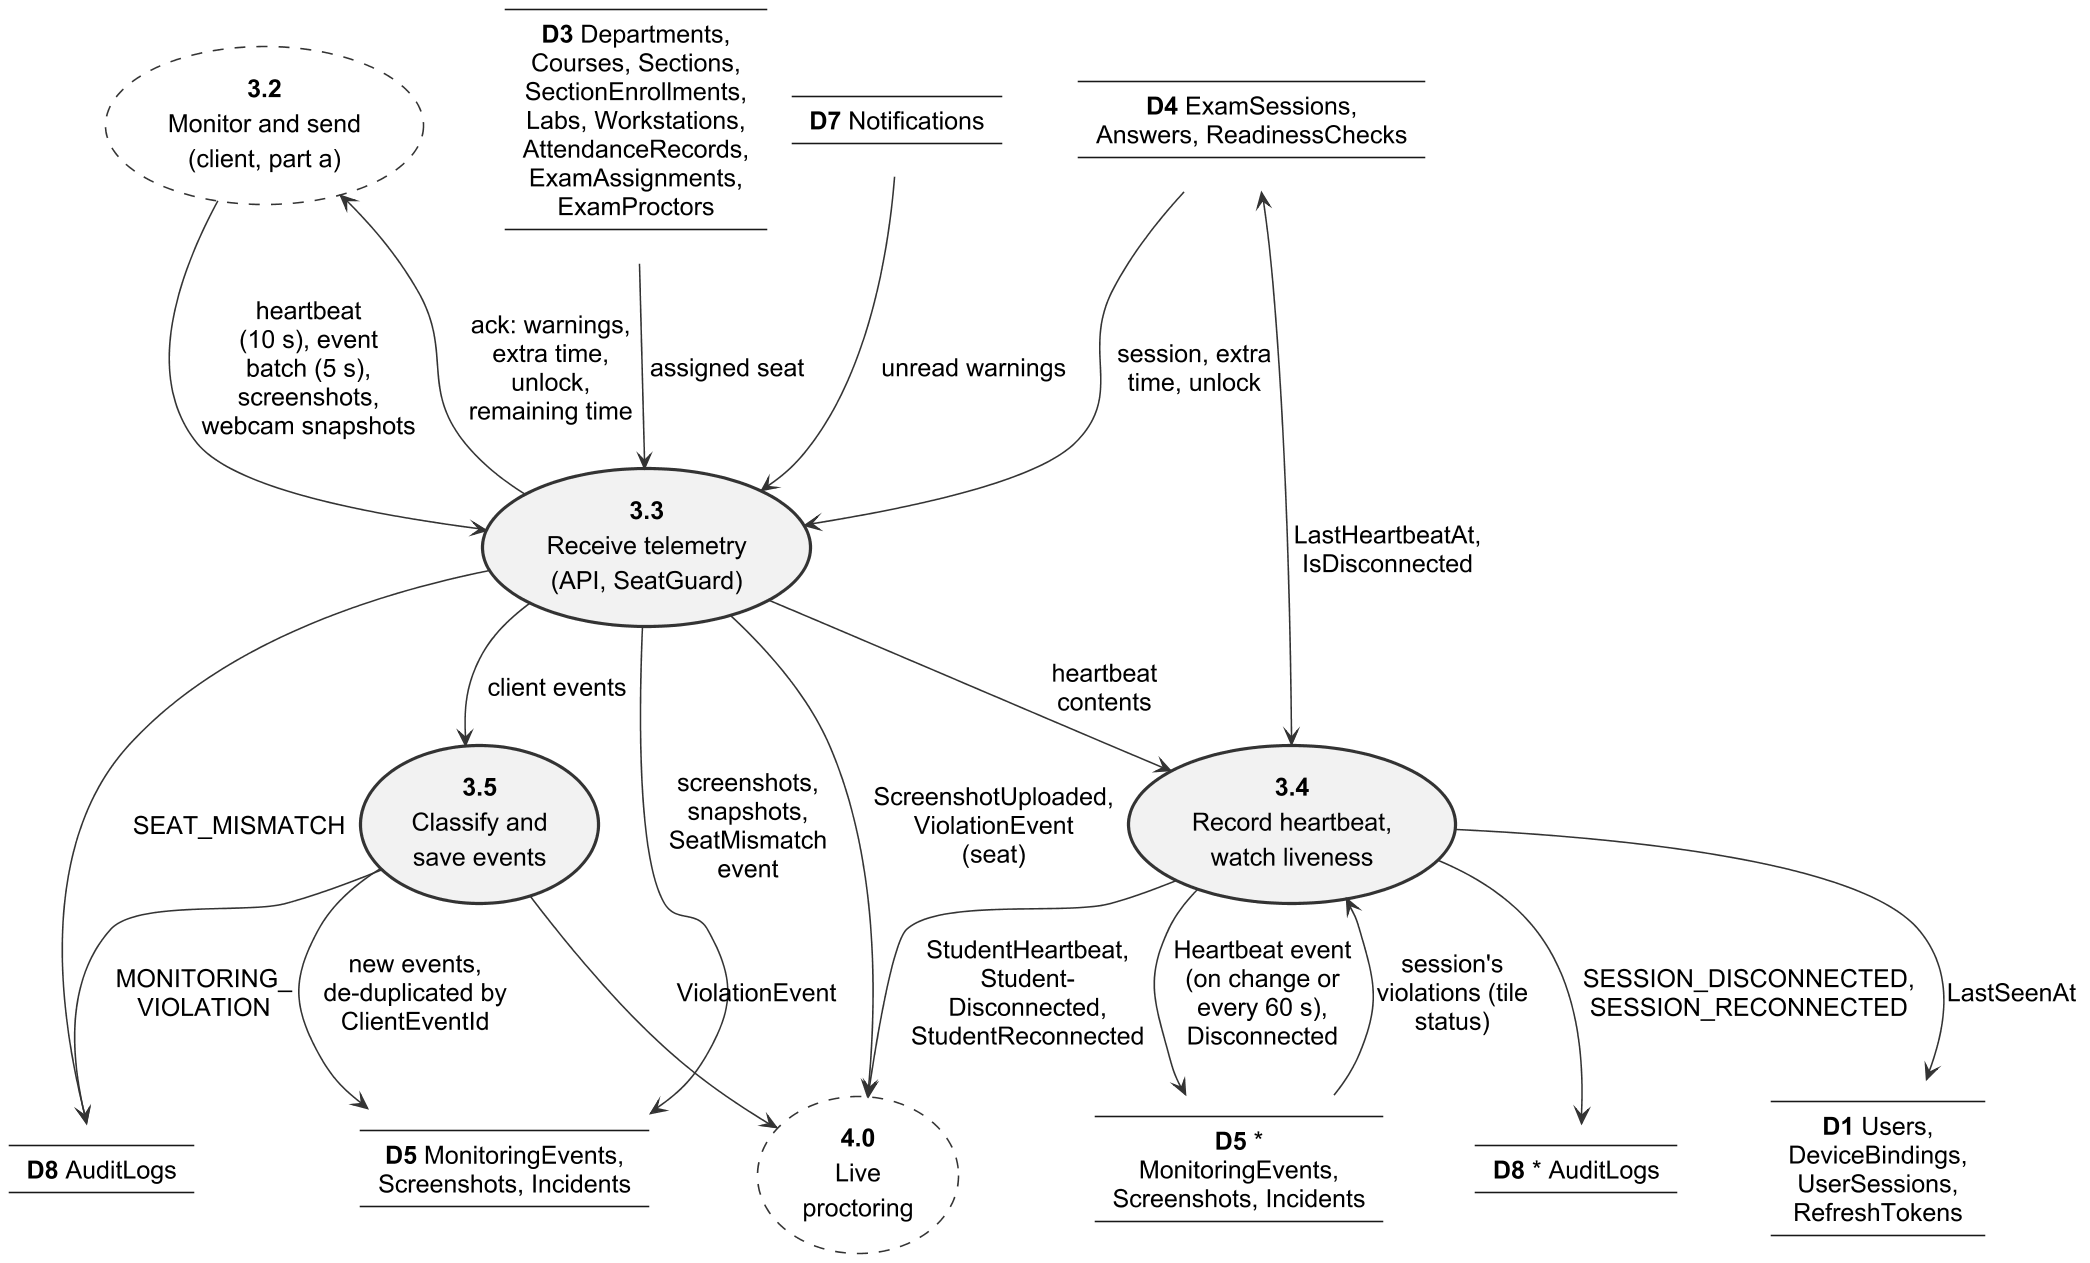
\includegraphics[width=\linewidth,height=415pt,keepaspectratio]{Figures/dfd_level_2_api.png}
\caption{DFD Level 2 of Process 3.0 (b): API Side, Processes 3.3--3.5}
\label{fig:dfd_level_2_api}
\end{sidewaysfigure}

\begin{sidewaysfigure}
\centering
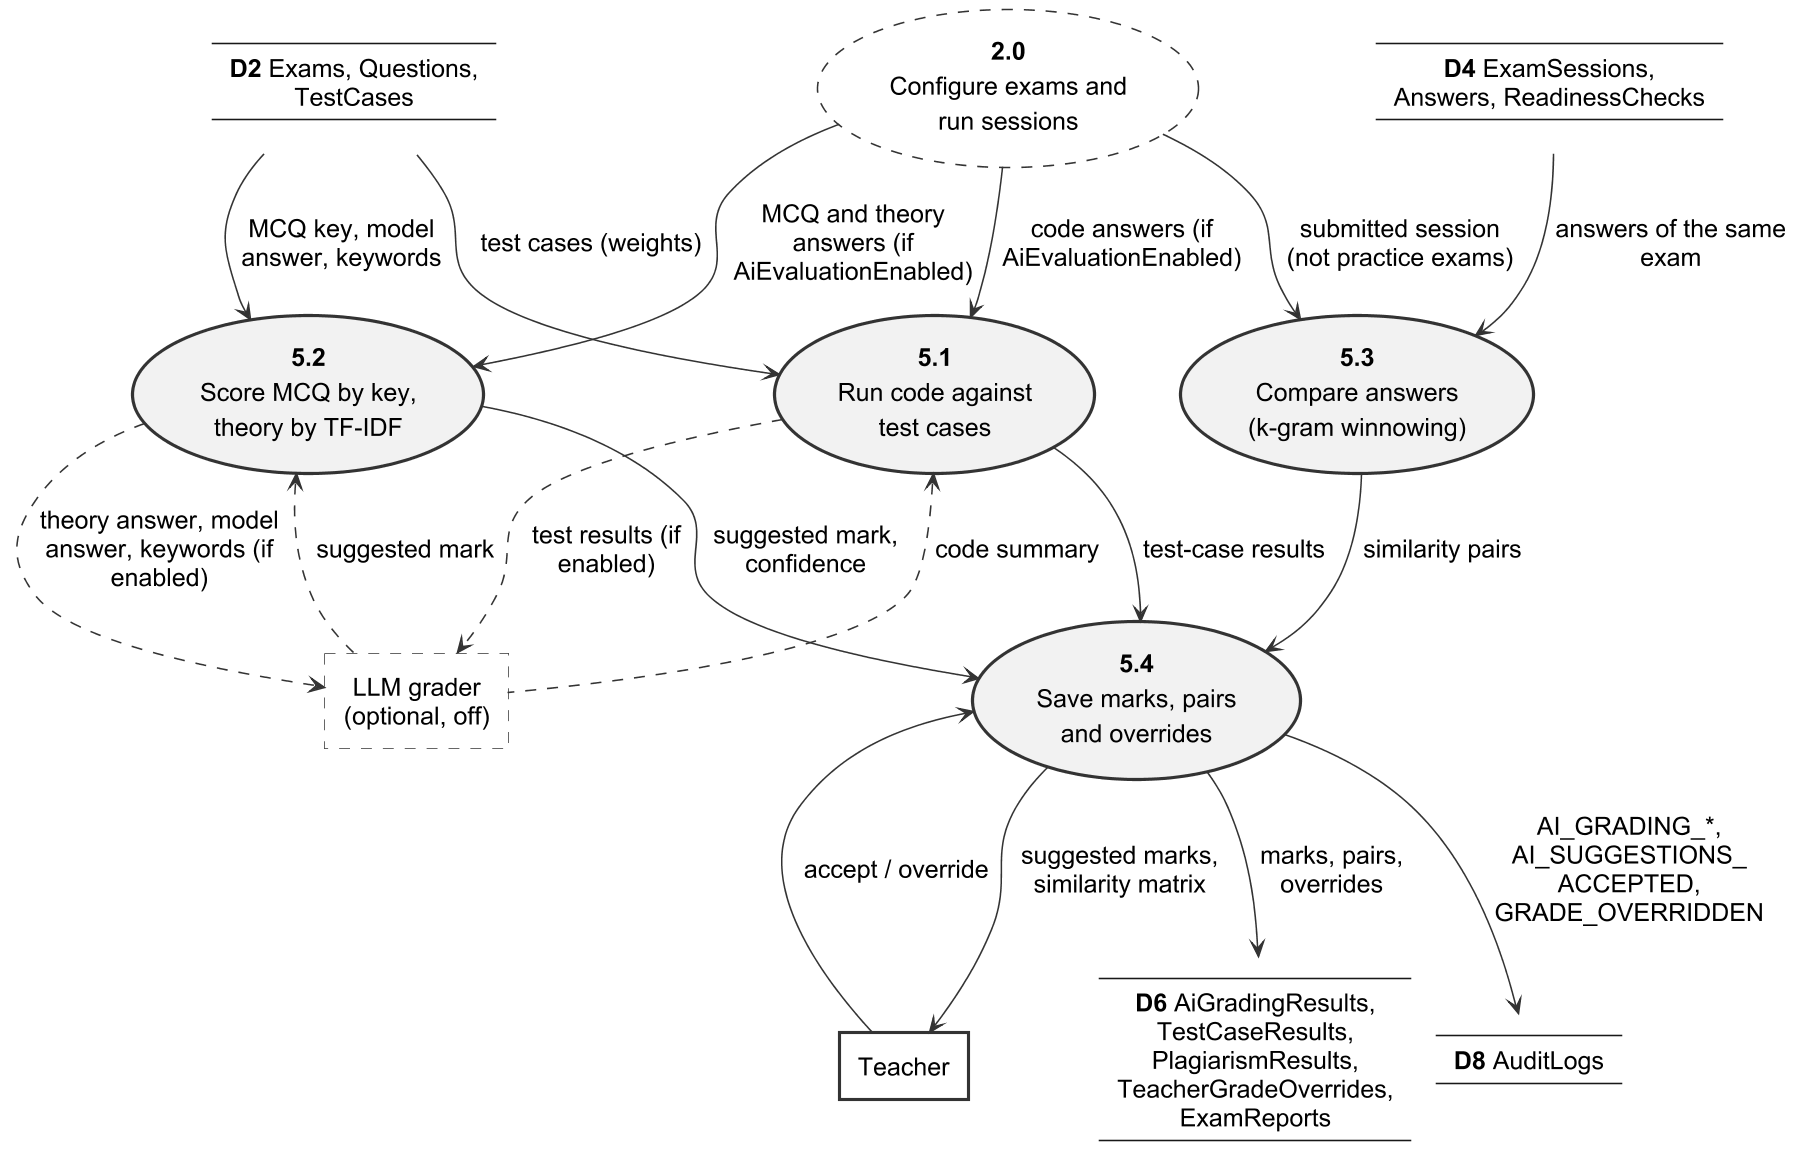
\includegraphics[width=\linewidth,height=415pt,keepaspectratio]{Figures/dfd_level_2b.png}
\caption{DFD Level 2 of Process 5.0 (a): Grading, Processes 5.1--5.4}
\label{fig:dfd_level_2b}
\end{sidewaysfigure}

\begin{sidewaysfigure}
\centering
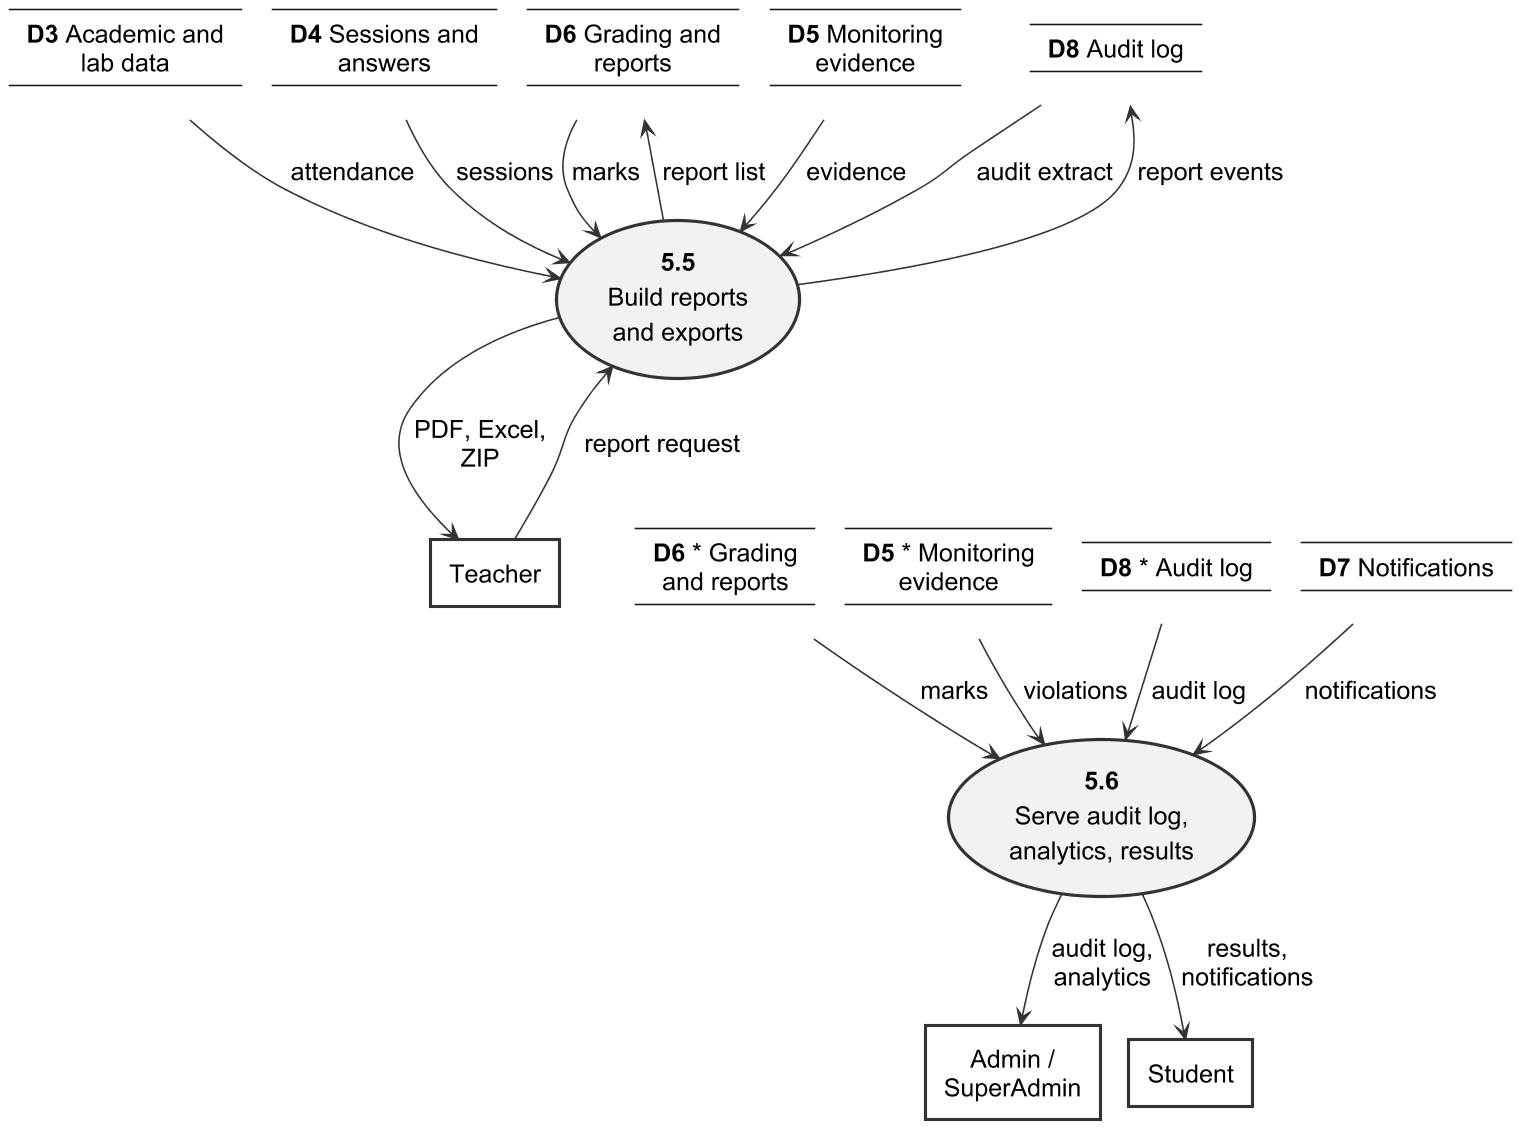
\includegraphics[width=\linewidth,height=415pt,keepaspectratio]{Figures/dfd_level_2b_reports.png}
\caption{DFD Level 2 of Process 5.0 (b): Reports and Read-only Services, Processes 5.5 and 5.6}
\label{fig:dfd_level_2b_reports}
\end{sidewaysfigure}

\chapter{SYSTEM DESIGN}
\label{chap:system_design}
% Each diagram is its own float, sized so its smallest text prints at 6.5 pt or more;
% \DiagramBarrier (defined in FYP-Final.tex) keeps each paragraph next to its figures.
\renewcommand{\floatpagefraction}{0.7}
\renewcommand{\topfraction}{0.9}
\renewcommand{\textfraction}{0.1}

SmartExam has three parts: the WPF \texttt{Student\_Desktop\_App} on the lab workstations, the React \texttt{Admin\_Web\_Panel} for staff and students, and the ASP.NET Core \texttt{Backend\_API}, which keeps its data in PostgreSQL. Section~\ref{sec:structure_diagrams} gives their static structure in class, deployment and component diagrams, and Section~\ref{sec:behavioural_diagrams} their run-time behaviour, where each module from M1 to M12 is traced to at least one sequence diagram. The UML diagrams below use the real class, endpoint and table names of these three projects.

\section{Structure Diagrams}
\label{sec:structure_diagrams}
Structure diagrams show the static parts of a system: its classes, components and machines \cite[Annex~A]{omg_uml251}. Agreeing on them early let us build the client, panel and API in parallel.

\subsection{Class Diagram}
\begin{sloppypar}
A class diagram shows classes, their attributes and their associations \cite{class_diagram_uml, class_diagram_sparx}. The design is drawn in four parts; the three larger parts each take two figures, (a) and (b). Figure~\ref{fig:class_diagram} shows the core entities, which are Entity Framework Core classes in \texttt{Backend\_API/Models} (key entities only; the full 29-table schema is the ERD in Figures~\ref{fig:erd_diagram} and~\ref{fig:erd_diagram_b}). These entities hold data only: their operations belong to the client, service and controller classes of Figures~\ref{fig:class_diagram_client} to~\ref{fig:class_diagram_server2_b}, and roles are values of the \texttt{UserRole} enumeration, not subclasses of \texttt{User}. Each student has at most one \texttt{DeviceBinding}, which ties the account to one workstation. A teacher owns exams through the sections they teach, and \texttt{ExamProctor} links invigilators to exams; these two links give the \texttt{Owner} and \texttt{Proctor} access levels of \texttt{ExamAccessService}. \texttt{AuditLog} has no association: its \texttt{ActorId} is covered by the row hash and is not a foreign key.
\end{sloppypar}

\begin{figure}[p]
\centering
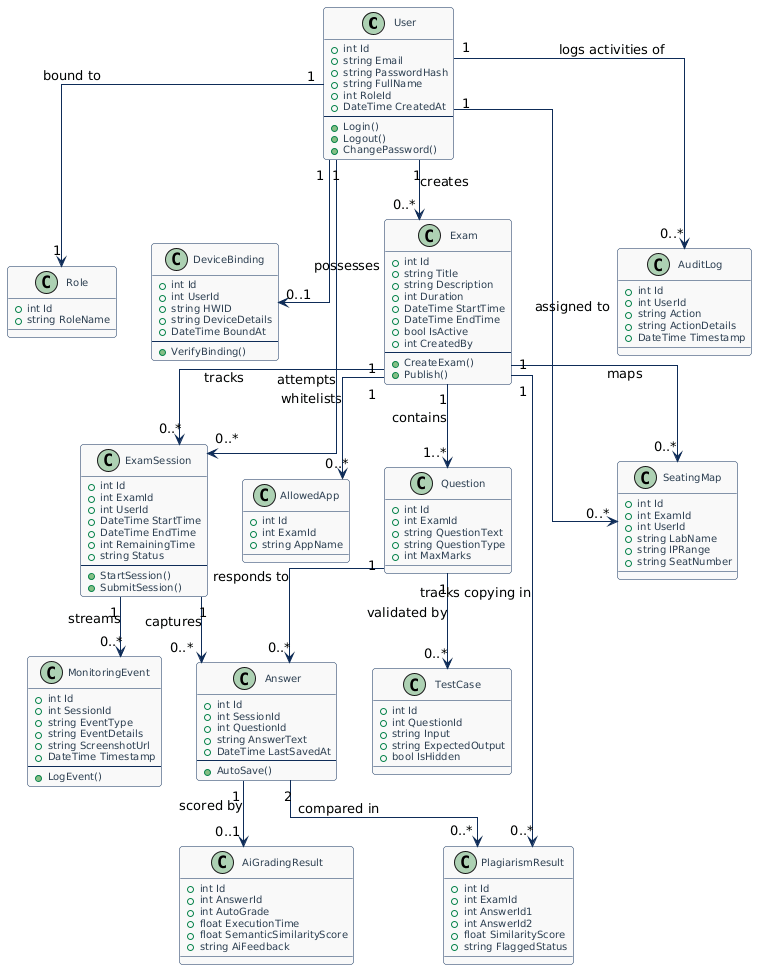
\includegraphics[width=\linewidth,height=628pt,keepaspectratio]{Figures/class_diagram.png}
\caption{Class Diagram of the SmartExam Data Model}
\label{fig:class_diagram}
\end{figure}

\begin{sloppypar}
In the desktop app (Figures~\ref{fig:class_diagram_client} and~\ref{fig:class_diagram_client_b}) the windows hold their view models, and \texttt{LockdownCoordinator} holds the keyboard, process, clipboard, device and Task Manager guards and reports violations to \texttt{LiveMonitoringService}, which owns the webcam monitor with the YuNet \cite{yunet} and YOLOX-Nano \cite{yolox} models. \texttt{ApiClient} is the only class that calls the server.
\end{sloppypar}

\begin{figure}[p]
\centering
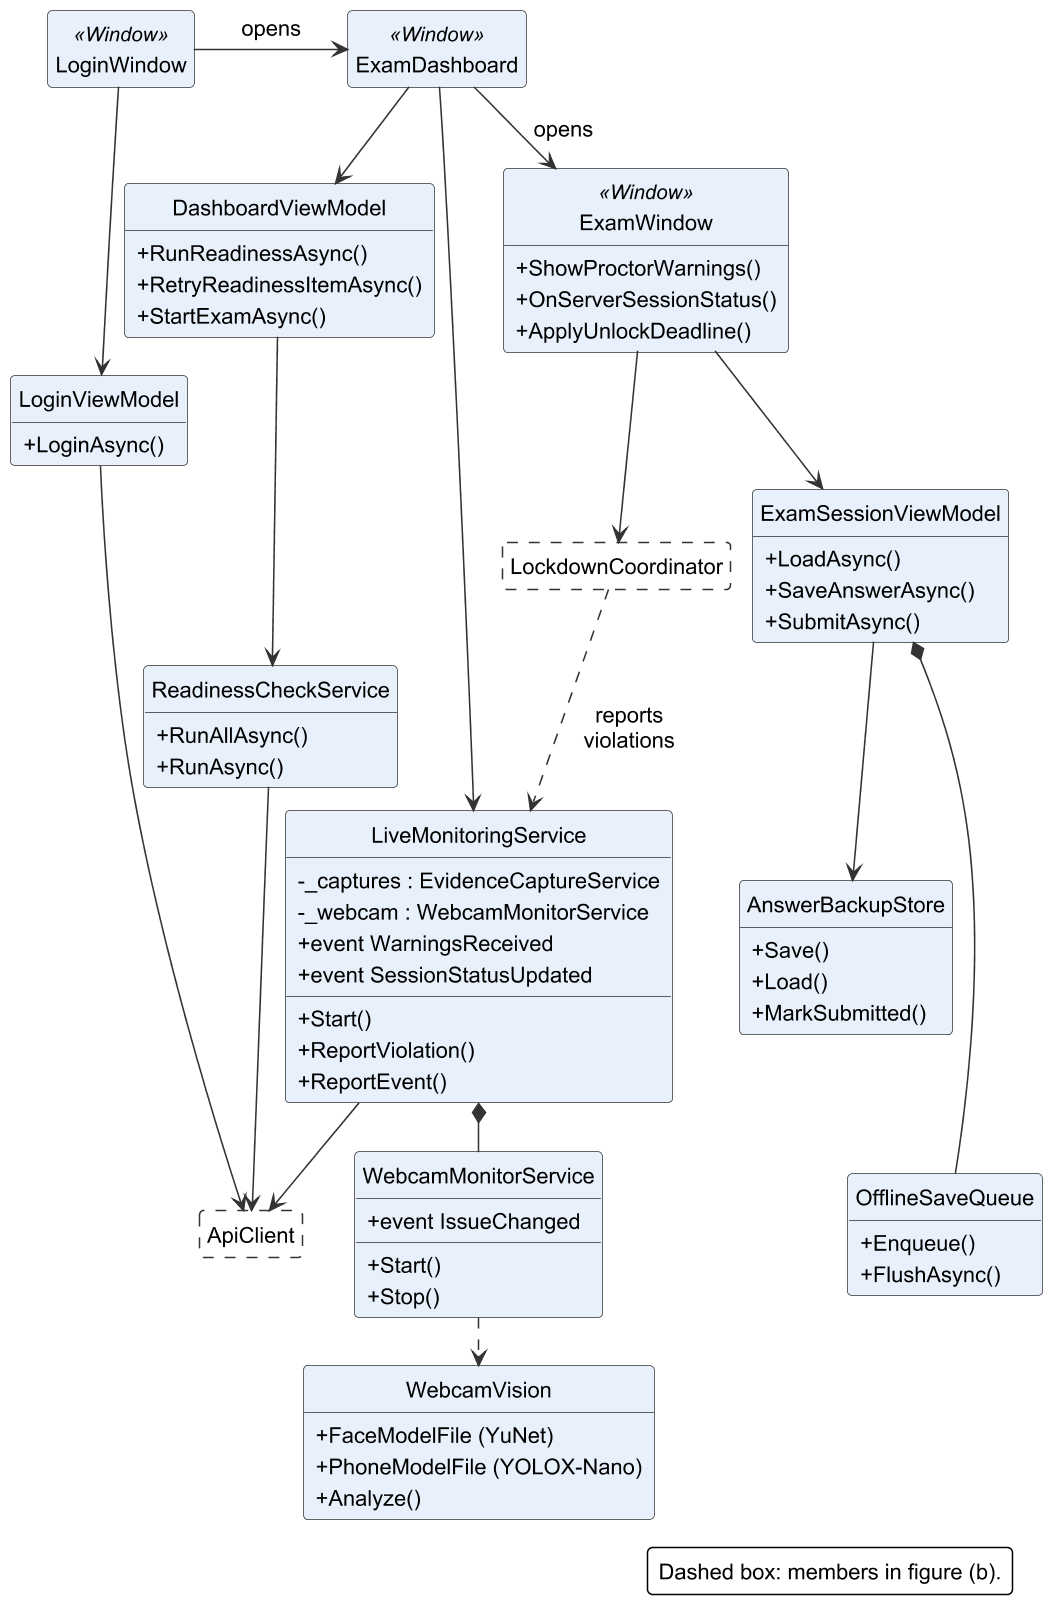
\includegraphics[width=\linewidth,height=590pt,keepaspectratio]{Figures/class_diagram_client.png}
\caption{Class Diagram of the Student Desktop App (a): Windows, View Models, Storage and Monitoring}
\label{fig:class_diagram_client}
\end{figure}

\DiagramBarrier
\begin{figure}[H]
\centering
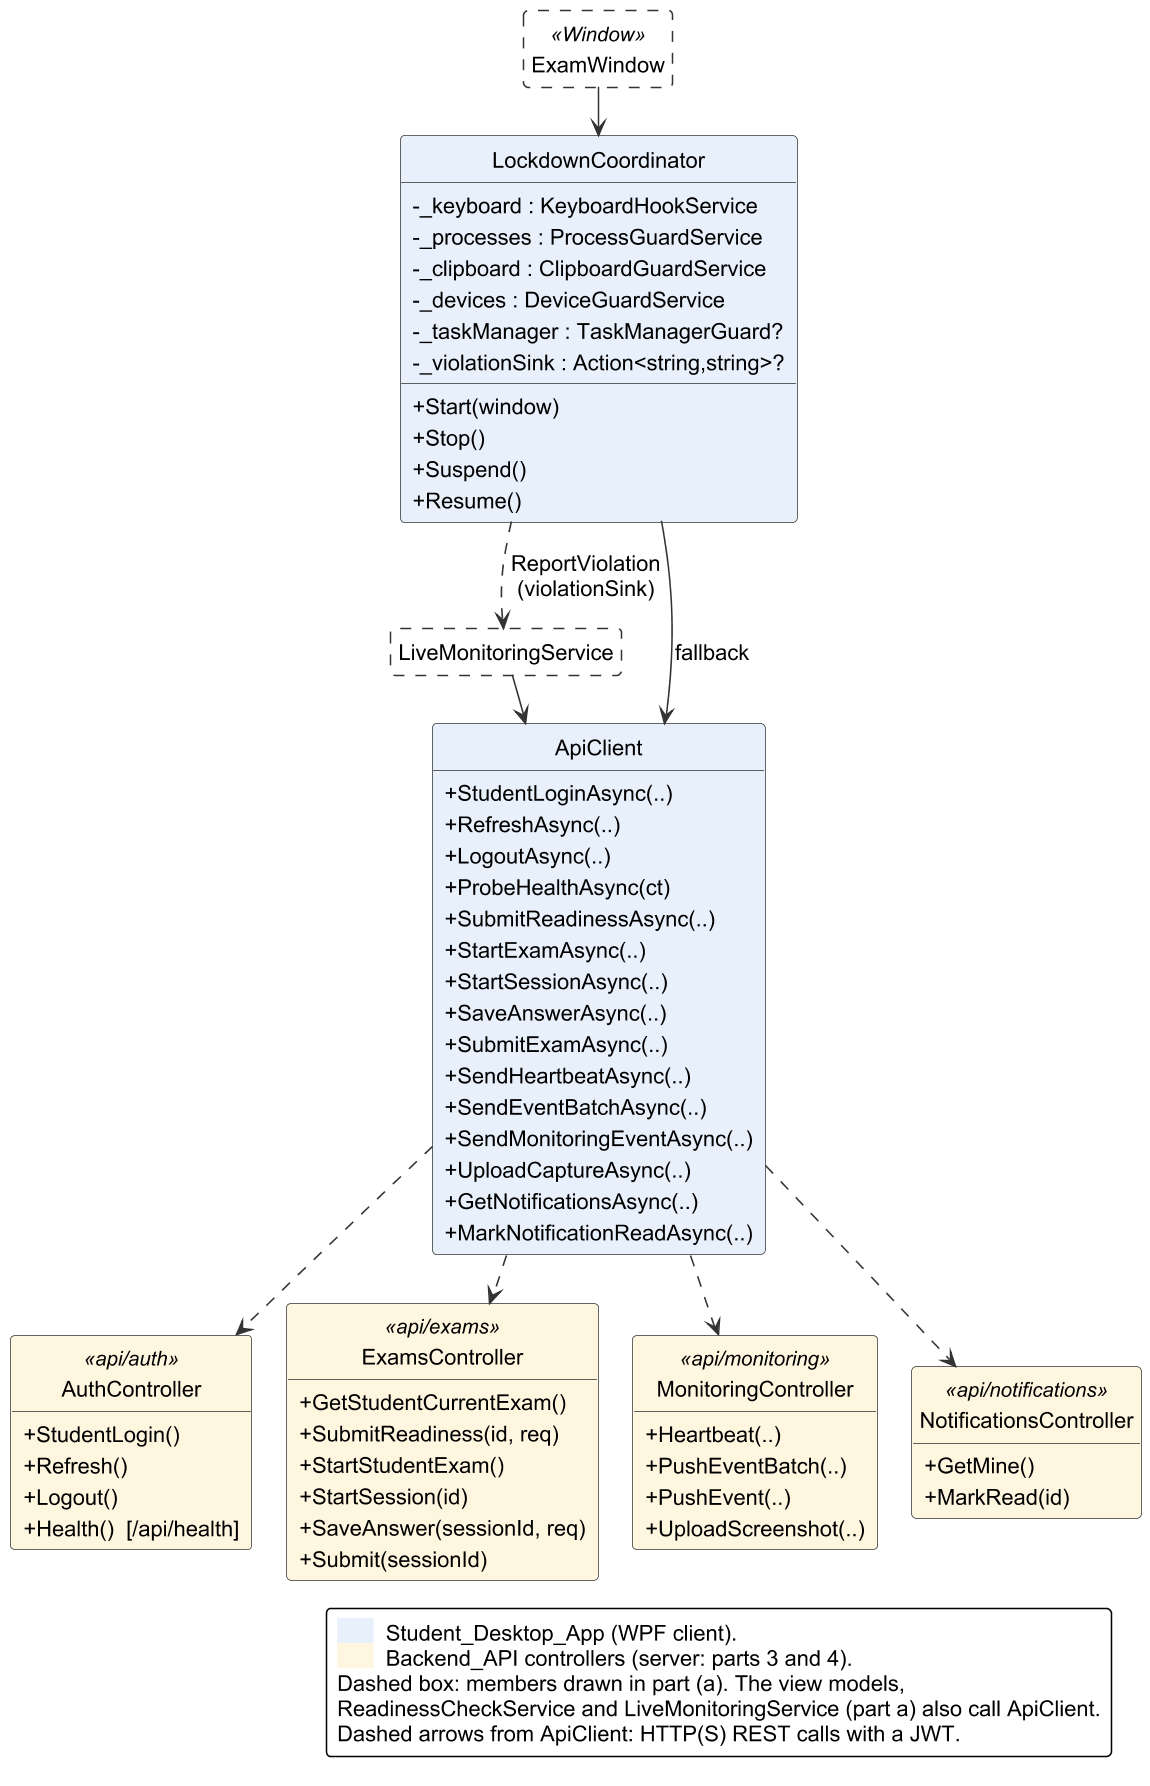
\includegraphics[width=0.95\linewidth,height=628pt,keepaspectratio]{Figures/class_diagram_client_b.png}
\caption{Class Diagram of the Student Desktop App (b): Lockdown, ApiClient and API Controllers}
\label{fig:class_diagram_client_b}
\end{figure}

\begin{sloppypar}
On the server (Figures~\ref{fig:class_diagram_server} and~\ref{fig:class_diagram_server_b}) the controllers and \texttt{MonitoringHub} use \texttt{ExamAccessService}, \texttt{SeatGuard} and \texttt{SubmissionService}; \texttt{GradingWorker} takes queued answers and calls \texttt{GradingService}, which gets a Docker or MinGW \texttt{ICodeRunner} from \texttt{CodeRunnerResolver}. Authentication, evidence, reports and the hash-chained audit trail are in Figures~\ref{fig:class_diagram_server2} and~\ref{fig:class_diagram_server2_b}, where \texttt{AppDbContext} seals new \texttt{AuditLog} rows through \texttt{AuditChain} in \texttt{SaveChanges}.
\end{sloppypar}

\begin{figure}[H]
\centering
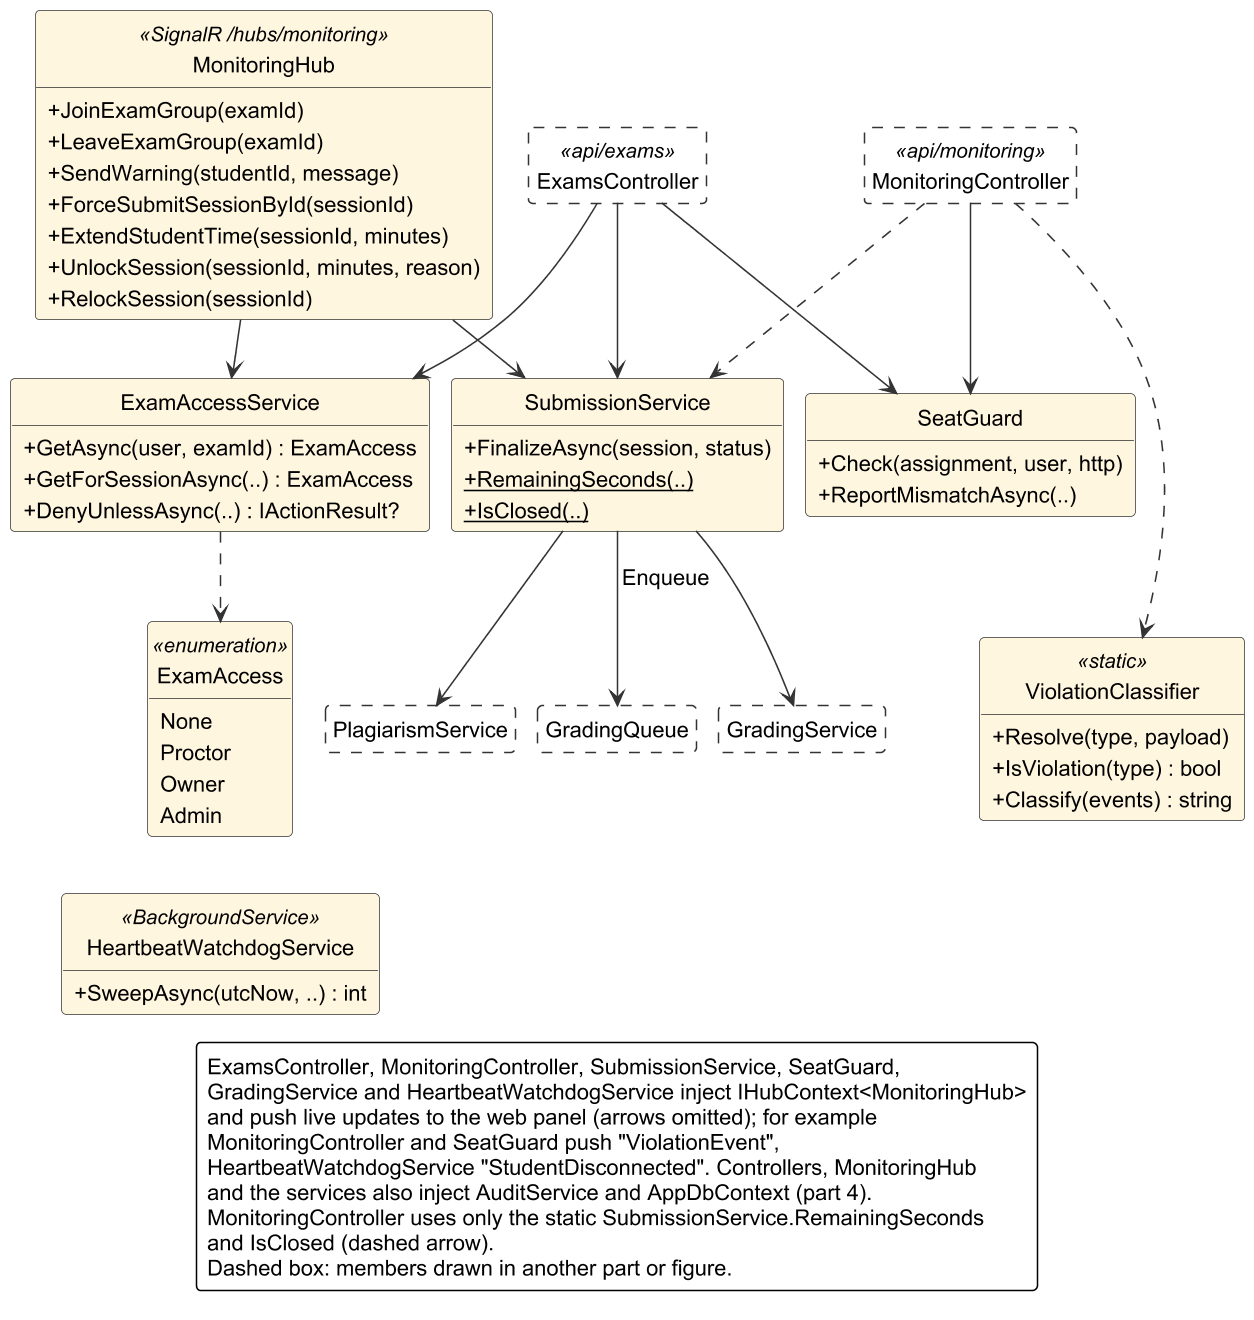
\includegraphics[width=\linewidth,height=469pt,keepaspectratio]{Figures/class_diagram_server.png}
\caption{Class Diagram of the Backend API, Monitoring and Grading (a): Monitoring, Access Checks and Submission}
\label{fig:class_diagram_server}
\end{figure}

\begin{figure}[H]
\centering
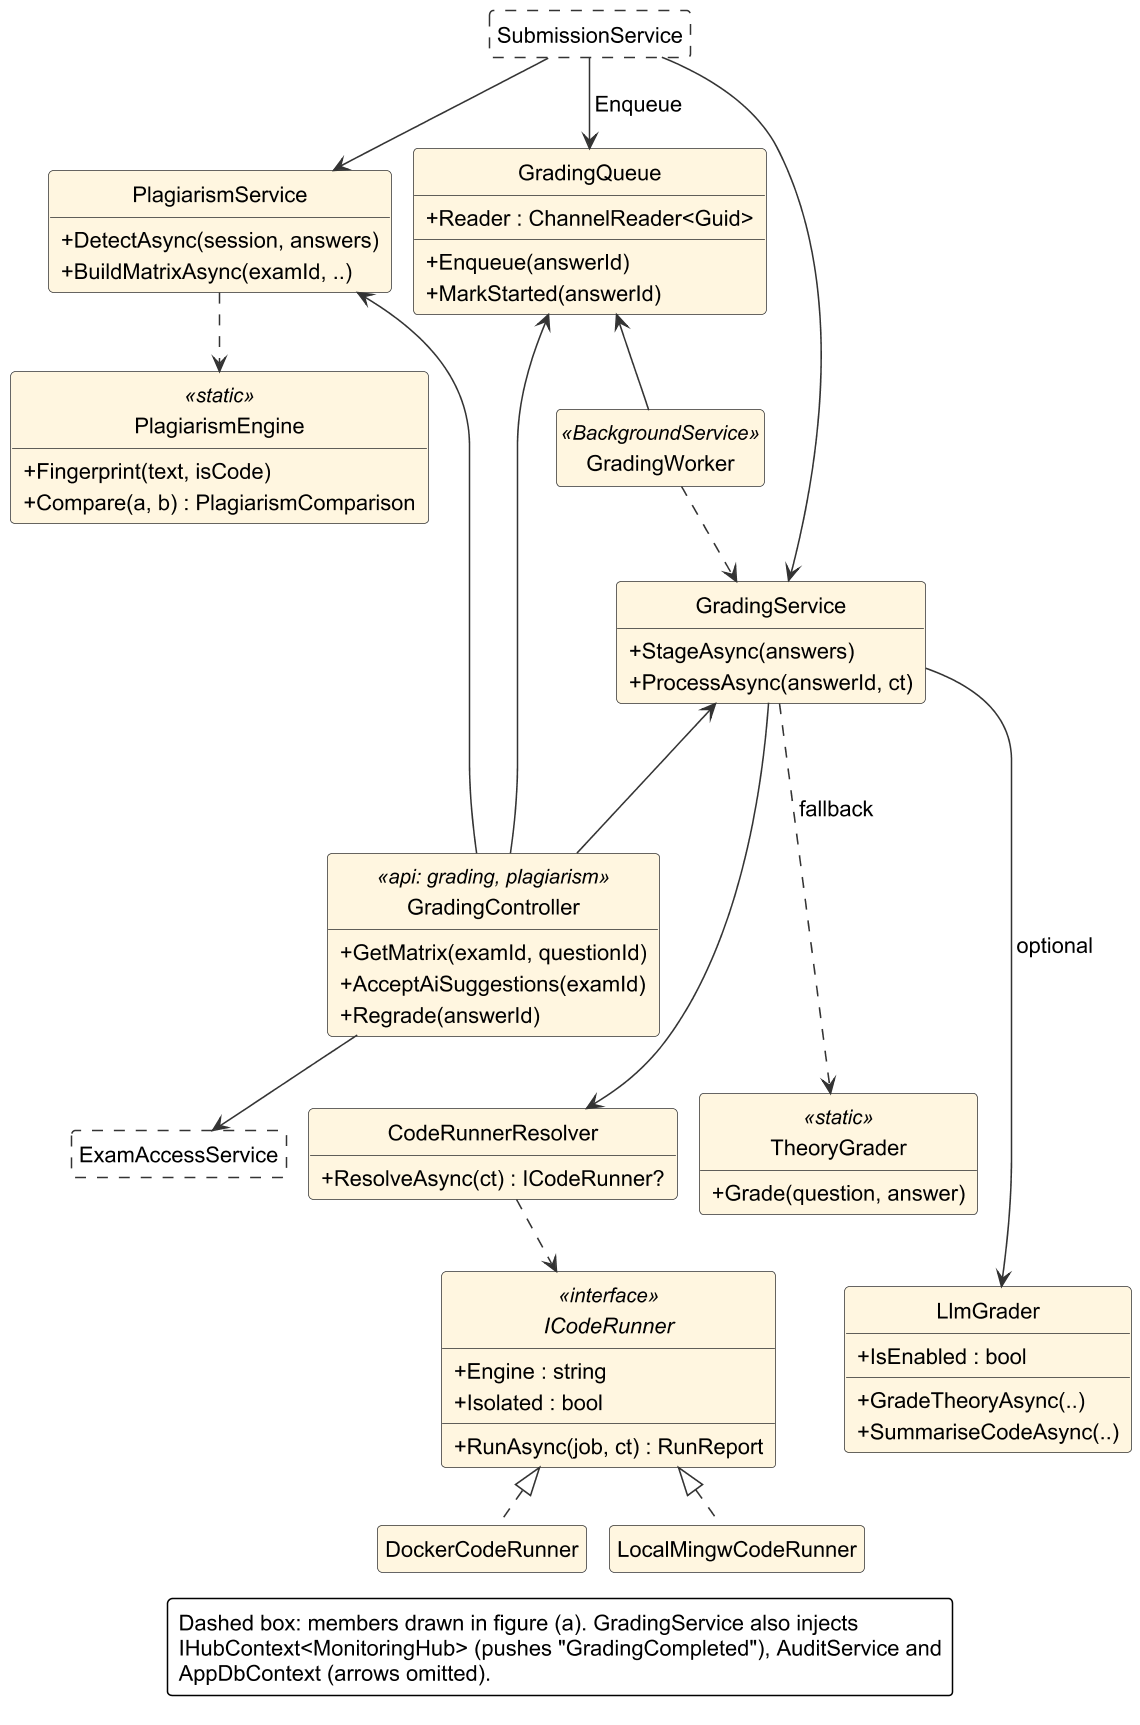
\includegraphics[width=0.95\linewidth,height=628pt,keepaspectratio]{Figures/class_diagram_server_b.png}
\caption{Class Diagram of the Backend API, Monitoring and Grading (b): Grading and Plagiarism}
\label{fig:class_diagram_server_b}
\end{figure}

\begin{figure}[H]
\centering
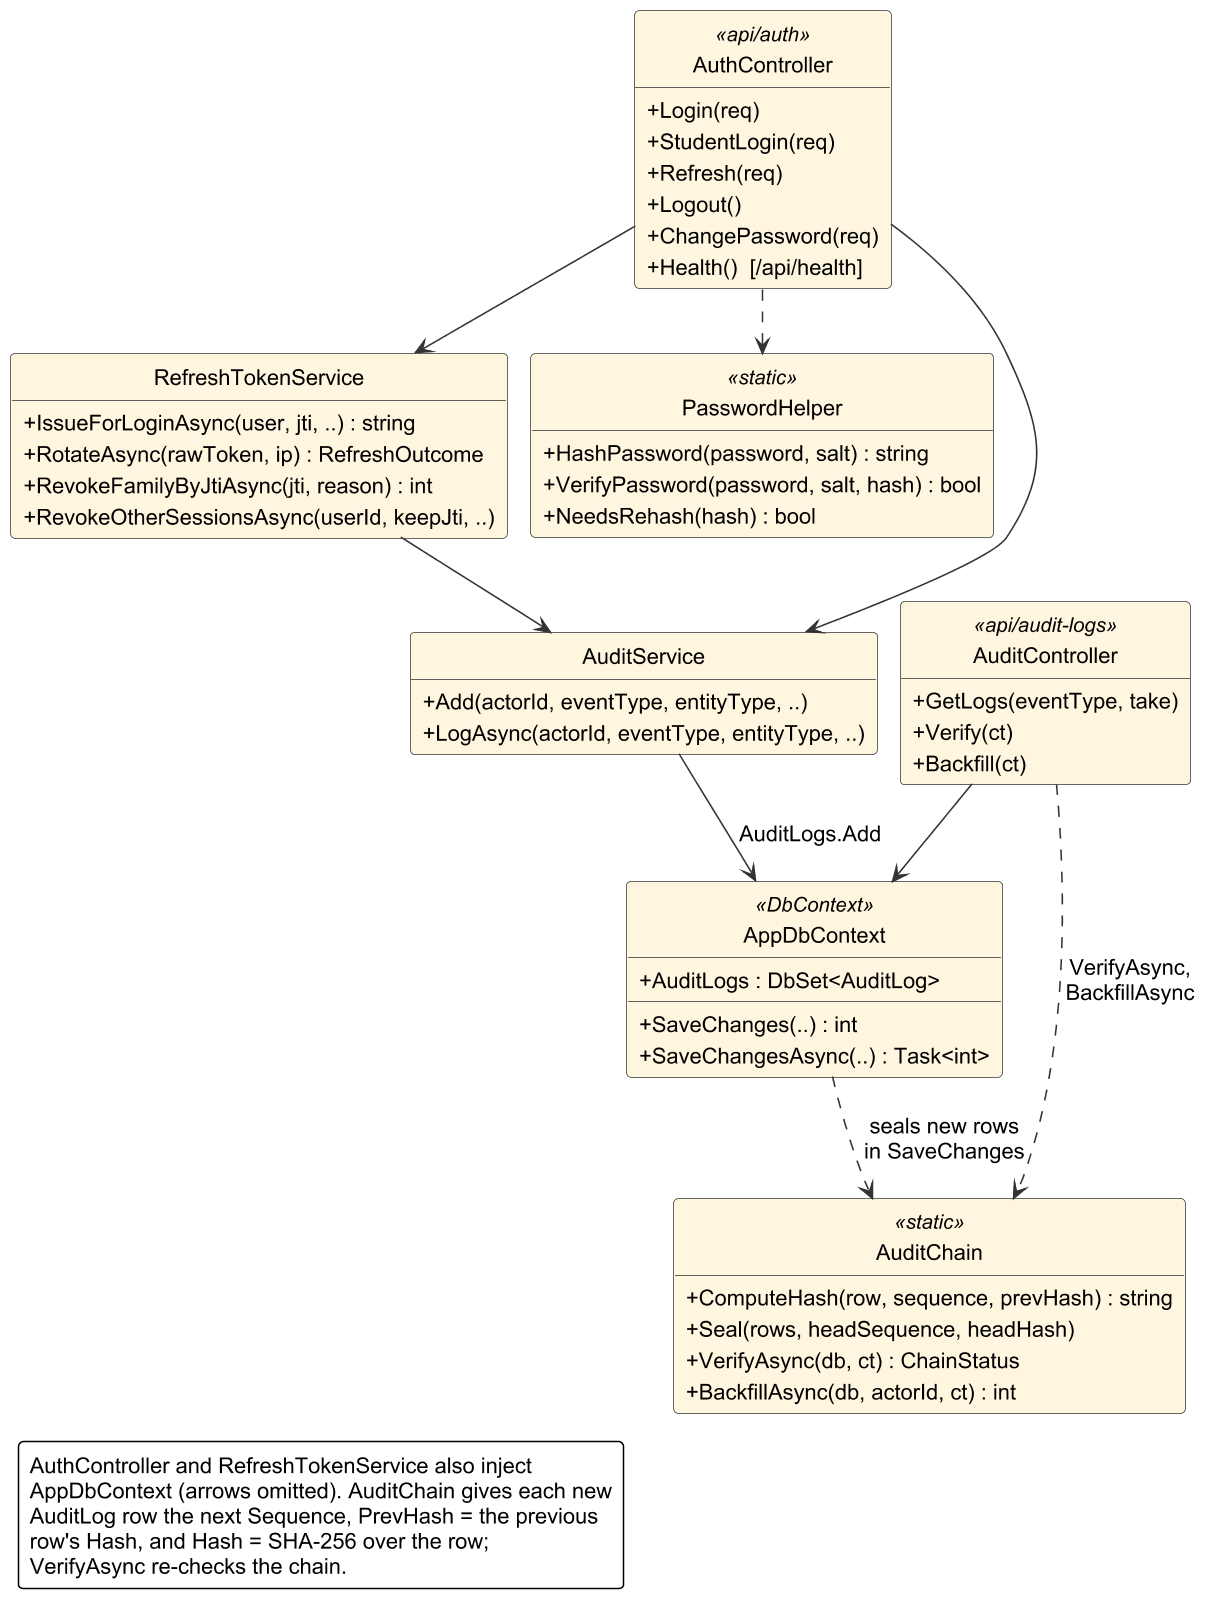
\includegraphics[width=\linewidth,height=604pt,keepaspectratio]{Figures/class_diagram_server2.png}
\caption{Class Diagram of the Backend API, Security and Records (a): Authentication and Audit Trail}
\label{fig:class_diagram_server2}
\end{figure}

\begin{figure}[H]
\centering
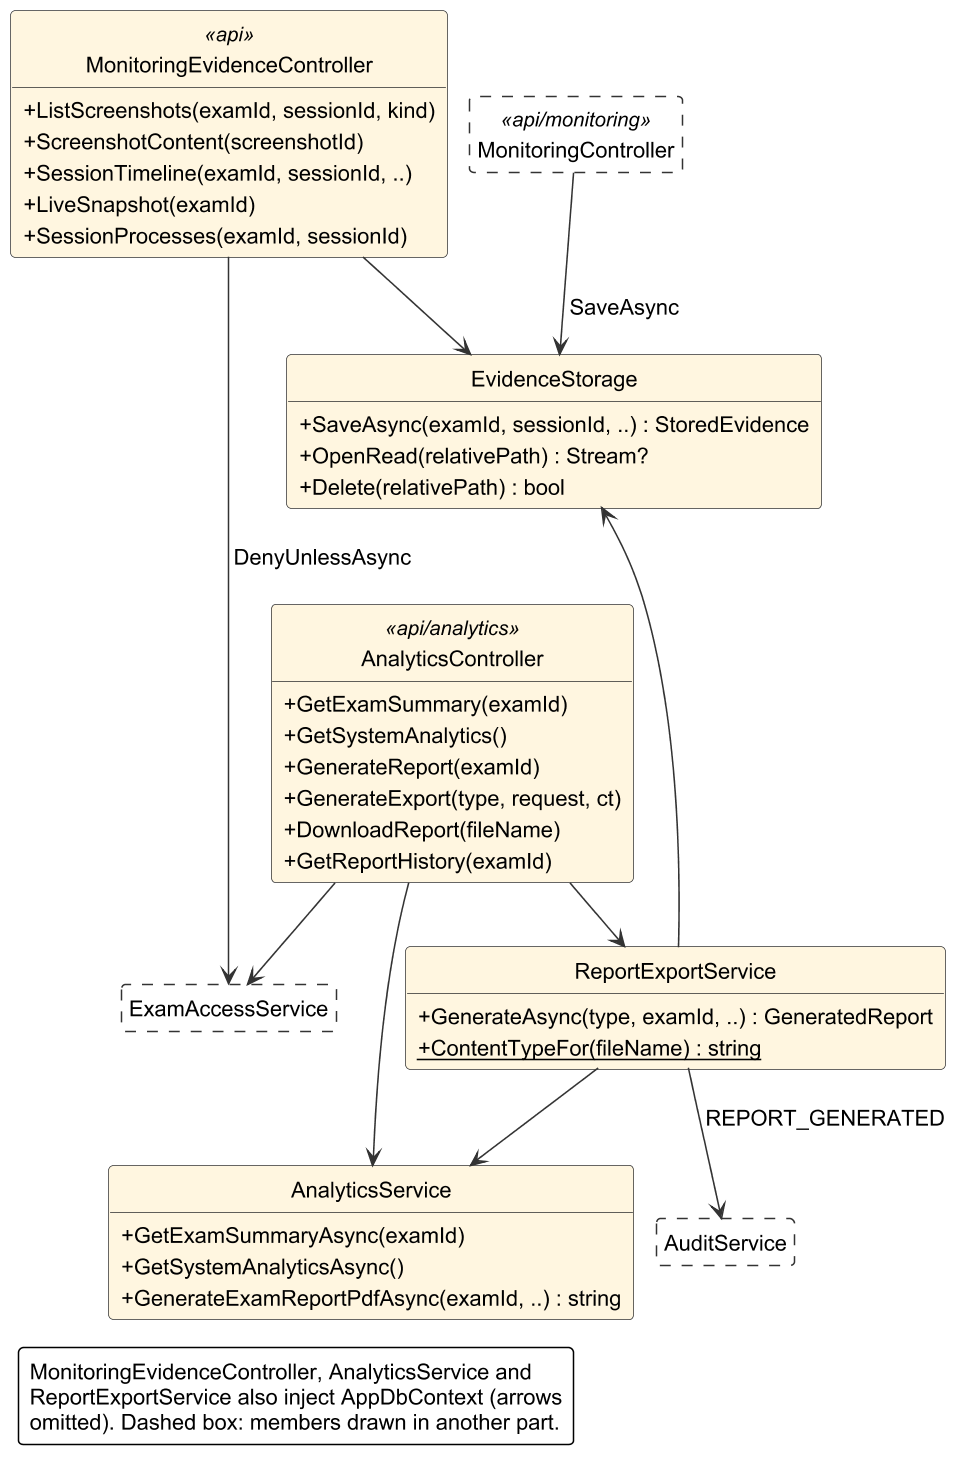
\includegraphics[width=0.80\linewidth,height=556pt,keepaspectratio]{Figures/class_diagram_server2_b.png}
\caption{Class Diagram of the Backend API, Security and Records (b): Evidence and Reports}
\label{fig:class_diagram_server2_b}
\end{figure}

\DiagramBarrier
\subsection{Deployment Diagram}
\begin{sloppypar}
A deployment diagram maps software artefacts onto nodes and communication paths \cite[Cl.~19]{omg_uml251}, \cite{deployment_diagram_vp}. Figure~\ref{fig:deployment_diagram} shows lab workstations running the WPF client with its Open Neural Network Exchange (ONNX) models, encrypted outbox and webcam; browsers running the React panel, whose static build comes from a web host; and an application server whose ASP.NET Core~9 environment runs the API, its SignalR hub (\url{/hubs/monitoring}) and the hosted background services, beside a Docker \texttt{gcc:13} container and a MinGW fallback. The server connects to Neon PostgreSQL, an SMTP server and, optionally, an LLM API. The client and the web panel call the API over REST, using plain HTTP on the shipped localhost configuration and HTTPS behind a Transport Layer Security (TLS) endpoint in a lab deployment; the API itself does not enforce HTTPS. Only the panel adds a SignalR connection, for live updates.
\end{sloppypar}

\begin{figure}[H]
\centering
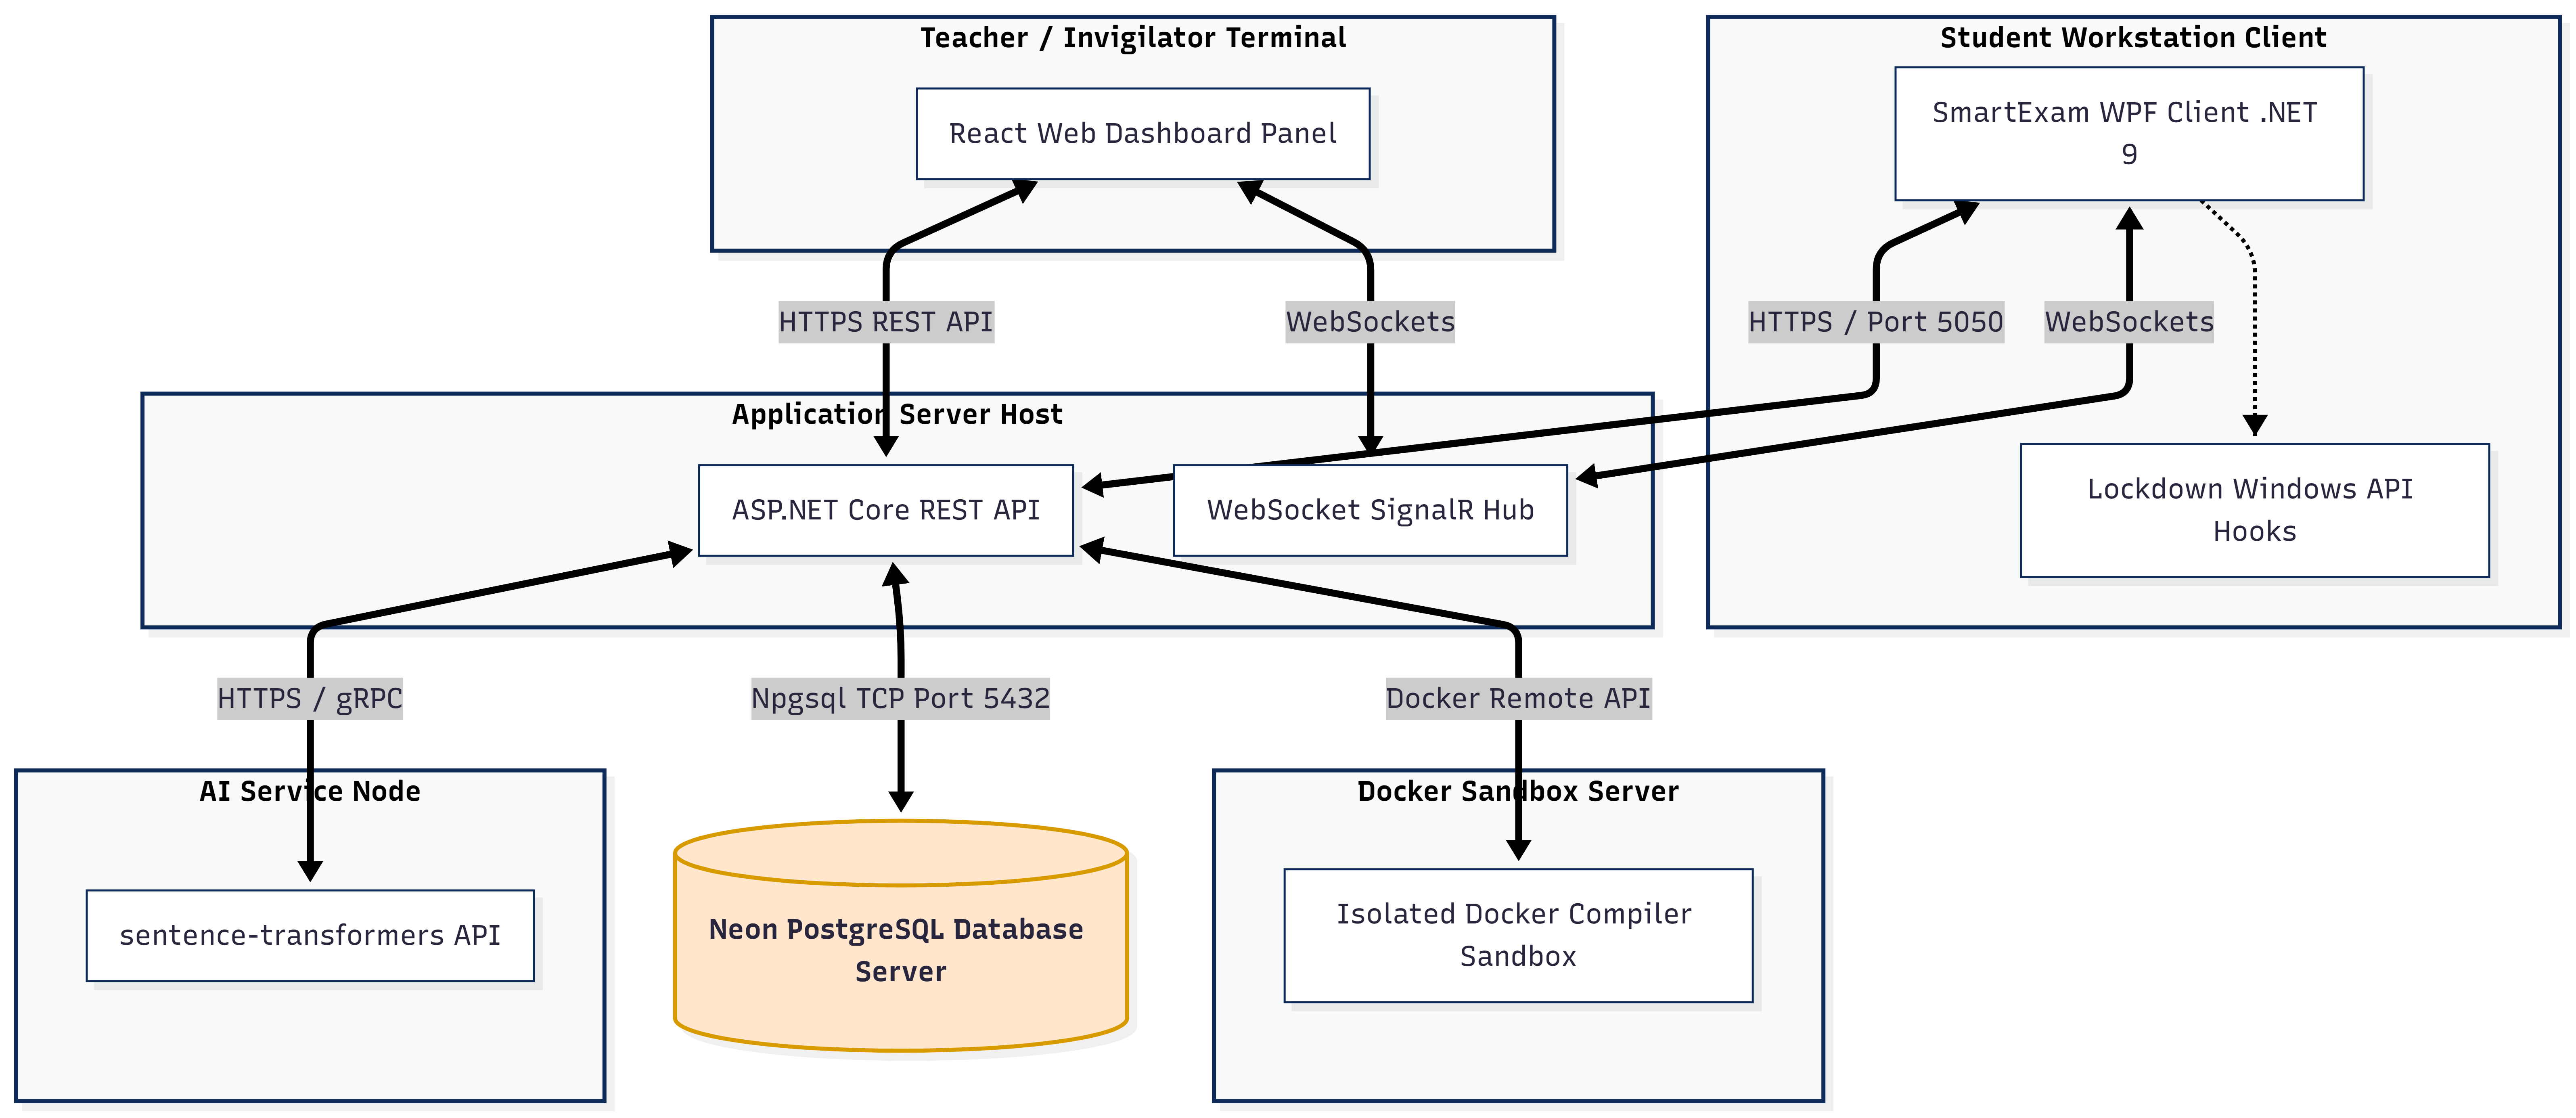
\includegraphics[width=\linewidth,height=360pt,keepaspectratio]{Figures/deployment_diagram.png}
\caption{Deployment Diagram of SmartExam}
\label{fig:deployment_diagram}
\end{figure}

\DiagramBarrier
\subsection{Component Diagram}
\begin{sloppypar}
Figure~\ref{fig:component_diagram} splits the system into client, server and data tiers. The server tier holds the 16 REST controllers, which provide the \url{/api/*} interface (with a JWT), \texttt{MonitoringHub}, which provides \url{/hubs/monitoring}, the domain services (including \texttt{AuditChain} and \texttt{ReportExportService}), hosted services such as \texttt{HeartbeatWatchdogService}, and the grading components. Submission triggers grading and plagiarism detection, and the Grading controller also calls the grading services directly.
\end{sloppypar}

\begin{figure}[p]
\centering
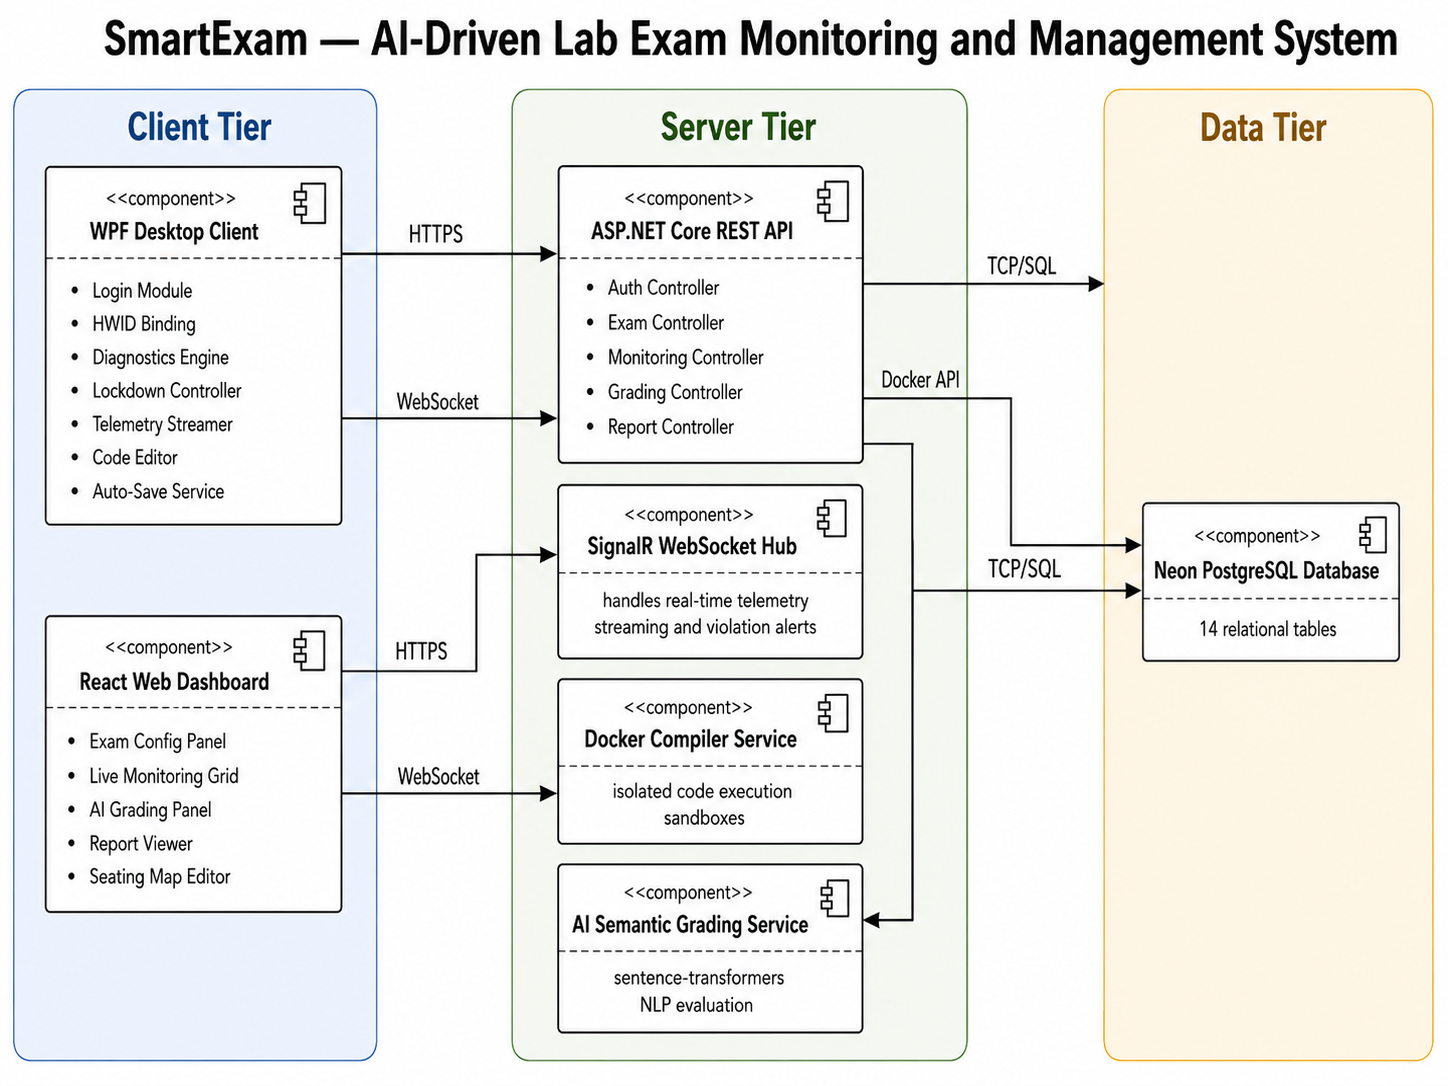
\includegraphics[width=\linewidth,height=628pt,keepaspectratio]{Figures/component_diagram.png}
\caption{Component Diagram of SmartExam}
\label{fig:component_diagram}
\end{figure}

\DiagramBarrier
\section{Behavioural Diagrams}
\label{sec:behavioural_diagrams}
Behavioural diagrams show run-time behaviour: steps, messages and state changes \cite[Annex~A]{omg_uml251}.

\DiagramBarrier
\subsection{Activity Diagrams}
An activity diagram shows a workflow with its decisions and parallel branches \cite[Cl.~15]{omg_uml251}, \cite{activity_diagram_vp}. Figure~\ref{fig:activity_diagram} gives the whole student flow in Student, Desktop App, Server and Teacher swimlanes: login with the device check, readiness checks, the start gate, answering with lockdown and monitoring in parallel, then the end of the session by submit, timer, force-submit or timeout, followed by grading and teacher review.

\begin{figure}[p]
\centering
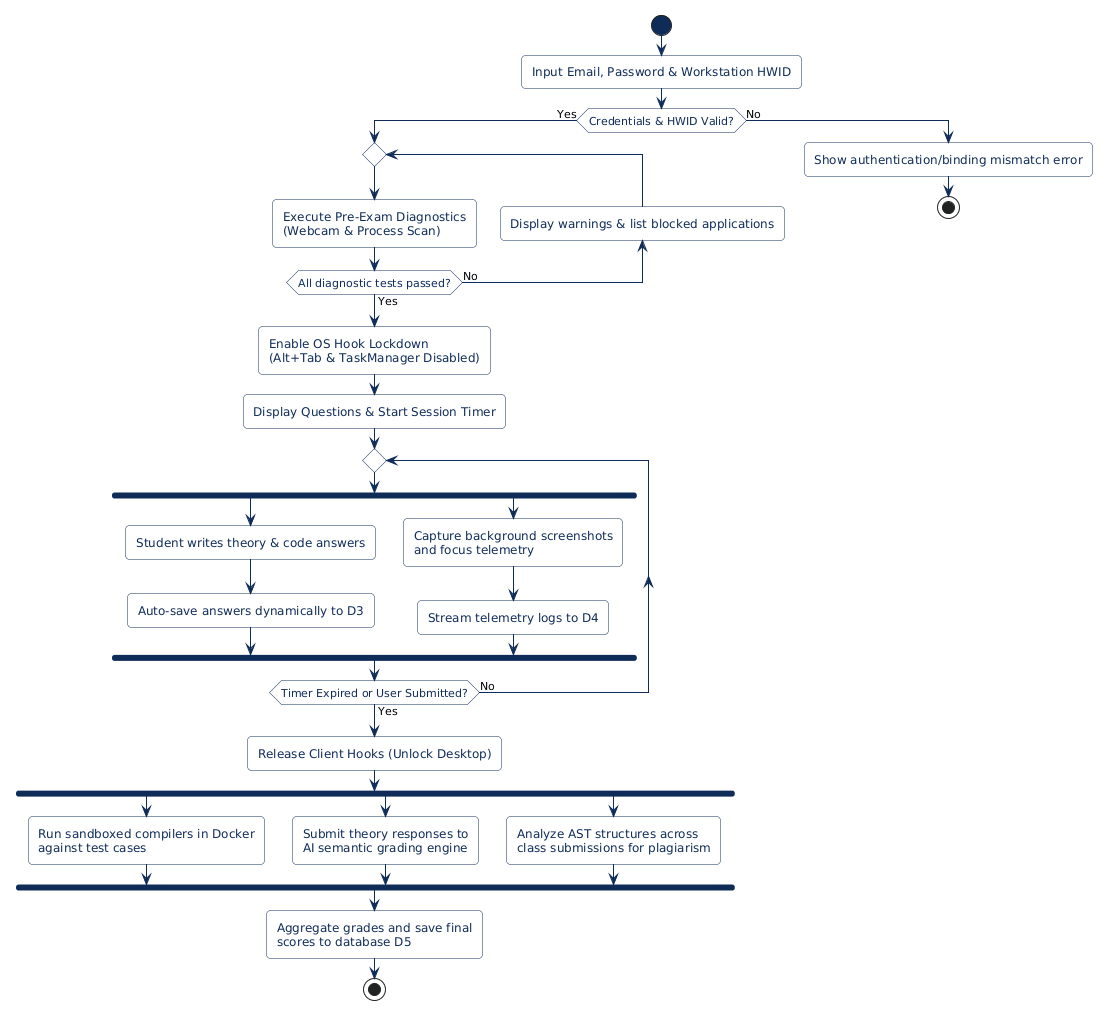
\includegraphics[width=\linewidth,height=618pt,keepaspectratio]{Figures/activity_diagram.png}
\caption{Activity Diagram of the Student Exam Session}
\label{fig:activity_diagram}
\end{figure}

\subsubsection{Login and Pre-Exam Checks (M1, M2; UC-01, UC-02)}
\begin{sloppypar}
In Figure~\ref{fig:activity_auth} the client sends the email or roll number, the password and a hardware fingerprint to \url{/api/auth/student-login}, which accepts 10 requests a minute per IP address and then returns 429. The v2 fingerprint joins the BIOS, system-disk and baseboard serials read through WMI; the server stores only its SHA-256 hash. Wrong credentials return 401 (\texttt{LOGIN\_FAILED}); a non-student account or a missing HWID is refused without an audit entry. The first login saves the hash as the student's \texttt{DeviceBinding} (\texttt{DEVICE\_BOUND}), an old v1 binding is upgraded when the legacy fingerprint matches (\texttt{DEVICE\_REBOUND}), and a login from another machine is refused with \texttt{DEVICE\_MISMATCH}. A successful login re-hashes a password stored with an older scheme, is audited as \texttt{LOGIN\_SUCCESS} and returns a JWT and a refresh token.
\end{sloppypar}

\begin{figure}[p]
\centering
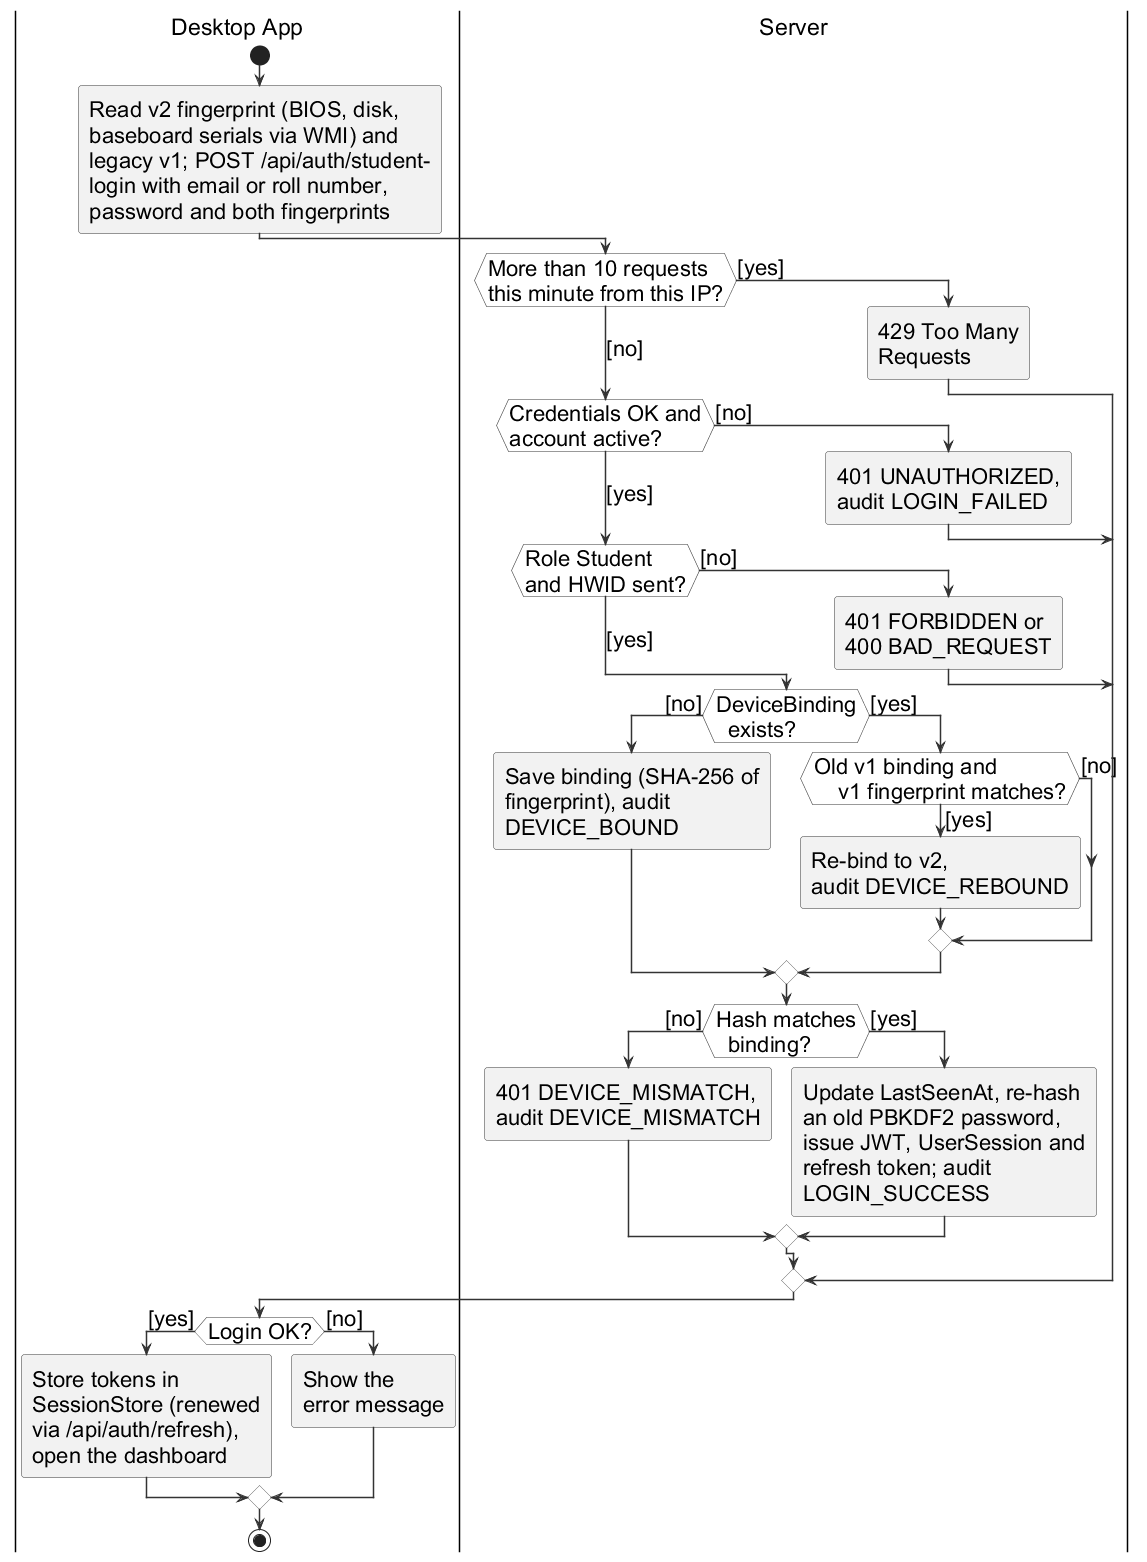
\includegraphics[width=\linewidth,height=615pt,keepaspectratio]{Figures/activity_auth.png}
\caption{Activity Diagram of Student Login and HWID Binding}
\label{fig:activity_auth}
\end{figure}

Figure~\ref{fig:activity_diagnostics} shows the seven checks in \texttt{ReadinessPolicy}: network, clock skew, screen capture, webcam (one face, by YuNet) and microphone (when required), secure mode and disk space. Every run or retry posts all results to \url{/api/exams/{id}/readiness}, where the server recomputes the pass, audits it as \texttt{READINESS\_PASSED} or \texttt{READINESS\_FAILED} and pushes \texttt{ReadinessUpdated}. A pass is valid for 30 minutes, and Start unlocks once the exam opens.

\DiagramBarrier
\begin{figure}[H]
\centering
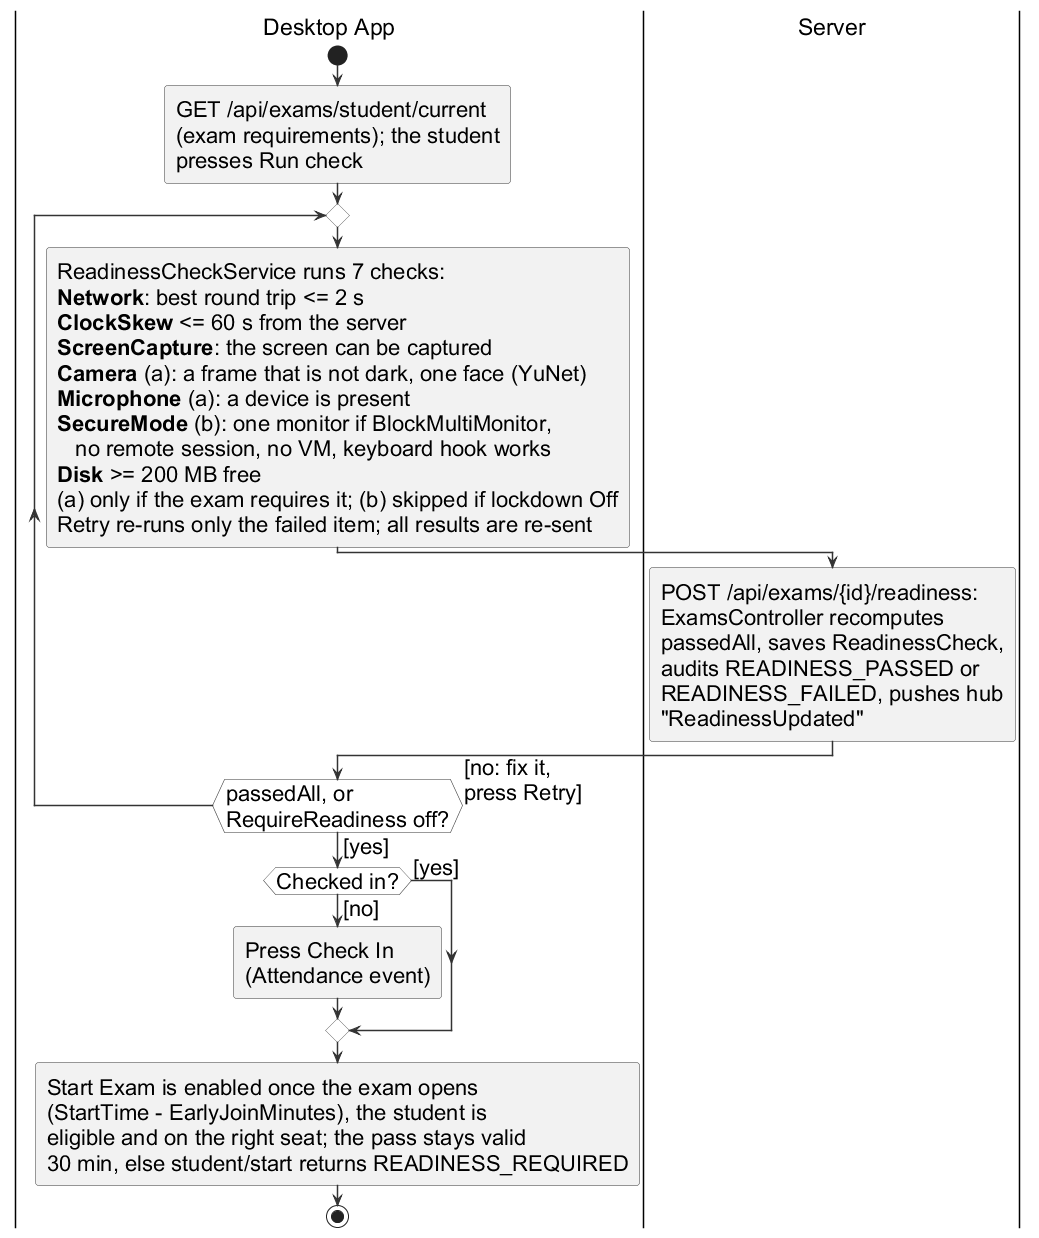
\includegraphics[width=0.85\linewidth,height=457pt,keepaspectratio]{Figures/activity_diagnostics.png}
\caption{Activity Diagram of Pre-Exam Readiness Checks}
\label{fig:activity_diagnostics}
\end{figure}

\DiagramBarrier
\subsubsection{Practice Exam and Exam Workspace (M2, M4, M5; UC-03, UC-06, UC-07)}
\begin{sloppypar}
Practice exams (\texttt{Exam.IsMock}) are picked from the dashboard's practice list and started with \texttt{POST} \url{/api/exams/{id}/start-session} instead of the real exam's \url{/api/exams/student/start}. They run in the same exam window, in Report mode and without the webcam, so students meet the editor and lockdown beforehand (Figure~\ref{fig:activity_readiness}). Practice exams do not count towards results: they are auto-marked when AI evaluation is on, but never checked for plagiarism and left out of the student's results and analytics.
\end{sloppypar}

\begin{figure}[H]
\centering
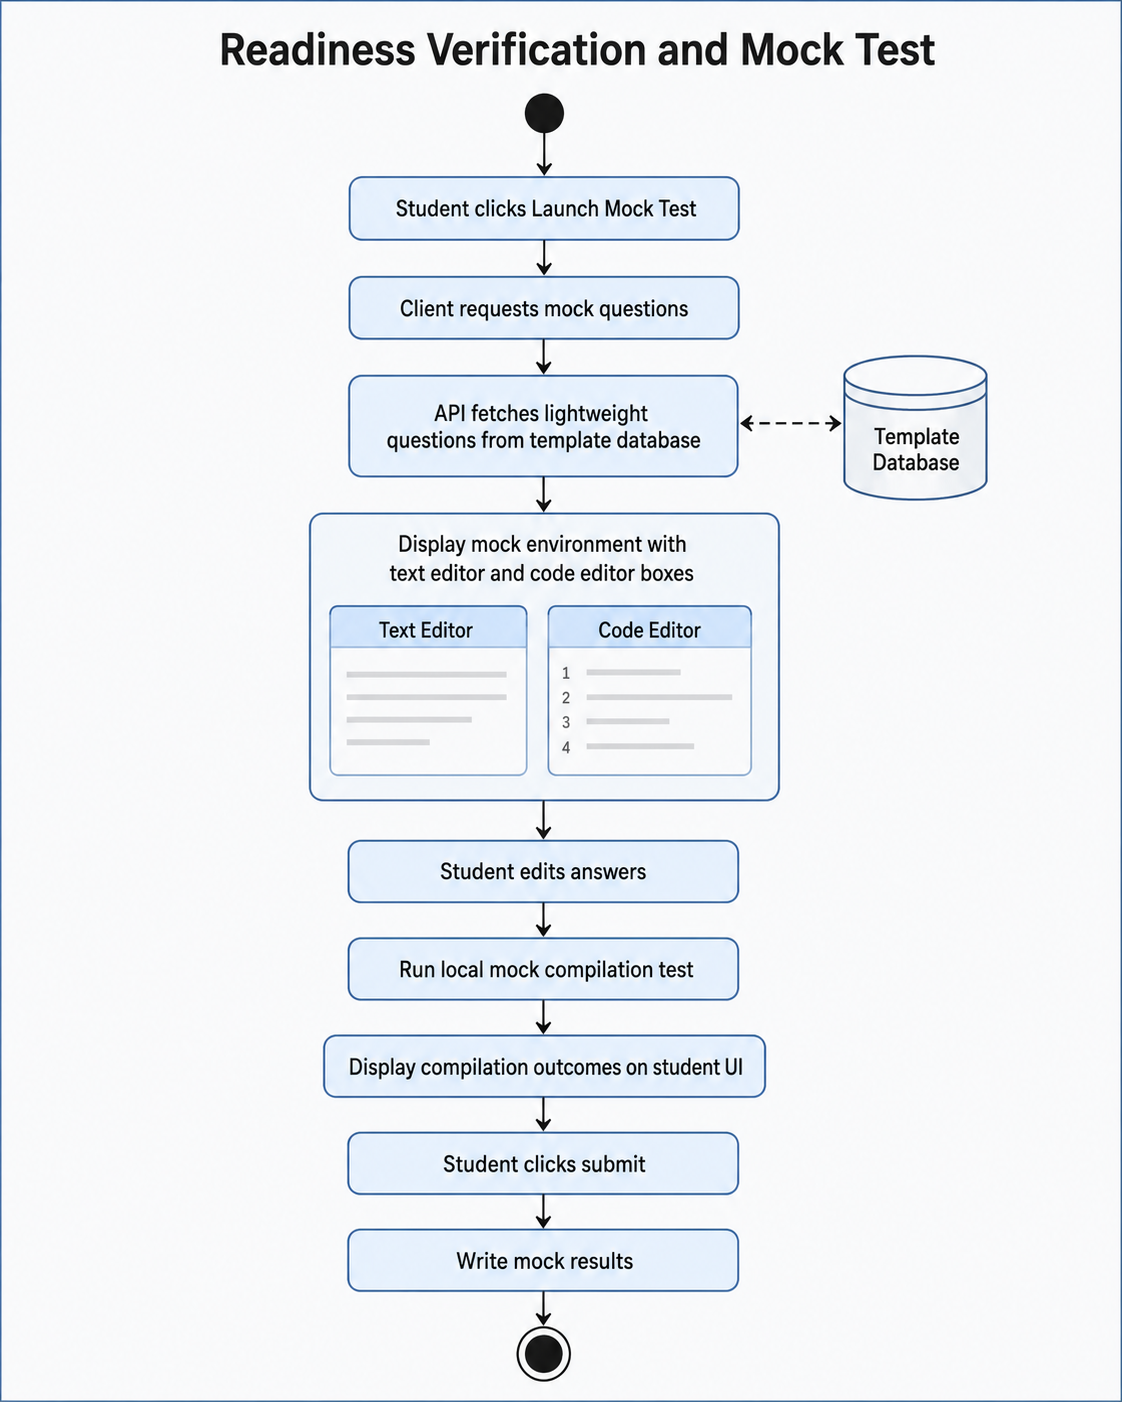
\includegraphics[width=0.80\linewidth,height=366pt,keepaspectratio]{Figures/activity_readiness.png}
\caption{Activity Diagram of the Practice Exam}
\label{fig:activity_readiness}
\end{figure}

\begin{sloppypar}
During an exam (Figure~\ref{fig:activity_dashboard}) the window runs fullscreen under \texttt{LockdownCoordinator} and, when required, the webcam monitor. Four regions run concurrently. The student answers questions. A heartbeat goes out every 10 seconds, and its ack brings the remaining time, session status, extra time, up to five warnings and the unlock deadline. Guard events (a blocked key, clipboard use, a disallowed app, a focus loss, USB storage or a webcam issue) go to \url{/api/monitoring/events/batch}, while a rate-limited screen capture, plus a webcam snapshot for a webcam issue, is uploaded separately to \url{/api/monitoring/screenshot}. The server stores each item and pushes it to the live monitor.
\end{sloppypar}

\begin{figure}[H]
\centering
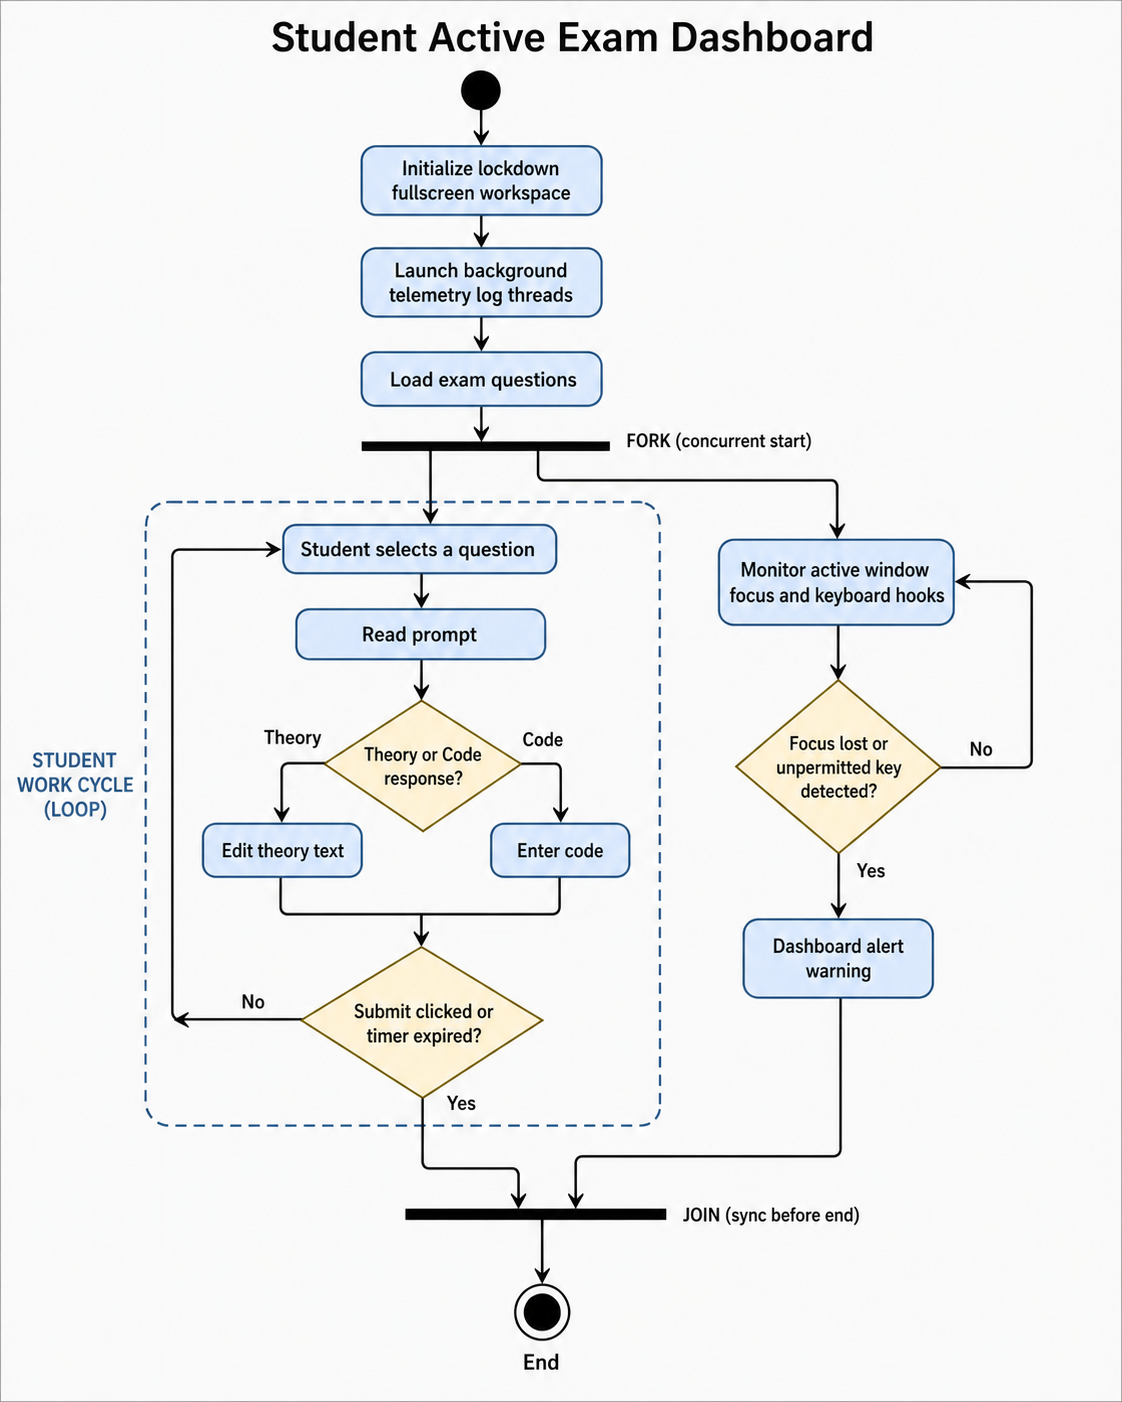
\includegraphics[width=\linewidth,height=395pt,keepaspectratio]{Figures/activity_dashboard.png}
\caption{Activity Diagram of the Active Exam Workspace}
\label{fig:activity_dashboard}
\end{figure}

\DiagramBarrier
\subsubsection{Autosave, Recovery and Submission (M6; UC-08)}
An answer is saved 10 seconds after its first unsaved edit, on question change and on focus loss. Within a second, every edit also goes to a local backup encrypted with AES-256 in Galois/Counter Mode (AES-256-GCM) \cite{nist80038d}, whose key is protected by the Windows Data Protection API (DPAPI). Failed saves are queued and replayed when the network returns. If a crash or power cut closed the exam, the relaunched client resumes the same session and merges the backup with the server copy, the higher revision winning (Figure~\ref{fig:activity_recovery}).

\begin{figure}[H]
\centering
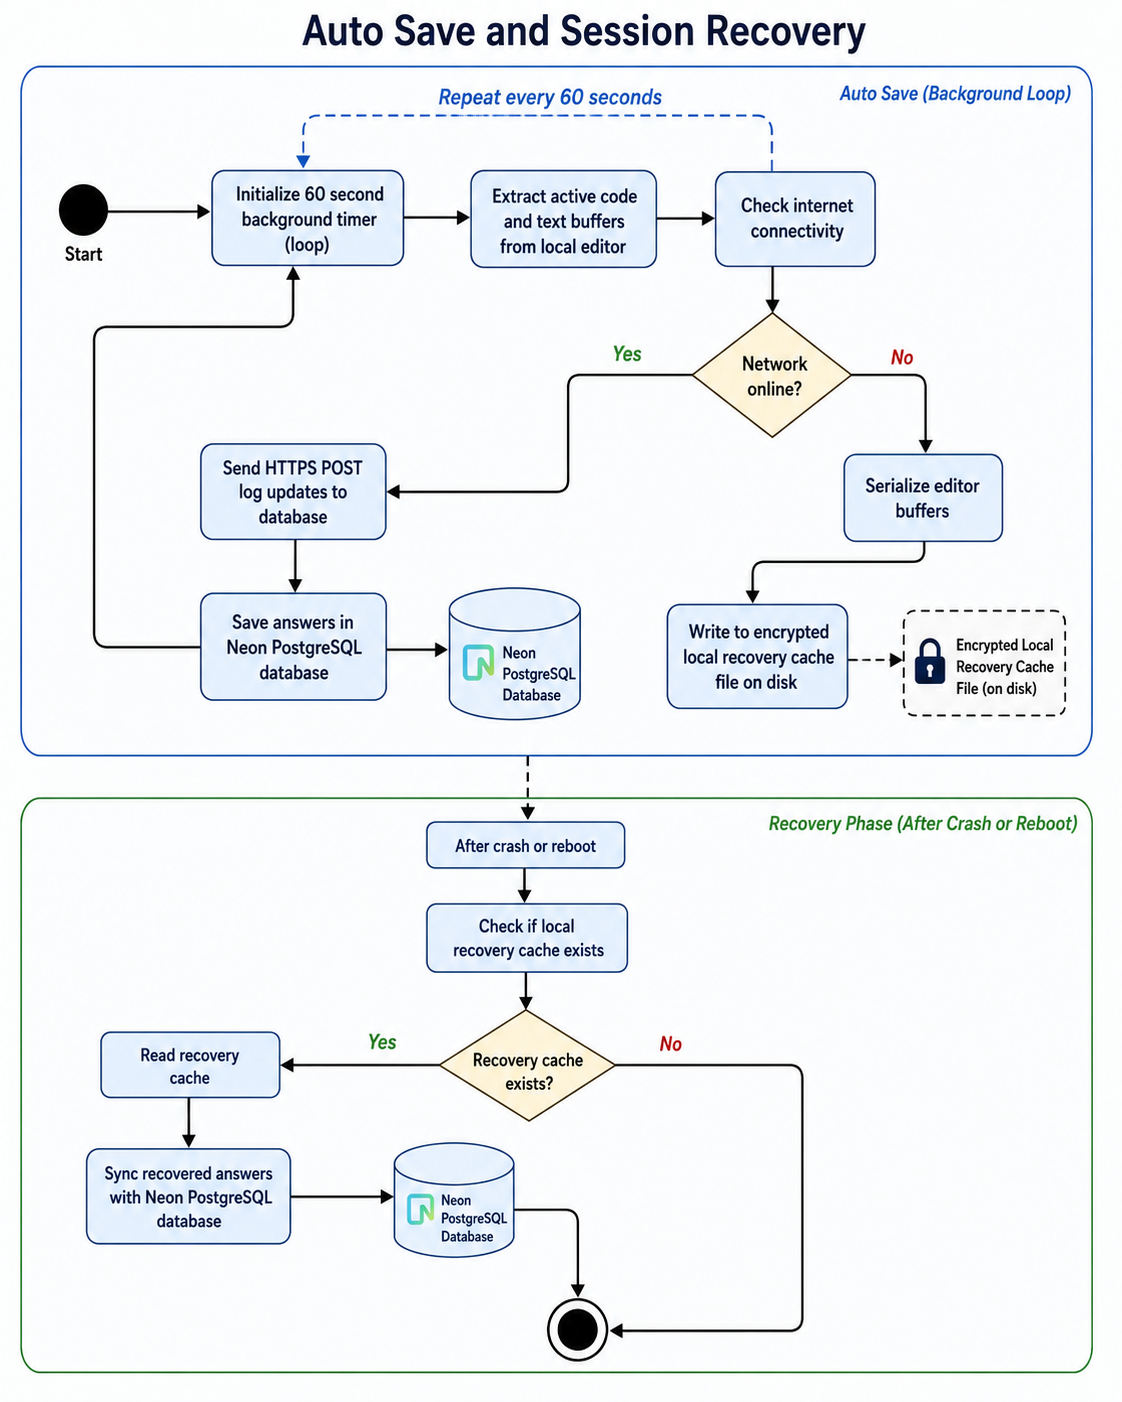
\includegraphics[width=\linewidth,height=498pt,keepaspectratio]{Figures/activity_recovery.png}
\caption{Activity Diagram of Autosave and Session Recovery}
\label{fig:activity_recovery}
\end{figure}

Submission starts when the timer reaches zero or when the student confirms the dialog that counts unanswered questions (Figure~\ref{fig:activity_submission}). The client flushes pending saves; if an answer is still unsent it keeps the window open: an automatic submit retries every 10 seconds, and after a manual submit the student presses Submit again. Otherwise it submits, and \texttt{FinalizeAsync} sets the session to Submitted with a SHA-256 receipt, which the client verifies. If no submit arrives, \texttt{SessionTimeoutService} sweeps every 30 seconds and finalises sessions past the exam end, extra time and a 2-minute grace as TimedOut.

\begin{figure}[p]
\centering
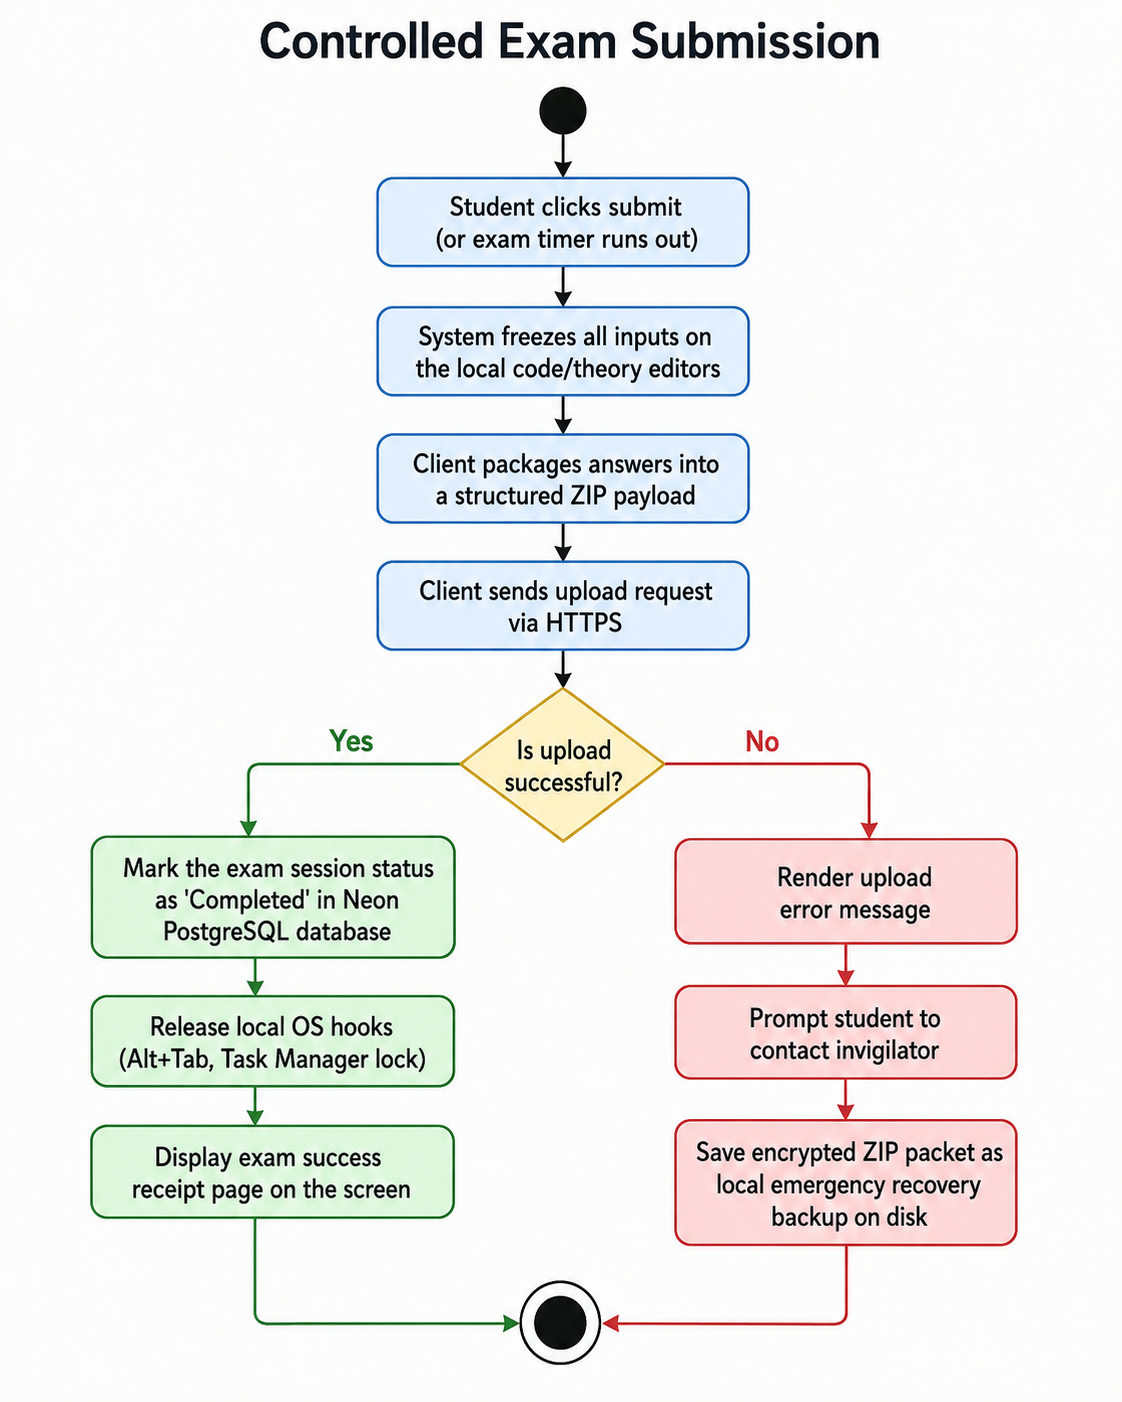
\includegraphics[width=\linewidth,height=628pt,keepaspectratio]{Figures/activity_submission.png}
\caption{Activity Diagram of Exam Submission}
\label{fig:activity_submission}
\end{figure}

\DiagramBarrier
\subsubsection{Exam Configuration (M4, M8; UC-06, UC-13)}
A teacher fills a four-step wizard (basic info, questions, rules, students) to create or edit an exam (Figure~\ref{fig:activity_config}). \texttt{ExamsController} validates the payload, for example requiring a test case for every coding question, and refuses students outside the teacher's sections; an exam can be edited only while it is Scheduled. The exam is saved together with its \texttt{EXAM\_CREATED} or \texttt{EXAM\_UPDATED} audit entry.

\begin{figure}[p]
\centering
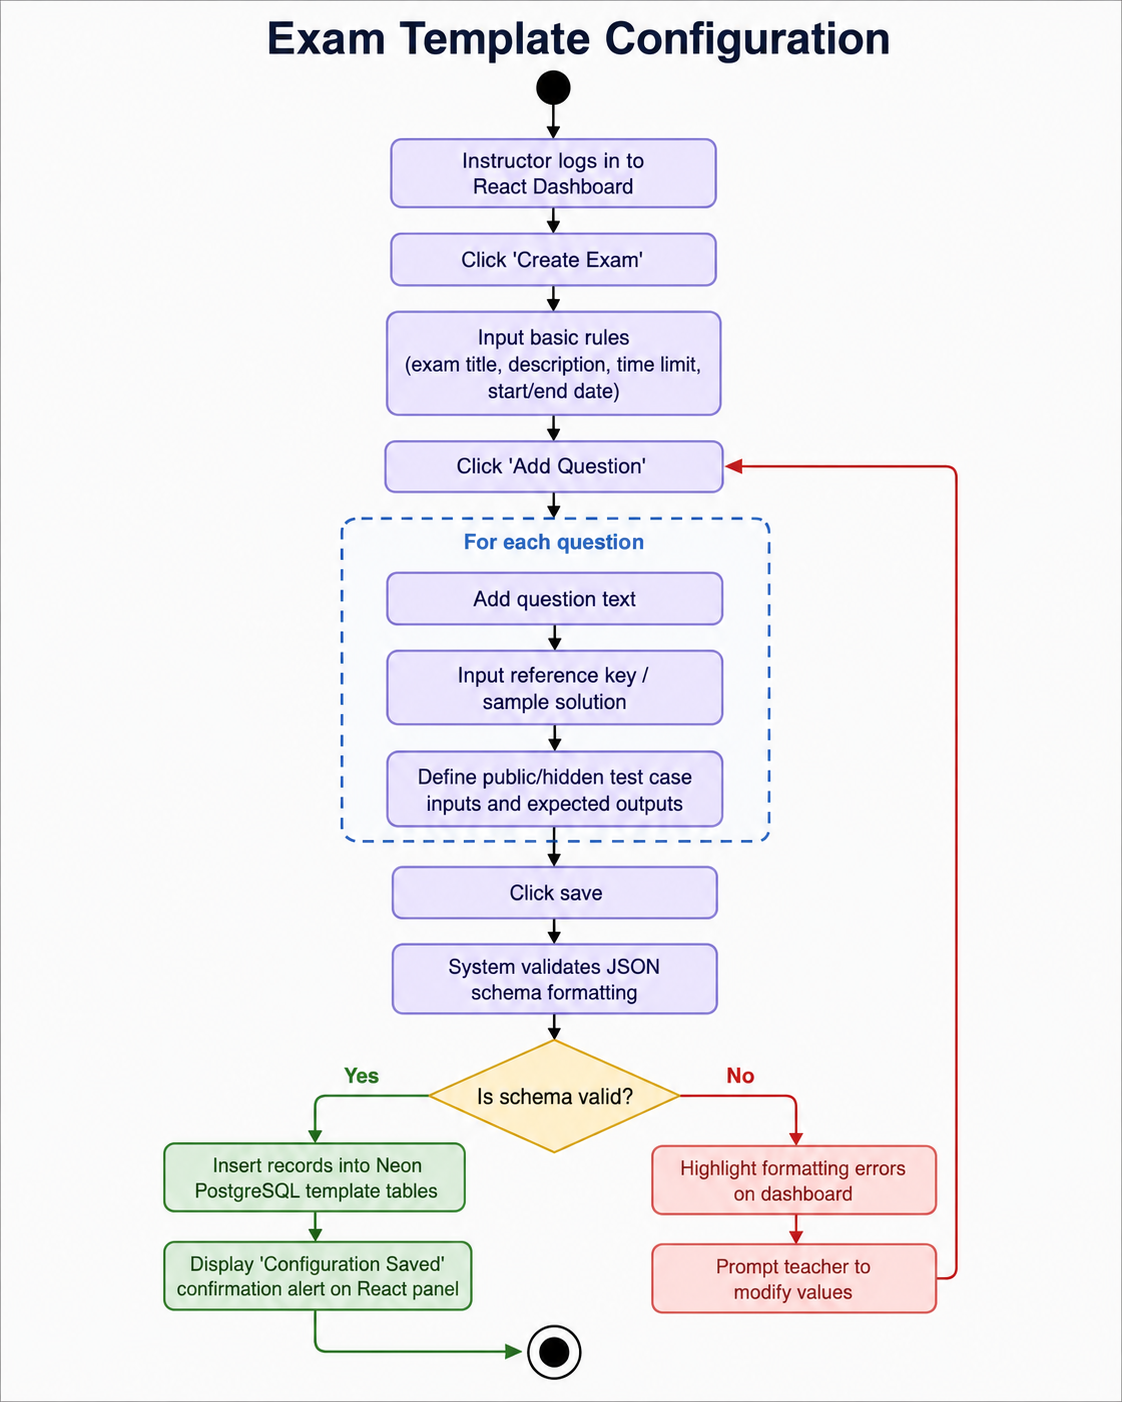
\includegraphics[width=\linewidth,height=528pt,keepaspectratio]{Figures/activity_config.png}
\caption{Activity Diagram of Exam Configuration}
\label{fig:activity_config}
\end{figure}

\begin{sloppypar}
Allowed applications are stored as a JSON list of executable names in \texttt{Exam.AllowedApps} (Figure~\ref{fig:activity_applications}). \texttt{ProcessGuardService} scans every 2 seconds; in Enforce mode it kills a disallowed process tree (\texttt{ProcessKilled}), and in Report mode it reports each app once (\texttt{UnauthorizedProcess}). \texttt{LockdownCoordinator} drops a repeat of the same report within 15 seconds.
\end{sloppypar}

\begin{figure}[p]
\centering
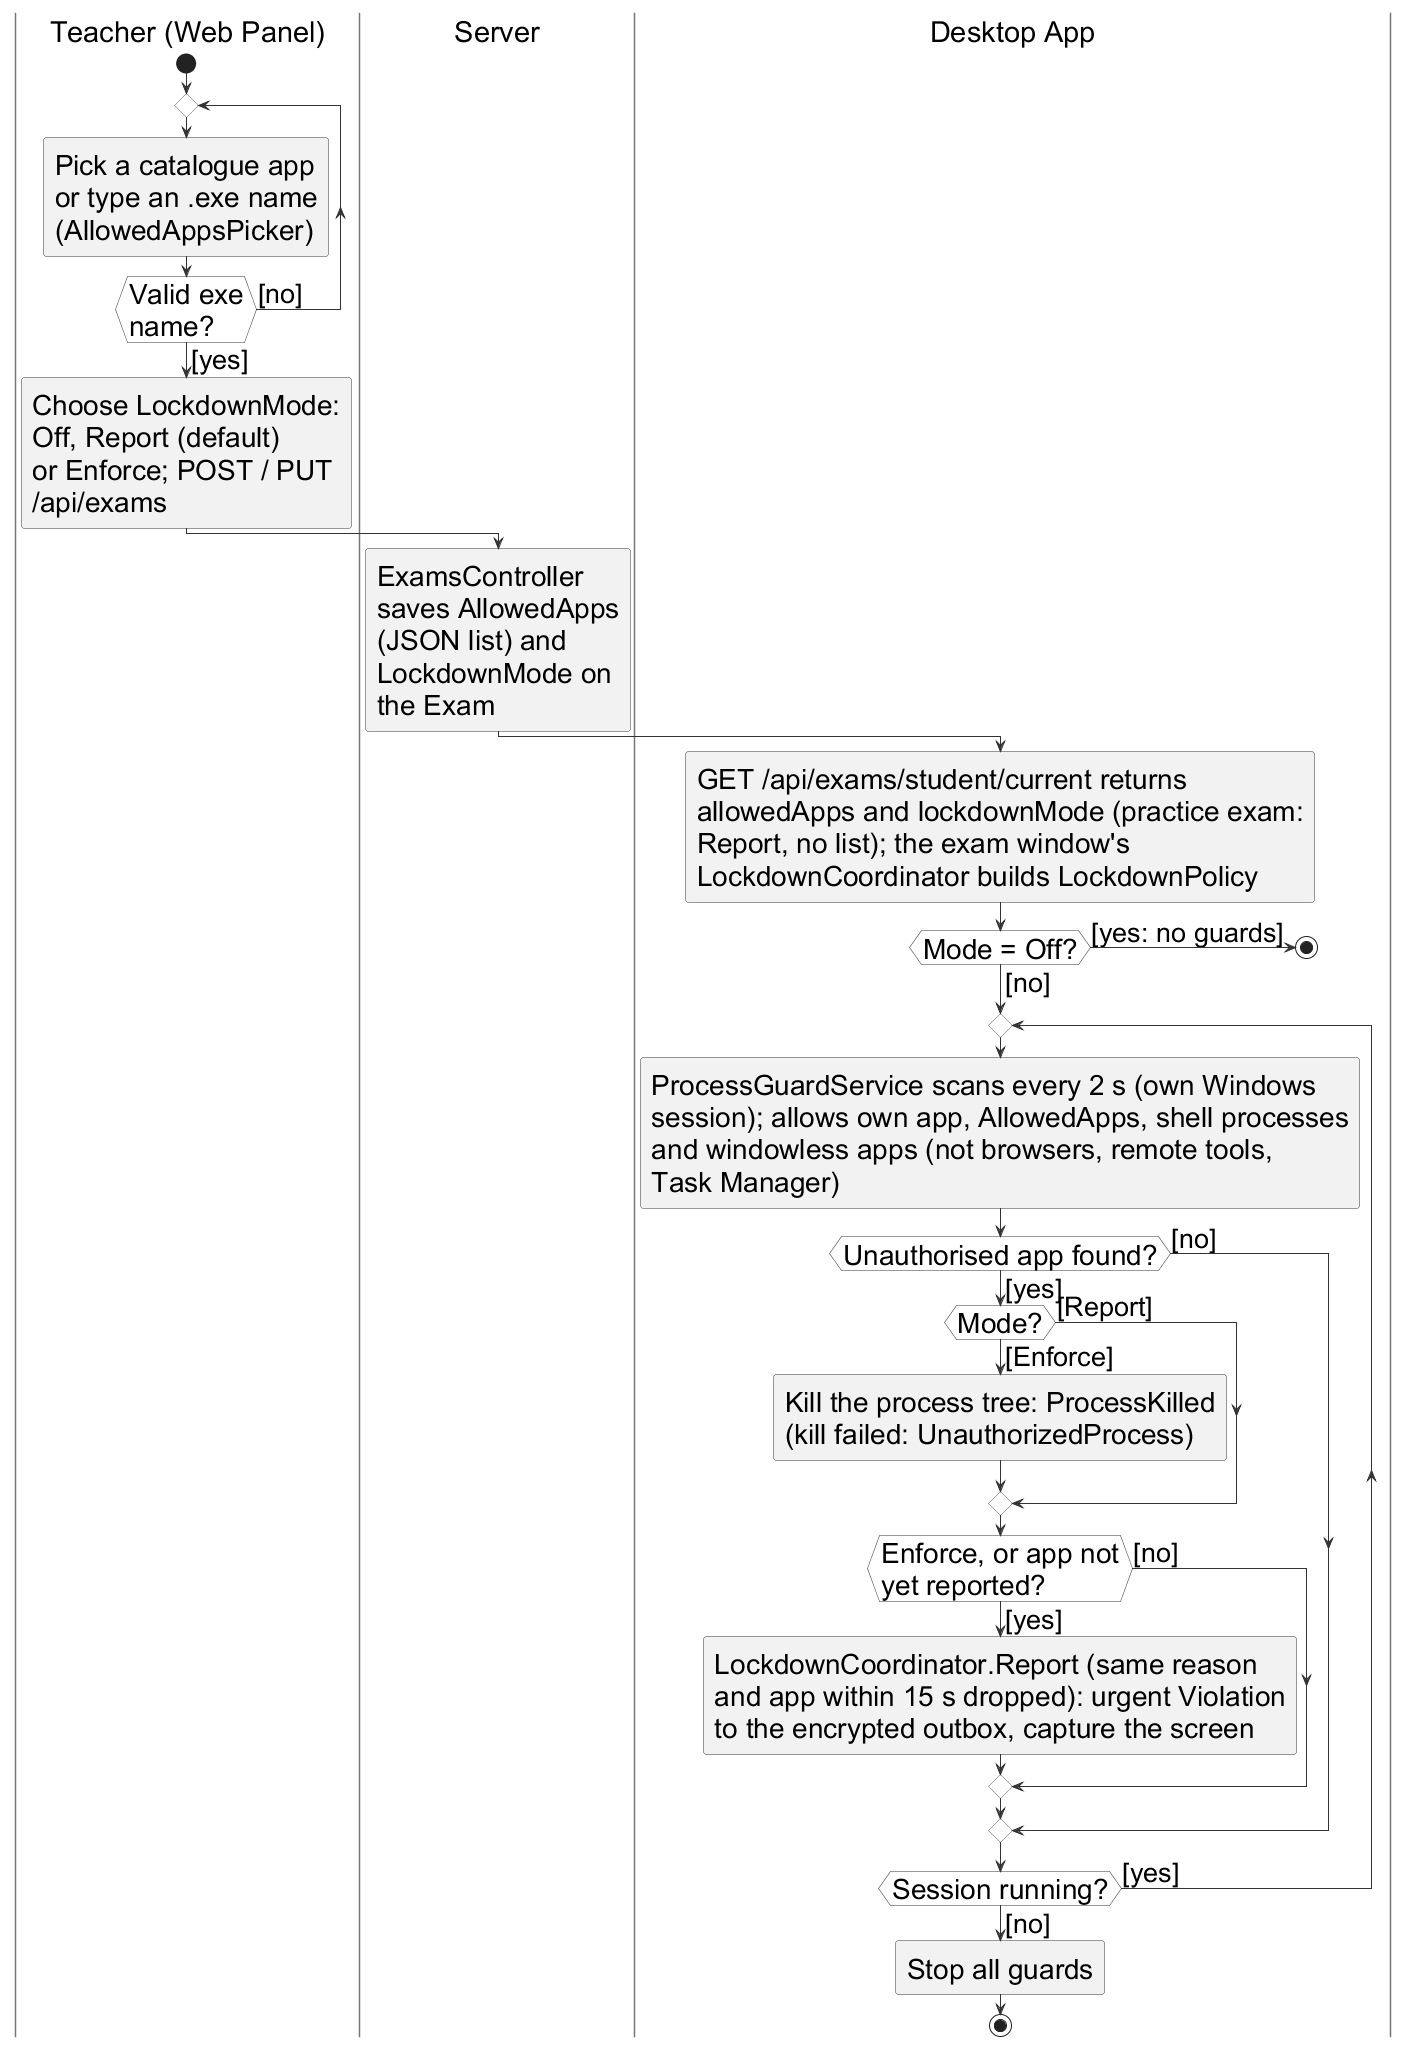
\includegraphics[width=\linewidth,height=562pt,keepaspectratio]{Figures/activity_applications.png}
\caption{Activity Diagram of Allowed Applications Configuration and Enforcement}
\label{fig:activity_applications}
\end{figure}

\subsubsection{Seating and Live Monitoring (M9, M10; UC-04, UC-05, UC-10, UC-11, UC-15, UC-26)}
\begin{sloppypar}
Admins register lab workstations (machine number, host name, IP address), and the teacher or an admin assigns one to each student on the Eligibility page (Figure~\ref{fig:activity_seating}). A start from a non-desktop token is refused with \texttt{DESKTOP\_CLIENT\_REQUIRED}. When \texttt{Exam.EnforceSeat} is on, \texttt{SeatGuard} compares the machine name or IP with the assigned seat; a mismatch blocks the start with \texttt{SEAT\_MISMATCH} and alerts the invigilators on the live monitor, and each heartbeat re-checks the seat.
\end{sloppypar}

\begin{figure}[p]
\centering
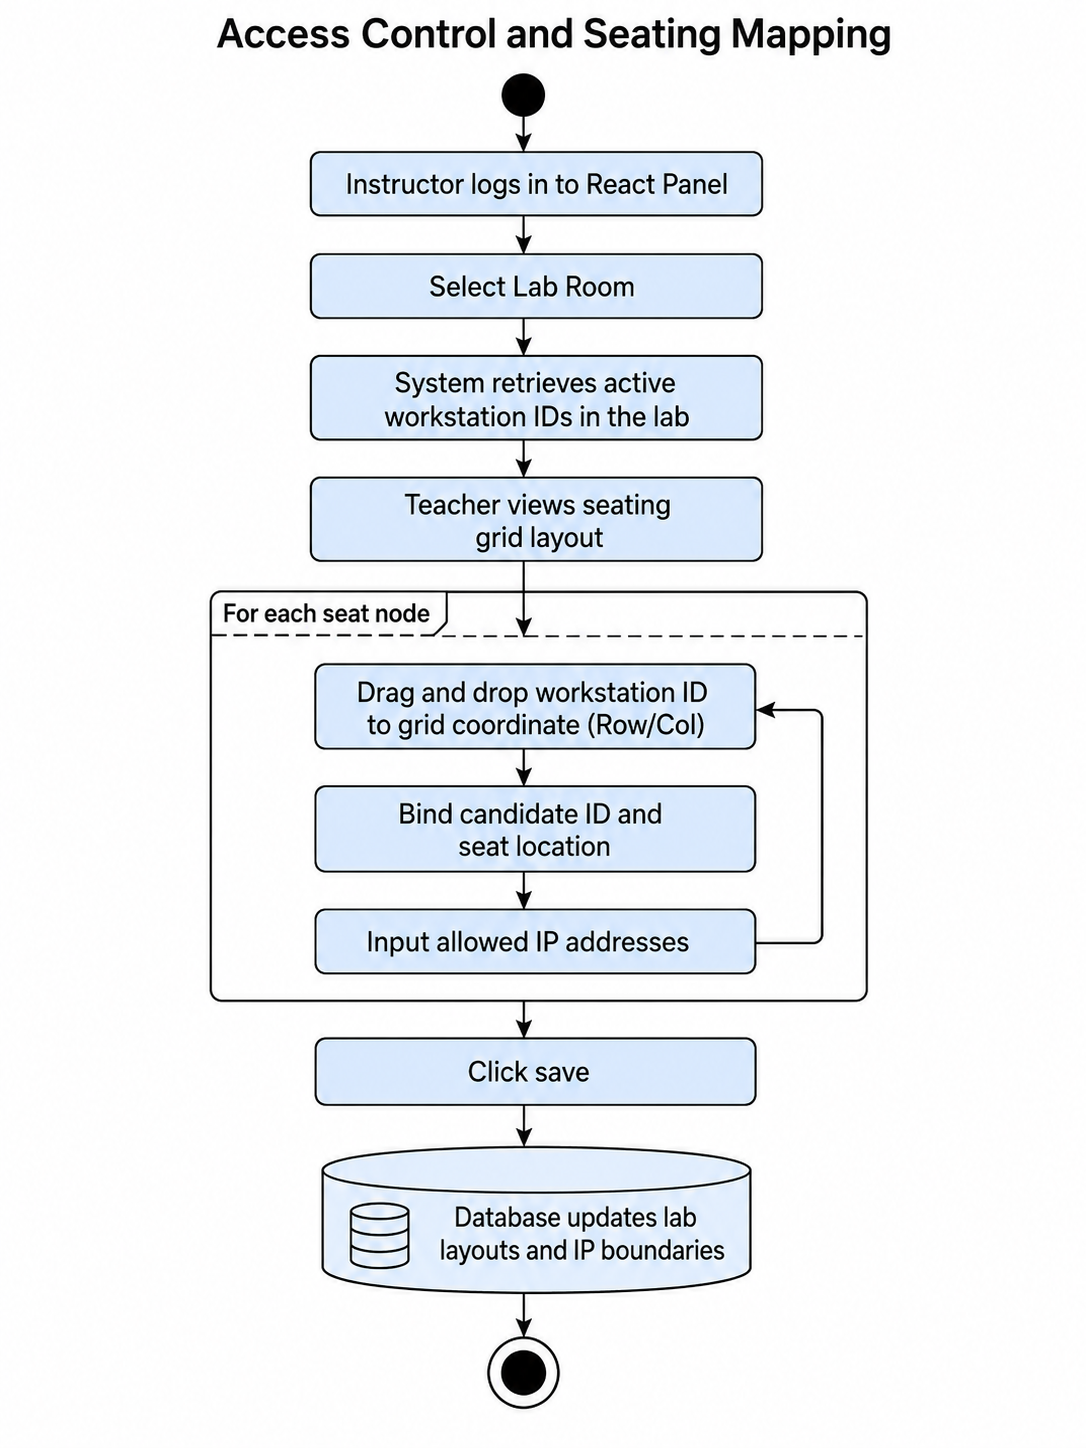
\includegraphics[width=\linewidth,height=628pt,keepaspectratio]{Figures/activity_seating.png}
\caption{Activity Diagram of Seat Assignment}
\label{fig:activity_seating}
\end{figure}

\DiagramBarrier
\begin{sloppypar}
In Figure~\ref{fig:activity_monitoring} the live monitor page joins the exam's group on \texttt{MonitoringHub}. Clients send heartbeats, event batches, screenshots and, when \texttt{RequireWebcam} is on, webcam snapshots over REST to \texttt{MonitoringController}, which stores them, audits violations as \texttt{MONITORING\_VIOLATION} and pushes them to the page. Each tile's status (Stable, Warning, Suspicious or Critical) comes from \texttt{ViolationClassifier}. Staff can warn a student, extend their time, unlock the PC or force-submit, and the client learns the result from its next heartbeat reply. \texttt{HeartbeatWatchdogService} marks a session disconnected after 30 seconds without a heartbeat and audits \texttt{SESSION\_DISCONNECTED}.
\end{sloppypar}

\begin{sidewaysfigure}
\centering
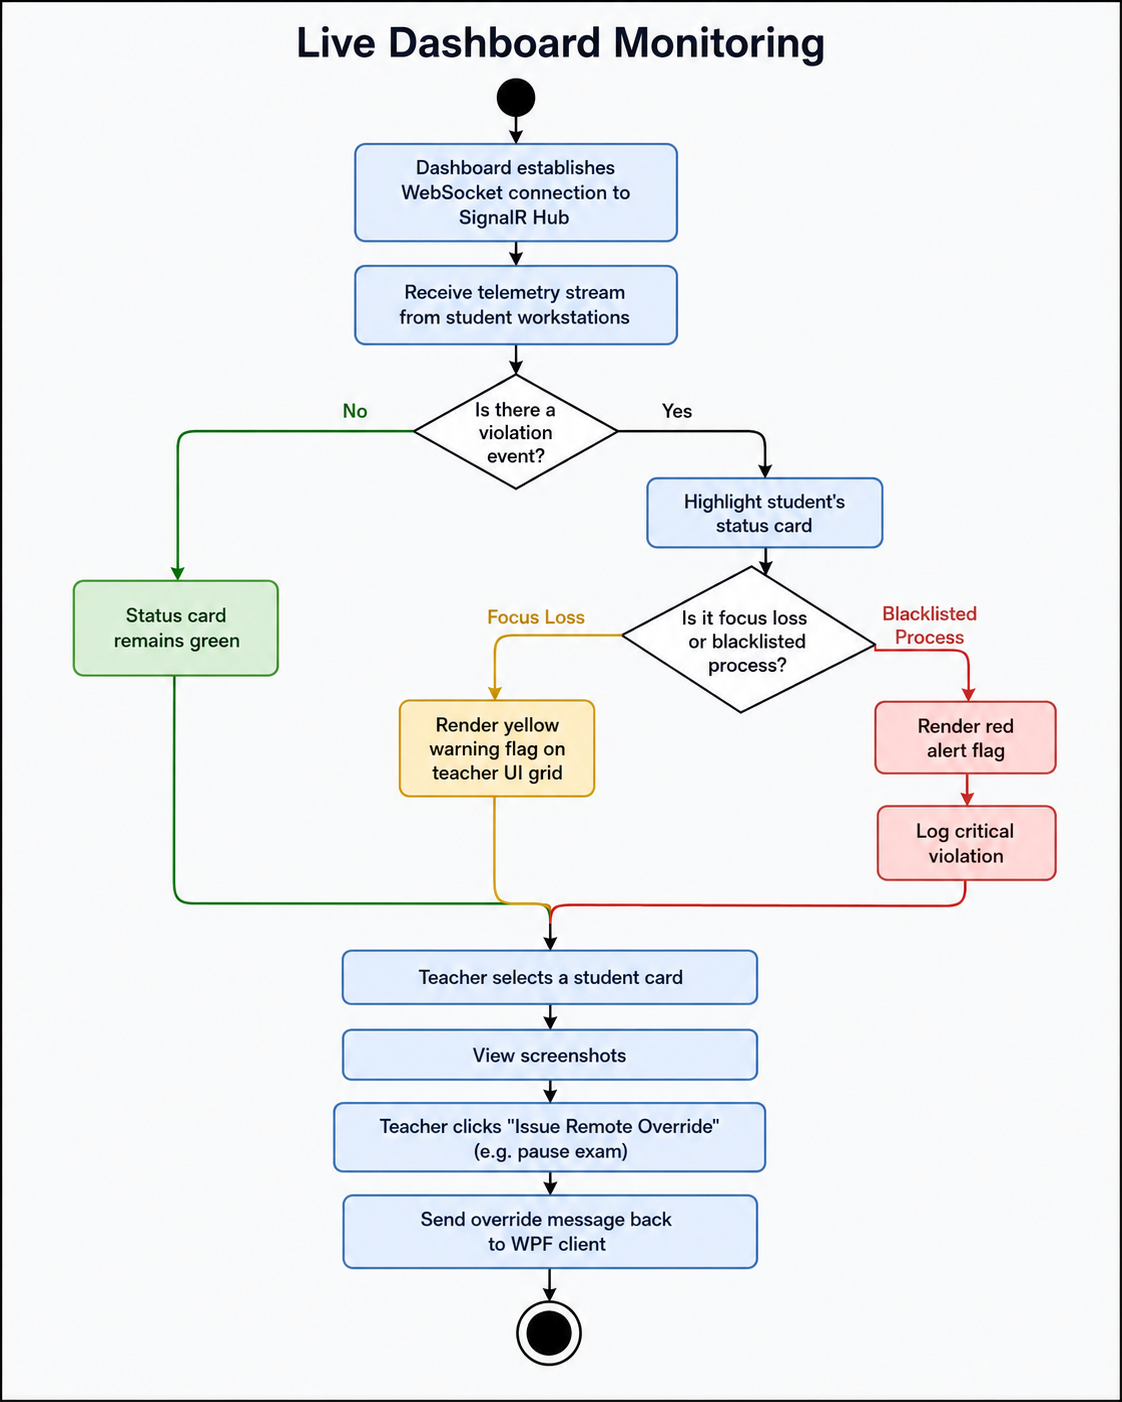
\includegraphics[width=\linewidth,height=0.85\textwidth,keepaspectratio]{Figures/activity_monitoring.png}
\caption{Activity Diagram of Live Monitoring}
\label{fig:activity_monitoring}
\end{sidewaysfigure}

\subsubsection{Grading, Reports and Audit (M11, M12; UC-16 to UC-18, UC-21)}
\begin{sloppypar}
After submission (Figure~\ref{fig:activity_grading}) MCQ answers are checked against the key, and theory answers are scored by TF-IDF \cite{salton1988} (0.7 cosine similarity plus 0.3 key-term coverage) or queued for the optional LLM grader. Plagiarism is checked pairwise with $k$-gram winnowing \cite{winnowing} ($k = 5$ tokens, window $w = 4$, so any shared run of 8 tokens is found) for non-practice exams. \texttt{GradingWorker} then hands each queued coding answer to \texttt{GradingService}, which runs it against its test cases \cite{alamutka2005} in Docker \texttt{gcc:13} (no network) or the MinGW fallback (not isolated); without a runner the answer is left for teacher review. The teacher can accept all suggested marks at once, which skips answers that need a manual mark, or override or regrade a single answer.
\end{sloppypar}

\begin{figure}[p]
\centering
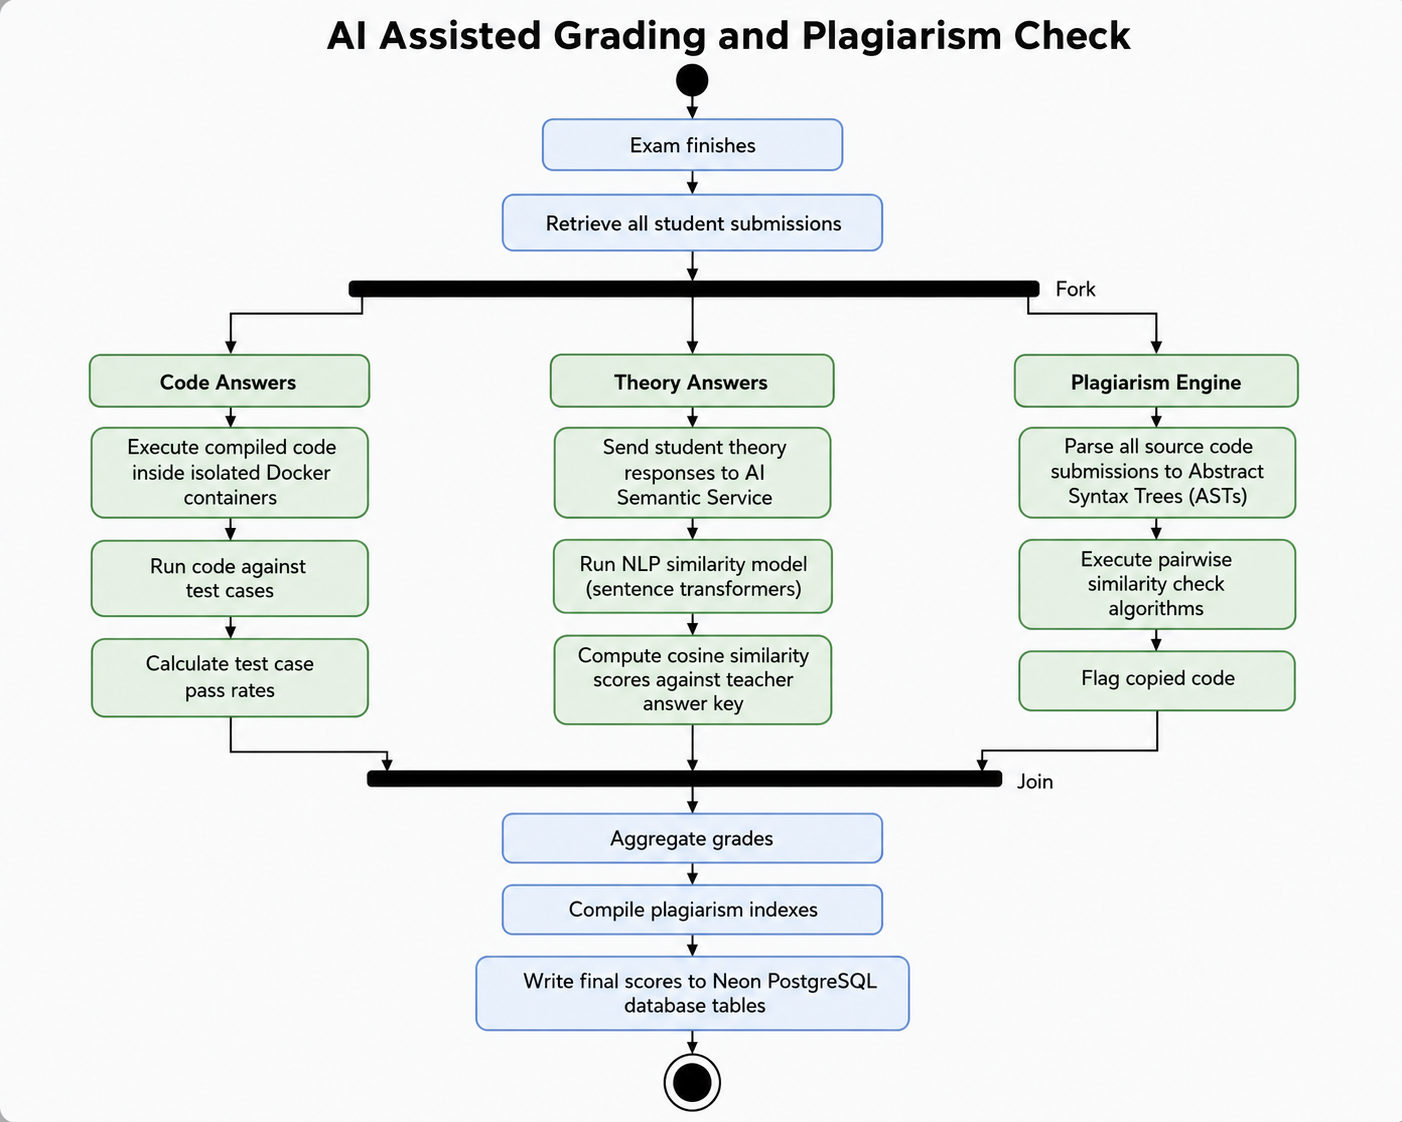
\includegraphics[width=\linewidth,height=628pt,keepaspectratio]{Figures/activity_grading.png}
\caption{Activity Diagram of AI-Assisted Grading and Plagiarism Check}
\label{fig:activity_grading}
\end{figure}

For an exam summary report (Figure~\ref{fig:activity_report}) the API renders a QuestPDF document with summary statistics, per-question performance and the score distribution, records it in \texttt{ExamReports} and returns a download link; this summary is not audited. The attendance, violations and scores PDFs, the Excel file and the evidence ZIP are produced by \texttt{ReportExportService} and audited as \texttt{REPORT\_GENERATED} with the file's SHA-256.

\begin{figure}[H]
\centering
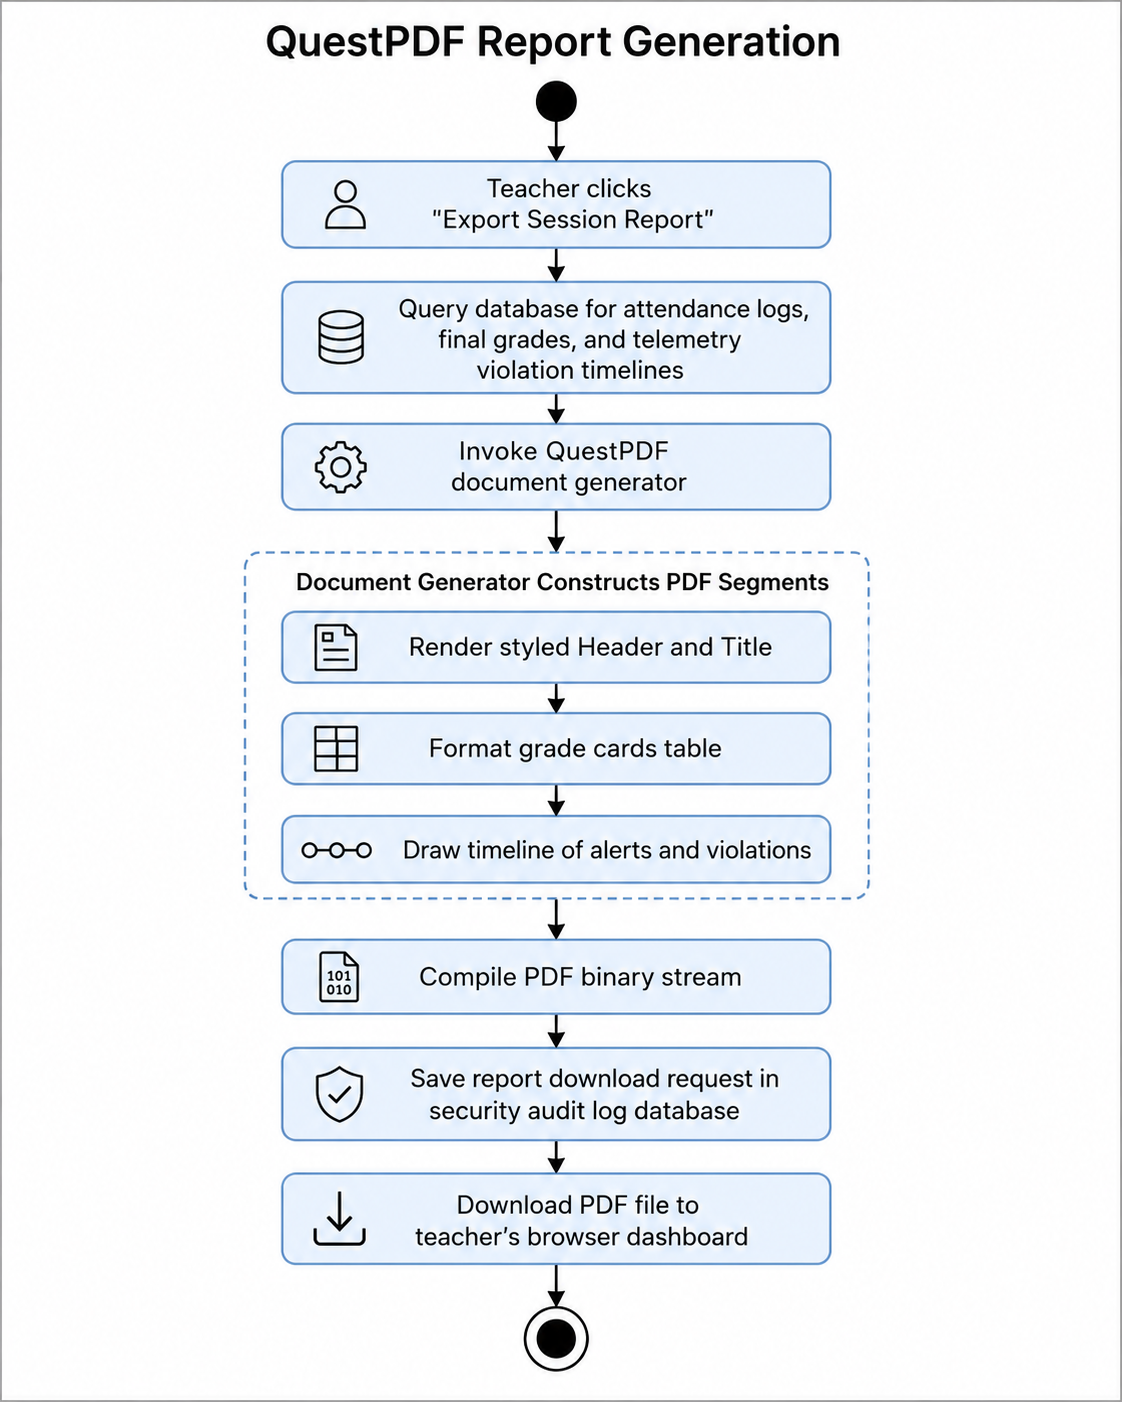
\includegraphics[width=0.90\linewidth,height=446pt,keepaspectratio]{Figures/activity_report.png}
\caption{Activity Diagram of Exam Summary Report Generation}
\label{fig:activity_report}
\end{figure}

Controllers, the hub and services write audit entries through \texttt{AuditService}: standalone events (refused logins, device mismatches, synced violation batches) are saved at once, and the rest are staged with the change they record. \texttt{SaveChanges} then seals each new row into a hash chain (sequence number, previous hash, SHA-256 of the row), one writer at a time, and admins read the log and its verification status on the audit page (Figure~\ref{fig:activity_audit}). Rows written before the chain existed show as not sealed until an admin runs the backfill (\texttt{POST} \url{/api/audit-logs/backfill}, audited as \texttt{AUDIT\_CHAIN\_BACKFILLED}).

\begin{figure}[p]
\centering
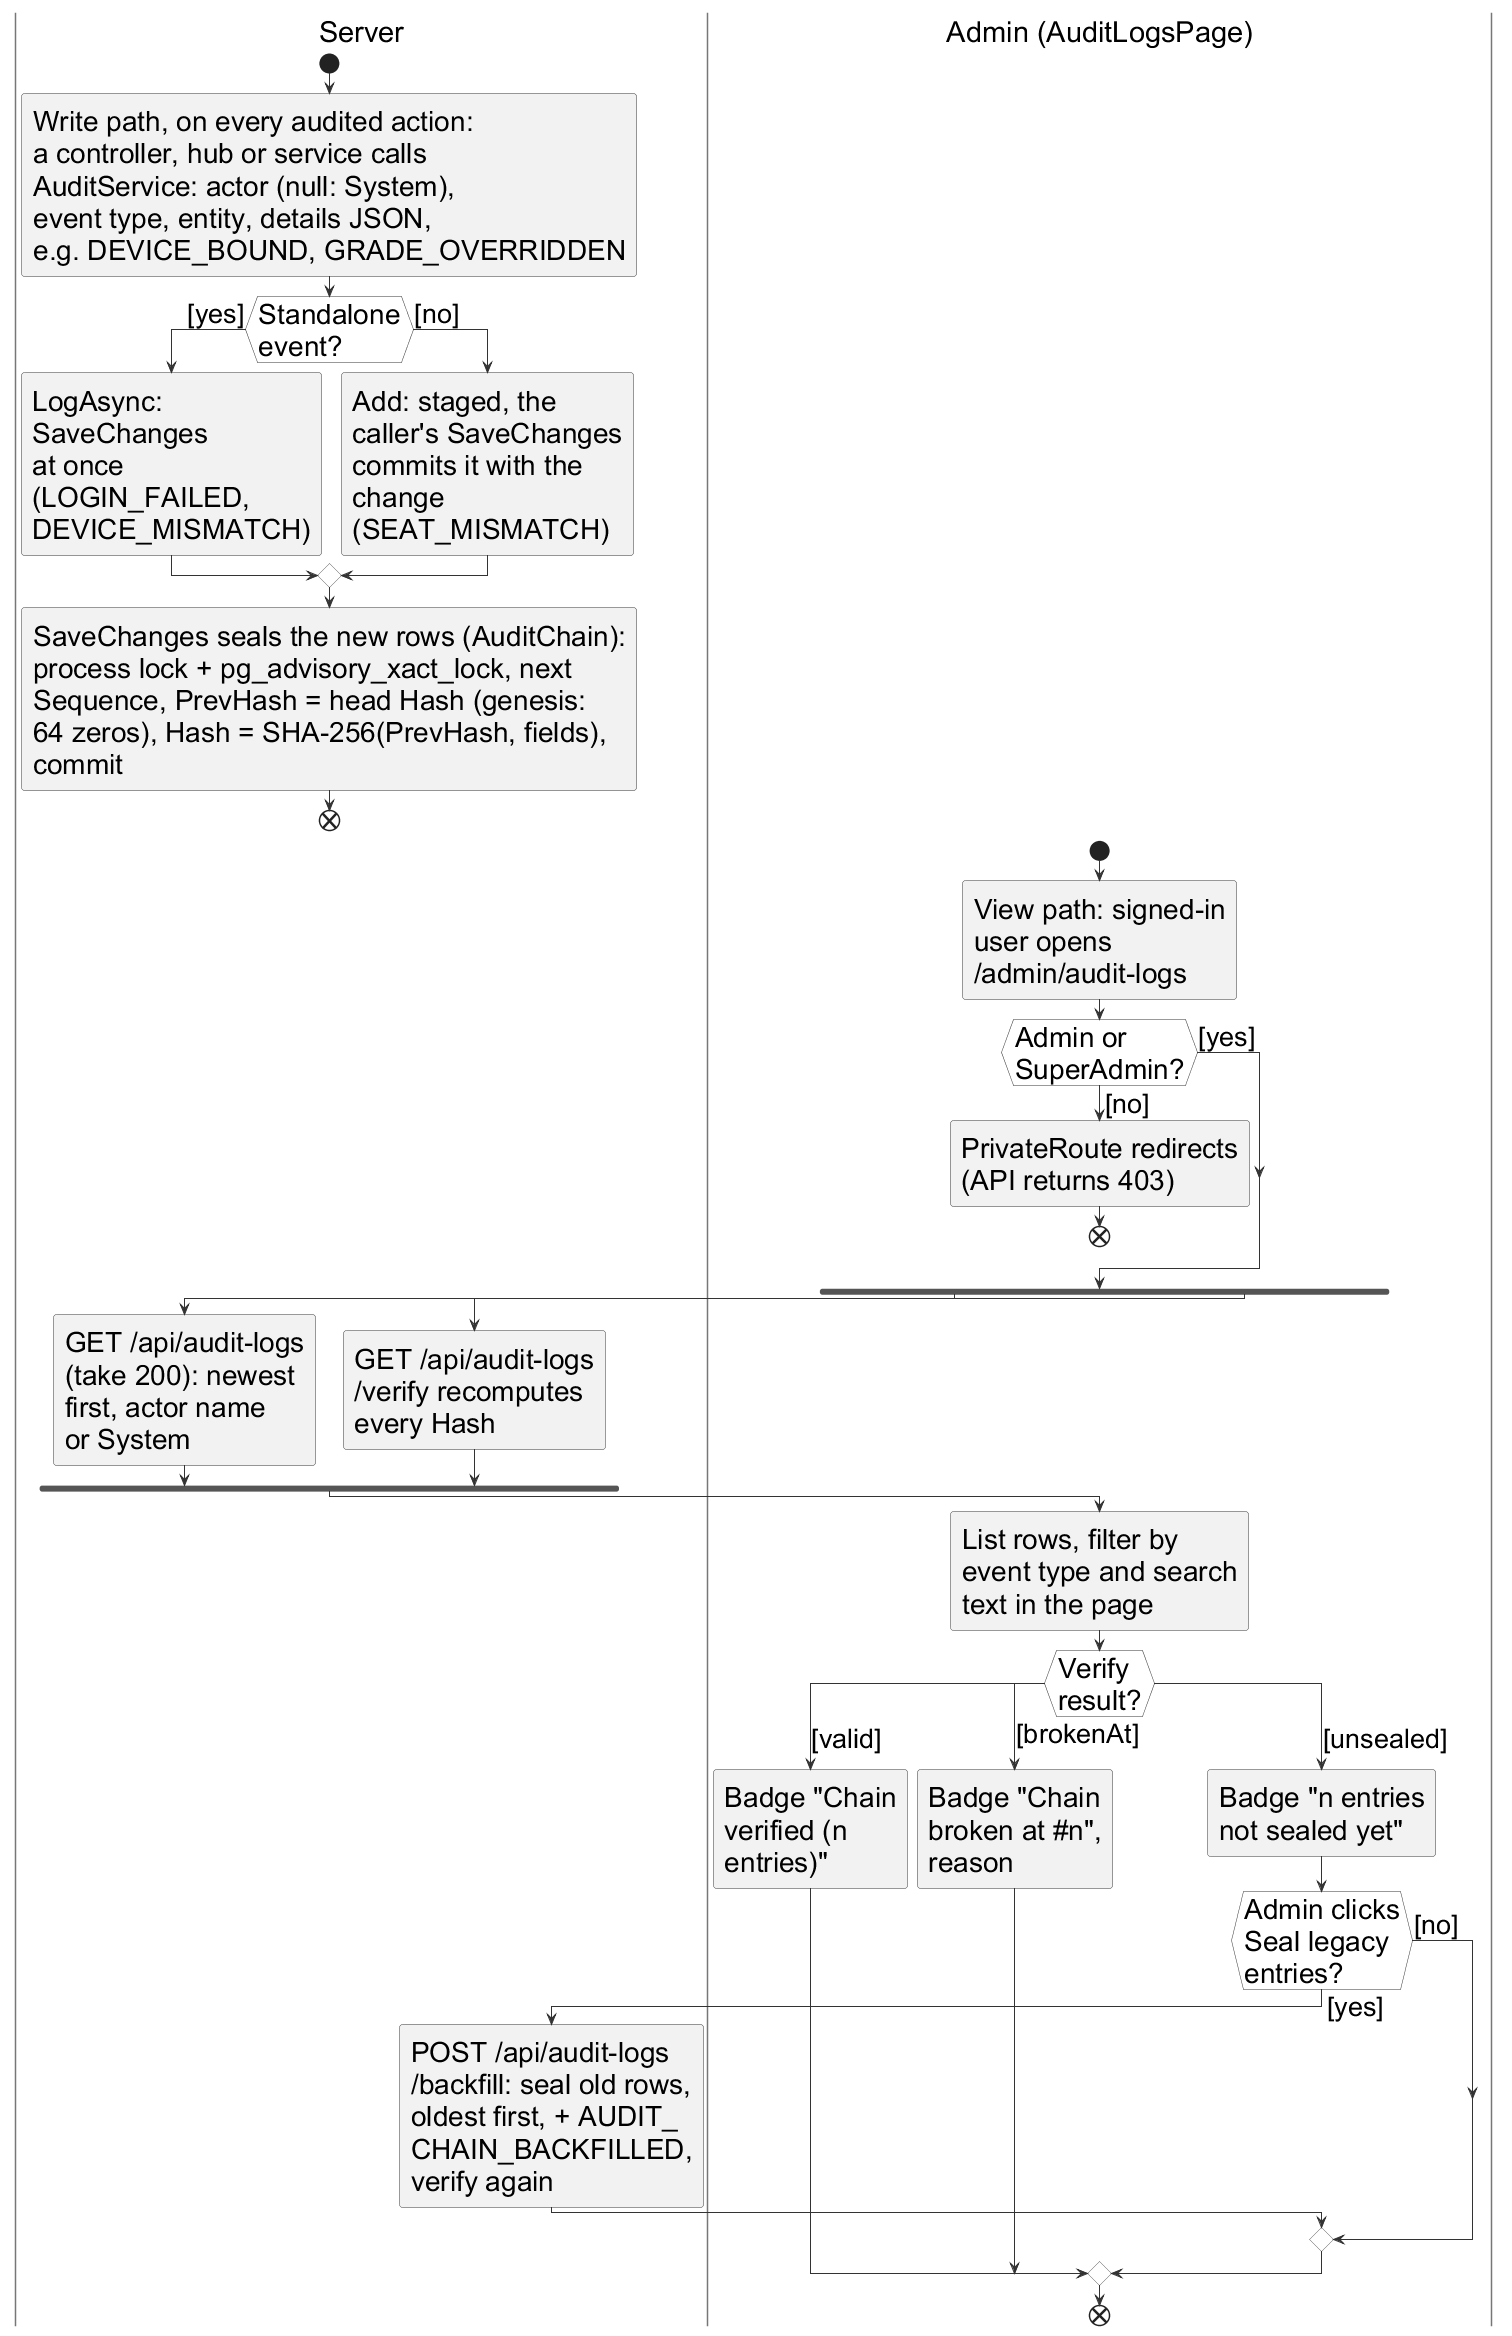
\includegraphics[width=\linewidth,height=628pt,keepaspectratio]{Figures/activity_audit.png}
\caption{Activity Diagram of Audit Logging}
\label{fig:activity_audit}
\end{figure}

\DiagramBarrier
\subsection{Communication Diagram}
\begin{sloppypar}
A communication diagram shows the objects in one interaction and their numbered messages \cite[Cl.~17.9]{omg_uml251}. Figure~\ref{fig:communication_diagram} follows a violation: the client posts it over REST, and \texttt{MonitoringController} stores it and pushes it through the hub to the live monitor (messages 1--1.1.2). A teacher or invigilator acts on the page (2), which calls the hub with a warning (2.1) or a force-submit (2.2). The hub checks the caller with \texttt{ExamAccessService} and audits the action; a force-submit calls \texttt{SubmissionService.FinalizeAsync}. The client picks up the warning or the new session status from its next heartbeat reply \mbox{(3--4.1)}, and the warning repeats until it is marked read.
\end{sloppypar}

\begin{sidewaysfigure}
\centering
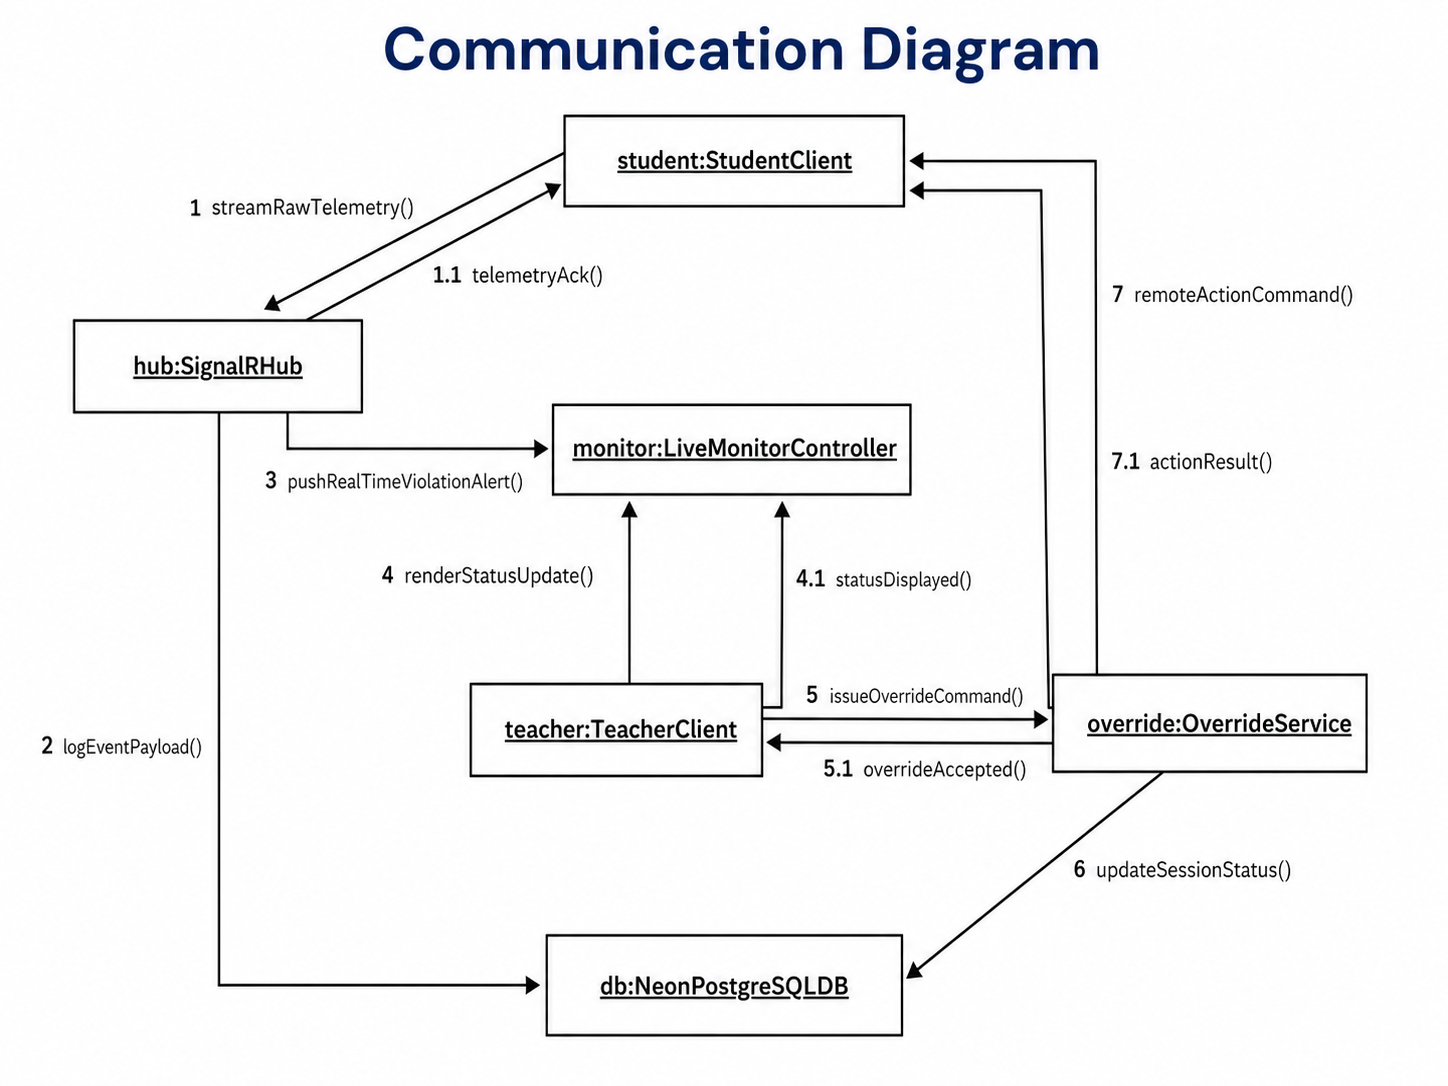
\includegraphics[width=\linewidth,height=415pt,keepaspectratio]{Figures/communication_diagram.png}
\caption{Communication Diagram of Violation Alerts and Staff Response}
\label{fig:communication_diagram}
\end{sidewaysfigure}

\subsection{Sequence Diagrams}
\begin{sloppypar}
A sequence diagram shows the messages between participants in time order \cite[Cl.~17.8]{omg_uml251}, \cite{sequence_diagram_vp}. Filled arrowheads are synchronous calls with dashed replies; open arrowheads are asynchronous messages such as SignalR pushes and queue hand-offs. A desktop lifeline that calls a controller does so through \texttt{ApiClient}, which some diagrams merge into the caller to save width; web-panel lifelines are React pages, not classes.
\end{sloppypar}

\subsubsection{Login, Token Refresh, Logout and Password Change (M1; UC-01, UC-12)}
\begin{sloppypar}
In Figures~\ref{fig:seq_login} and~\ref{fig:seq_login_b} \texttt{AuthController} checks the salted PBKDF2 hash \cite{rfc8018} of the password (600,000 iterations of HMAC-SHA256, as the Open Worldwide Application Security Project (OWASP) recommends \cite{owasp_pwd}), the Student role, the HWID and the device binding (first bind, upgrade of a v1 binding, or \texttt{DEVICE\_MISMATCH}), then returns a JWT \cite{rfc7519} and a refresh token. Because each hash stores its scheme and cost, an older hash is re-hashed at the next login \cite{nist80063b}.
\end{sloppypar}

\DiagramBarrier
\begin{figure}[H]
\centering
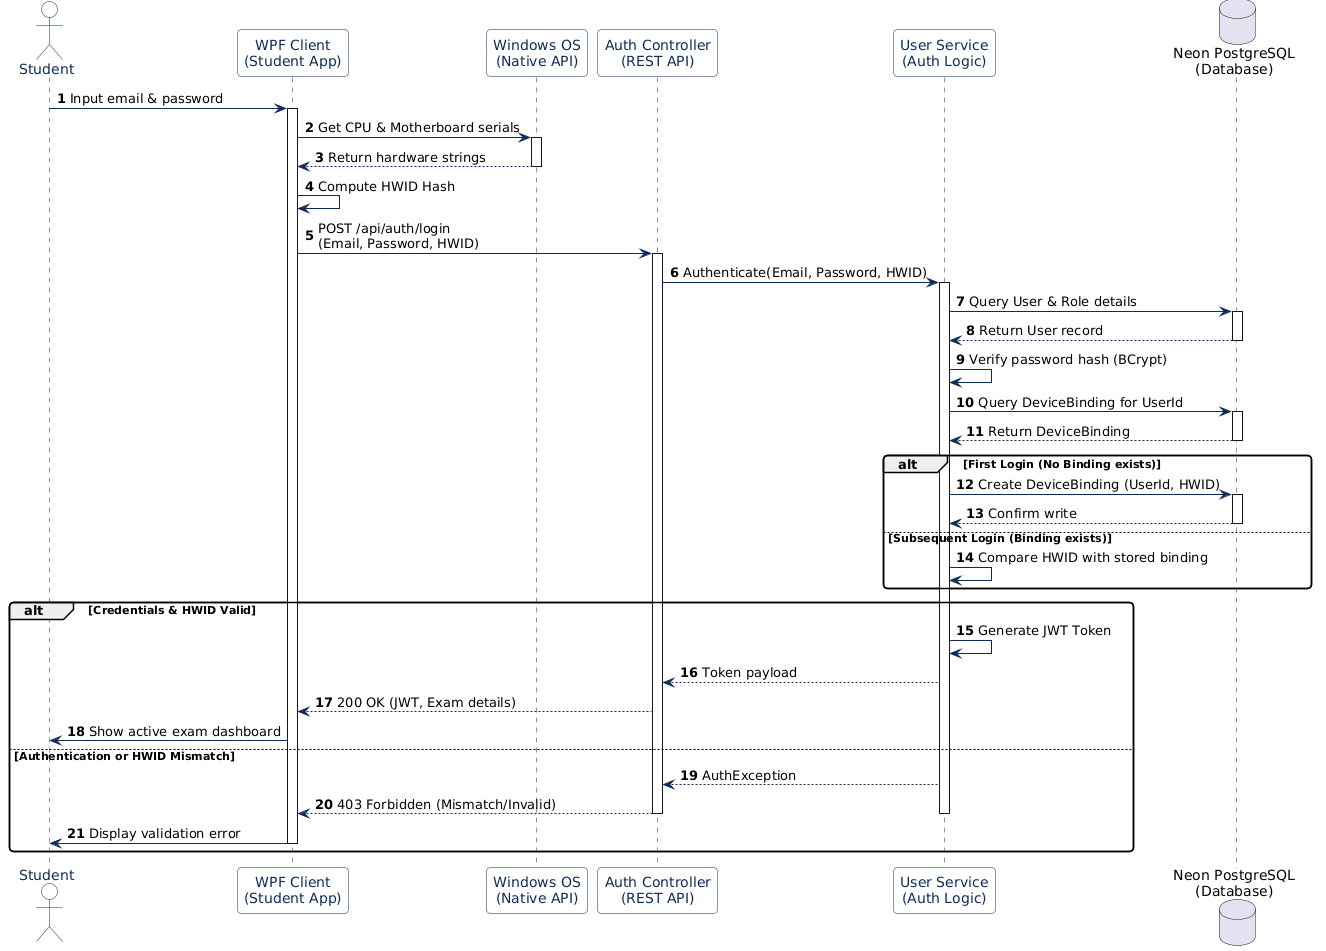
\includegraphics[width=0.85\linewidth,height=443pt,keepaspectratio]{Figures/seq_login.png}
\caption{Sequence Diagram of Student Login and HWID Verification (a): Credential, Role and HWID Checks}
\label{fig:seq_login}
\end{figure}

\begin{figure}[H]
\centering
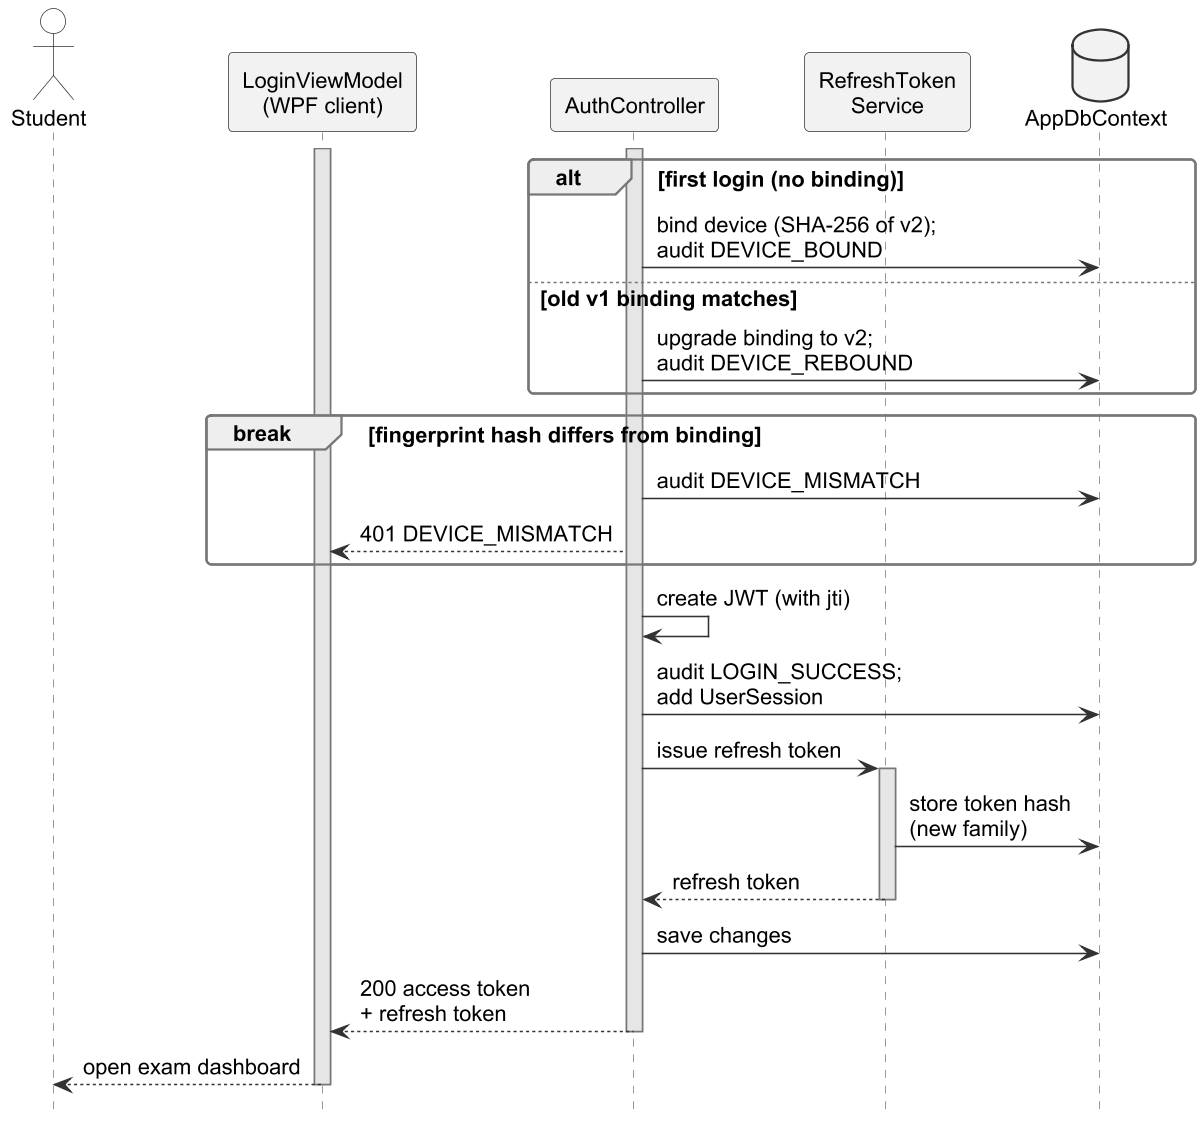
\includegraphics[width=\linewidth,height=446pt,keepaspectratio]{Figures/seq_login_b.png}
\caption{Sequence Diagram of Student Login and HWID Verification (b): Device Binding and Tokens}
\label{fig:seq_login_b}
\end{figure}

Refresh tokens rotate on every use; reusing an old one revokes its whole family \cite[Sec.~4.14.2]{rfc9700} (Figures~\ref{fig:seq_logout} and~\ref{fig:seq_logout_b}). Logout revokes the refresh-token family and the session on the server and audits \texttt{LOGOUT}.

\begin{figure}[H]
\centering
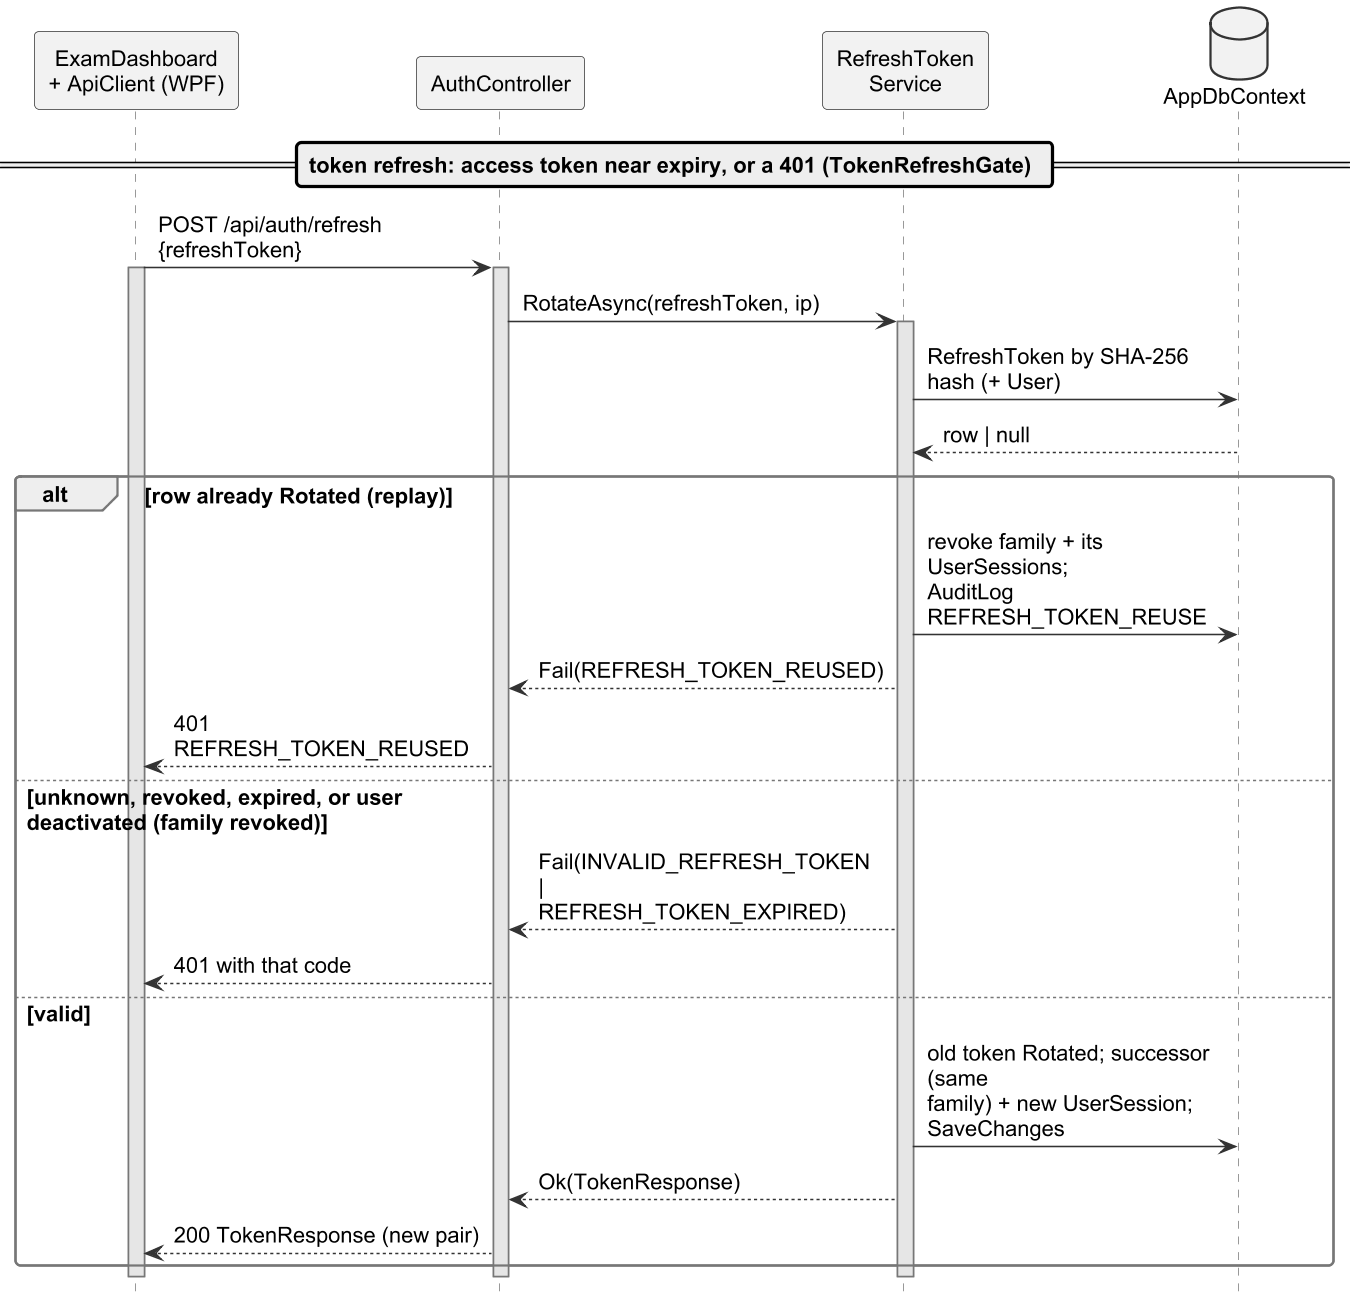
\includegraphics[width=\linewidth,height=432pt,keepaspectratio]{Figures/seq_logout.png}
\caption{Sequence Diagram of Token Refresh and Logout (a): Token Refresh}
\label{fig:seq_logout}
\end{figure}

\begin{figure}[H]
\centering
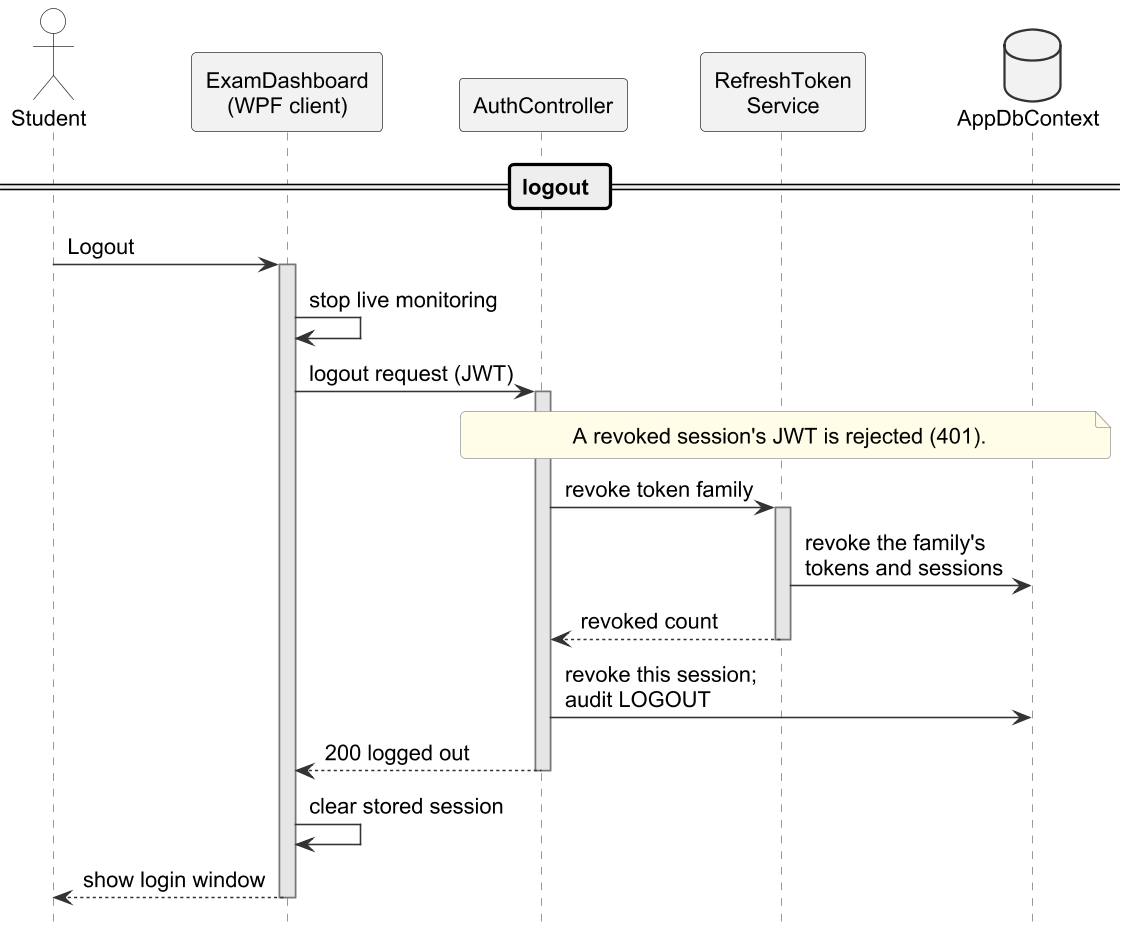
\includegraphics[width=\linewidth,height=361pt,keepaspectratio]{Figures/seq_logout_b.png}
\caption{Sequence Diagram of Token Refresh and Logout (b): Logout}
\label{fig:seq_logout_b}
\end{figure}

\begin{sloppypar}
A staff password change from the web panel (Figures~\ref{fig:seq_change_password} and~\ref{fig:seq_change_password_b}) goes to \url{/api/auth/change-password}, which verifies the current password and a minimum length of 8, ends the user's other sessions, and stores a new salt and PBKDF2 hash; the caller's own session stays valid.
\end{sloppypar}

\begin{figure}[H]
\centering
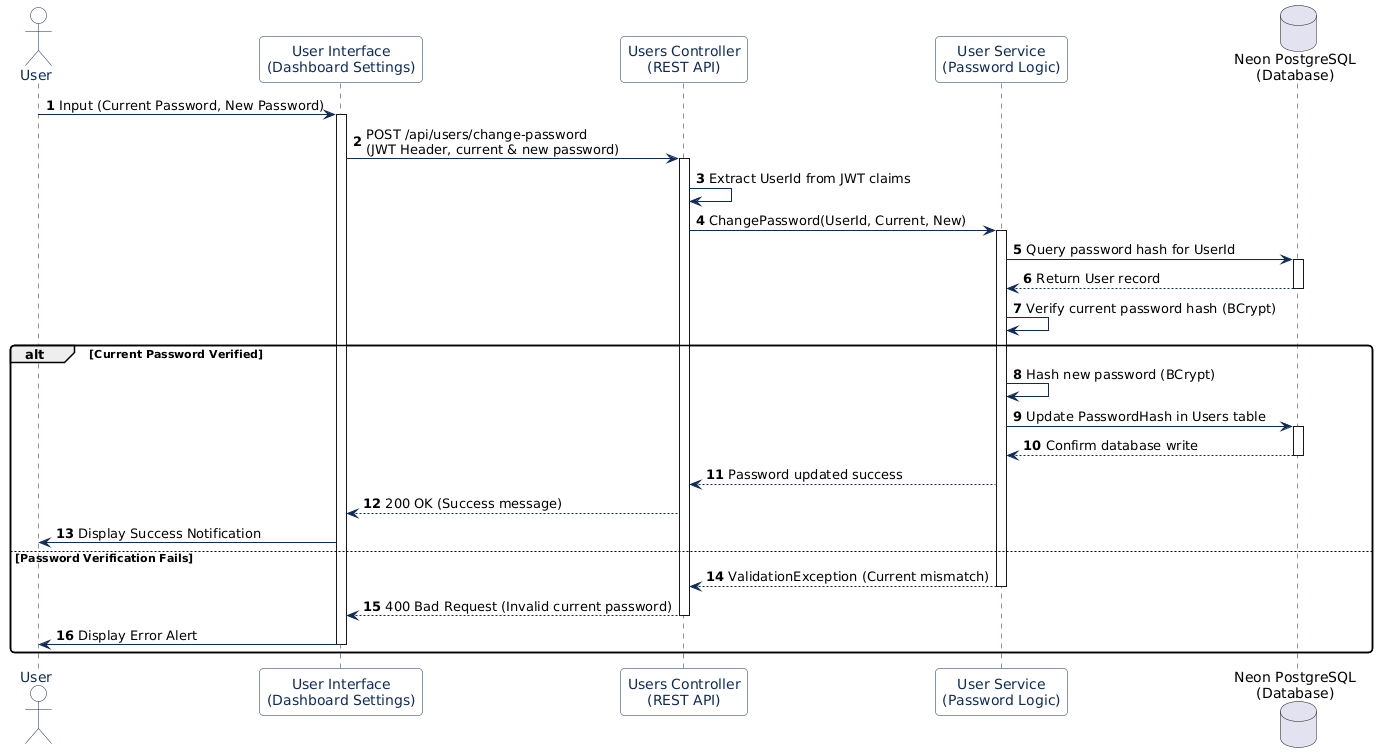
\includegraphics[width=\linewidth,height=388pt,keepaspectratio]{Figures/seq_change_password.png}
\caption{Sequence Diagram of Password Change (a): Request and Password Checks}
\label{fig:seq_change_password}
\end{figure}

\begin{figure}[H]
\centering
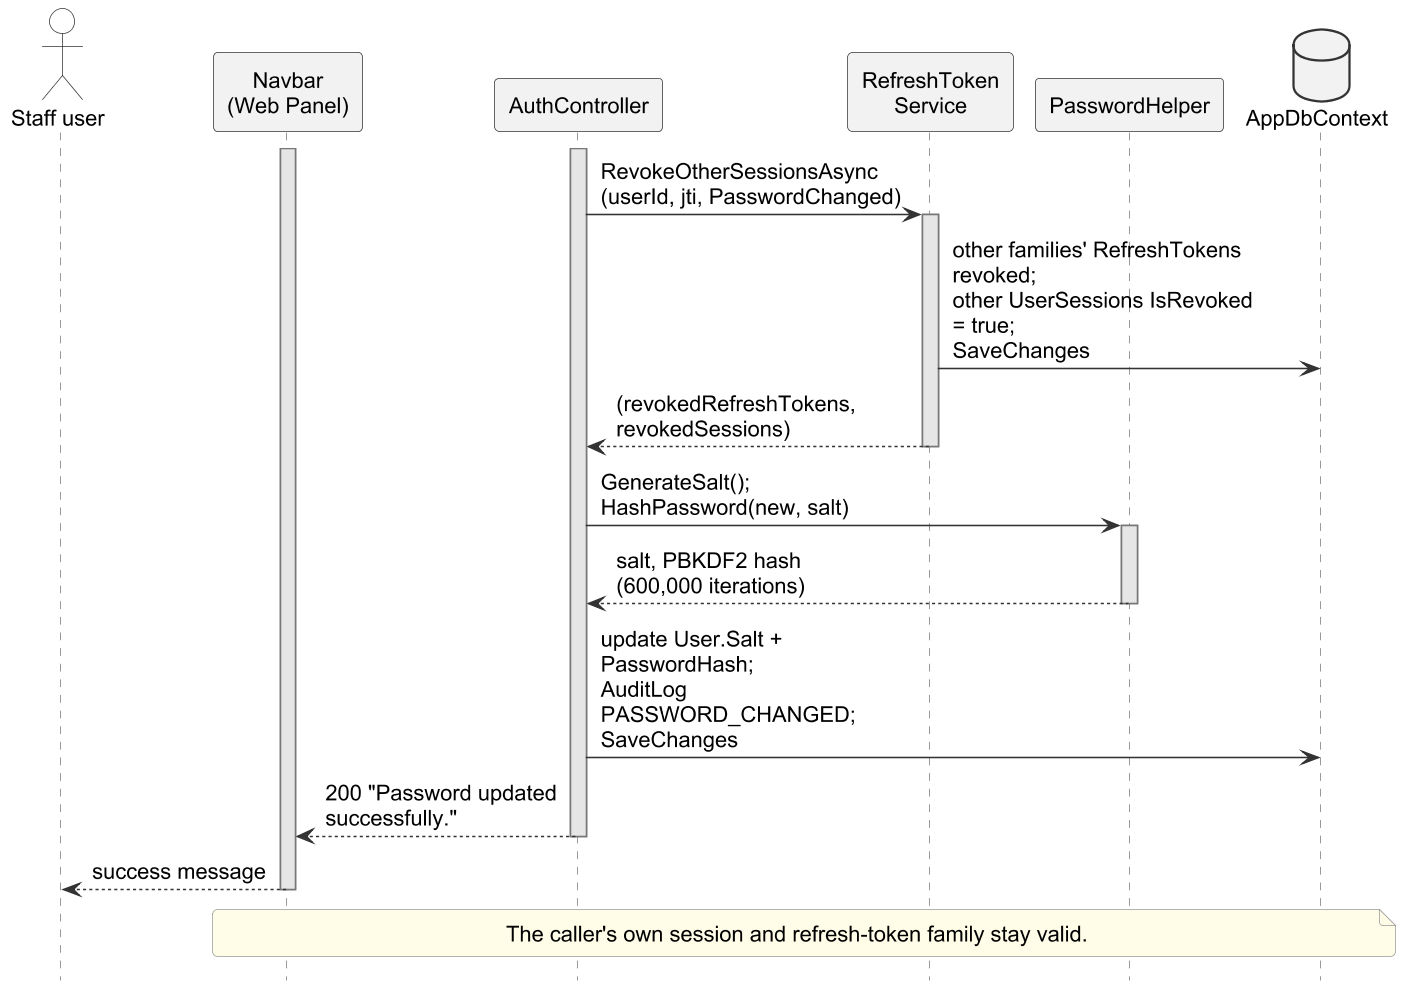
\includegraphics[width=\linewidth,height=318pt,keepaspectratio]{Figures/seq_change_password_b.png}
\caption{Sequence Diagram of Password Change (b): Session Revocation and New Hash}
\label{fig:seq_change_password_b}
\end{figure}

\DiagramBarrier
\subsubsection{Session Timeline and Live Telemetry (M3, M5, M10; UC-04, UC-07, UC-09)}
\begin{sloppypar}
To view a student's record (Figures~\ref{fig:seq_view_database} and~\ref{fig:seq_view_database_b}), staff call \texttt{MonitoringEvidenceController}, which checks access through \texttt{ExamAccessService} (owner teacher, assigned invigilator or admin) and returns the session's events (without heartbeats), screenshots, warnings, incidents and audit entries, newest first; each image is then fetched through \texttt{EvidenceStorage}.
\end{sloppypar}

\begin{figure}[H]
\centering
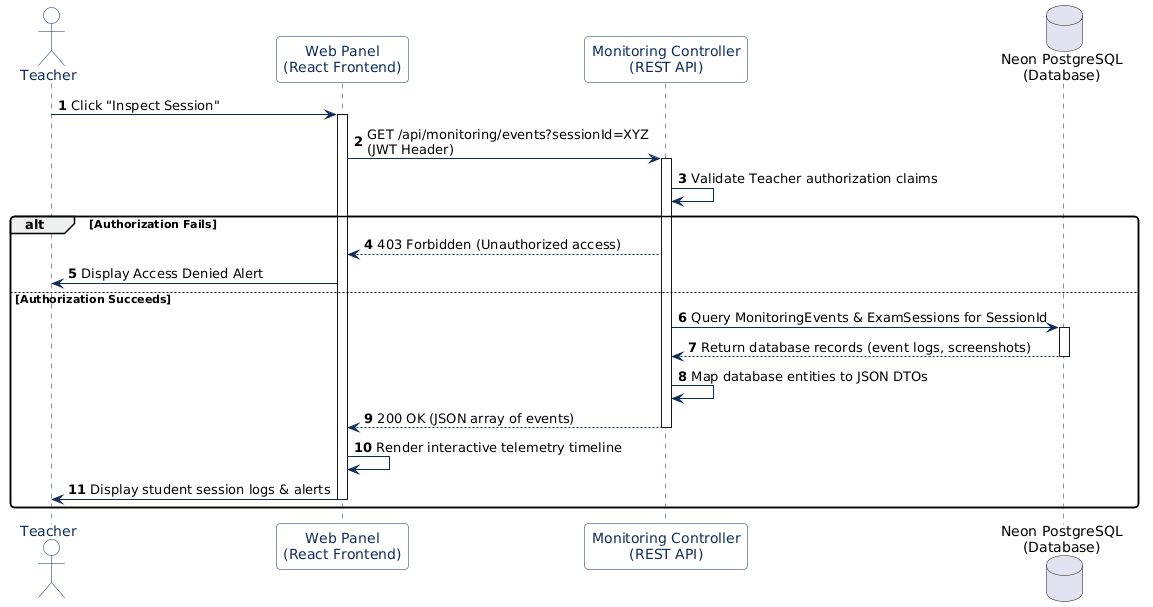
\includegraphics[width=\linewidth,height=439pt,keepaspectratio]{Figures/seq_view_database.png}
\caption{Sequence Diagram of Viewing a Session Timeline (a): Access Check and Timeline}
\label{fig:seq_view_database}
\end{figure}

\begin{figure}[H]
\centering
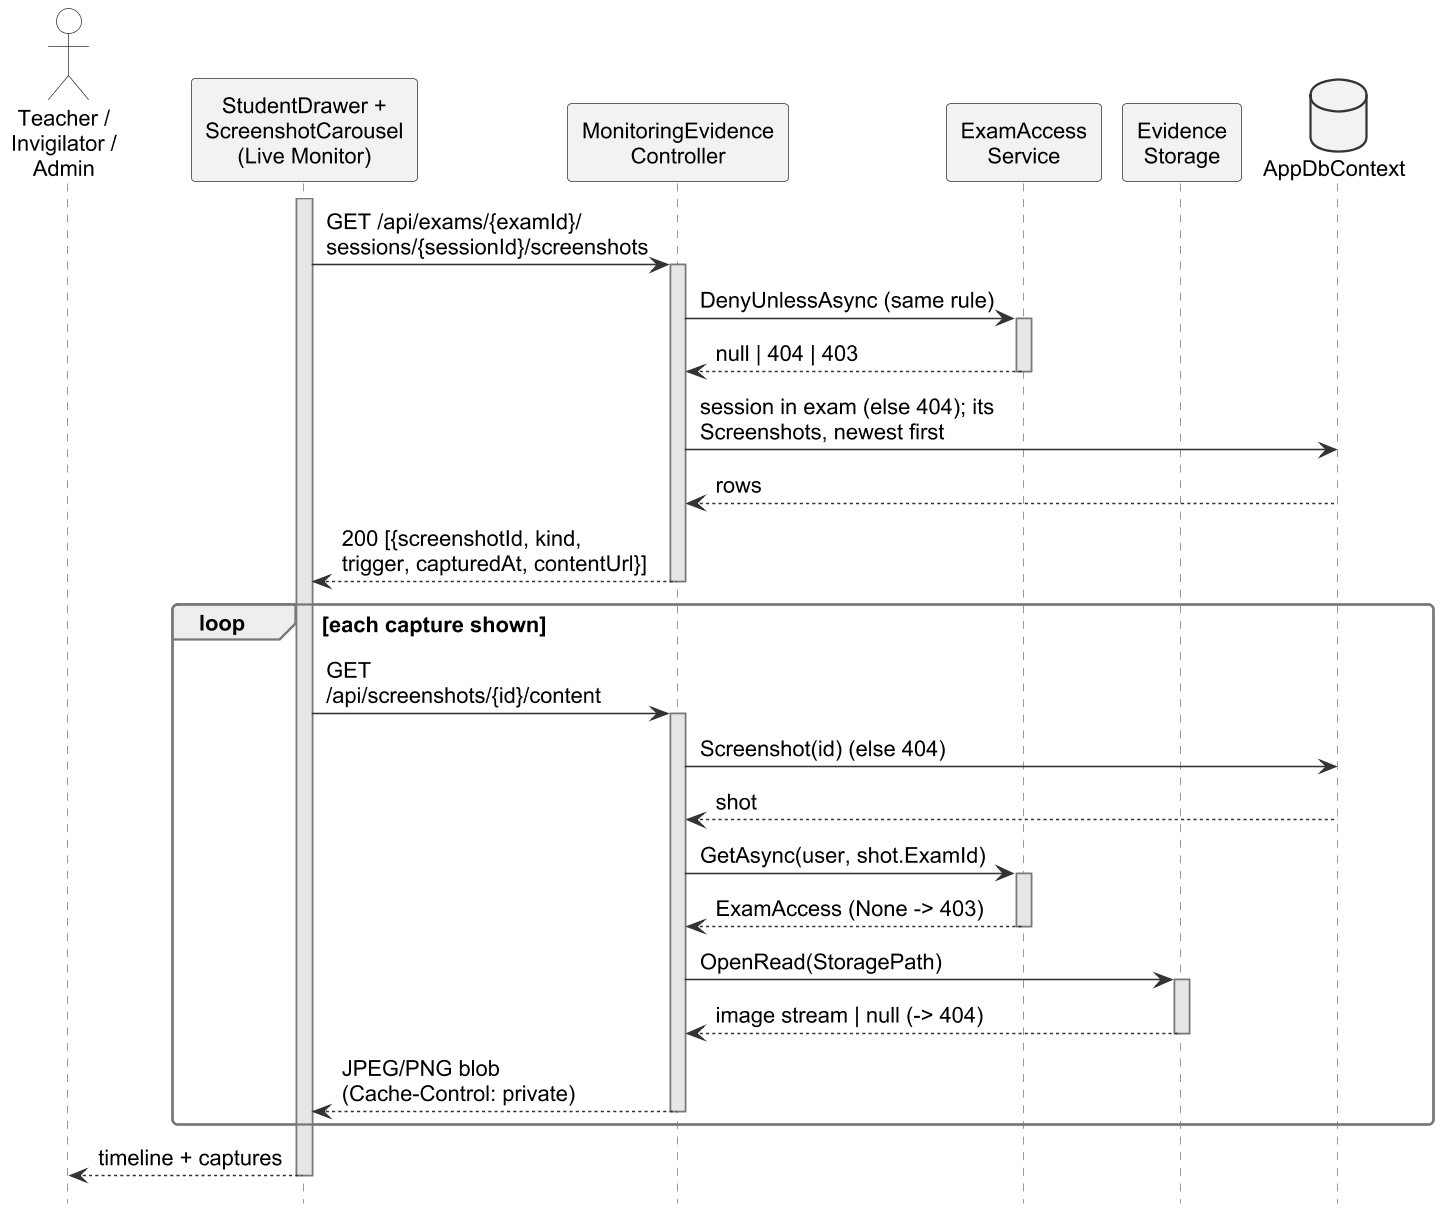
\includegraphics[width=\linewidth,height=380pt,keepaspectratio]{Figures/seq_view_database_b.png}
\caption{Sequence Diagram of Viewing a Session Timeline (b): Capture List and Images}
\label{fig:seq_view_database_b}
\end{figure}

In Figures~\ref{fig:seq_telemetry} and~\ref{fig:seq_telemetry_b} the start call checks the assignment, seat and readiness gates and creates the session. The client then sends a REST heartbeat every 10 seconds and event batches every 5 seconds. Screen captures are uploaded at random intervals around \texttt{ScreenshotIntervalSeconds} (30--90 seconds by default) and after each violation, plus webcam snapshots when \texttt{RequireWebcam} is set. The server pushes these updates to the exam's hub group, and \texttt{HeartbeatWatchdogService} marks a session disconnected after 30 seconds of silence.

\begin{figure}[H]
\centering
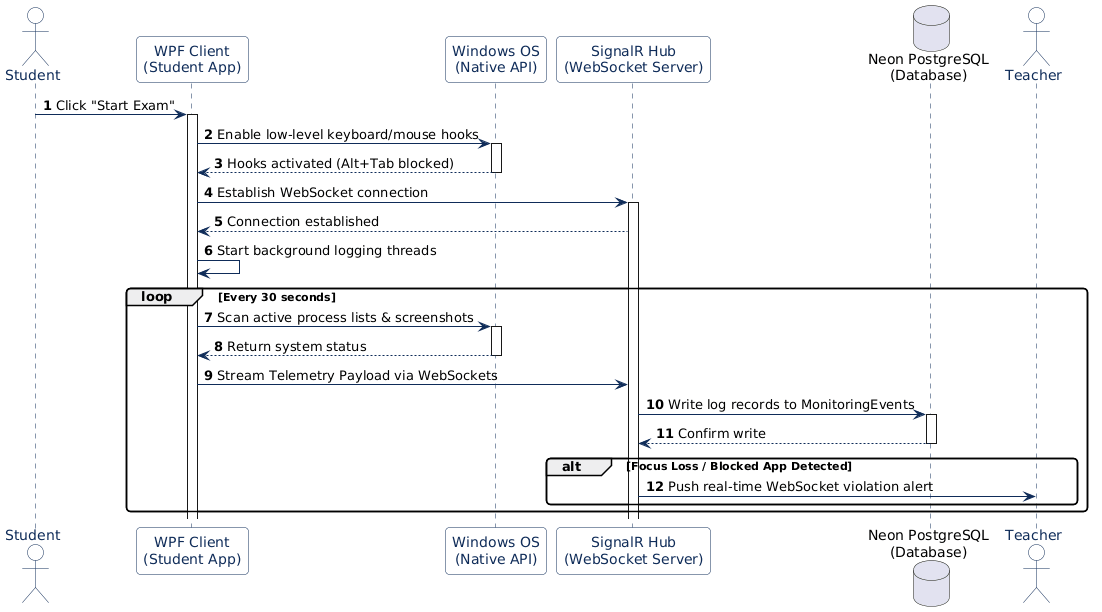
\includegraphics[width=\linewidth,height=473pt,keepaspectratio]{Figures/seq_telemetry.png}
\caption{Sequence Diagram of Exam Start and Telemetry (a): Start, Heartbeats and Event Batches}
\label{fig:seq_telemetry}
\end{figure}

\begin{figure}[H]
\centering
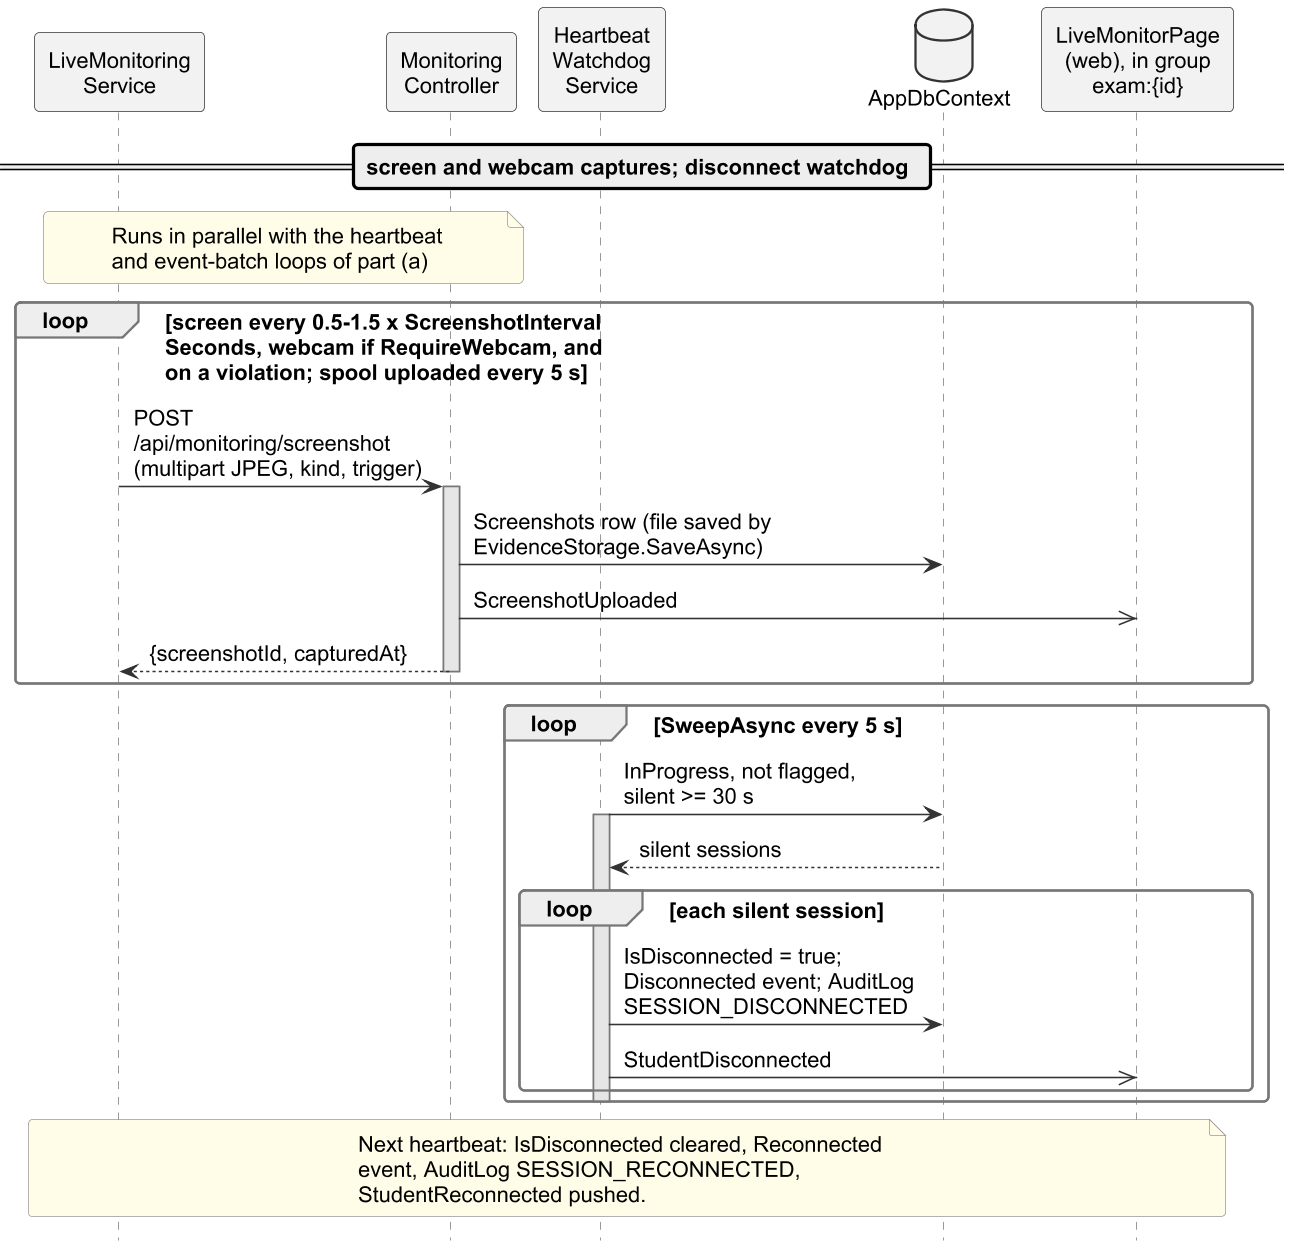
\includegraphics[width=\linewidth,height=436pt,keepaspectratio]{Figures/seq_telemetry_b.png}
\caption{Sequence Diagram of Exam Start and Telemetry (b): Captures and Disconnect Watchdog}
\label{fig:seq_telemetry_b}
\end{figure}

\DiagramBarrier
\subsubsection{Grading, Code Execution and Plagiarism (M11; UC-16, UC-17)}
\begin{sloppypar}
Plagiarism is checked in two places. The teacher's heat map (Figure~\ref{fig:seq_plagiarism_matrix}) compares every pair of students on demand and refuses practice exams. On submit (Figures~\ref{fig:seq_ai_plagiarism} and~\ref{fig:seq_ai_plagiarism_b}) \texttt{FinalizeAsync} stages the answers: MCQ and theory answers are marked at once (theory by the TF-IDF grader unless the LLM grader is on), and coding answers are queued for the code runner unless blank or no runner is configured. For non-practice exams, coding and theory answers are compared pairwise with the same question's answers in other finalised sessions, and pairs at or above the exam's \texttt{PlagiarismThreshold} are stored in \texttt{PlagiarismResults}. The session, marks, pairs and \texttt{SESSION\_SUBMITTED} audit entry are saved together, and the receipt is returned without waiting for code grading.
\end{sloppypar}

\begin{figure}[H]
\centering
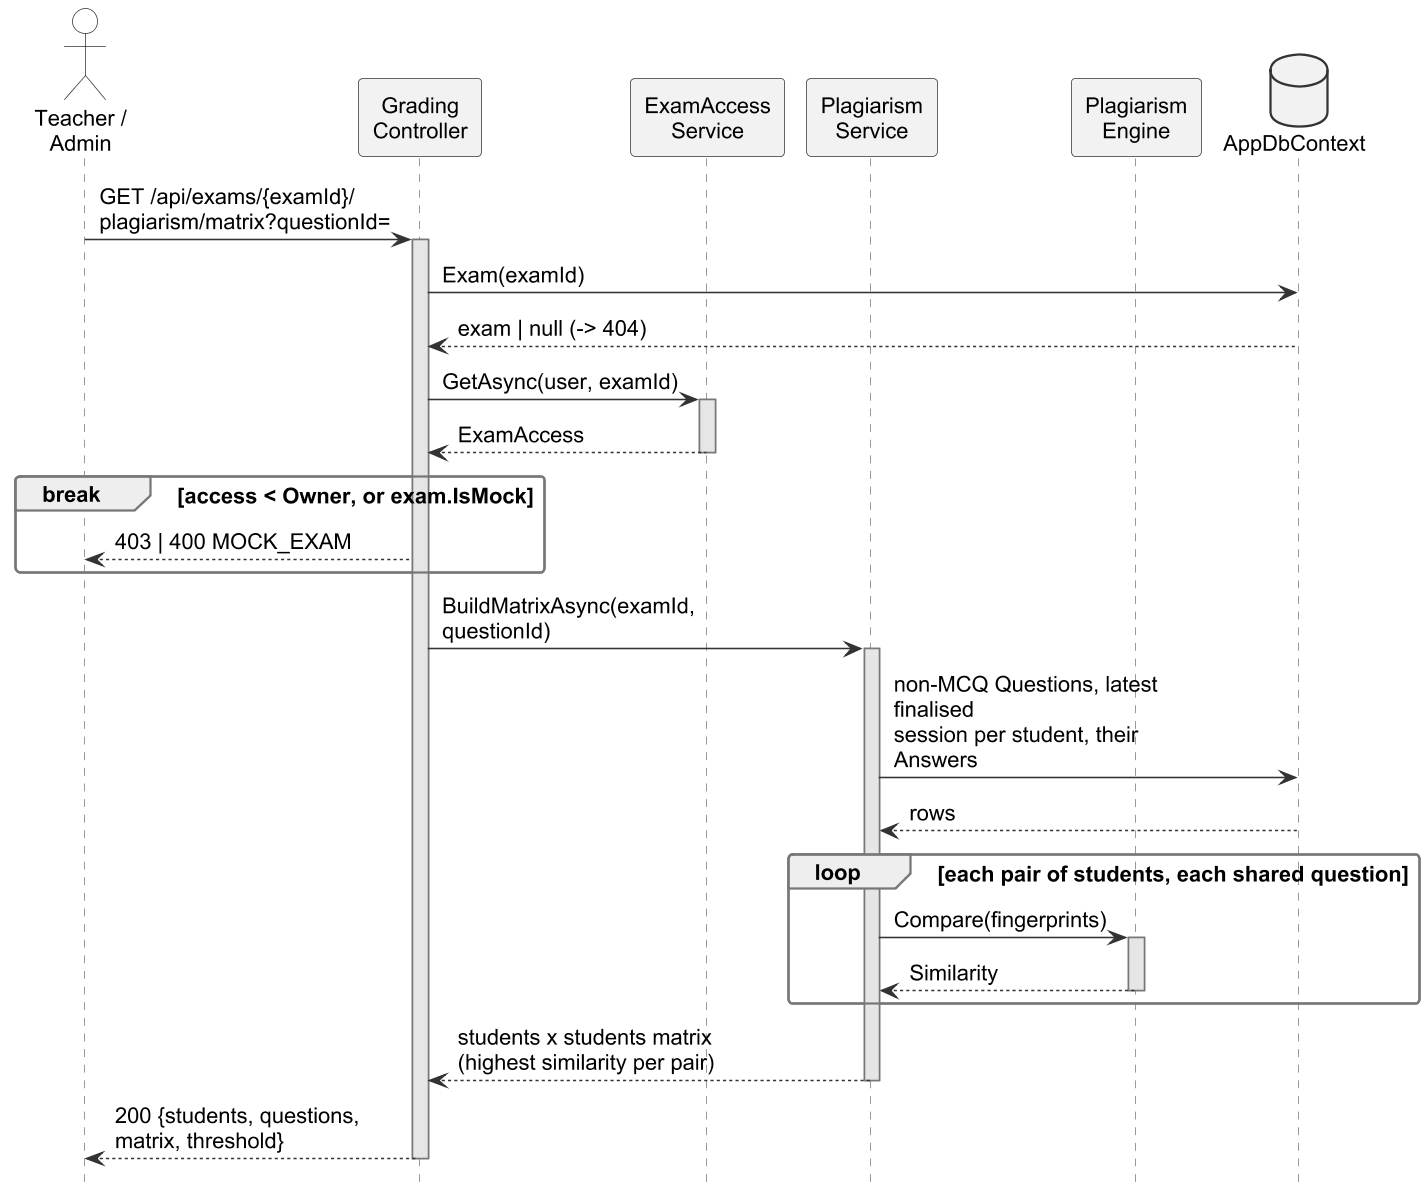
\includegraphics[width=\linewidth,height=378pt,keepaspectratio]{Figures/seq_plagiarism_matrix.png}
\caption{Sequence Diagram of the Plagiarism Heat Map}
\label{fig:seq_plagiarism_matrix}
\end{figure}

\begin{figure}[H]
\centering
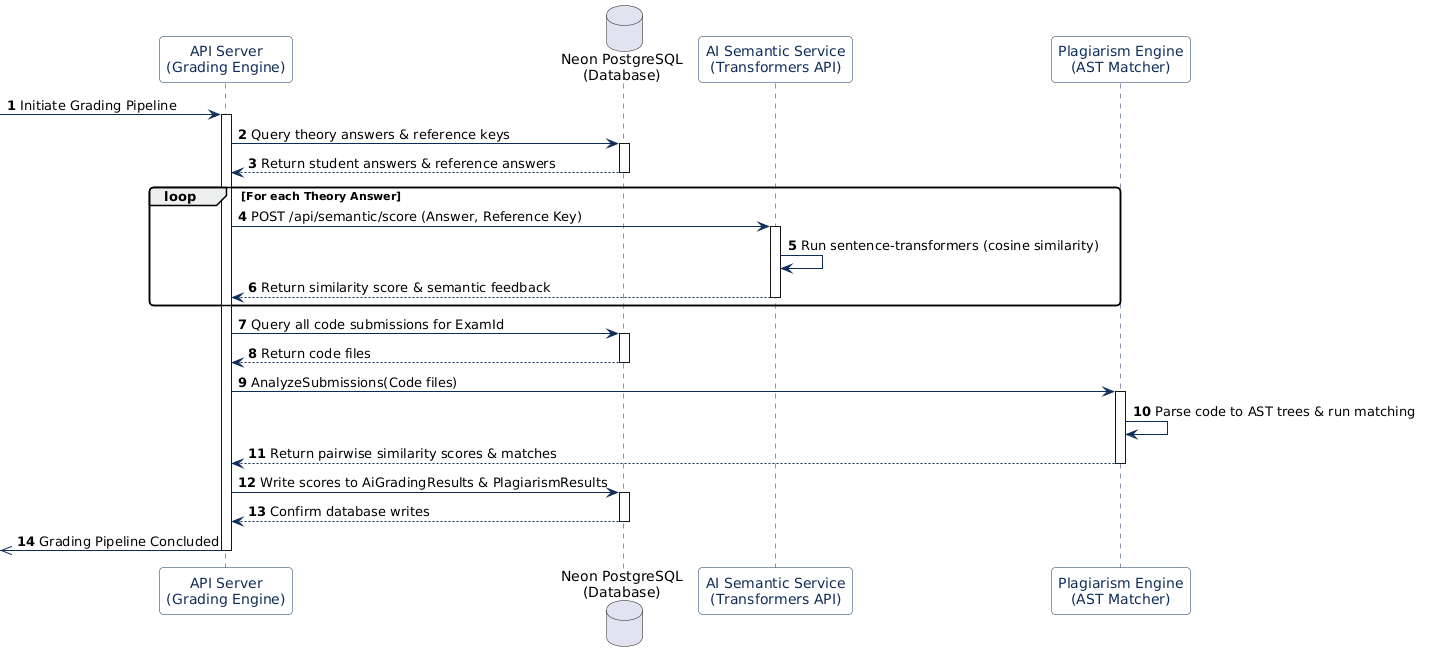
\includegraphics[width=0.75\linewidth,height=367pt,keepaspectratio]{Figures/seq_ai_plagiarism.png}
\caption{Sequence Diagram of Submission, Theory Grading and Plagiarism Check (a): Staging and Theory Grading}
\label{fig:seq_ai_plagiarism}
\end{figure}

\begin{figure}[p]
\centering
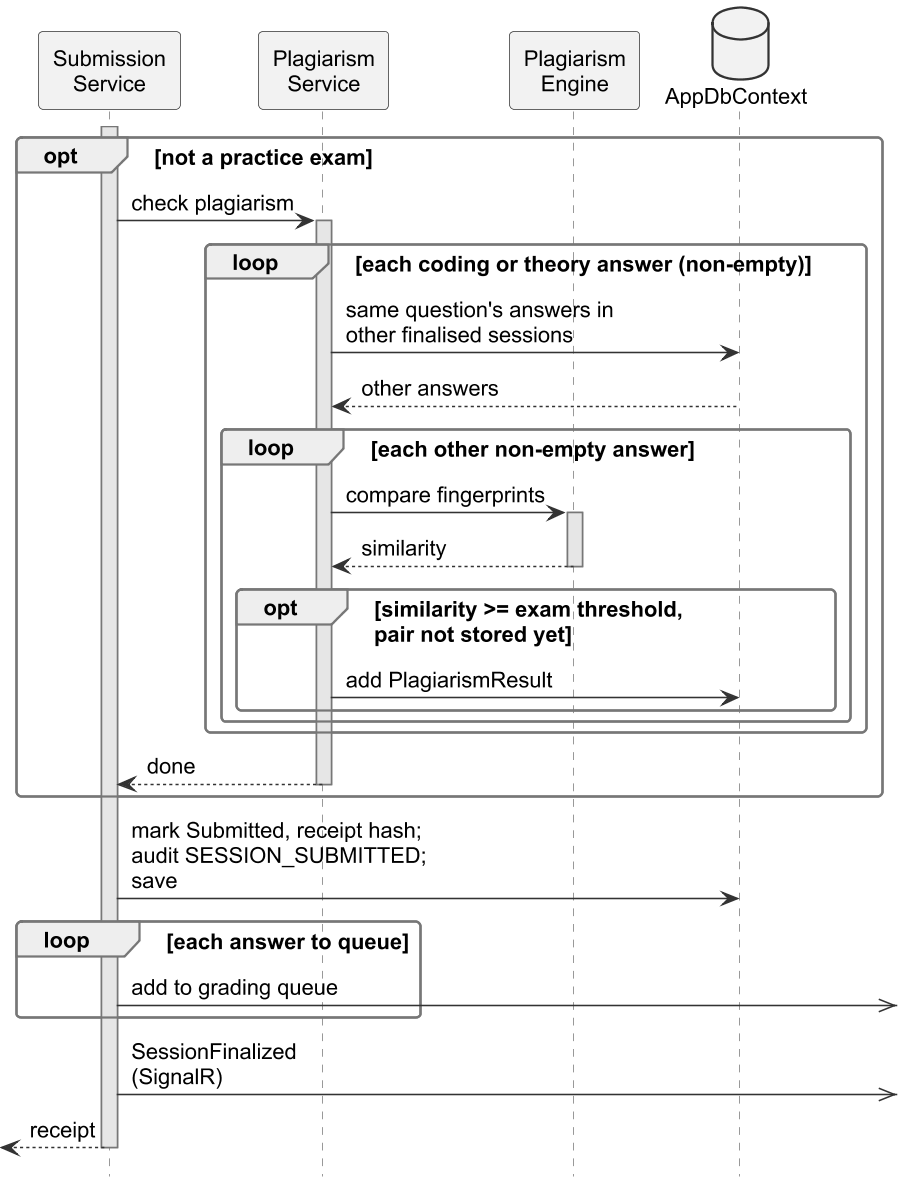
\includegraphics[width=\linewidth,height=470pt,keepaspectratio]{Figures/seq_ai_plagiarism_b.png}
\caption{Sequence Diagram of Submission, Theory Grading and Plagiarism Check (b): Plagiarism Check and Save}
\label{fig:seq_ai_plagiarism_b}
\end{figure}

\begin{sloppypar}
\texttt{GradingWorker} hands each queued answer to \texttt{GradingService}, which picks a runner through \texttt{CodeRunnerResolver} (Docker, else local MinGW), compiles the code once, runs every test case with its time limit and saves the suggested marks in \texttt{AiGradingResults} (Figures~\ref{fig:seq_compilation} and~\ref{fig:seq_compilation_b}).
\end{sloppypar}

\begin{figure}[H]
\centering
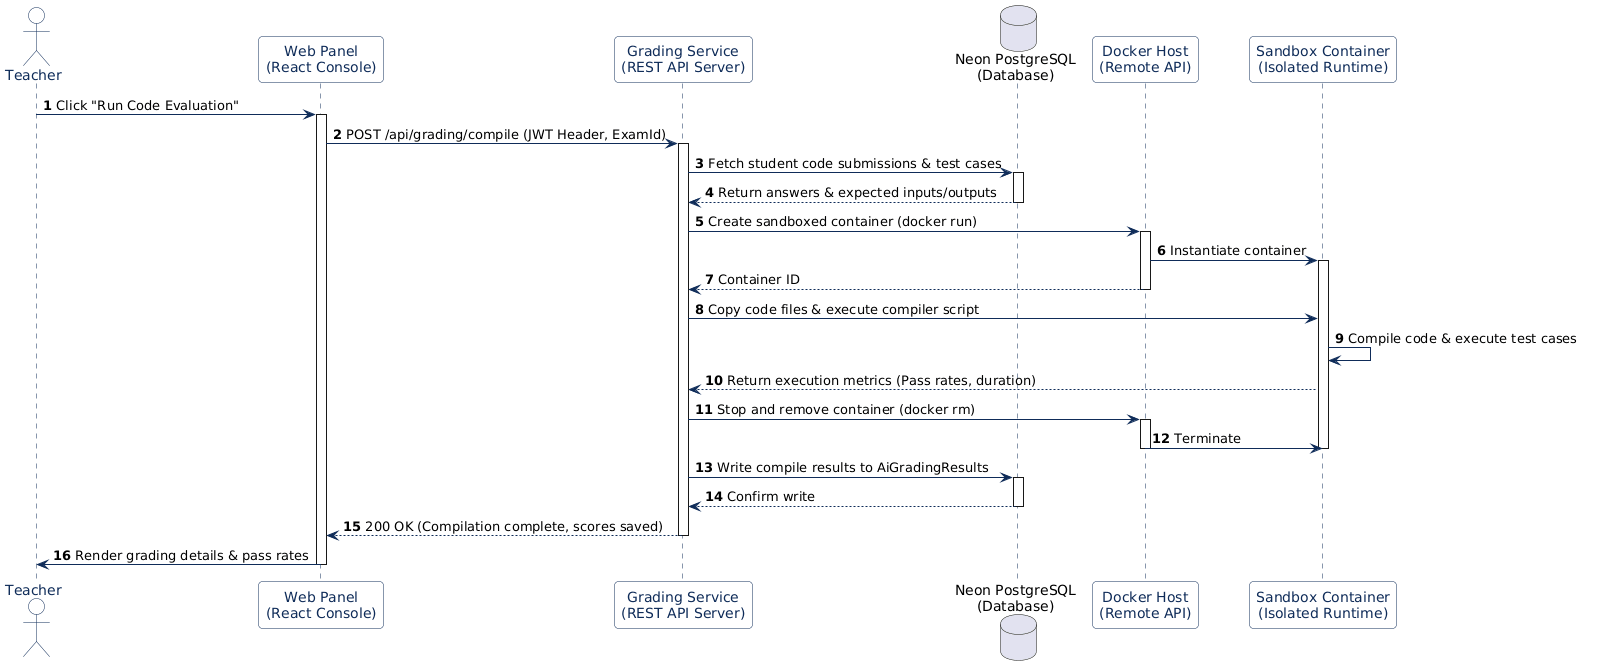
\includegraphics[width=0.90\linewidth,height=253pt,keepaspectratio]{Figures/seq_compilation.png}
\caption{Sequence Diagram of Sandboxed Code Execution (a): Dequeue and Runner Choice}
\label{fig:seq_compilation}
\end{figure}

\begin{figure}[p]
\centering
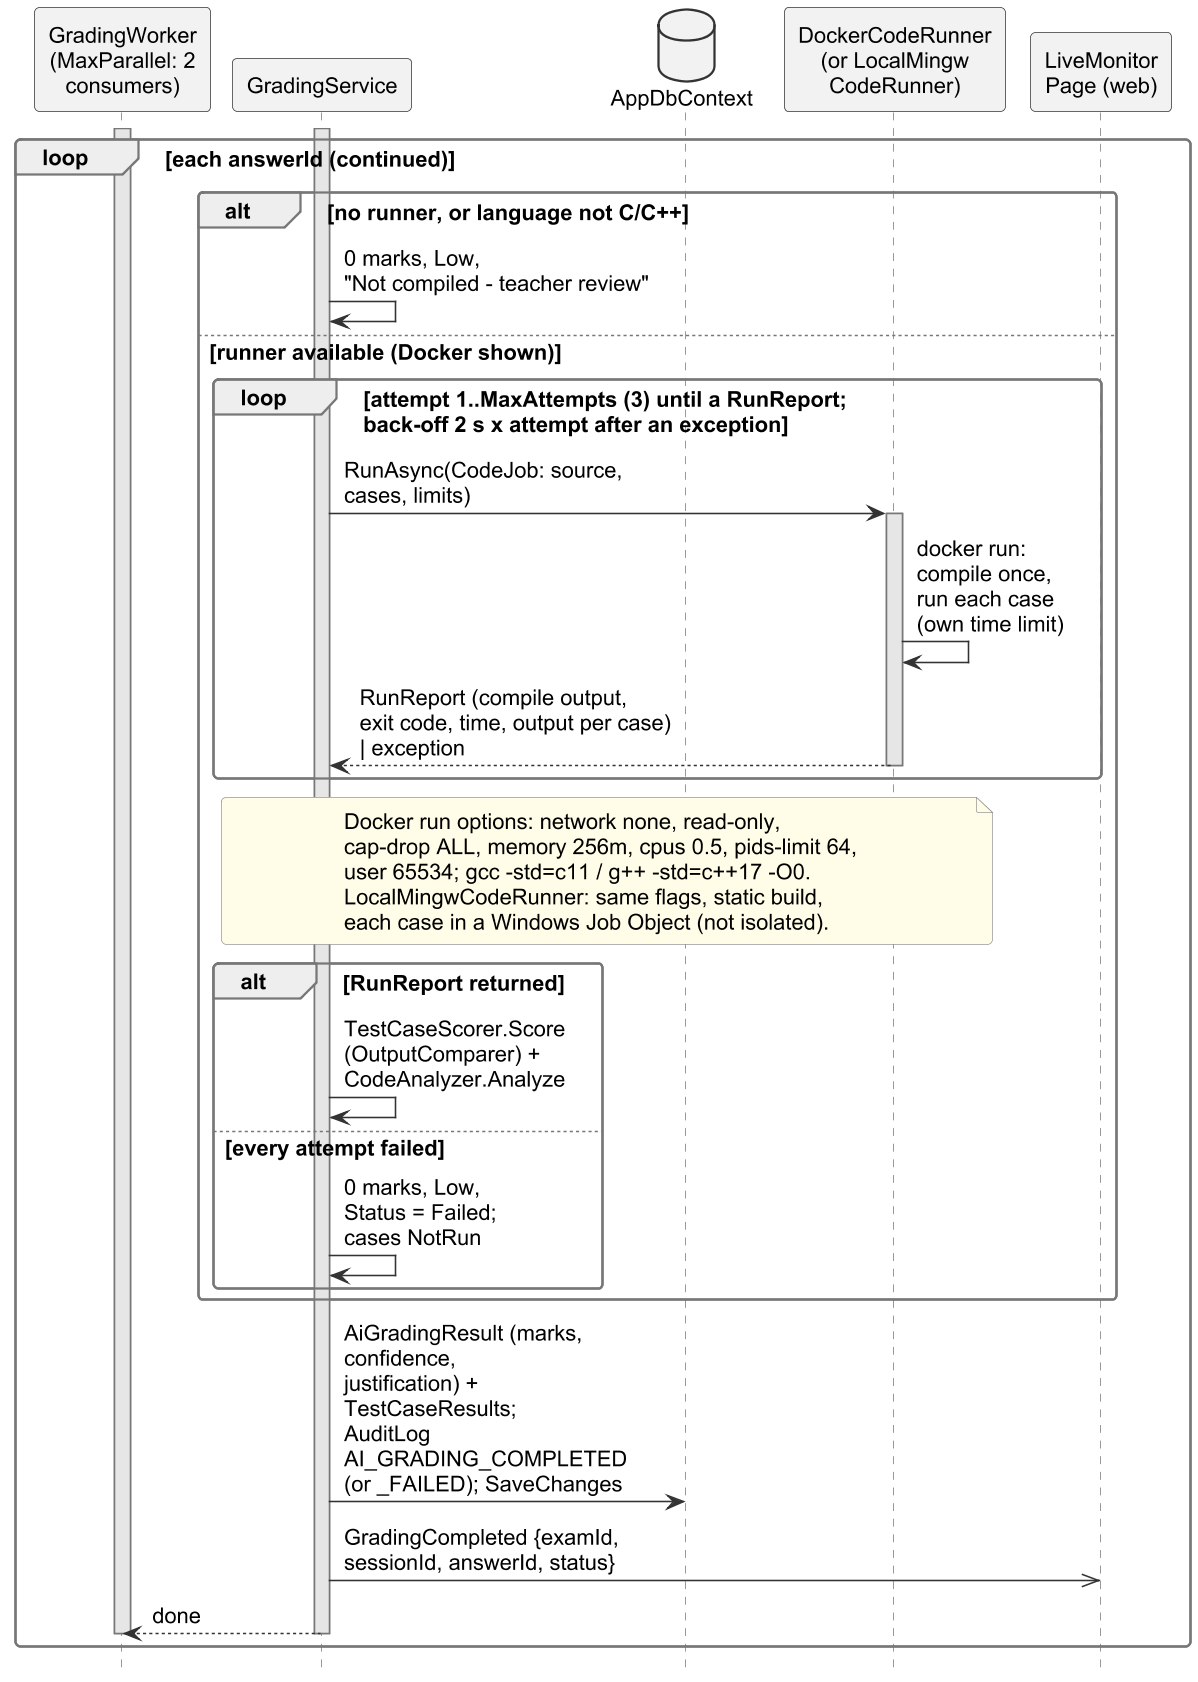
\includegraphics[width=0.90\linewidth,height=570pt,keepaspectratio]{Figures/seq_compilation_b.png}
\caption{Sequence Diagram of Sandboxed Code Execution (b): Compile, Run and Score}
\label{fig:seq_compilation_b}
\end{figure}

\DiagramBarrier
\subsubsection{Readiness Checks, Practice Exam, Lockdown and Recovery (M2, M4, M6; UC-02, UC-03, UC-06, UC-08)}
\begin{sloppypar}
In Figures~\ref{fig:seq_diagnostics} and~\ref{fig:seq_diagnostics_b} the client runs the seven readiness checks and posts the result; the server re-checks it, stores a \texttt{ReadinessCheck} row with its audit entry and returns a pass valid for 30 minutes.
\end{sloppypar}

\begin{figure}[H]
\centering
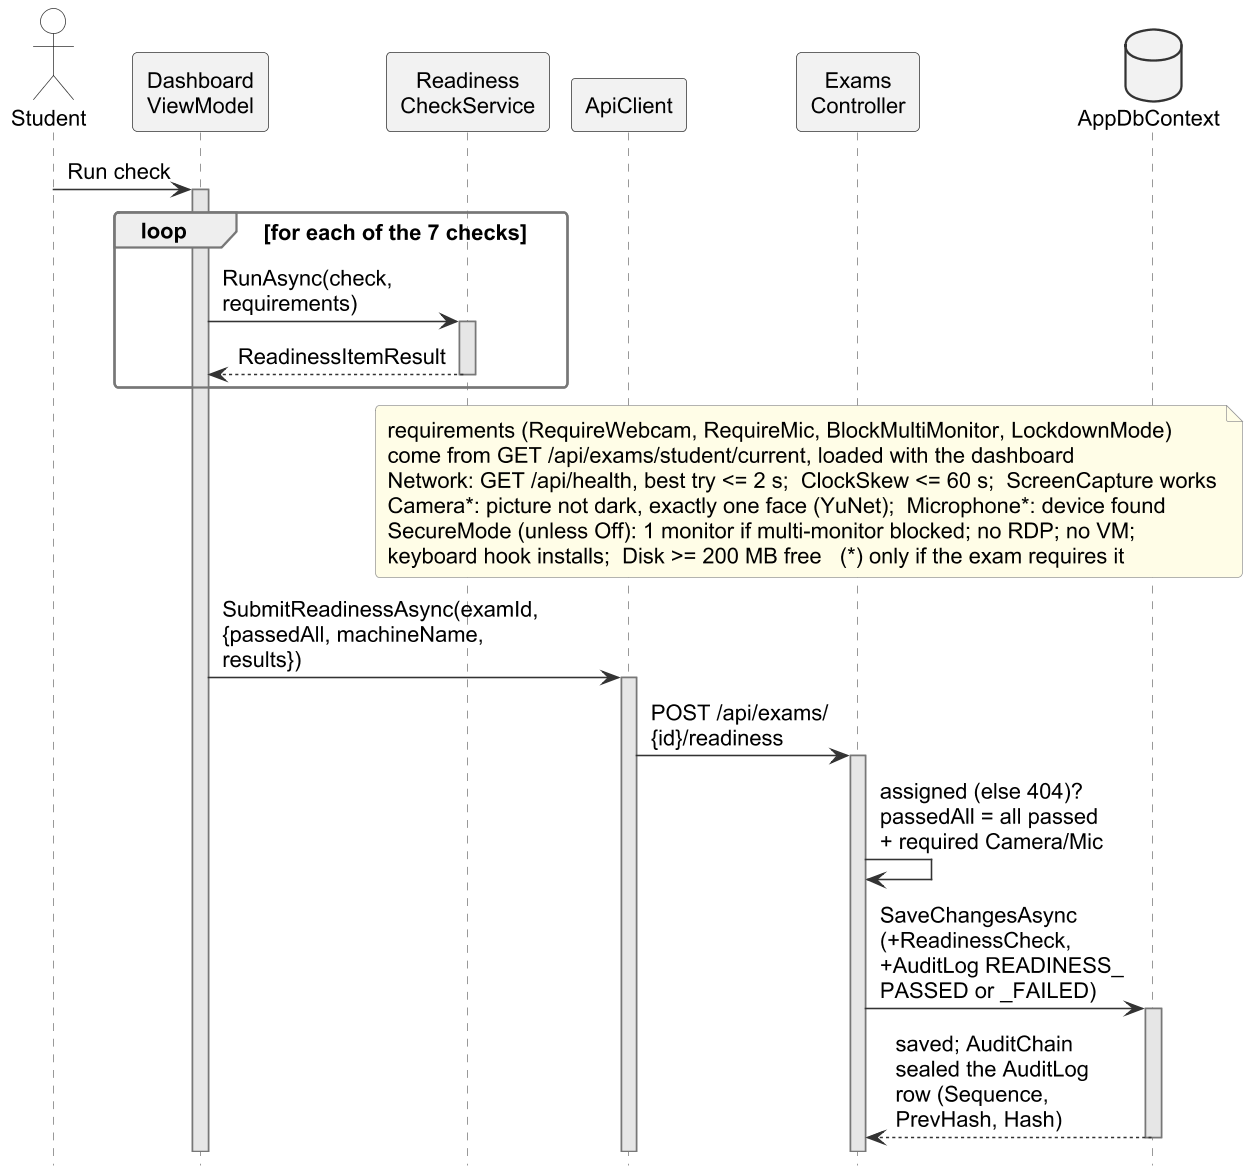
\includegraphics[width=\linewidth,height=423pt,keepaspectratio]{Figures/seq_diagnostics.png}
\caption{Sequence Diagram of Pre-Exam Readiness Checks (a): Running and Posting the Checks}
\label{fig:seq_diagnostics}
\end{figure}

\begin{figure}[H]
\centering
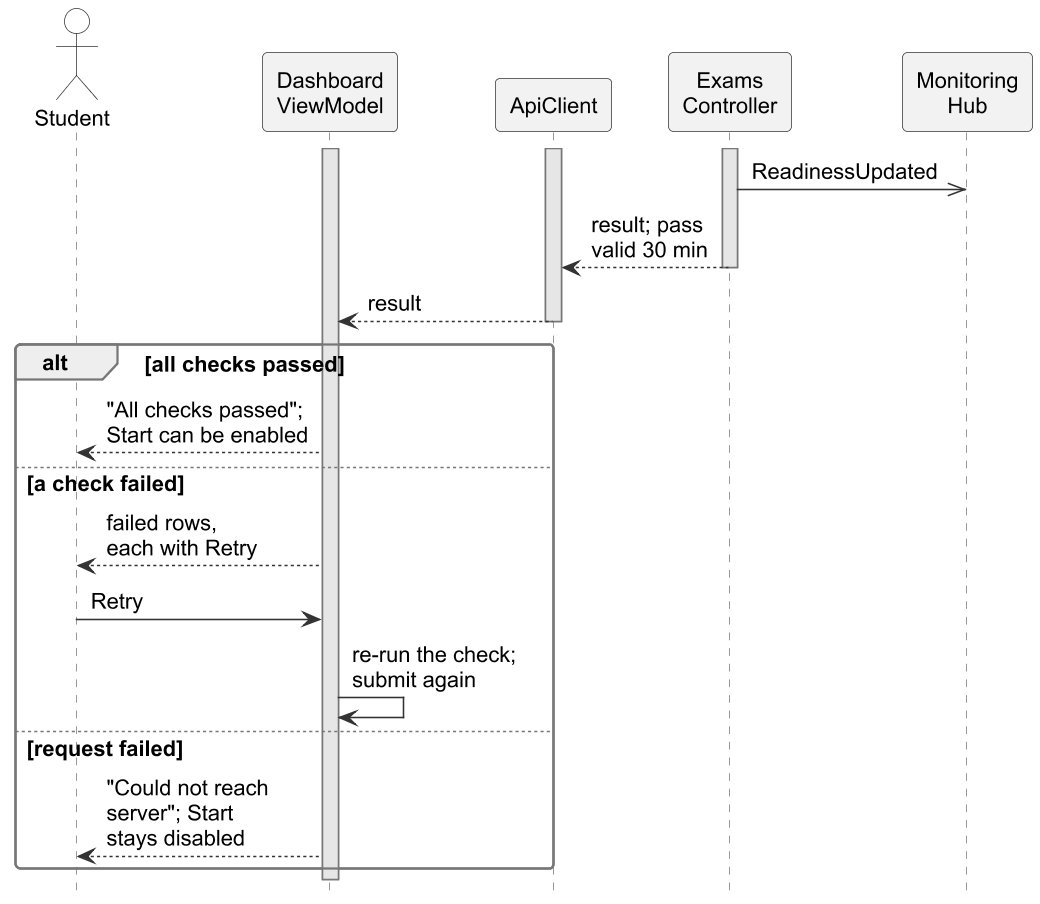
\includegraphics[width=\linewidth,height=410pt,keepaspectratio]{Figures/seq_diagnostics_b.png}
\caption{Sequence Diagram of Pre-Exam Readiness Checks (b): Live Update and Result}
\label{fig:seq_diagnostics_b}
\end{figure}

\begin{sloppypar}
A practice exam is listed by \texttt{GET} \url{/api/exams/student/practice} and started with \texttt{POST} \url{/api/exams/{id}/start-session} (a real exam uses \url{/api/exams/student/start}); it then uses the same save and submit calls, in Report mode without the webcam (Figures~\ref{fig:seq_readiness} to~\ref{fig:seq_readiness_c}).
\end{sloppypar}

\begin{figure}[H]
\centering
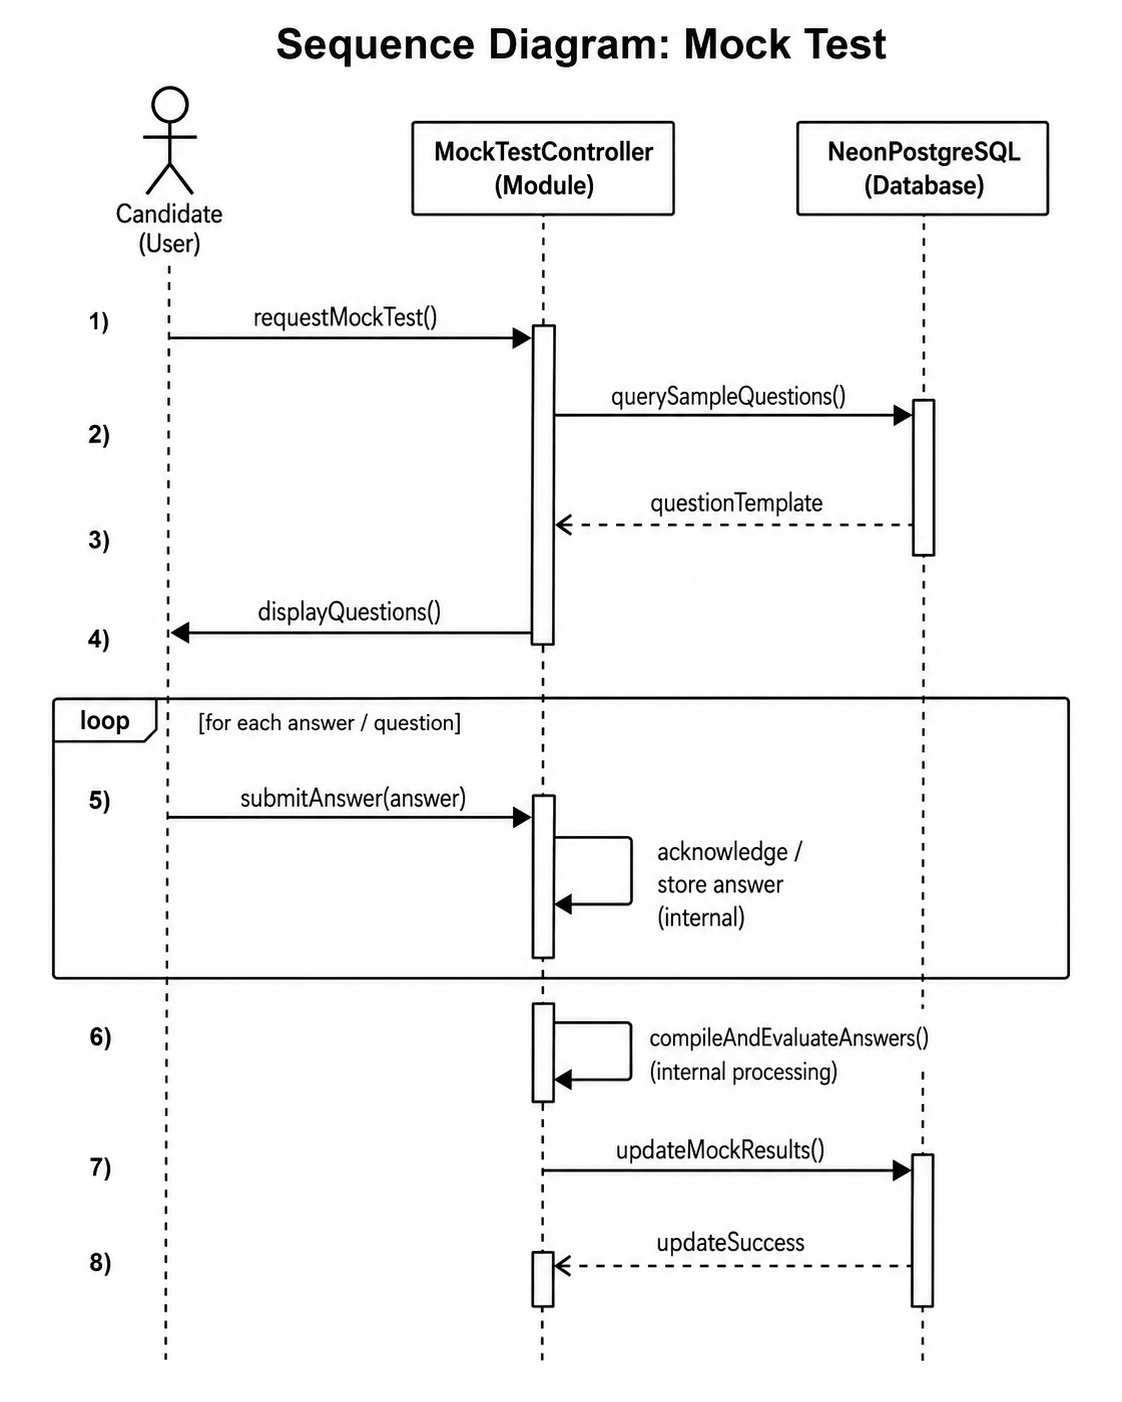
\includegraphics[width=0.85\linewidth,height=207pt,keepaspectratio]{Figures/seq_readiness.png}
\caption{Sequence Diagram of the Practice Exam (a): Practice List}
\label{fig:seq_readiness}
\end{figure}

\begin{figure}[H]
\centering
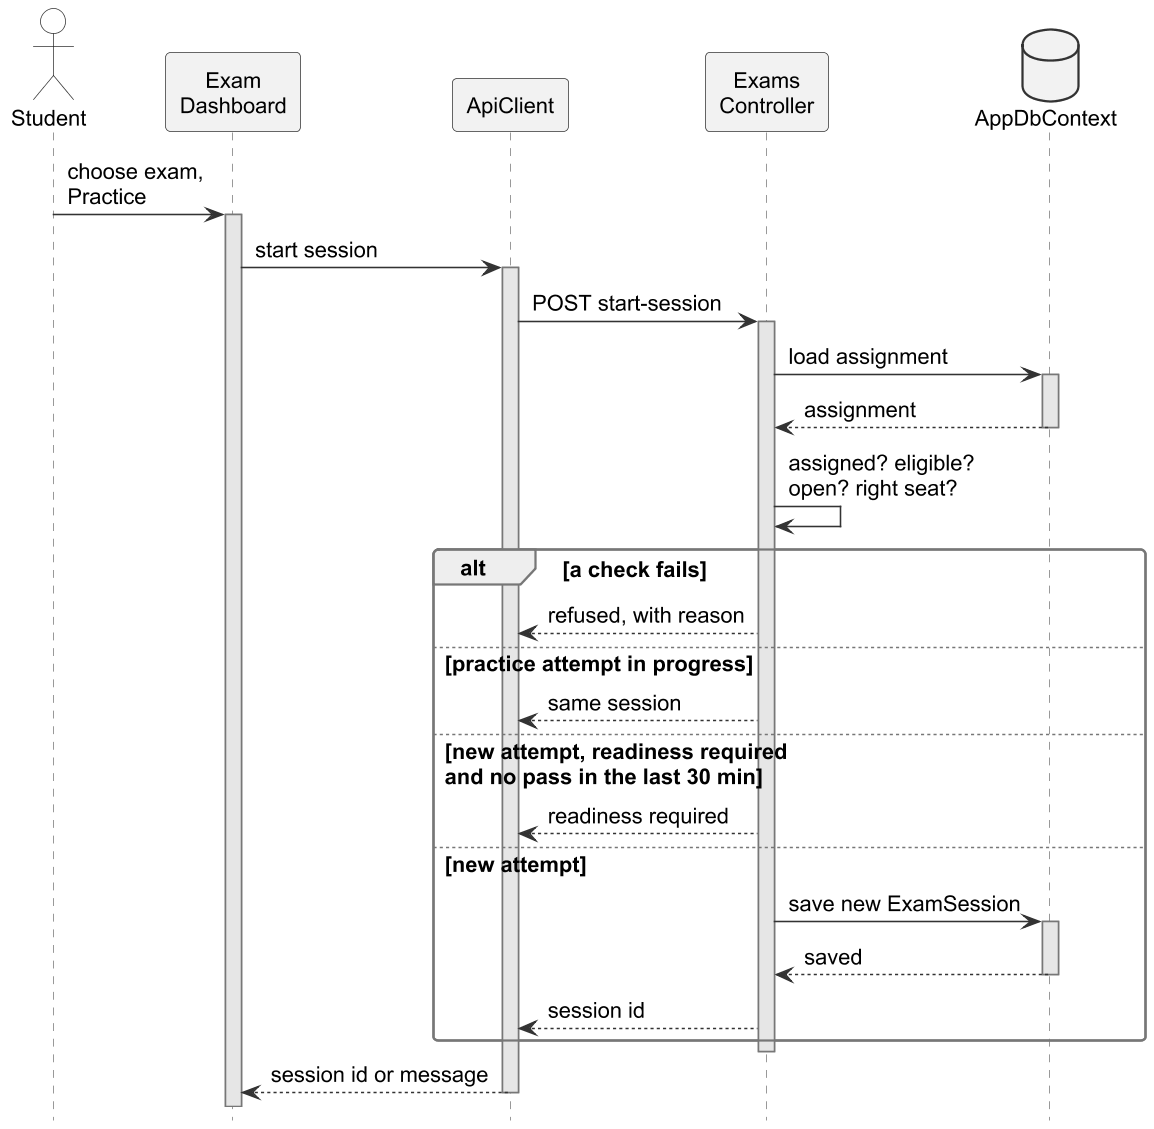
\includegraphics[width=0.90\linewidth,height=395pt,keepaspectratio]{Figures/seq_readiness_b.png}
\caption{Sequence Diagram of the Practice Exam (b): Start-Session Gates}
\label{fig:seq_readiness_b}
\end{figure}

\begin{figure}[H]
\centering
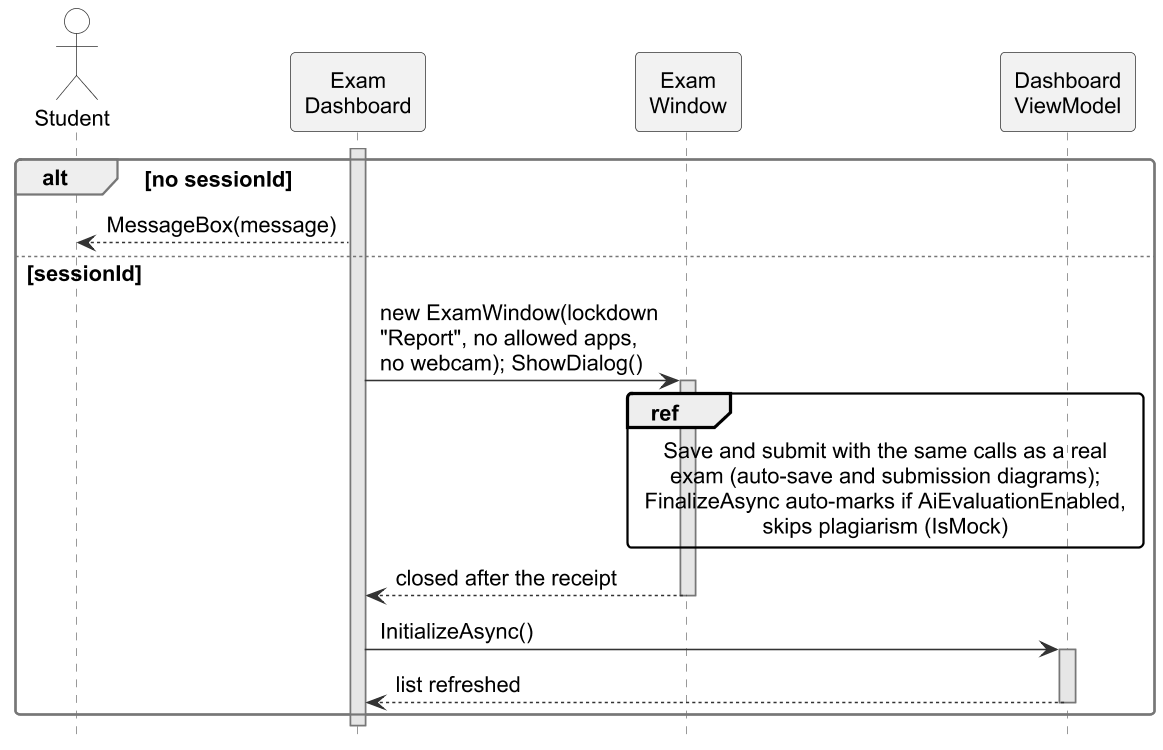
\includegraphics[width=0.90\linewidth,height=262pt,keepaspectratio]{Figures/seq_readiness_c.png}
\caption{Sequence Diagram of the Practice Exam (c): Practice Window}
\label{fig:seq_readiness_c}
\end{figure}

At exam start the \texttt{LockdownCoordinator} installs a low-level keyboard hook that blocks Alt+Tab, the Windows keys and similar shortcuts, disables Task Manager through the registry and starts the clipboard, process and device guards. Violations pass a 15-second cooldown and go to the encrypted monitoring outbox (Figures~\ref{fig:seq_lockdown} to~\ref{fig:seq_lockdown_c}).

\begin{figure}[H]
\centering
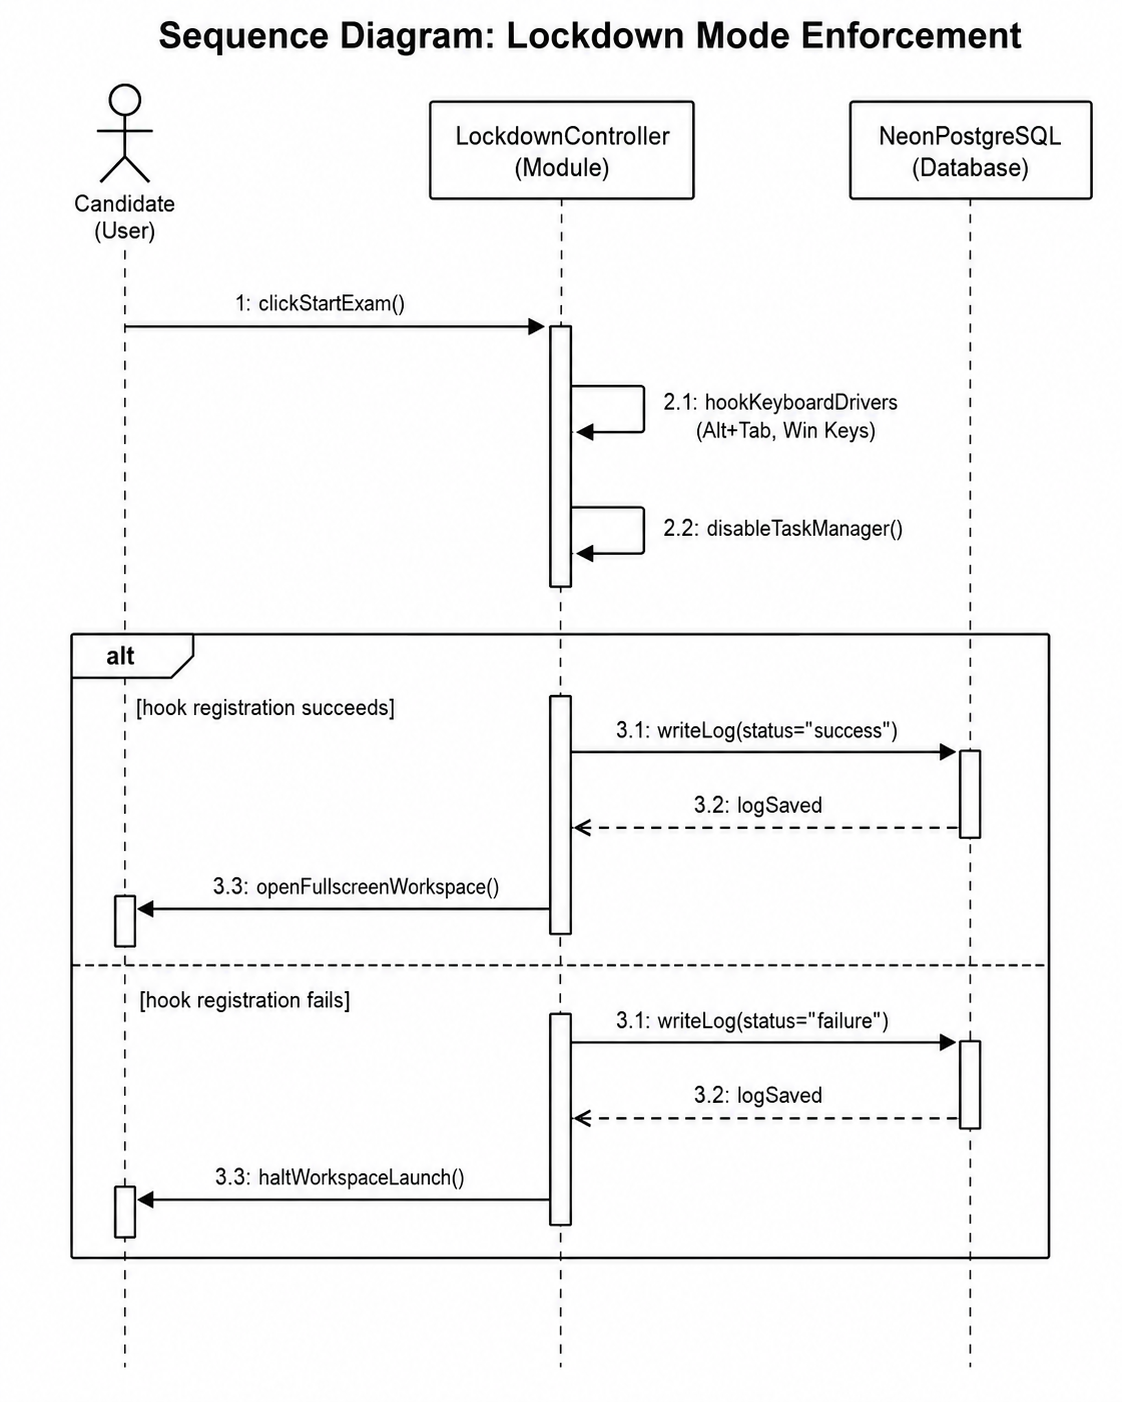
\includegraphics[width=0.90\linewidth,height=534pt,keepaspectratio]{Figures/seq_lockdown.png}
\caption{Sequence Diagram of Lockdown Enforcement (a): Start and Guard Events}
\label{fig:seq_lockdown}
\end{figure}

\begin{figure}[H]
\centering
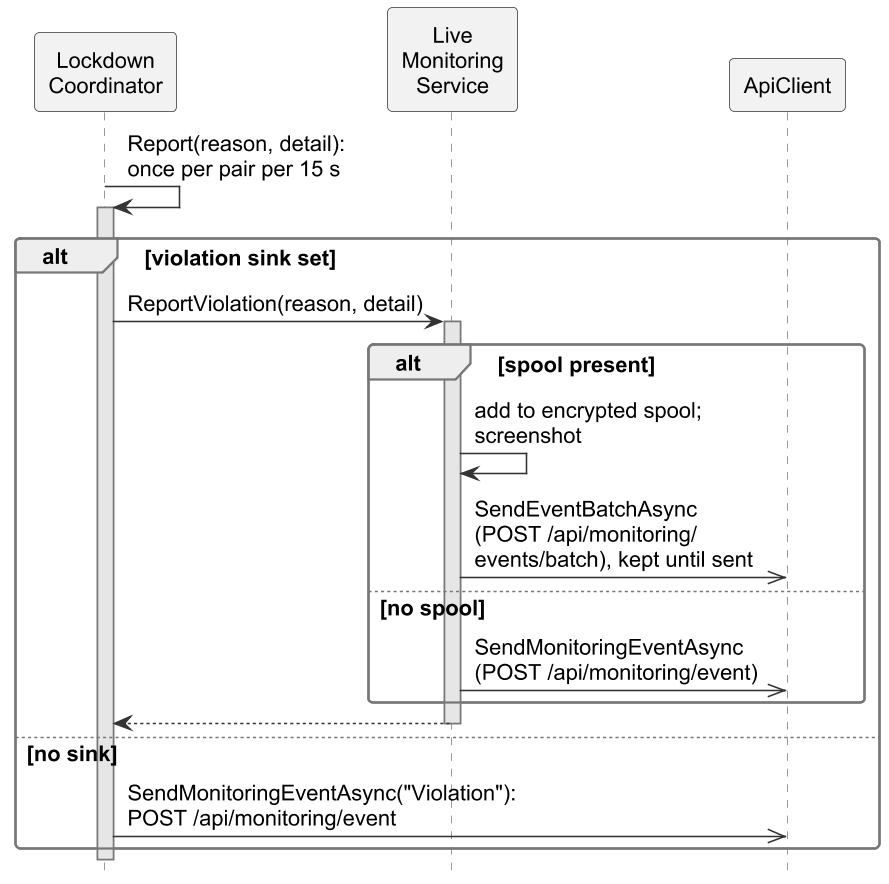
\includegraphics[width=0.65\linewidth,height=292pt,keepaspectratio]{Figures/seq_lockdown_b.png}
\caption{Sequence Diagram of Lockdown Enforcement (b): Violation Reporting}
\label{fig:seq_lockdown_b}
\end{figure}

\begin{figure}[H]
\centering
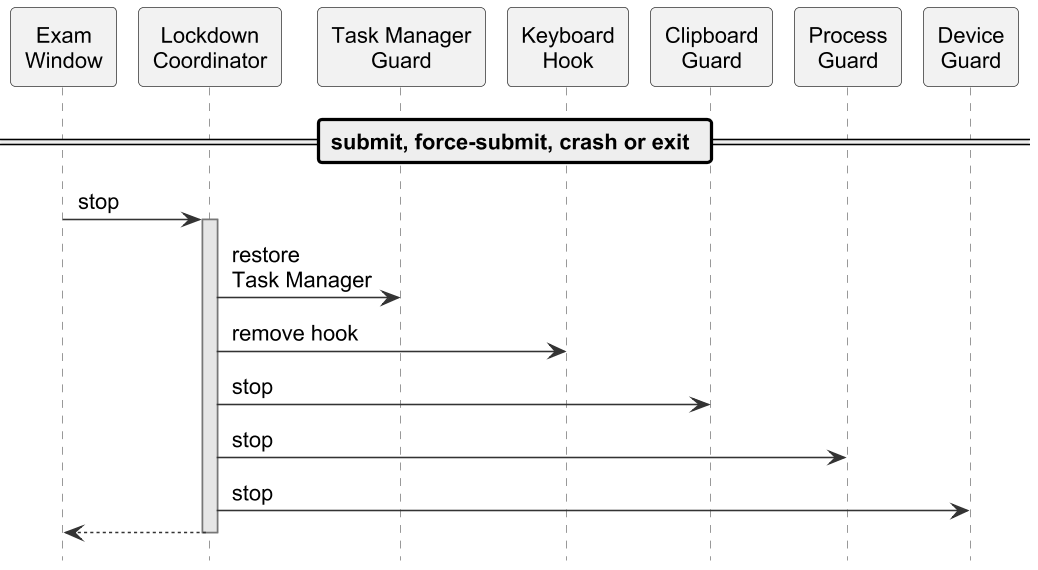
\includegraphics[width=0.85\linewidth,height=211pt,keepaspectratio]{Figures/seq_lockdown_c.png}
\caption{Sequence Diagram of Lockdown Enforcement (c): Release}
\label{fig:seq_lockdown_c}
\end{figure}

Figures~\ref{fig:seq_recovery} and~\ref{fig:seq_recovery_b} show the save, offline queue, backup and replay calls; after a crash the backup is merged by revision, or ignored if it was tampered with.

\begin{figure}[H]
\centering
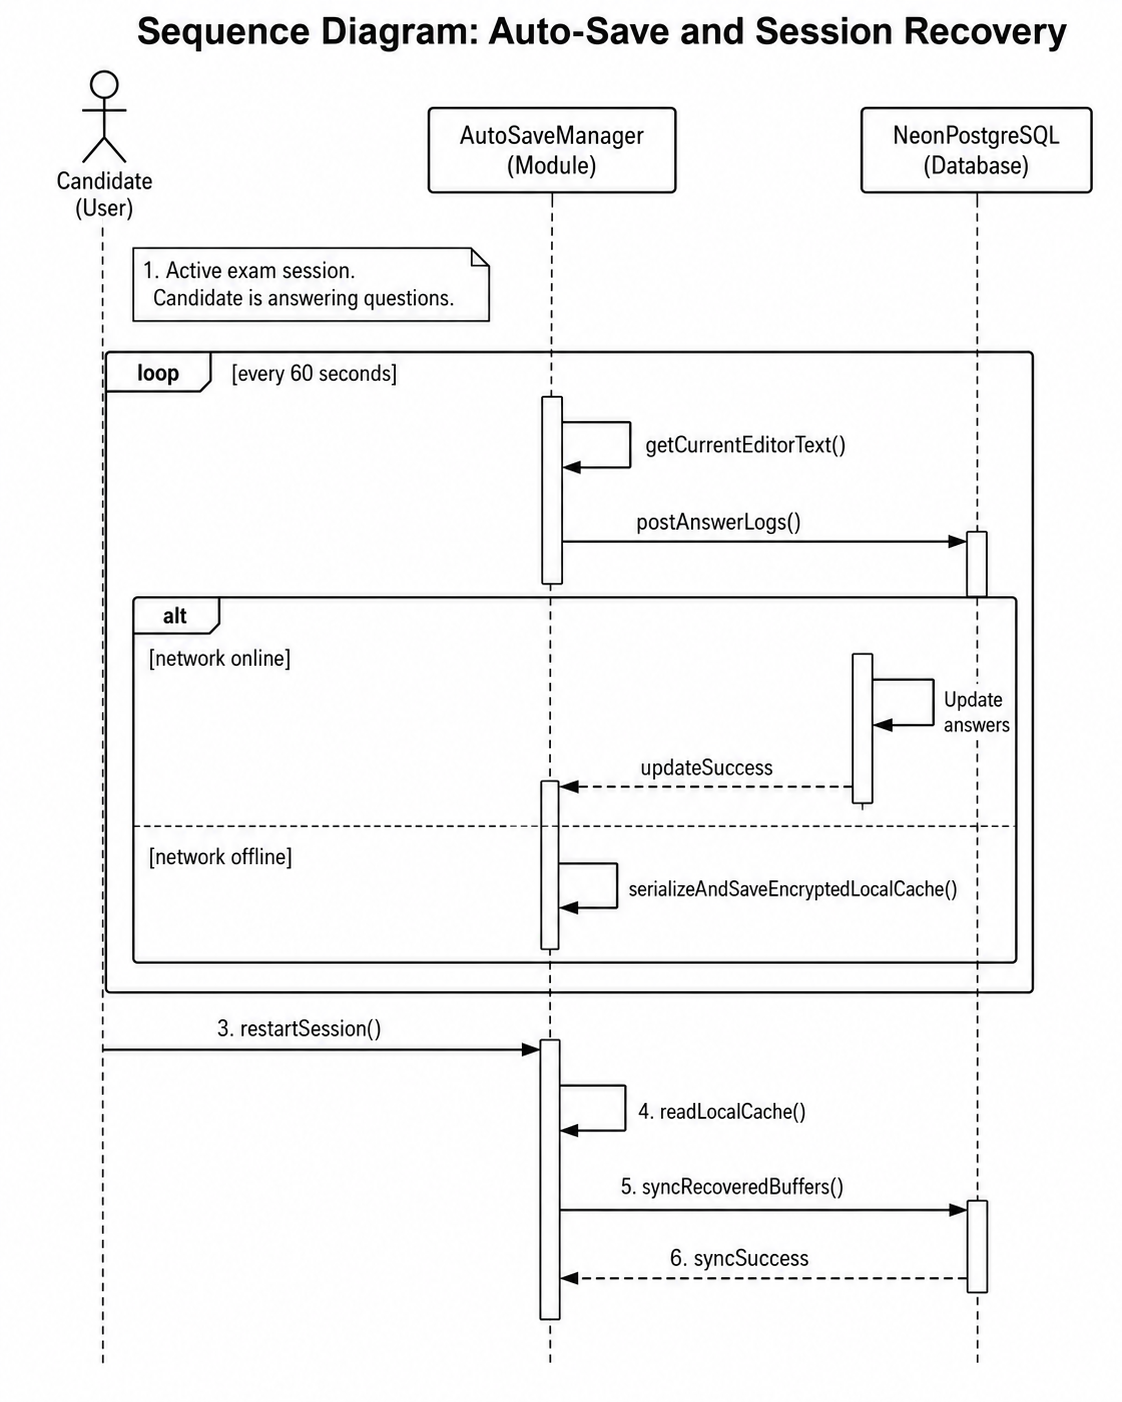
\includegraphics[width=\linewidth,height=464pt,keepaspectratio]{Figures/seq_recovery.png}
\caption{Sequence Diagram of Autosave and Recovery (a): Autosave and Offline Queue}
\label{fig:seq_recovery}
\end{figure}

\begin{figure}[H]
\centering
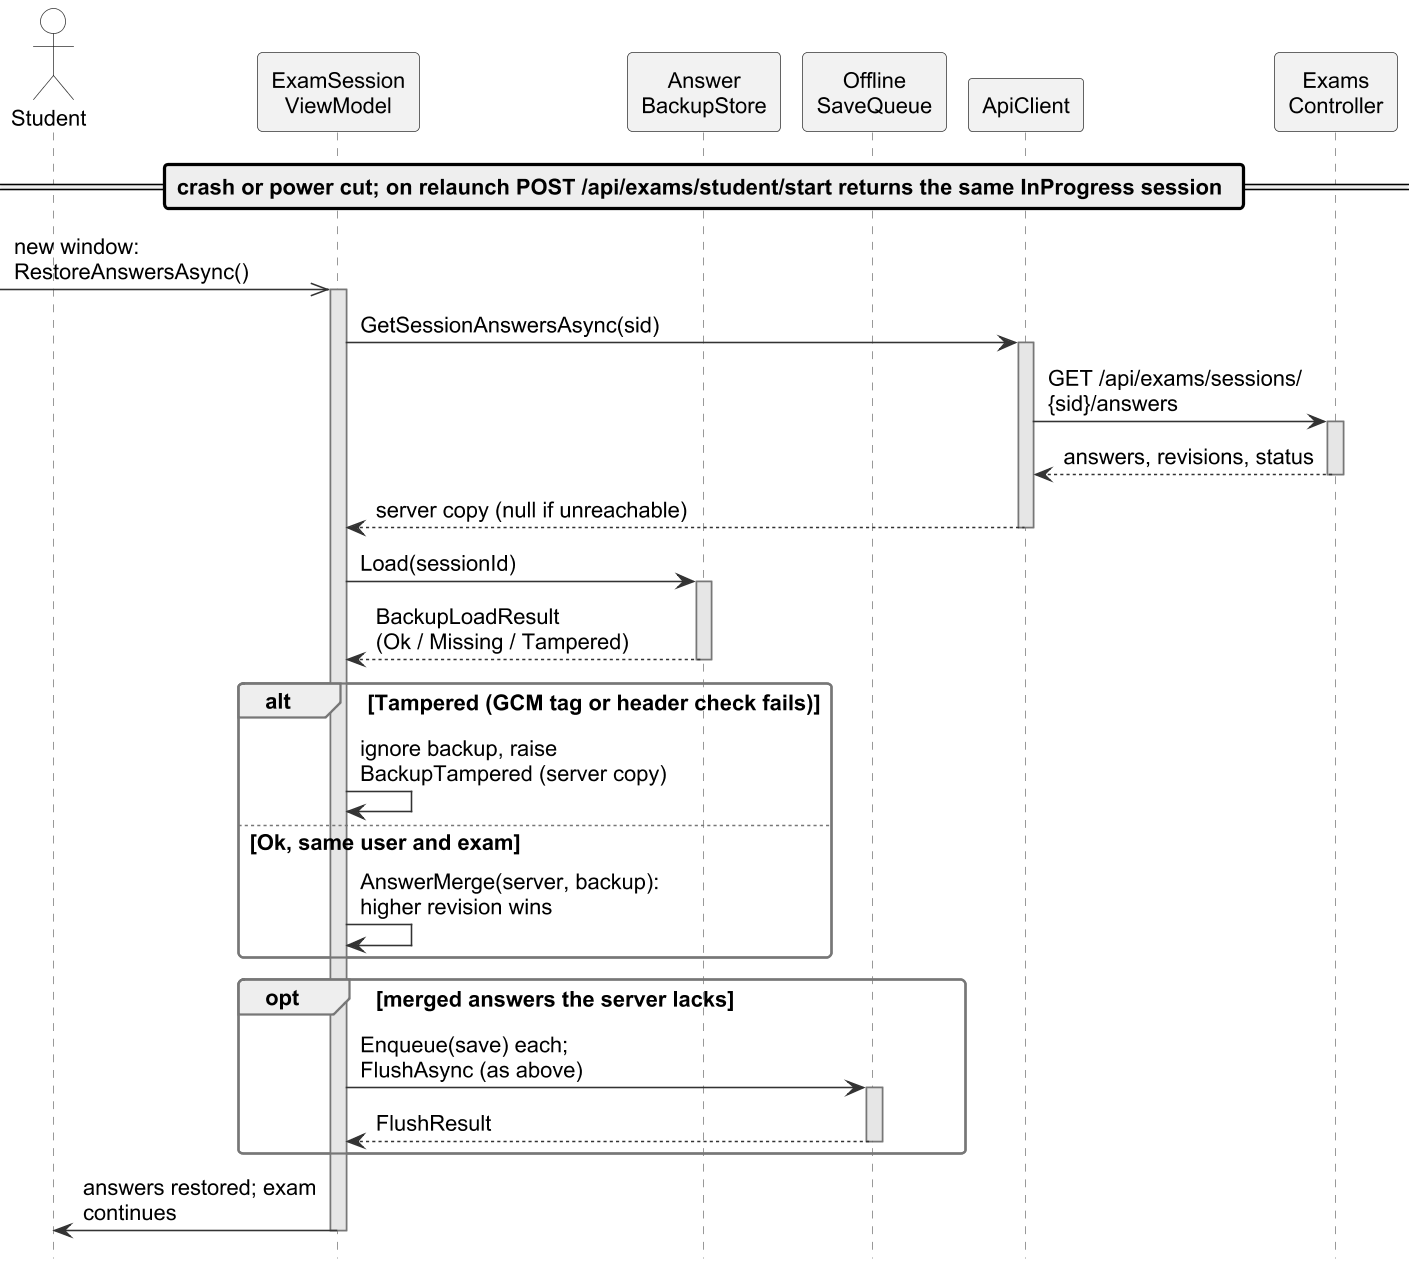
\includegraphics[width=\linewidth,height=404pt,keepaspectratio]{Figures/seq_recovery_b.png}
\caption{Sequence Diagram of Autosave and Recovery (b): Recovery after a Crash}
\label{fig:seq_recovery_b}
\end{figure}

\DiagramBarrier
\subsubsection{Submission, Configuration and Report Export (M6, M8, M12; UC-08, UC-13, UC-18, UC-21)}
\begin{sloppypar}
On submit (Figures~\ref{fig:seq_submission} to~\ref{fig:seq_submission_c}) the client first flushes unsent saves; while one is still offline the window stays open. The server checks that the session is the caller's own and in progress, then in one save sets it to Submitted with the receipt hash and stores the staged grades, the plagiarism pairs and the \texttt{SESSION\_SUBMITTED} audit entry; it then queues the coding answers. The client verifies the receipt and releases the lockdown.
\end{sloppypar}

\begin{figure}[H]
\centering
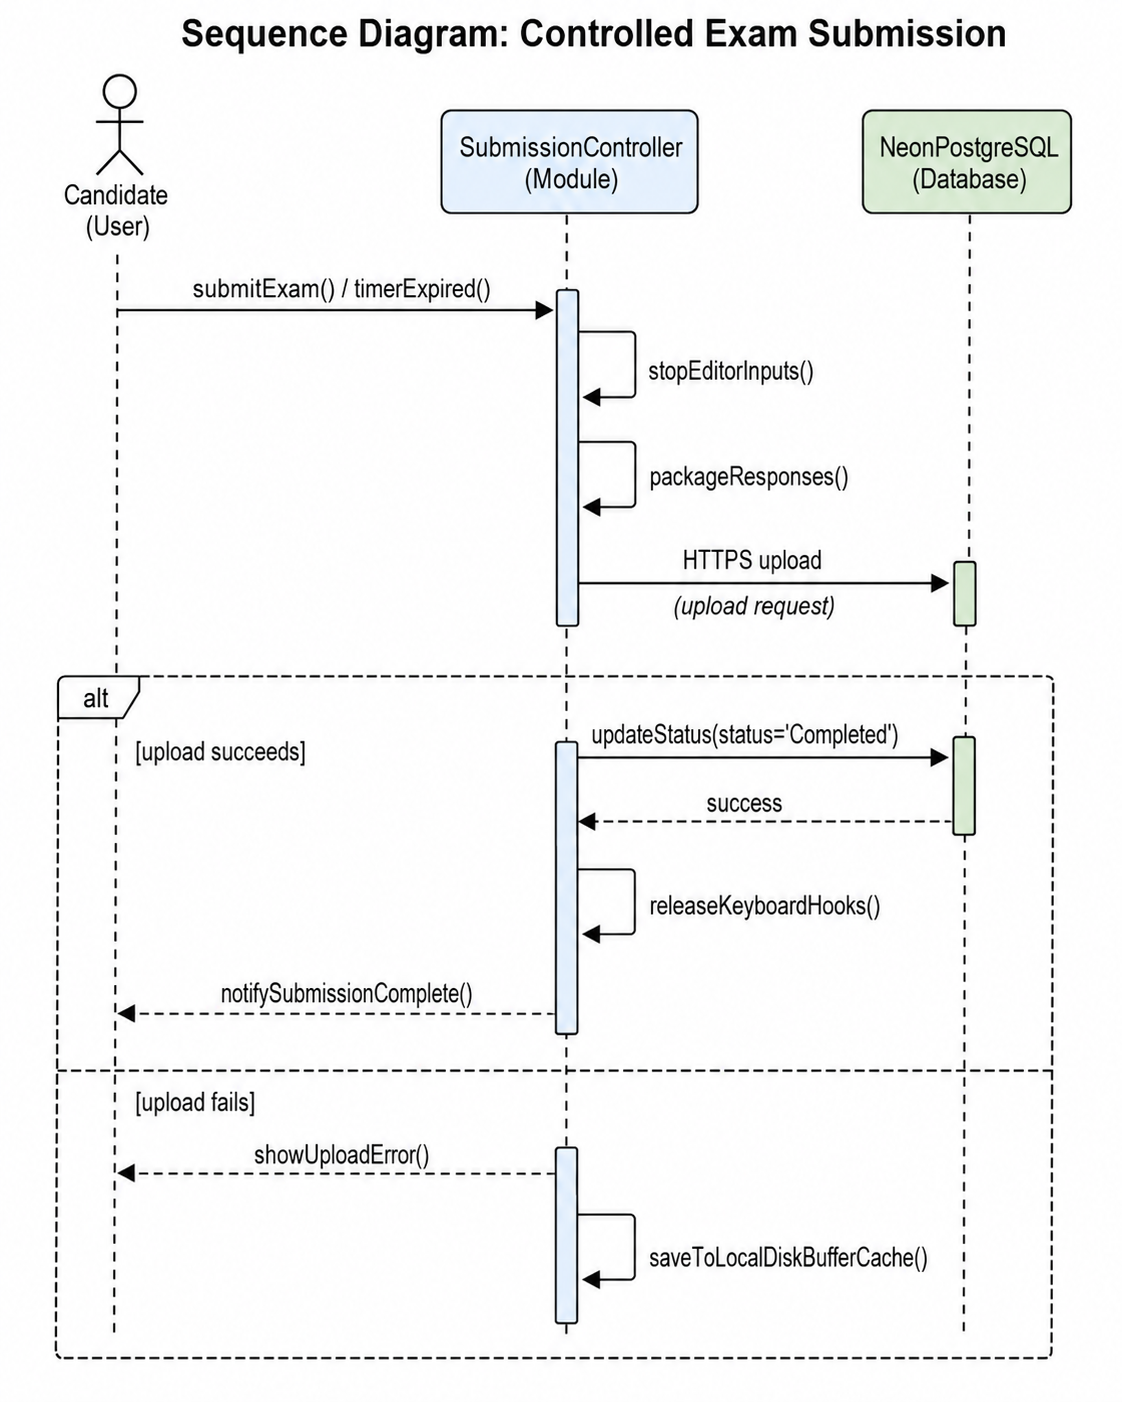
\includegraphics[width=0.95\linewidth,height=385pt,keepaspectratio]{Figures/seq_submission.png}
\caption{Sequence Diagram of Exam Submission (a): Flush and Submit Request}
\label{fig:seq_submission}
\end{figure}

\begin{figure}[H]
\centering
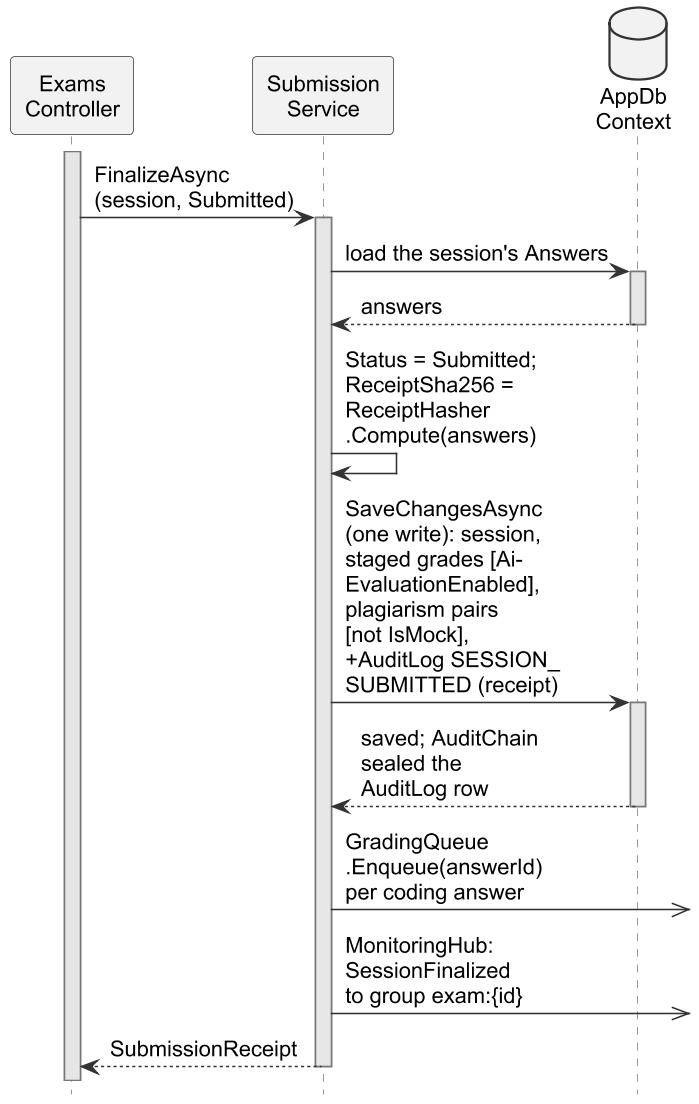
\includegraphics[width=0.55\linewidth,height=392pt,keepaspectratio]{Figures/seq_submission_b.png}
\caption{Sequence Diagram of Exam Submission (b): Finalisation}
\label{fig:seq_submission_b}
\end{figure}

\begin{figure}[H]
\centering
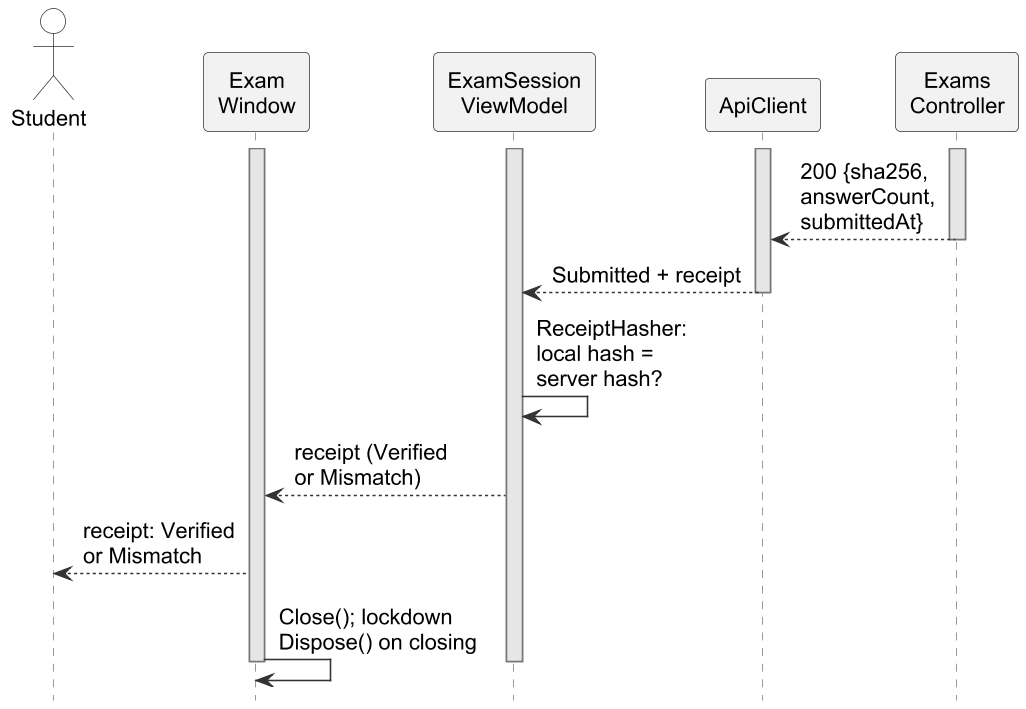
\includegraphics[width=0.80\linewidth,height=249pt,keepaspectratio]{Figures/seq_submission_c.png}
\caption{Sequence Diagram of Exam Submission (c): Receipt Check}
\label{fig:seq_submission_c}
\end{figure}

Exam configuration (Figure~\ref{fig:seq_config}) loads the teacher's sections and students, then makes one create or update call to \texttt{ExamsController} carrying the questions and test cases.

\begin{figure}[p]
\centering
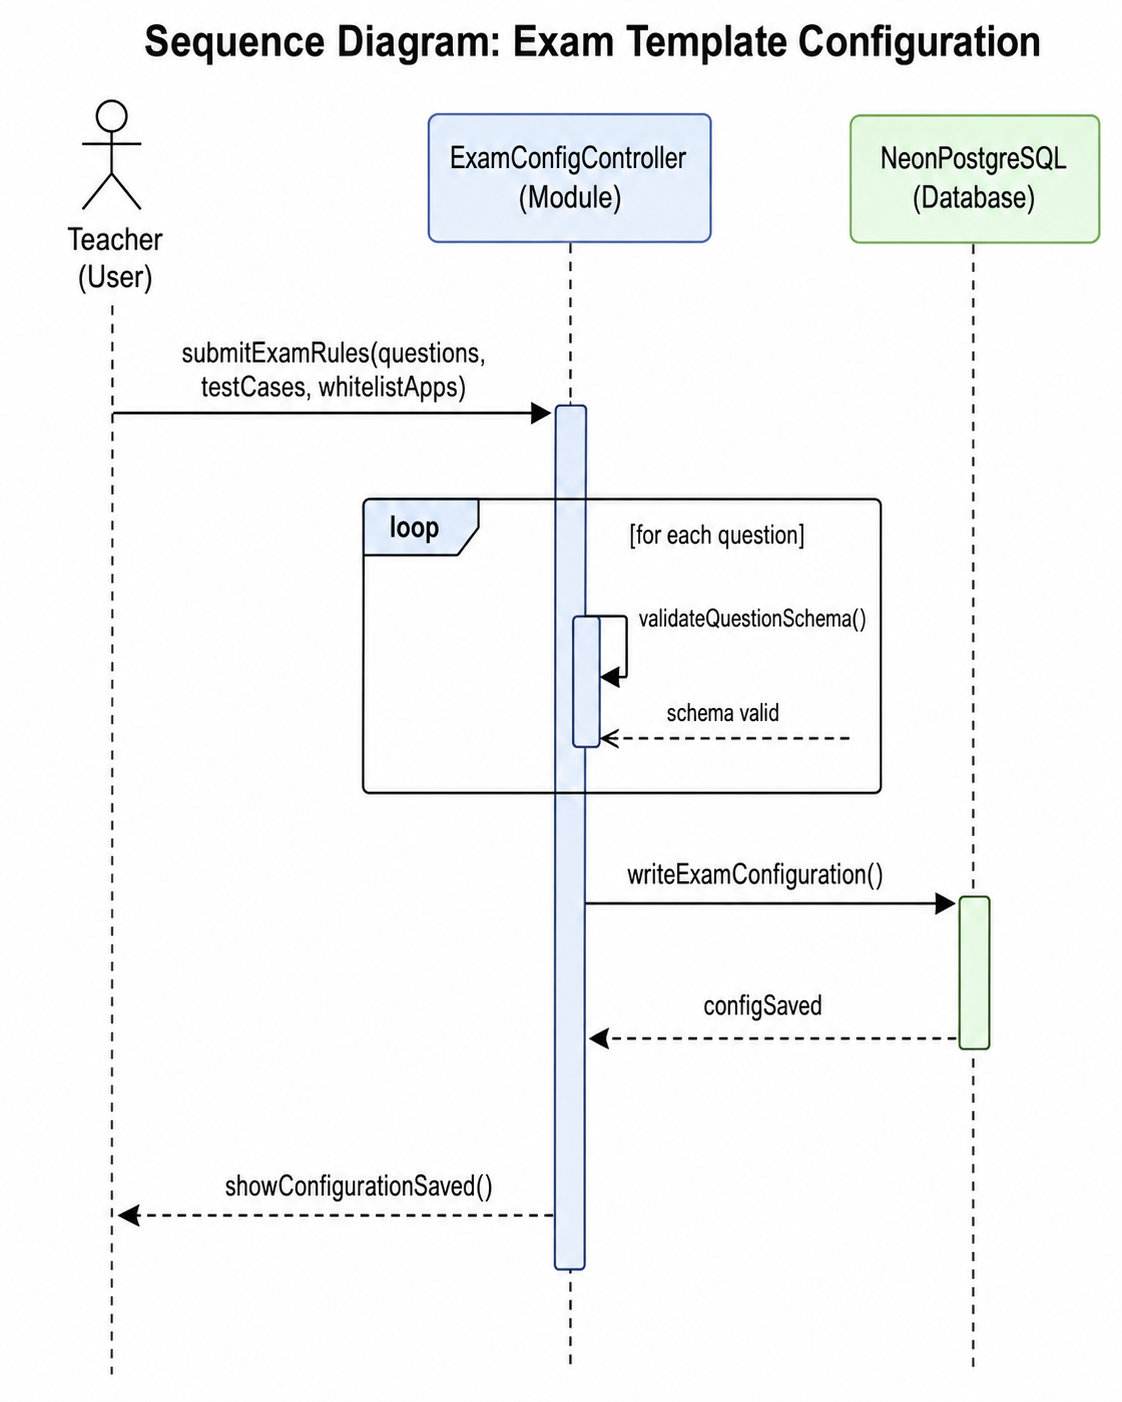
\includegraphics[width=0.90\linewidth,height=628pt,keepaspectratio]{Figures/seq_config.png}
\caption{Sequence Diagram of Exam Configuration}
\label{fig:seq_config}
\end{figure}

\begin{sloppypar}
For an export (Figures~\ref{fig:seq_audit} and~\ref{fig:seq_audit_b}) \texttt{AnalyticsController} checks the report type and that the caller owns the exam or is an admin. \texttt{ReportExportService} writes the PDF, Excel file or ZIP to \texttt{Reports/} and, in one \texttt{SaveChanges}, adds an \texttt{ExamReport} row and a \texttt{REPORT\_GENERATED} audit entry with the file's type, name, SHA-256 and size. The download re-checks the bare file name, the \texttt{ExamReport} row, ownership and that the file exists. An admin verifies the chain with \texttt{GET} \url{/api/audit-logs/verify}, which recomputes every hash and reports a valid chain, the first broken row, or unsealed rows. The exam summary PDF (\texttt{POST} \url{/api/analytics/exams/{id}/report}) writes no audit entry.
\end{sloppypar}

\begin{figure}[p]
\centering
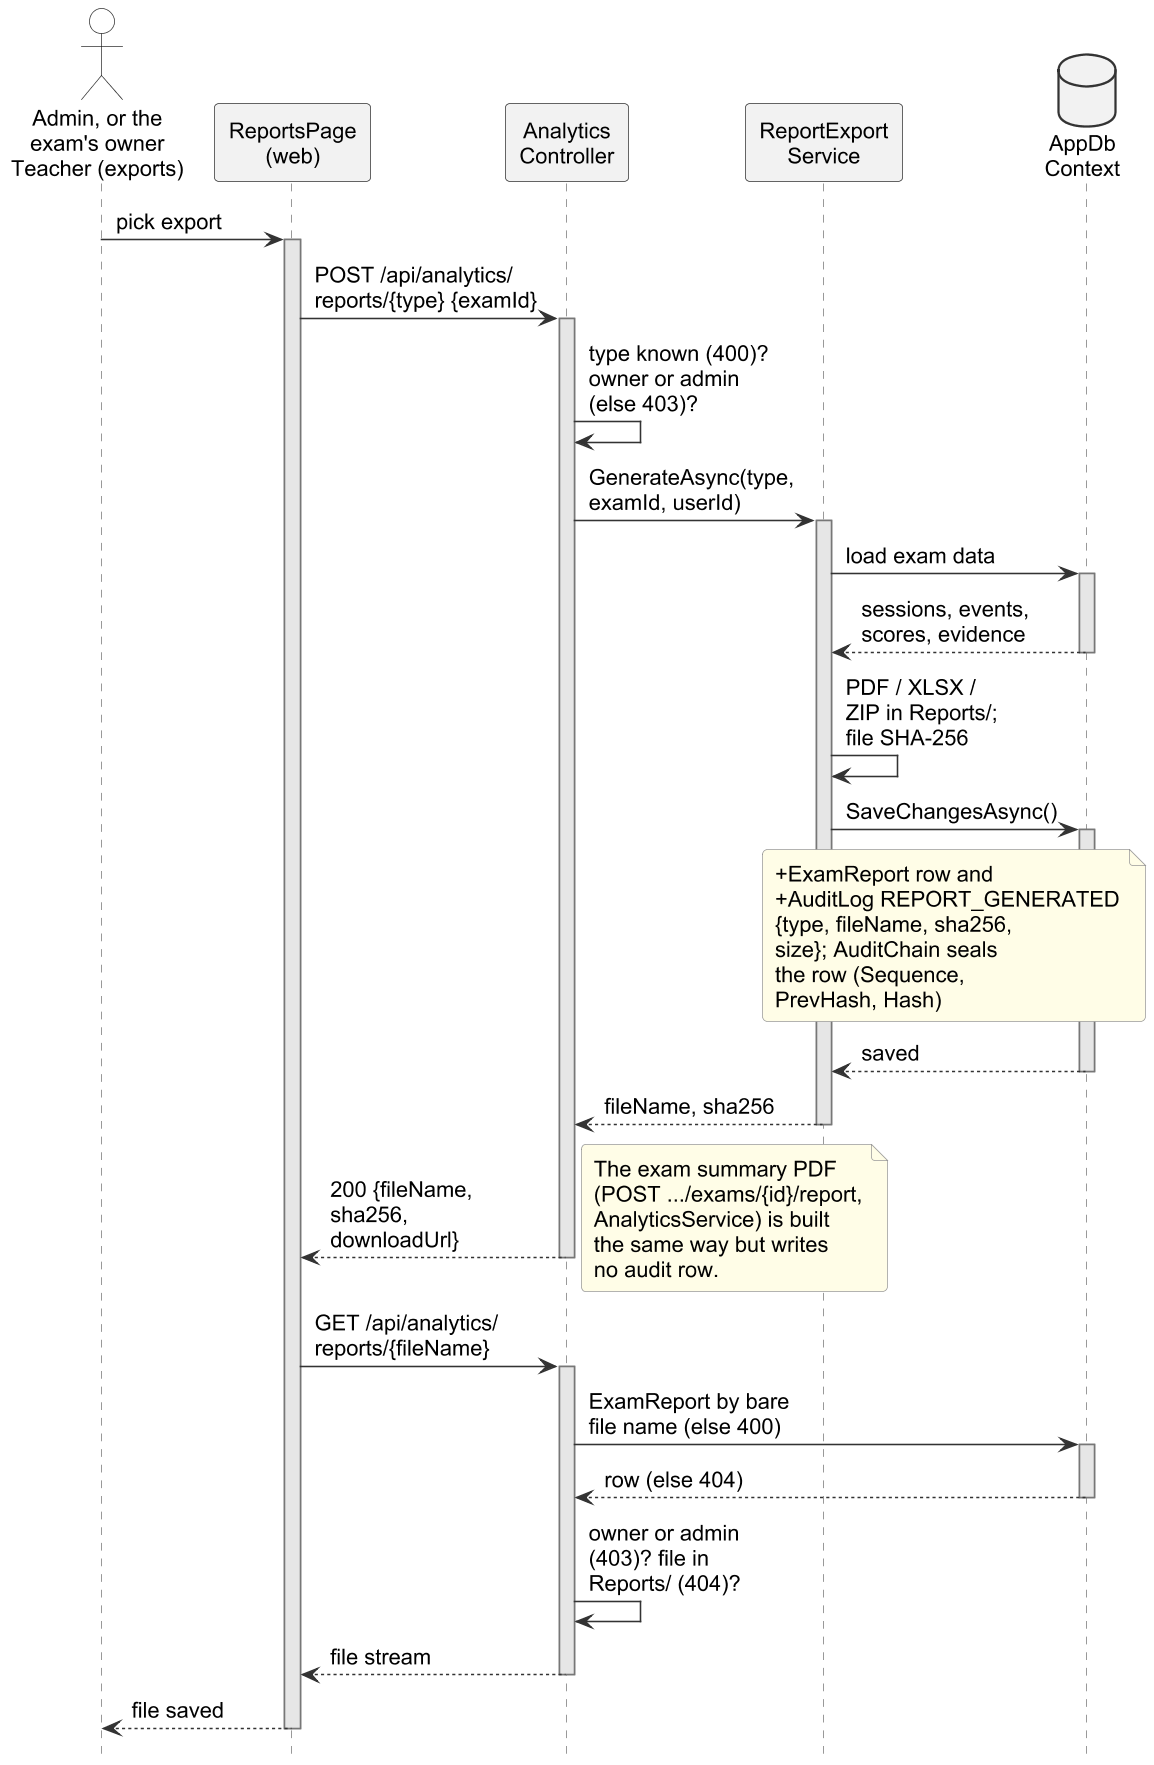
\includegraphics[width=0.90\linewidth,height=621pt,keepaspectratio]{Figures/seq_audit.png}
\caption{Sequence Diagram of Report Export and Audit-Chain Verification (a): Export and Download}
\label{fig:seq_audit}
\end{figure}

\DiagramBarrier
\begin{figure}[H]
\centering
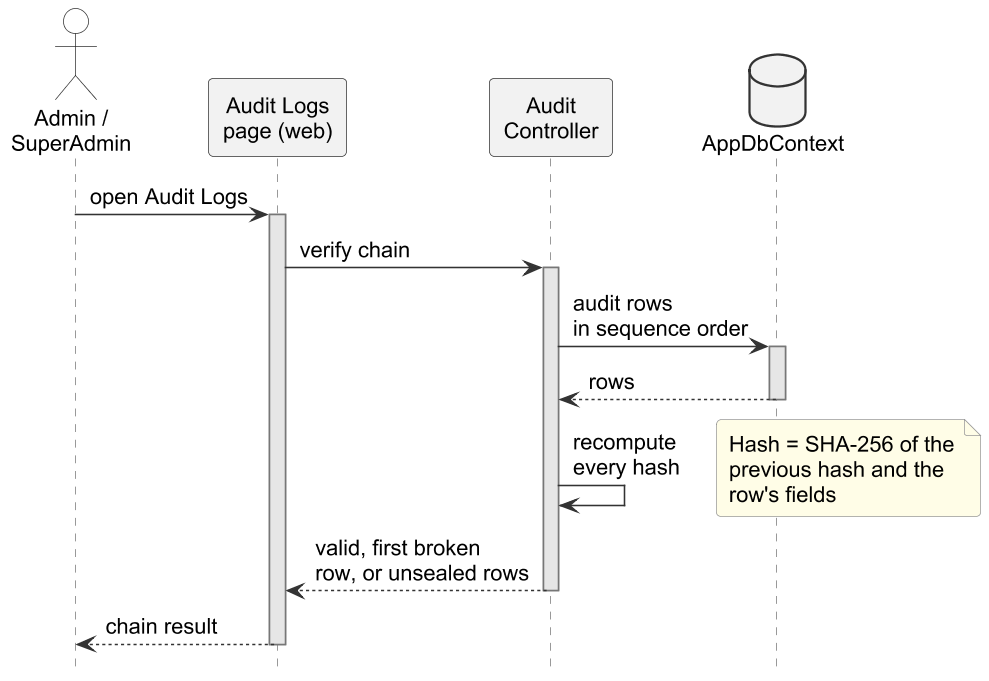
\includegraphics[width=0.70\linewidth,height=325pt,keepaspectratio]{Figures/seq_audit_b.png}
\caption{Sequence Diagram of Report Export and Audit-Chain Verification (b): Chain Verification}
\label{fig:seq_audit_b}
\end{figure}

\DiagramBarrier
\subsubsection{User Management and Eligibility (M7, M9; UC-20, UC-23, UC-25, UC-27)}
\begin{sloppypar}
Administrators manage accounts on the Users page through \texttt{UsersController}. An account is created on its own or in a batch that the page parses from a CSV file; the server skips each bad row with its line and reason and audits the batch as \texttt{USERS\_IMPORTED} (Figures~\ref{fig:seq_users} and~\ref{fig:seq_users_b}). When an Admin creates or acts on an Admin or SuperAdmin account, a single-account call is refused with 403 \texttt{SUPERADMIN\_REQUIRED} and a \texttt{PRIVILEGED\_ACCOUNT\_DENIED} entry is saved at once, while such a row in an import is skipped.
\end{sloppypar}

\begin{sloppypar}
A device-binding reset and a forced logout both revoke the user's refresh tokens and sessions and save the change with its audit entry (\texttt{DEVICE\_BINDING\_RESET} or \texttt{FORCE\_LOGOUT}), so the user's next request is refused even with an unexpired JWT (Figures~\ref{fig:seq_users_c} and~\ref{fig:seq_users_d}). A forced logout also removes the user from any live-monitor groups.
\end{sloppypar}

\begin{figure}[p]
\centering
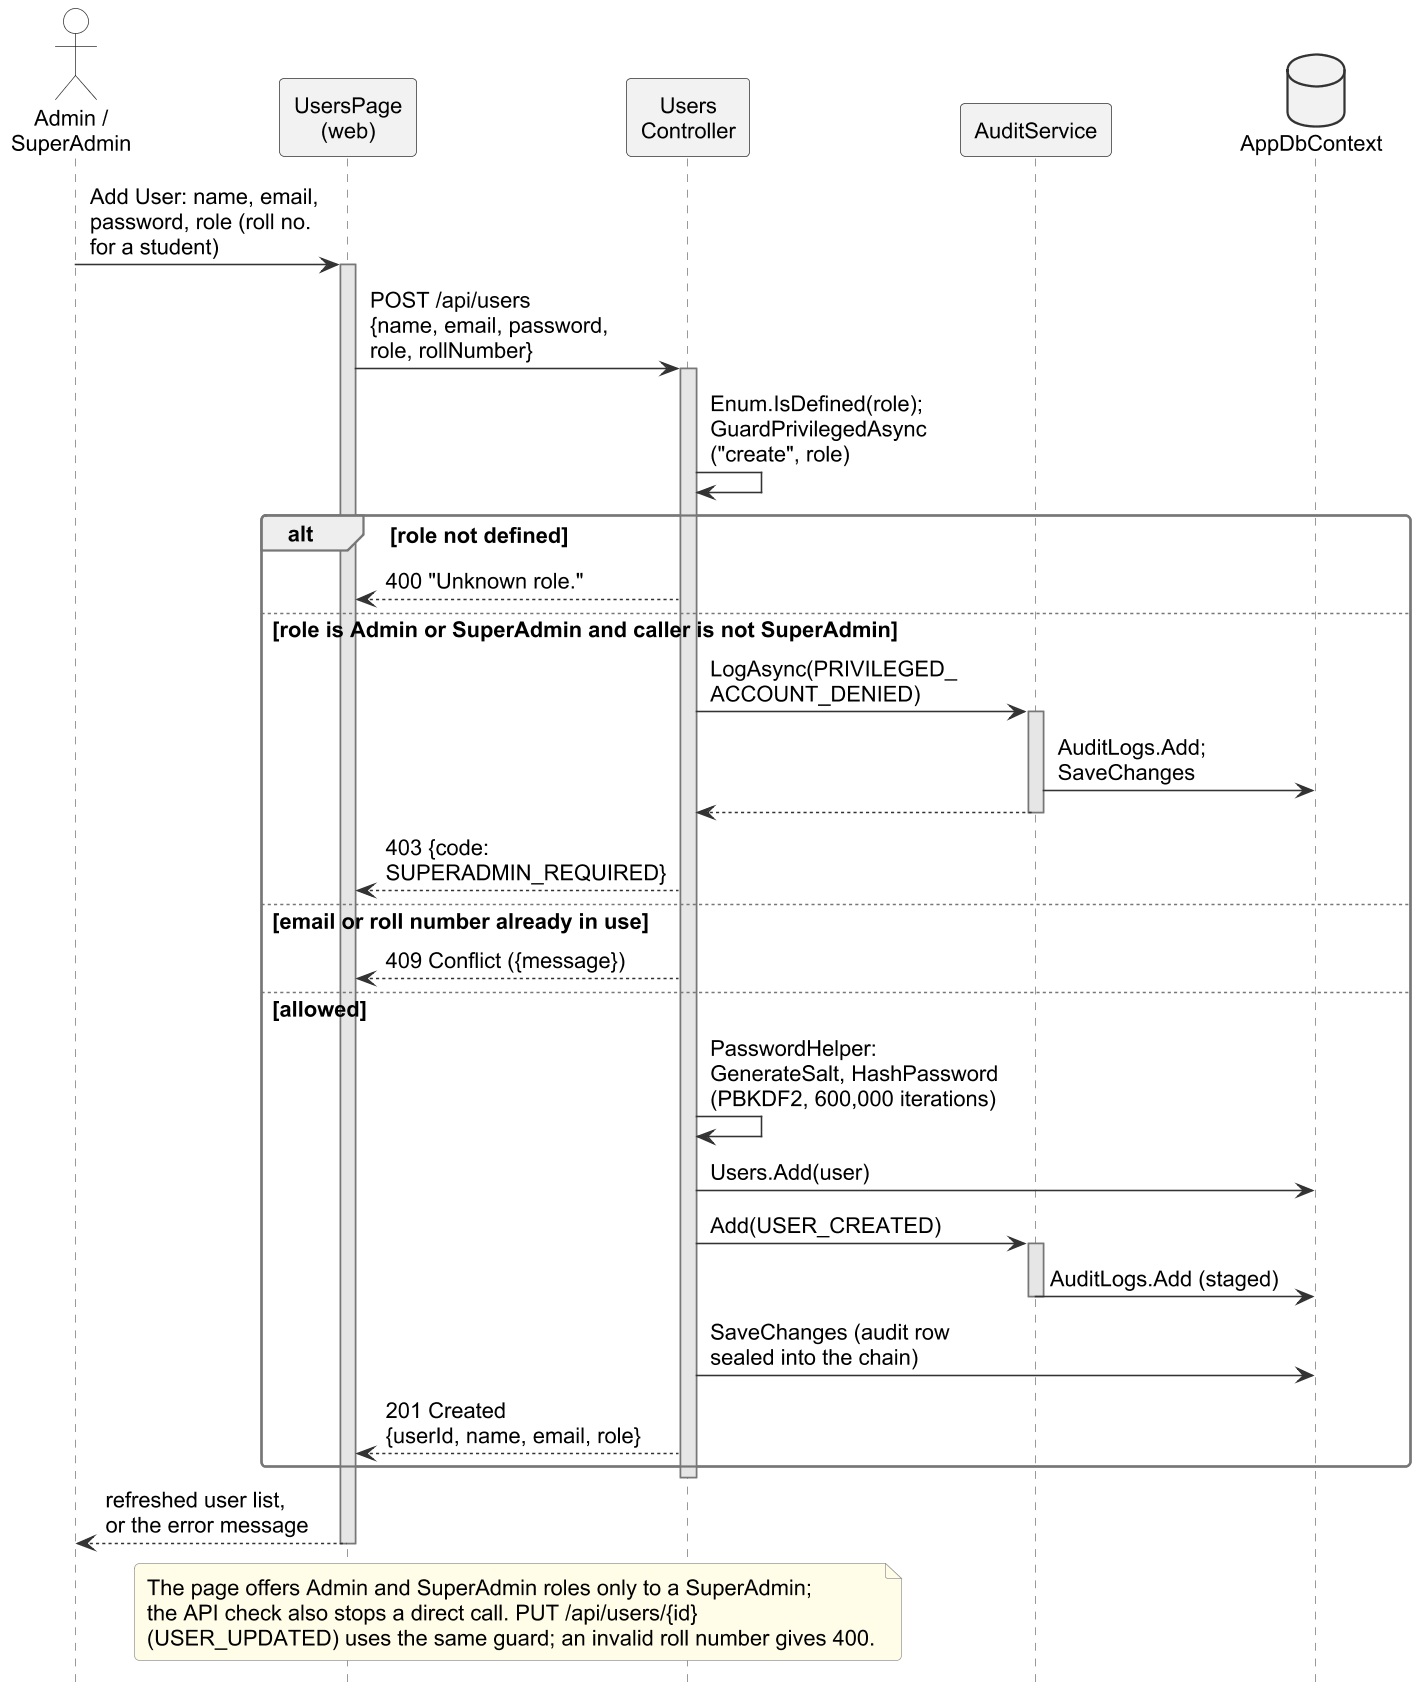
\includegraphics[width=\linewidth,height=560pt,keepaspectratio]{Figures/seq_users.png}
\caption{Sequence Diagram of User and Role Management (a): Creating an Account}
\label{fig:seq_users}
\end{figure}

\begin{figure}[H]
\centering
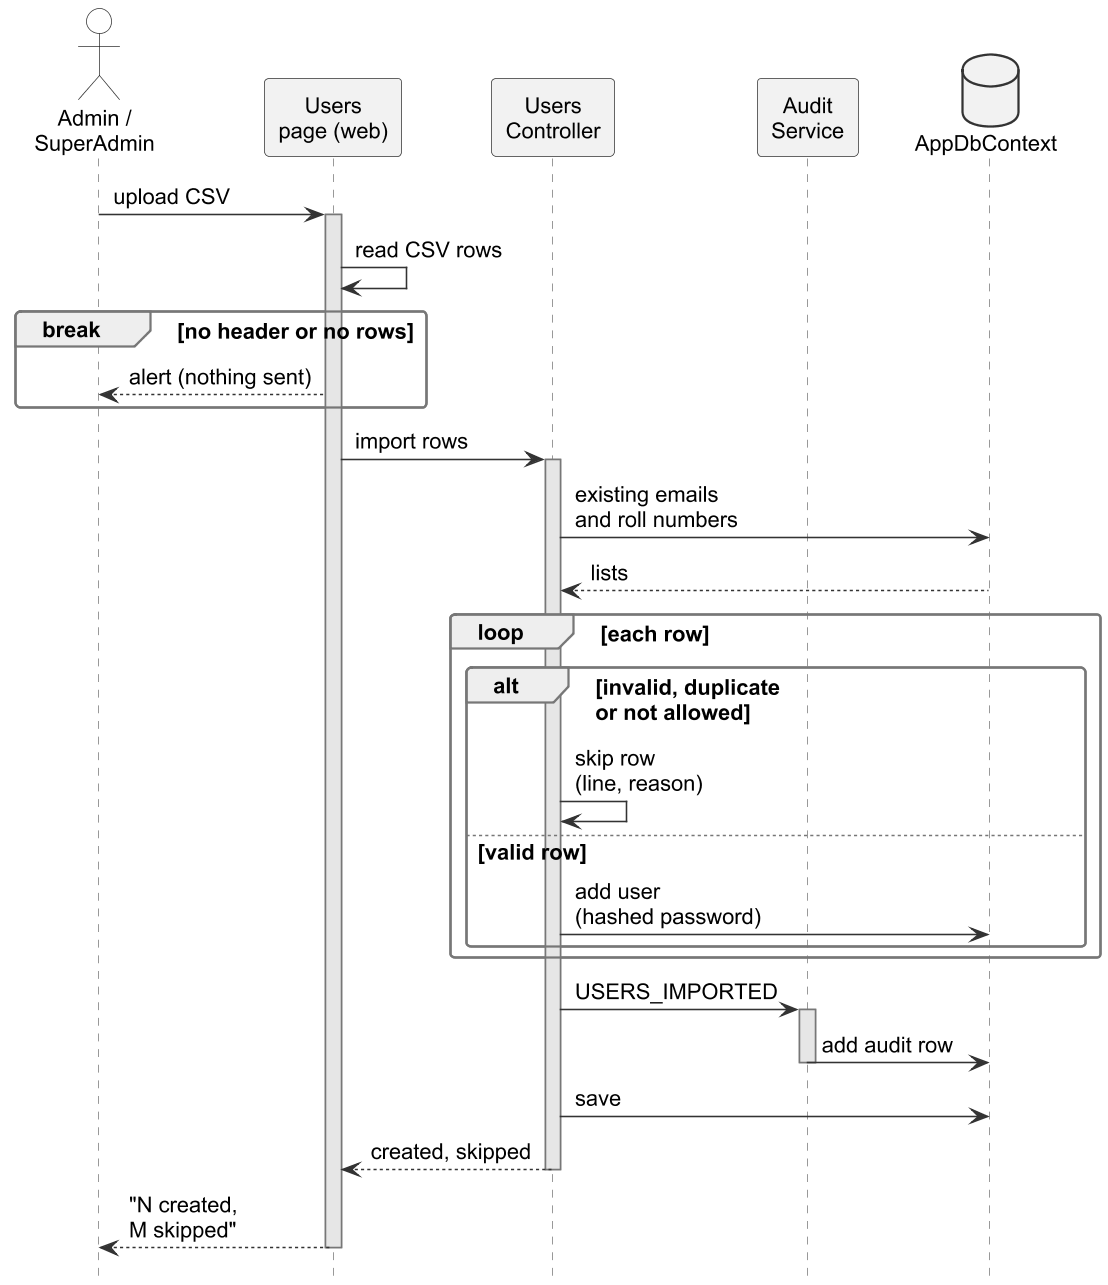
\includegraphics[width=\linewidth,height=460pt,keepaspectratio]{Figures/seq_users_b.png}
\caption{Sequence Diagram of User and Role Management (b): CSV Import}
\label{fig:seq_users_b}
\end{figure}

\begin{figure}[H]
\centering
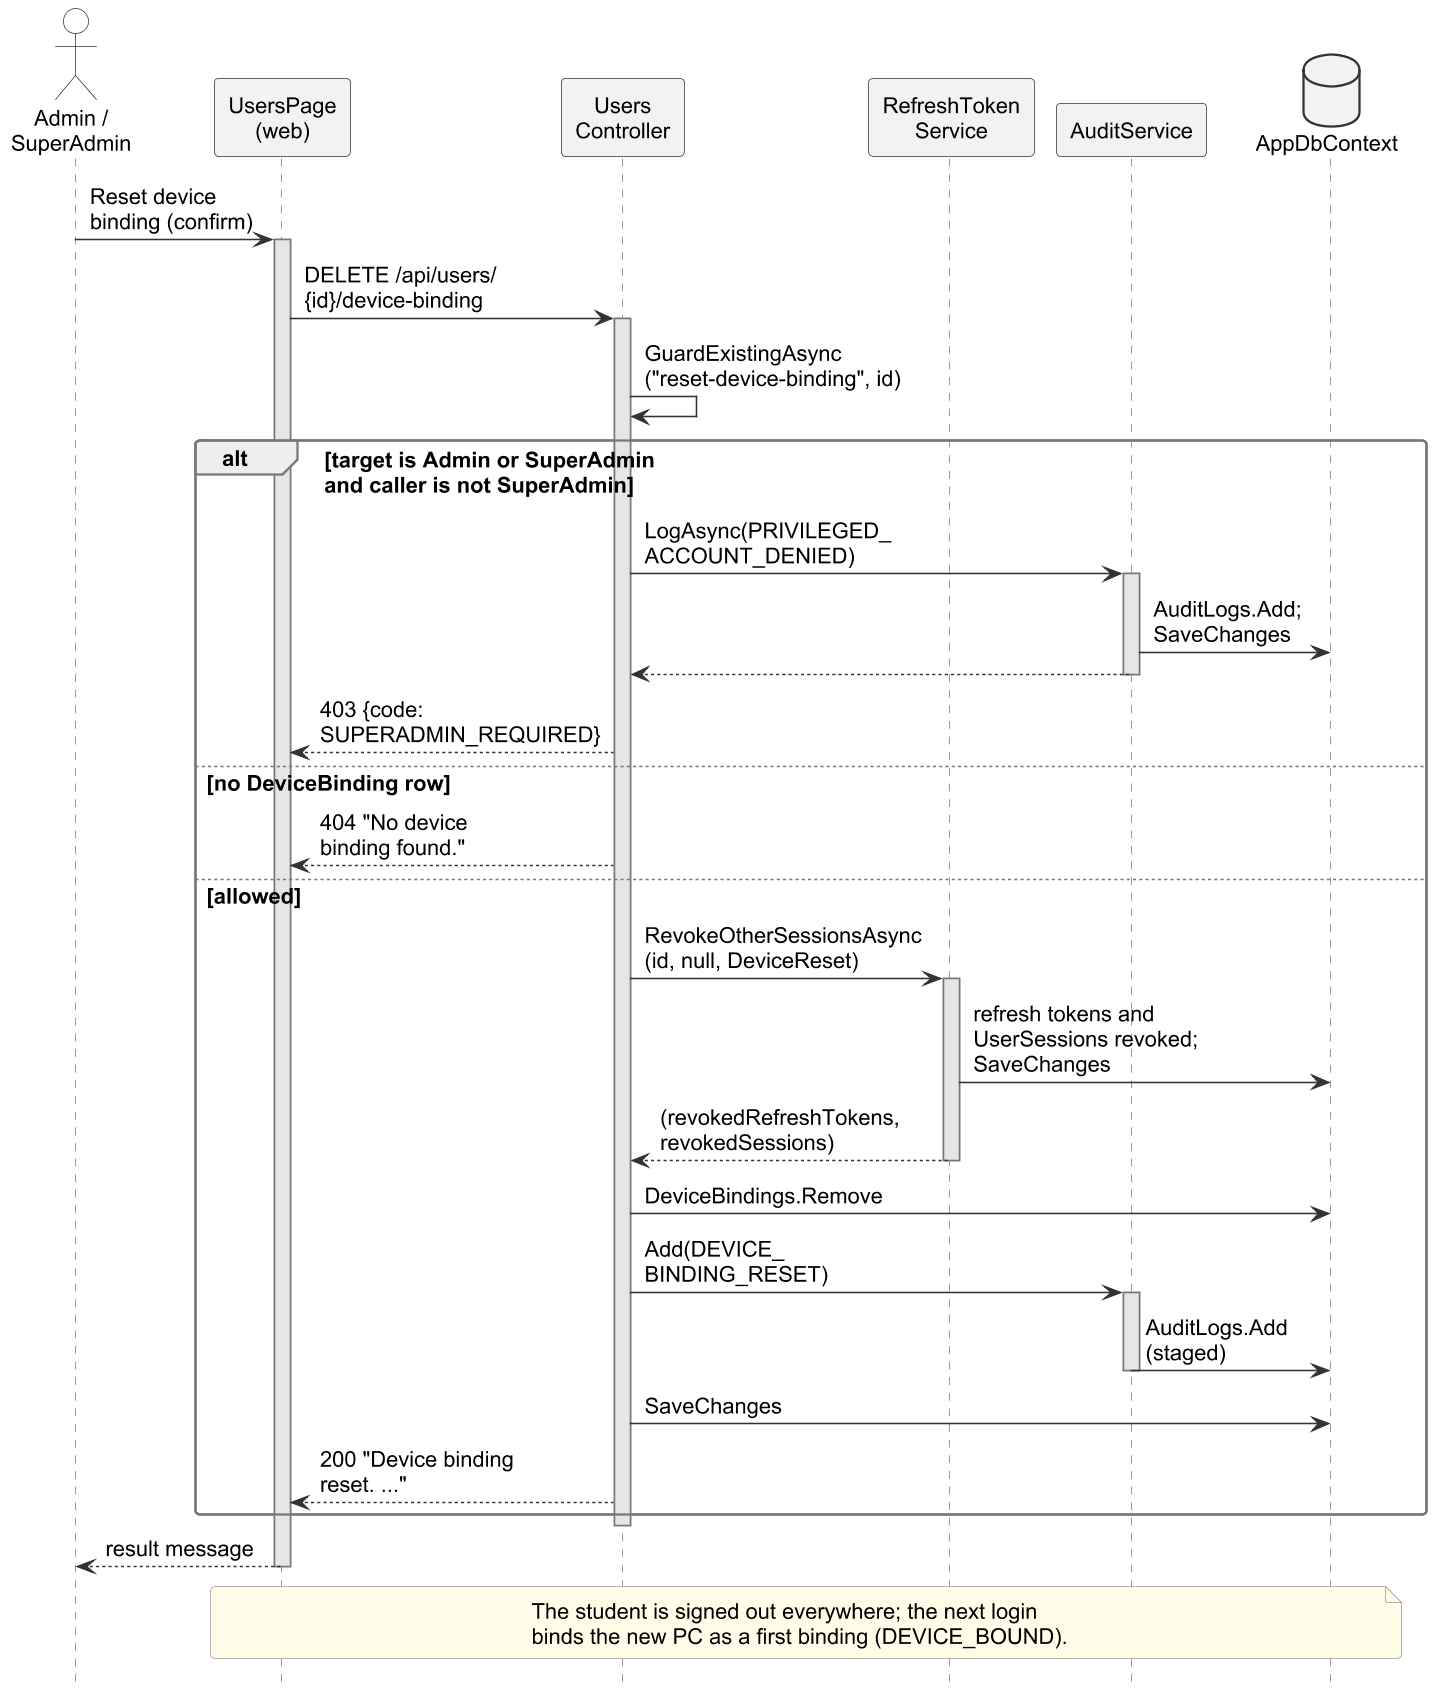
\includegraphics[width=\linewidth,height=535pt,keepaspectratio]{Figures/seq_users_c.png}
\caption{Sequence Diagram of User and Role Management (c): Device-Binding Reset}
\label{fig:seq_users_c}
\end{figure}

\begin{figure}[H]
\centering
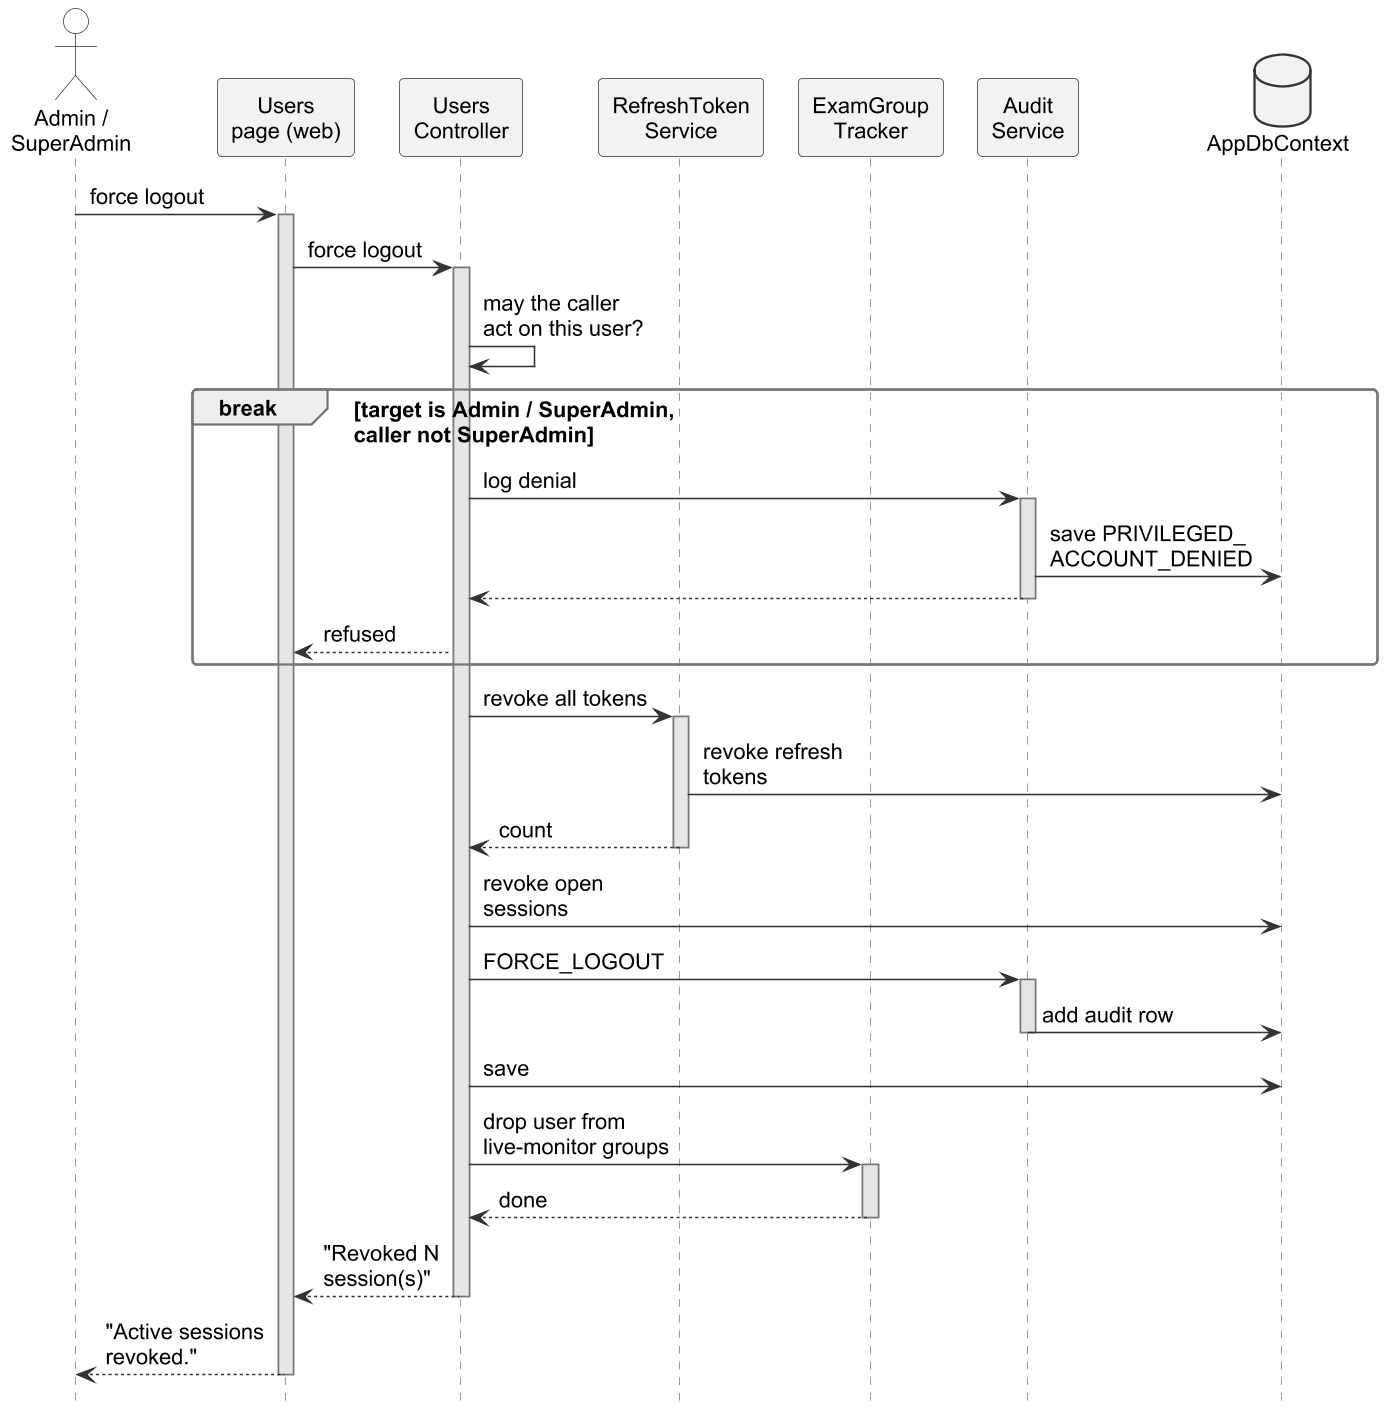
\includegraphics[width=\linewidth,height=515pt,keepaspectratio]{Figures/seq_users_d.png}
\caption{Sequence Diagram of User and Role Management (d): Force Logout}
\label{fig:seq_users_d}
\end{figure}

\begin{sloppypar}
On the Eligibility page a teacher uploads the section's attendance CSV (at most 1~MB) to \texttt{AttendanceController}, which stores each student's total and attended classes and reports rejected rows by line (Figure~\ref{fig:seq_eligibility}). Recalculation (Figure~\ref{fig:seq_eligibility_b}) passes every assignment without a manual override to \texttt{EligibilityCalculator.Decide}, which compares the unrounded attendance percentage with the exam's \texttt{MinAttendancePercent} (75\% by default); a student with no attendance data keeps the earlier decision. A manual change (Figure~\ref{fig:seq_eligibility_c}) is audited per student as \texttt{ELIGIBILITY\_OVERRIDDEN}, and later recalculations skip that student until the override is cleared.
\end{sloppypar}

\begin{figure}[p]
\centering
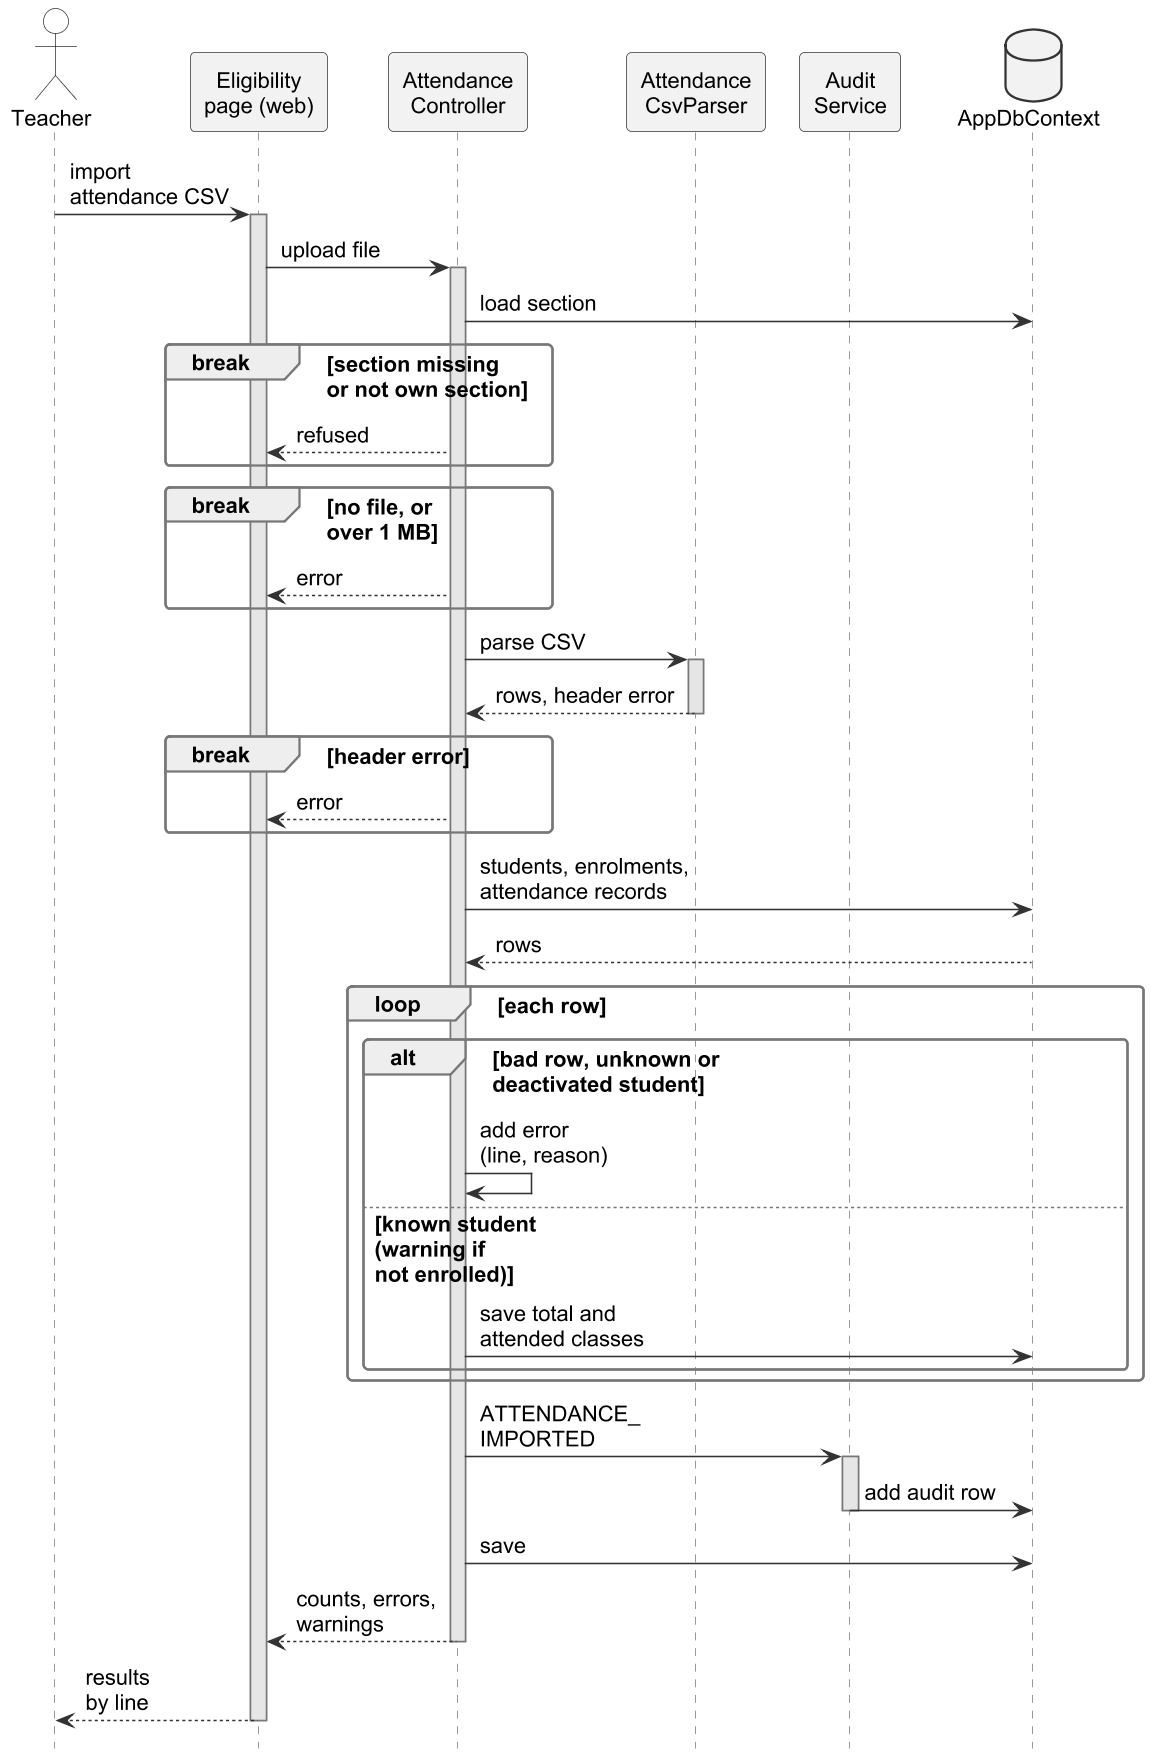
\includegraphics[width=\linewidth,height=628pt,keepaspectratio]{Figures/seq_eligibility.png}
\caption{Sequence Diagram of Attendance Import and Eligibility (a): Attendance Import}
\label{fig:seq_eligibility}
\end{figure}

\begin{figure}[p]
\centering
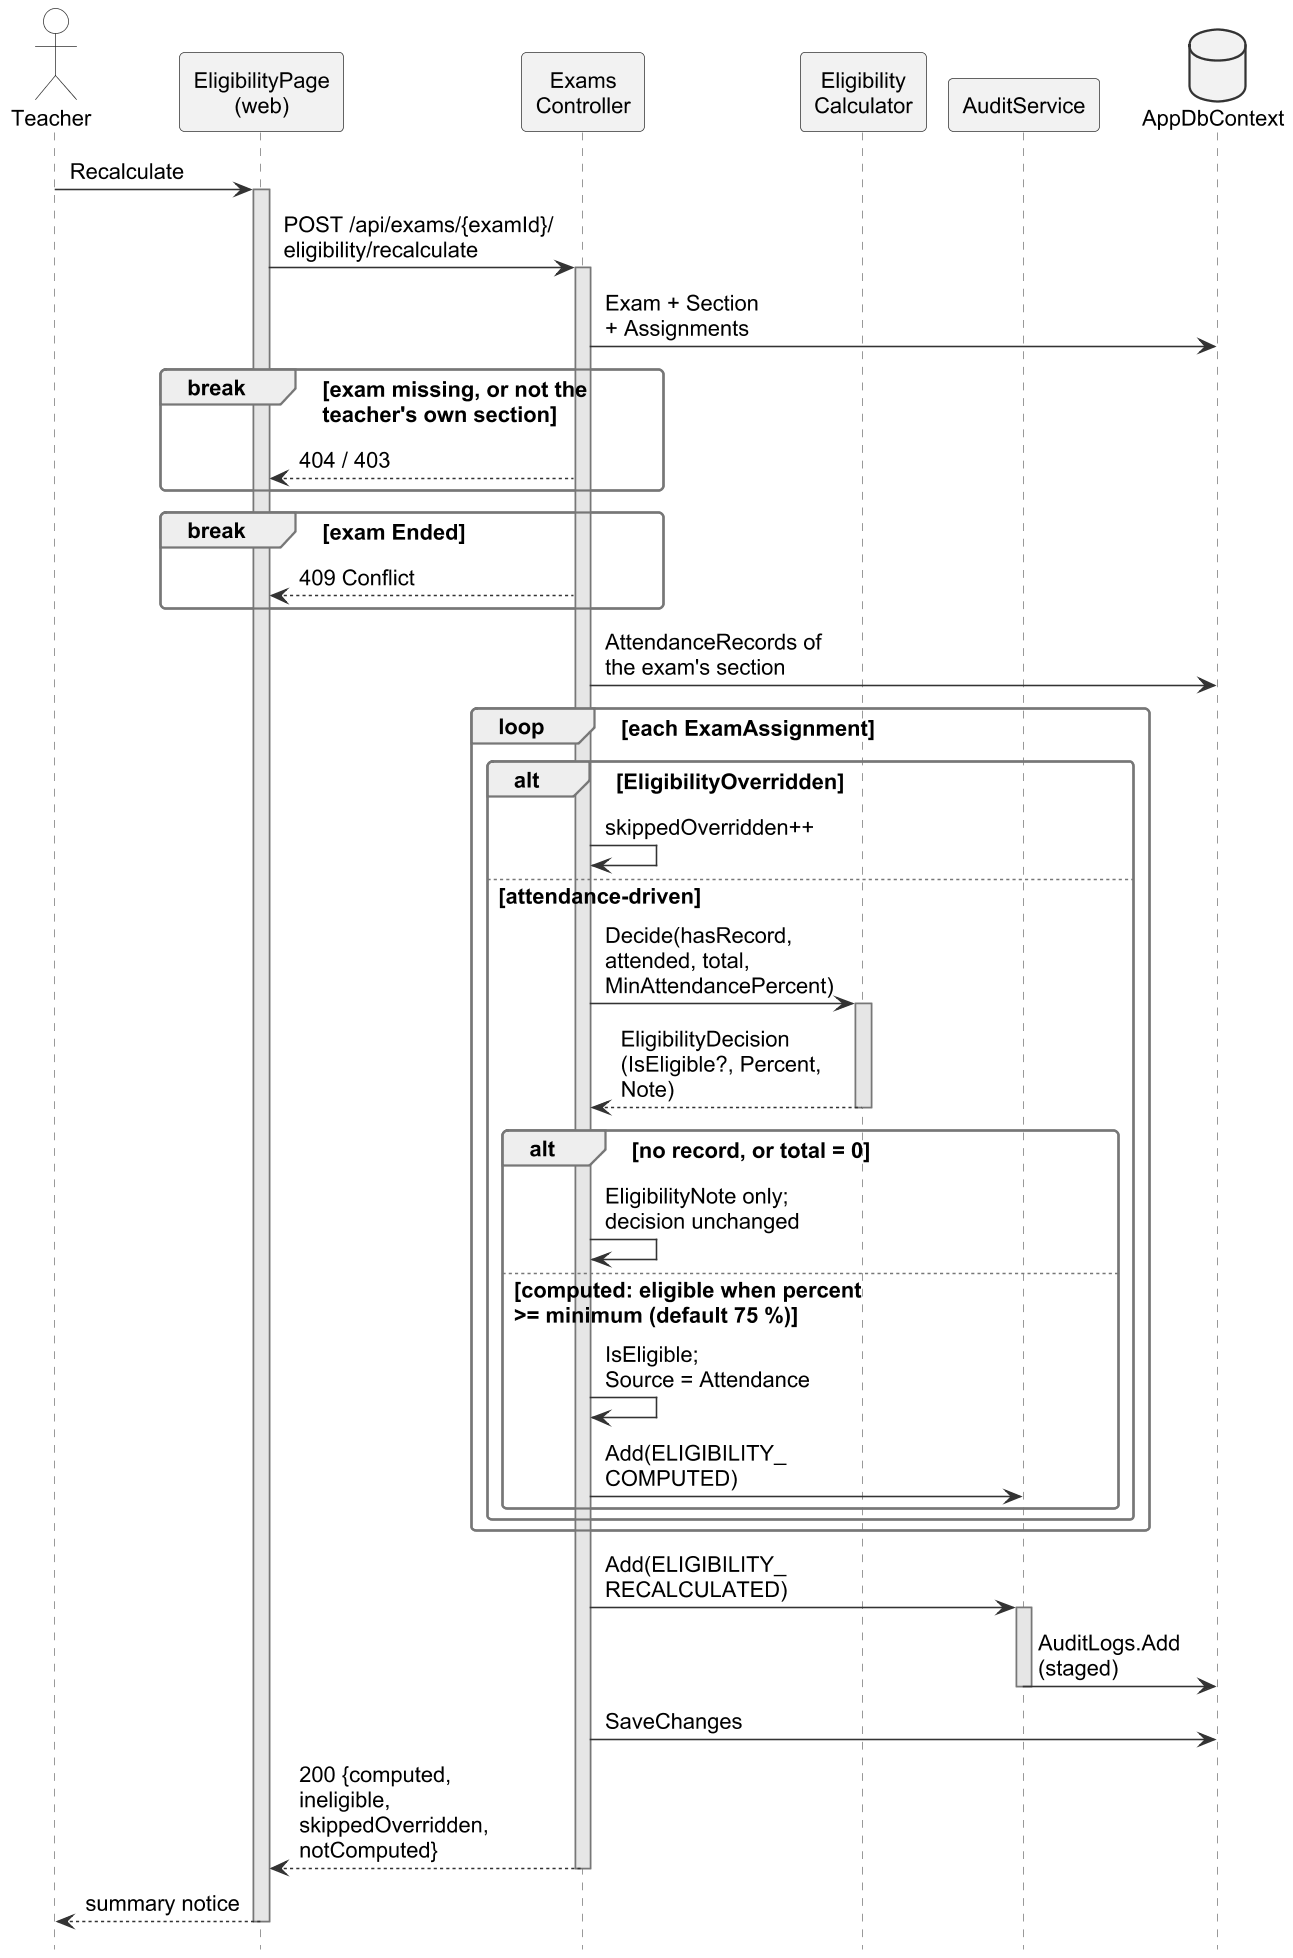
\includegraphics[width=\linewidth,height=628pt,keepaspectratio]{Figures/seq_eligibility_b.png}
\caption{Sequence Diagram of Attendance Import and Eligibility (b): Recalculation from Attendance}
\label{fig:seq_eligibility_b}
\end{figure}

\begin{figure}[H]
\centering
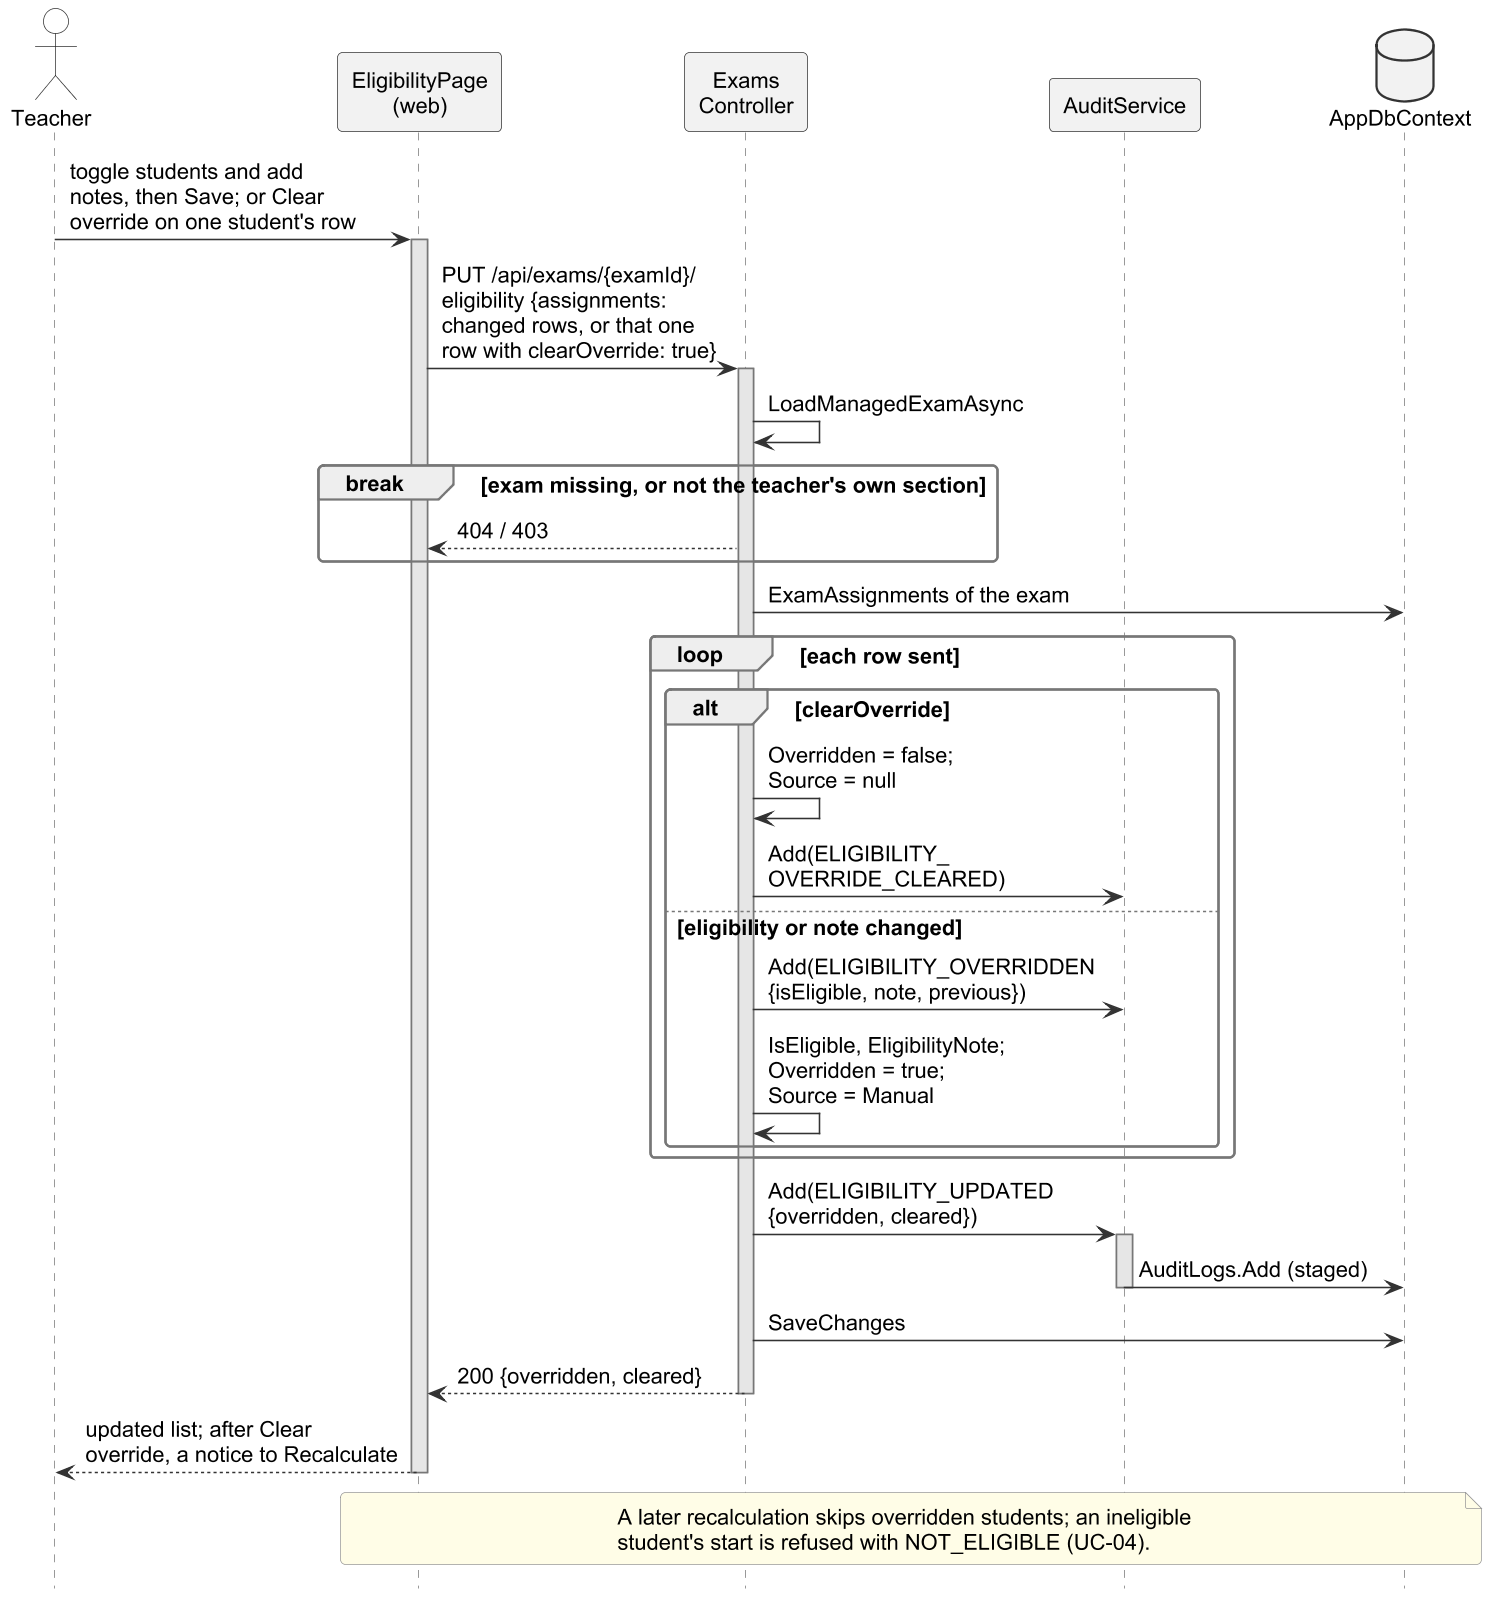
\includegraphics[width=\linewidth,height=530pt,keepaspectratio]{Figures/seq_eligibility_c.png}
\caption{Sequence Diagram of Attendance Import and Eligibility (c): Manual Override}
\label{fig:seq_eligibility_c}
\end{figure}

\renewcommand{\floatpagefraction}{0.5}
\renewcommand{\topfraction}{0.7}
\renewcommand{\textfraction}{0.2}

\chapter{SYSTEM INTERFACE AND PHYSICAL DESIGN}
\label{chap:system_interface_physical_design}

This chapter shows what each user sees and how the data is stored. Section~\ref{sec:system_user_interfaces} follows an exam from start to finish: the student's desktop client, exam set-up, live invigilation, evaluation, administration and the student portal. Section~\ref{sec:physical_tables} gives one table for each entity of the ERD (Figure~\ref{fig:erd_diagram}) with its fields, data types and keys.

\section{System User Interfaces}
\label{sec:system_user_interfaces}
SmartExam has two front ends: a WPF desktop client (.NET~9) in which students sit the exam, and a React web panel with one route group per role (\texttt{/admin}, \texttt{/teacher}, \texttt{/invigilator}, \texttt{/student}). Both follow common usability heuristics: the system status is always visible (connection, last save, tile status), final actions such as submit and force-submit ask for confirmation, and controls look the same across roles \cite{nielsen_heuristics}. The web figures are captured from the running panel by a Playwright script (\texttt{Admin\_Web\_Panel/tests/docs}) against the in-memory backend with the seeded demo data; a scripted client plays the desktop app and uploads the screen captures. The desktop figures are rendered off-screen from the client's own XAML (Extensible Application Markup Language) views with values from the same run, because the lockdown window cannot be captured safely on a development PC. The student, invigilation and evaluation figures show one exam, the Mid-Term Lab Exam (Demo), in Enforce mode with a required system check and webcam.

% Section 6.1 is mostly screenshots: let a tall figure share a page with text
% (book defaults are restored before Section 6.2).
\renewcommand{\topfraction}{0.9}\renewcommand{\bottomfraction}{0.9}
\renewcommand{\textfraction}{0.07}\renewcommand{\floatpagefraction}{0.8}
\subsection{Student Desktop Client}
The student signs in with email or roll number (Figure~\ref{fig:ui_student_login}). The client reads the BIOS, system-disk and baseboard serials; the server hashes them with SHA-256 into the hardware ID (HWID) and keeps only the hash in \texttt{DeviceBindings}, so a login from another PC is refused (FR1). The window has one field for the email or roll number (here \texttt{BSCS-21-001}) and one for the password. The note above \emph{Sign In} warns that the device will be bound to the account, and the box at the bottom shows the connection state (\emph{Connected to server}), so the student knows before signing in that the server can be reached.

\begin{figure}[tbp]
\centering
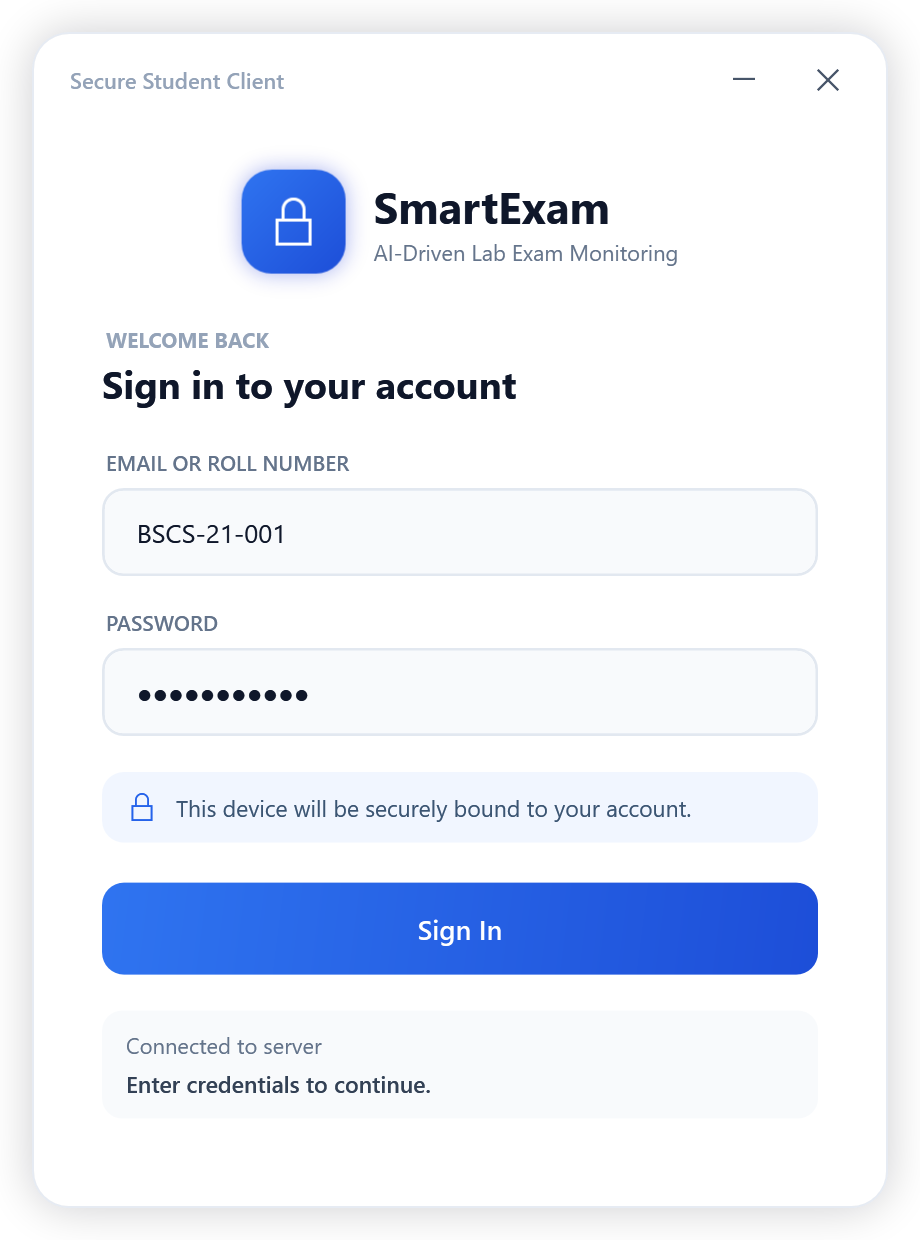
\includegraphics[width=\linewidth,height=0.9\textheight,keepaspectratio]{Figures/ui_student_login.png}
\caption{Desktop Client Login}
\label{fig:ui_student_login}
\end{figure}
\SoftBarrierN

The exam dashboard shows the student's current assigned exam with its instructions and permitted applications (Figure~\ref{fig:ui_student_diagnostics}); a side panel, not shown, gives the remaining time, lab, seat, attendance check-in and invigilator messages. An ineligible student still sees the exam, with \emph{Start Exam} disabled and the reason shown (FR3). In the figure, the blue header gives the exam title, its status (Active) and the teacher (Dr. Ahmed), and the permitted applications are \texttt{code.exe} and \texttt{codeblocks.exe}. In the \emph{System Check} list a green tick is a passed check, a dash is a skipped check and a red cross is a failed check with a \emph{Retry} button beside it. The dashboard runs the readiness checks (FR2): network, clock skew, screen capture, webcam, microphone, secure mode (monitors, remote session, virtual machine, keyboard hook) and disk space. This exam needs the webcam but not the microphone, so the microphone is skipped. Secure mode fails because a second monitor is attached, and since the exam requires the check (\texttt{RequireReadiness}), \emph{Start Exam} stays disabled until a passing check less than 30 minutes old exists.

\begin{figure}[tbp]
\centering
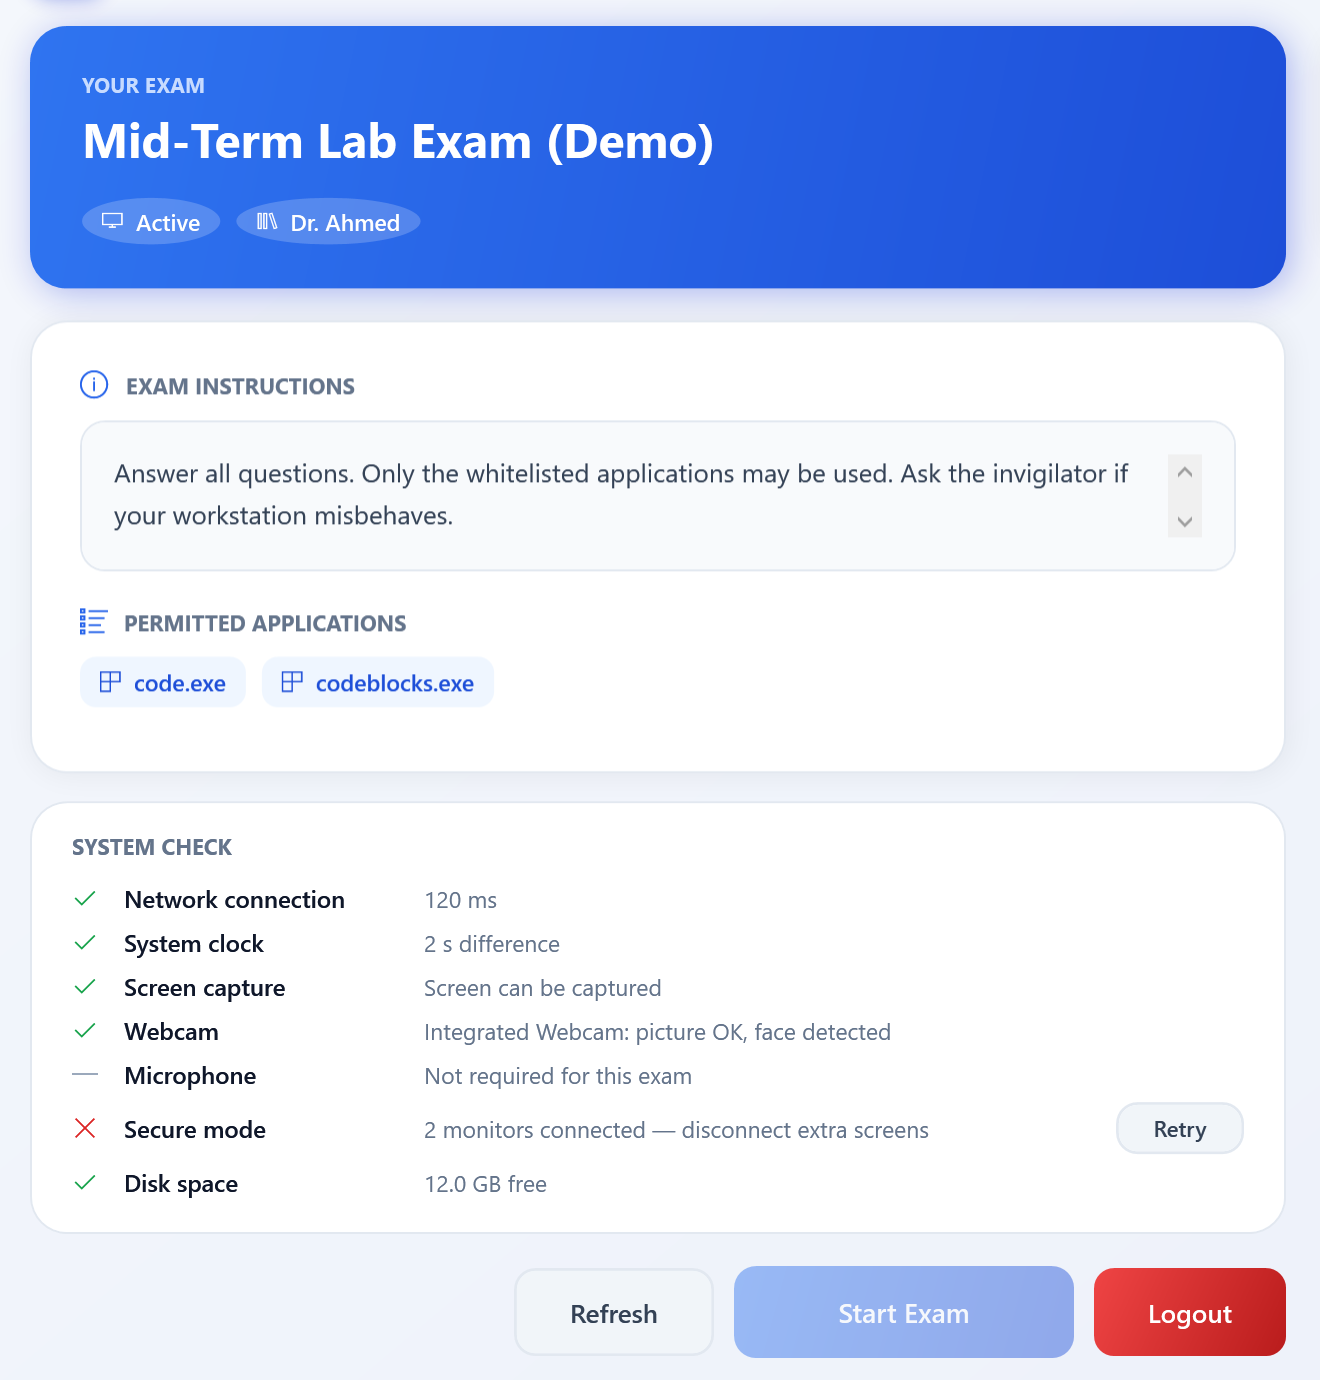
\includegraphics[width=\linewidth,height=472pt,keepaspectratio]{Figures/ui_student_diagnostics.png}
\caption{Exam Dashboard with Readiness Checks}
\label{fig:ui_student_diagnostics}
\end{figure}
\SoftBarrierN

The exam window (Figures~\ref{fig:ui_student_workspace} and~\ref{fig:ui_student_workspace_b}) opens maximised, borderless and topmost (FR4). A low-level keyboard hook blocks the Windows and menu keys, PrintScreen, Alt+Tab, Alt+F4, Alt+Esc, Ctrl+Esc and Ctrl+Shift+Esc, while guard services watch processes, the clipboard and newly mounted USB storage devices. The student picks a question from the list on the left and types the answer; coding answers go into a monospace text box. Every edit is written within about a second to an AES-256-GCM encrypted backup on disk and saved to the server 10~s after the first unsaved edit; saves made offline are queued and replayed (FR6). The footer shows the last save time.

The window is printed in two parts. Part~(a) is the left side panel: the exam title with the number of answered questions (2 of 3), the question list (1 Coding, 2 Theory, 3 Multiple Choice) with a green dot for each answered question, and the footer \emph{Saved 3:35:32 PM}; the empty middle of the panel is cut out. Part~(b) is the question area: the countdown timer (01:27:18) in the header, the type and marks of Question~1 (Coding, 20 marks), the C++ answer in the \emph{Your Code} box, and the \emph{Previous}, \emph{Next} and \emph{Submit Exam} buttons. So the student can always see how much is answered, how much time is left and when the work was last saved.

\begin{figure}[tbp]
\centering
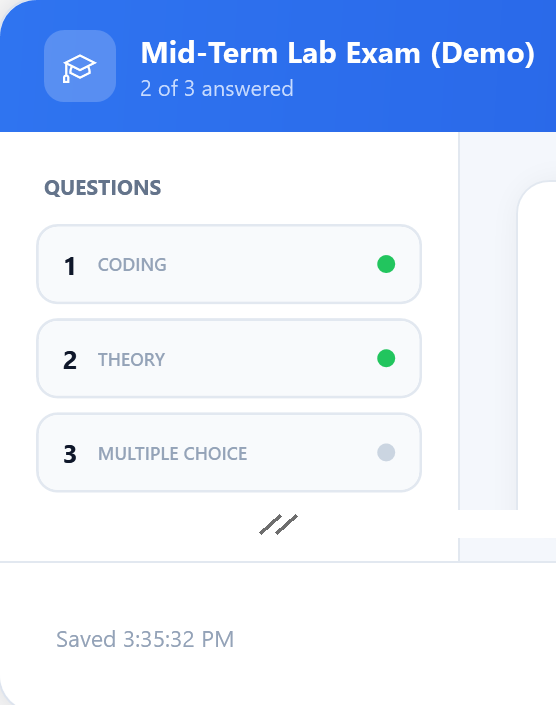
\includegraphics[width=0.5\linewidth]{Figures/ui_student_workspace_p1.png}
\caption{Desktop Exam Window (a): Question List and Save Status (Empty Middle Omitted)}
\label{fig:ui_student_workspace}
\end{figure}
\SoftBarrierN

\begin{figure}[tbp]
\centering
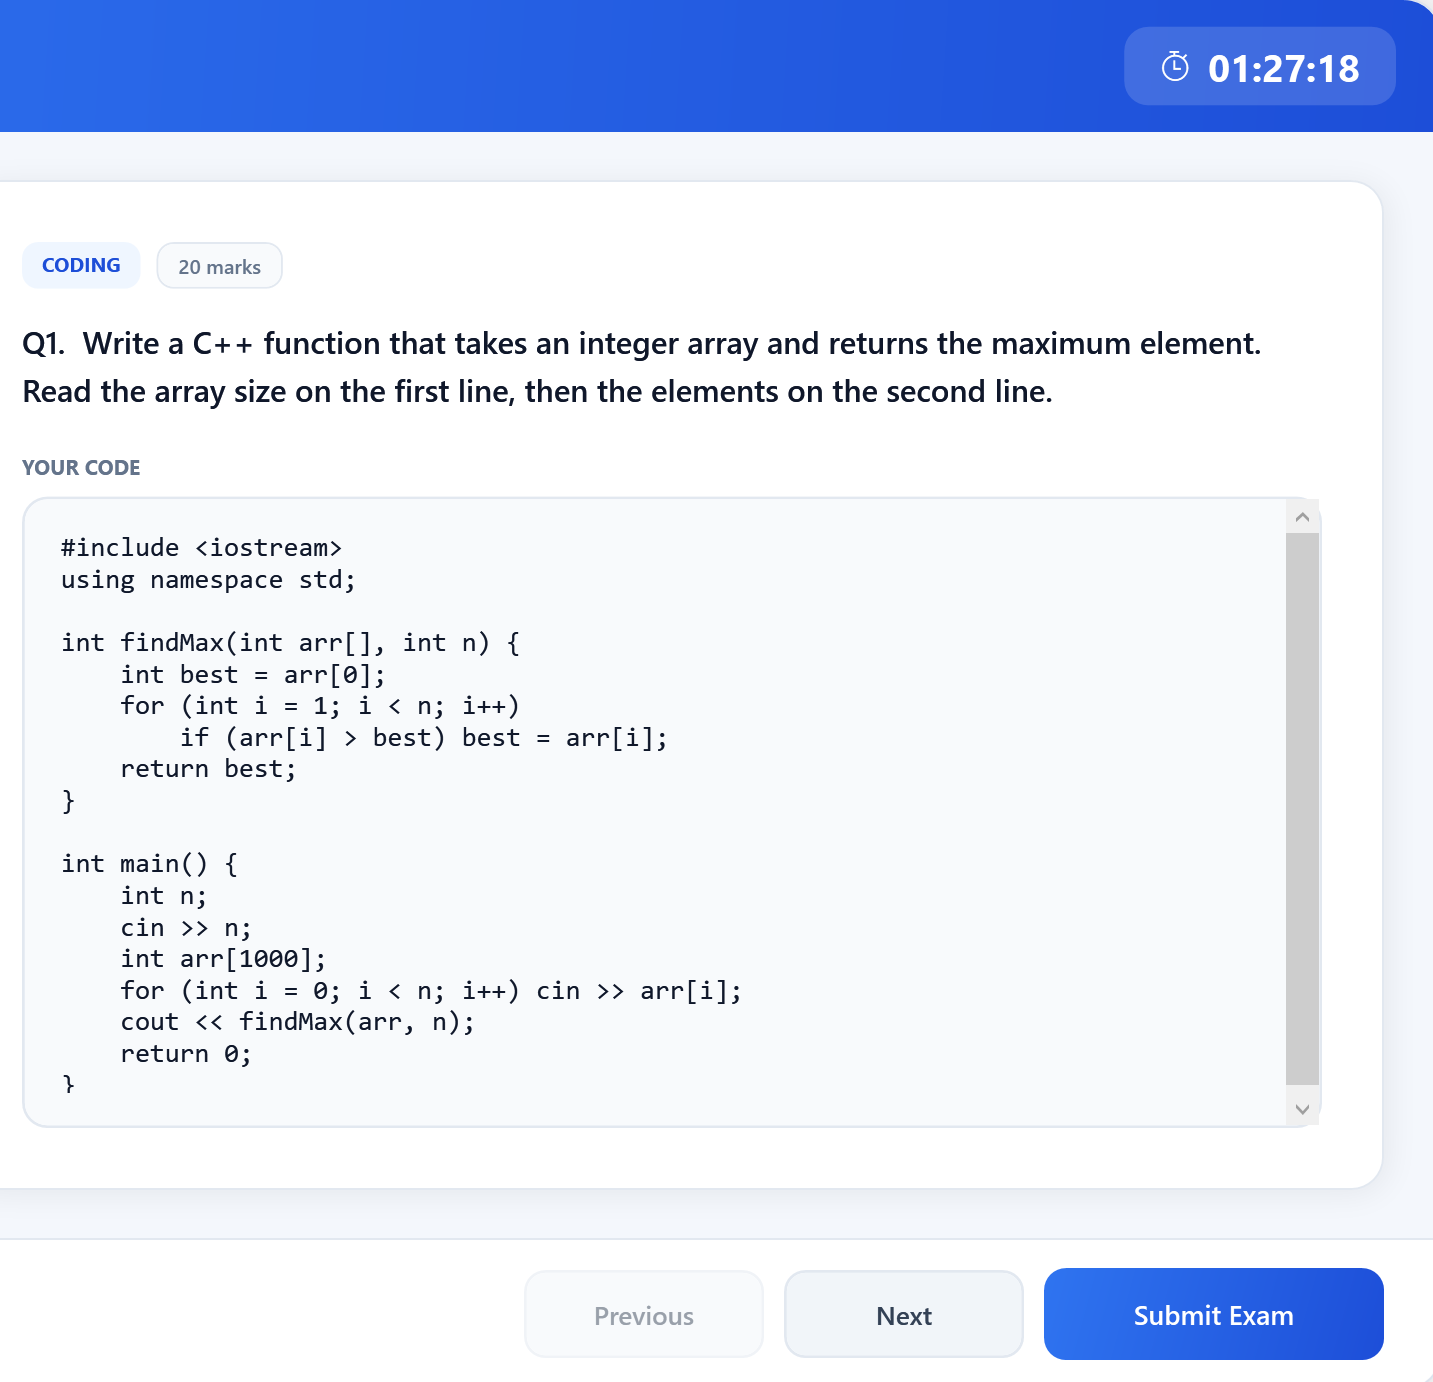
\includegraphics[width=\linewidth]{Figures/ui_student_workspace_p2.png}
\caption{Desktop Exam Window (b): Coding Question, Timer and Answer Box}
\label{fig:ui_student_workspace_b}
\end{figure}
\SoftBarrierN

A warning sent by an invigilator reaches the client in the reply to its next heartbeat (every 10~s) and appears as a banner between the window header and the question (Figure~\ref{fig:ui_student_warning}, the warning sent in Figure~\ref{fig:ui_live_timeline}). The banner shows the title \emph{Proctor Warning} with the time it was sent (15:35), the invigilator's message and an \emph{Acknowledge} button; the empty middle of the wide banner is cut out. The banner stays until the student acknowledges it, further warnings wait in a queue and are shown one by one, and the student's \emph{Acknowledge} is written to the audit log (FR10).

\begin{figure}[tbp]
\centering

\includegraphics[width=\linewidth]{Figures/ui_student_warning_banner.png}
\caption{Invigilator Warning Banner in the Exam Window (Empty Middle Omitted)}
\label{fig:ui_student_warning}
\end{figure}
\SoftBarrierN

\subsection{Exam Setup}
The teacher dashboard (Figure~\ref{fig:ui_teacher_dashboard}) counts the teacher's exams, the running ones and the ended exams waiting for grade review. It lists scheduled exams, including the seeded practice exam, which stays open for a week, with \emph{Manage}, \emph{Edit} and \emph{Delete}, and links each ended exam to \emph{Review Grades}. In the figure, Dr. Ahmed has six exams, one running now and three waiting for review. The left list holds the two scheduled exams, the practice exam (tagged \emph{Practice}) and the End-Term Lab Exam (tagged \emph{Ready}), and the right panel lists the three ended Data Structures exams. The page tells the teacher at a glance what is coming next and what still needs grading.

\begin{figure}[tbp]
\centering
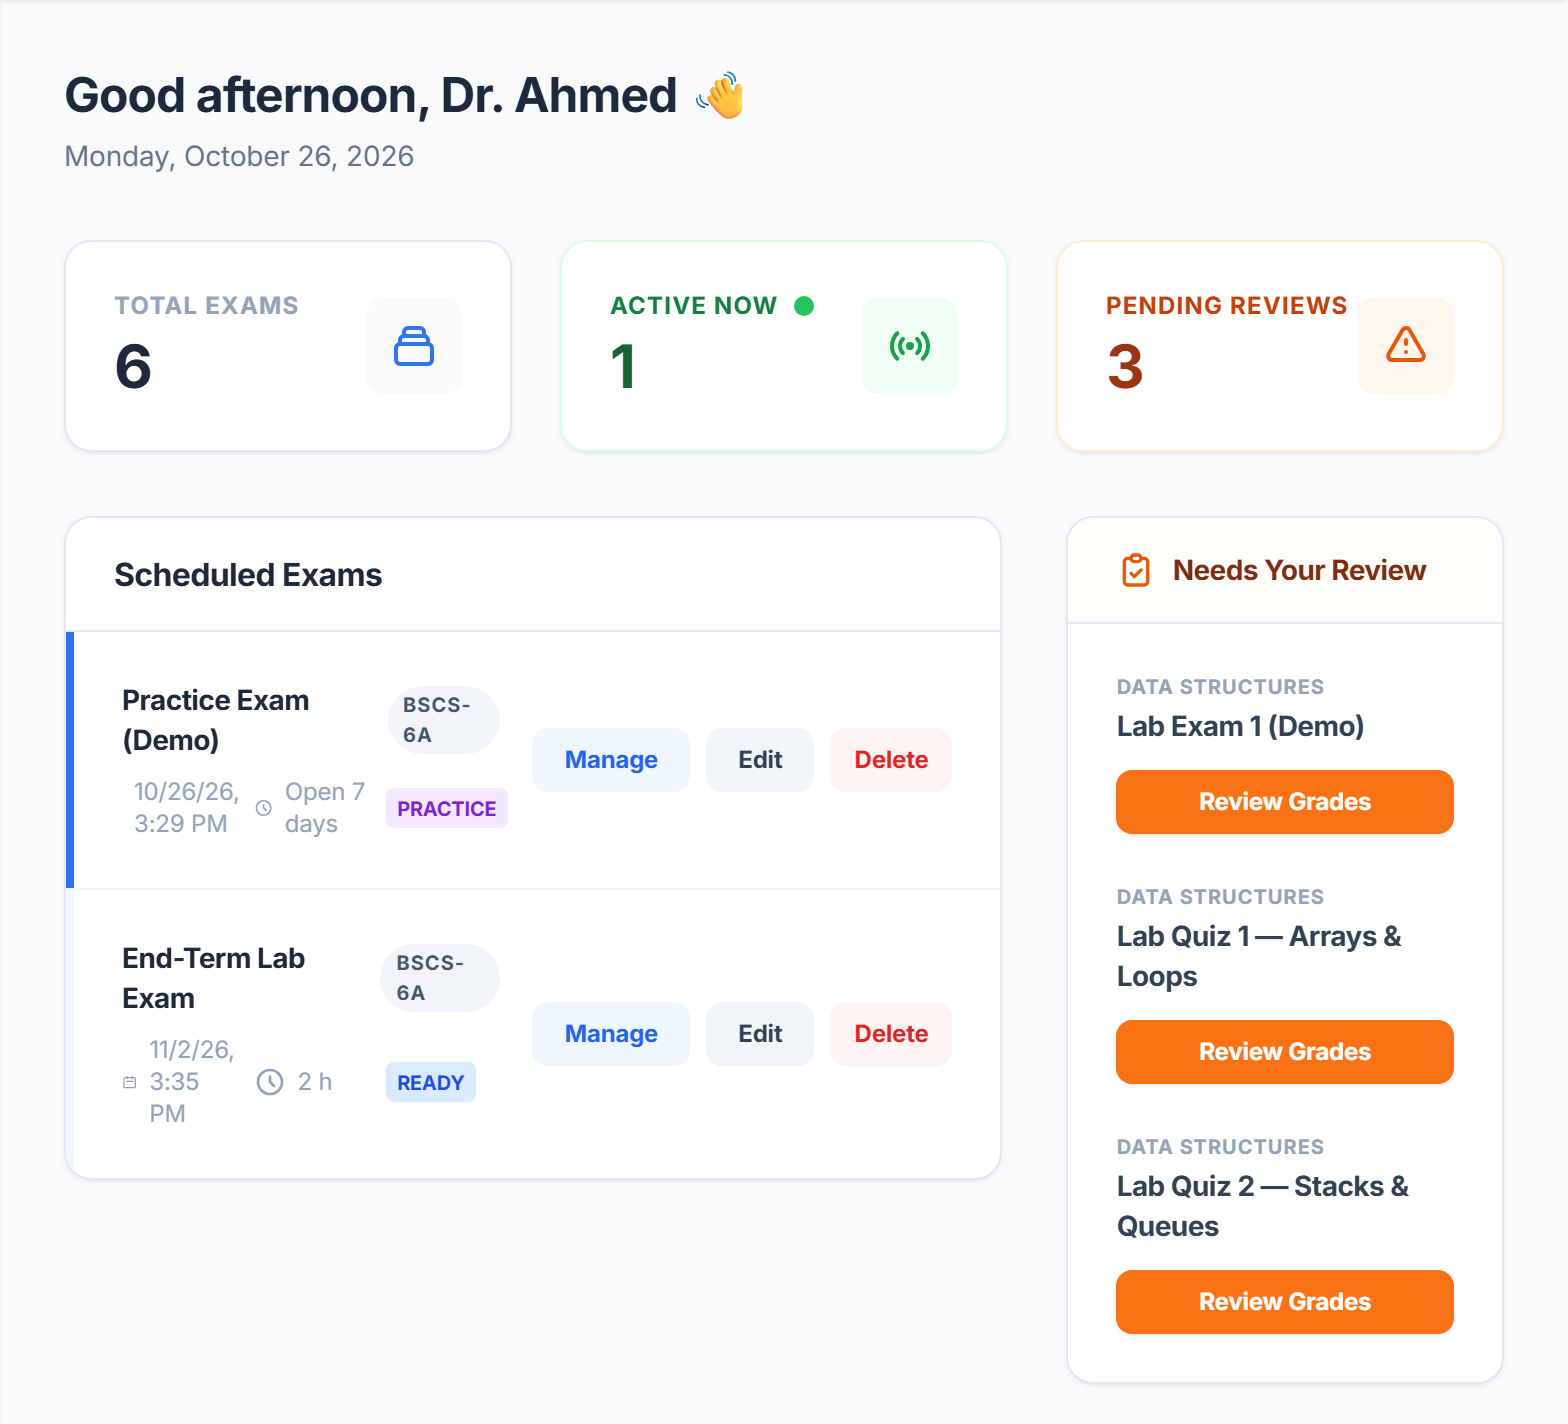
\includegraphics[width=\linewidth,height=410pt,keepaspectratio]{Figures/ui_teacher_dashboard.png}
\caption{Teacher Dashboard}
\label{fig:ui_teacher_dashboard}
\end{figure}
\SoftBarrierN

\begin{figure}[p]
\centering
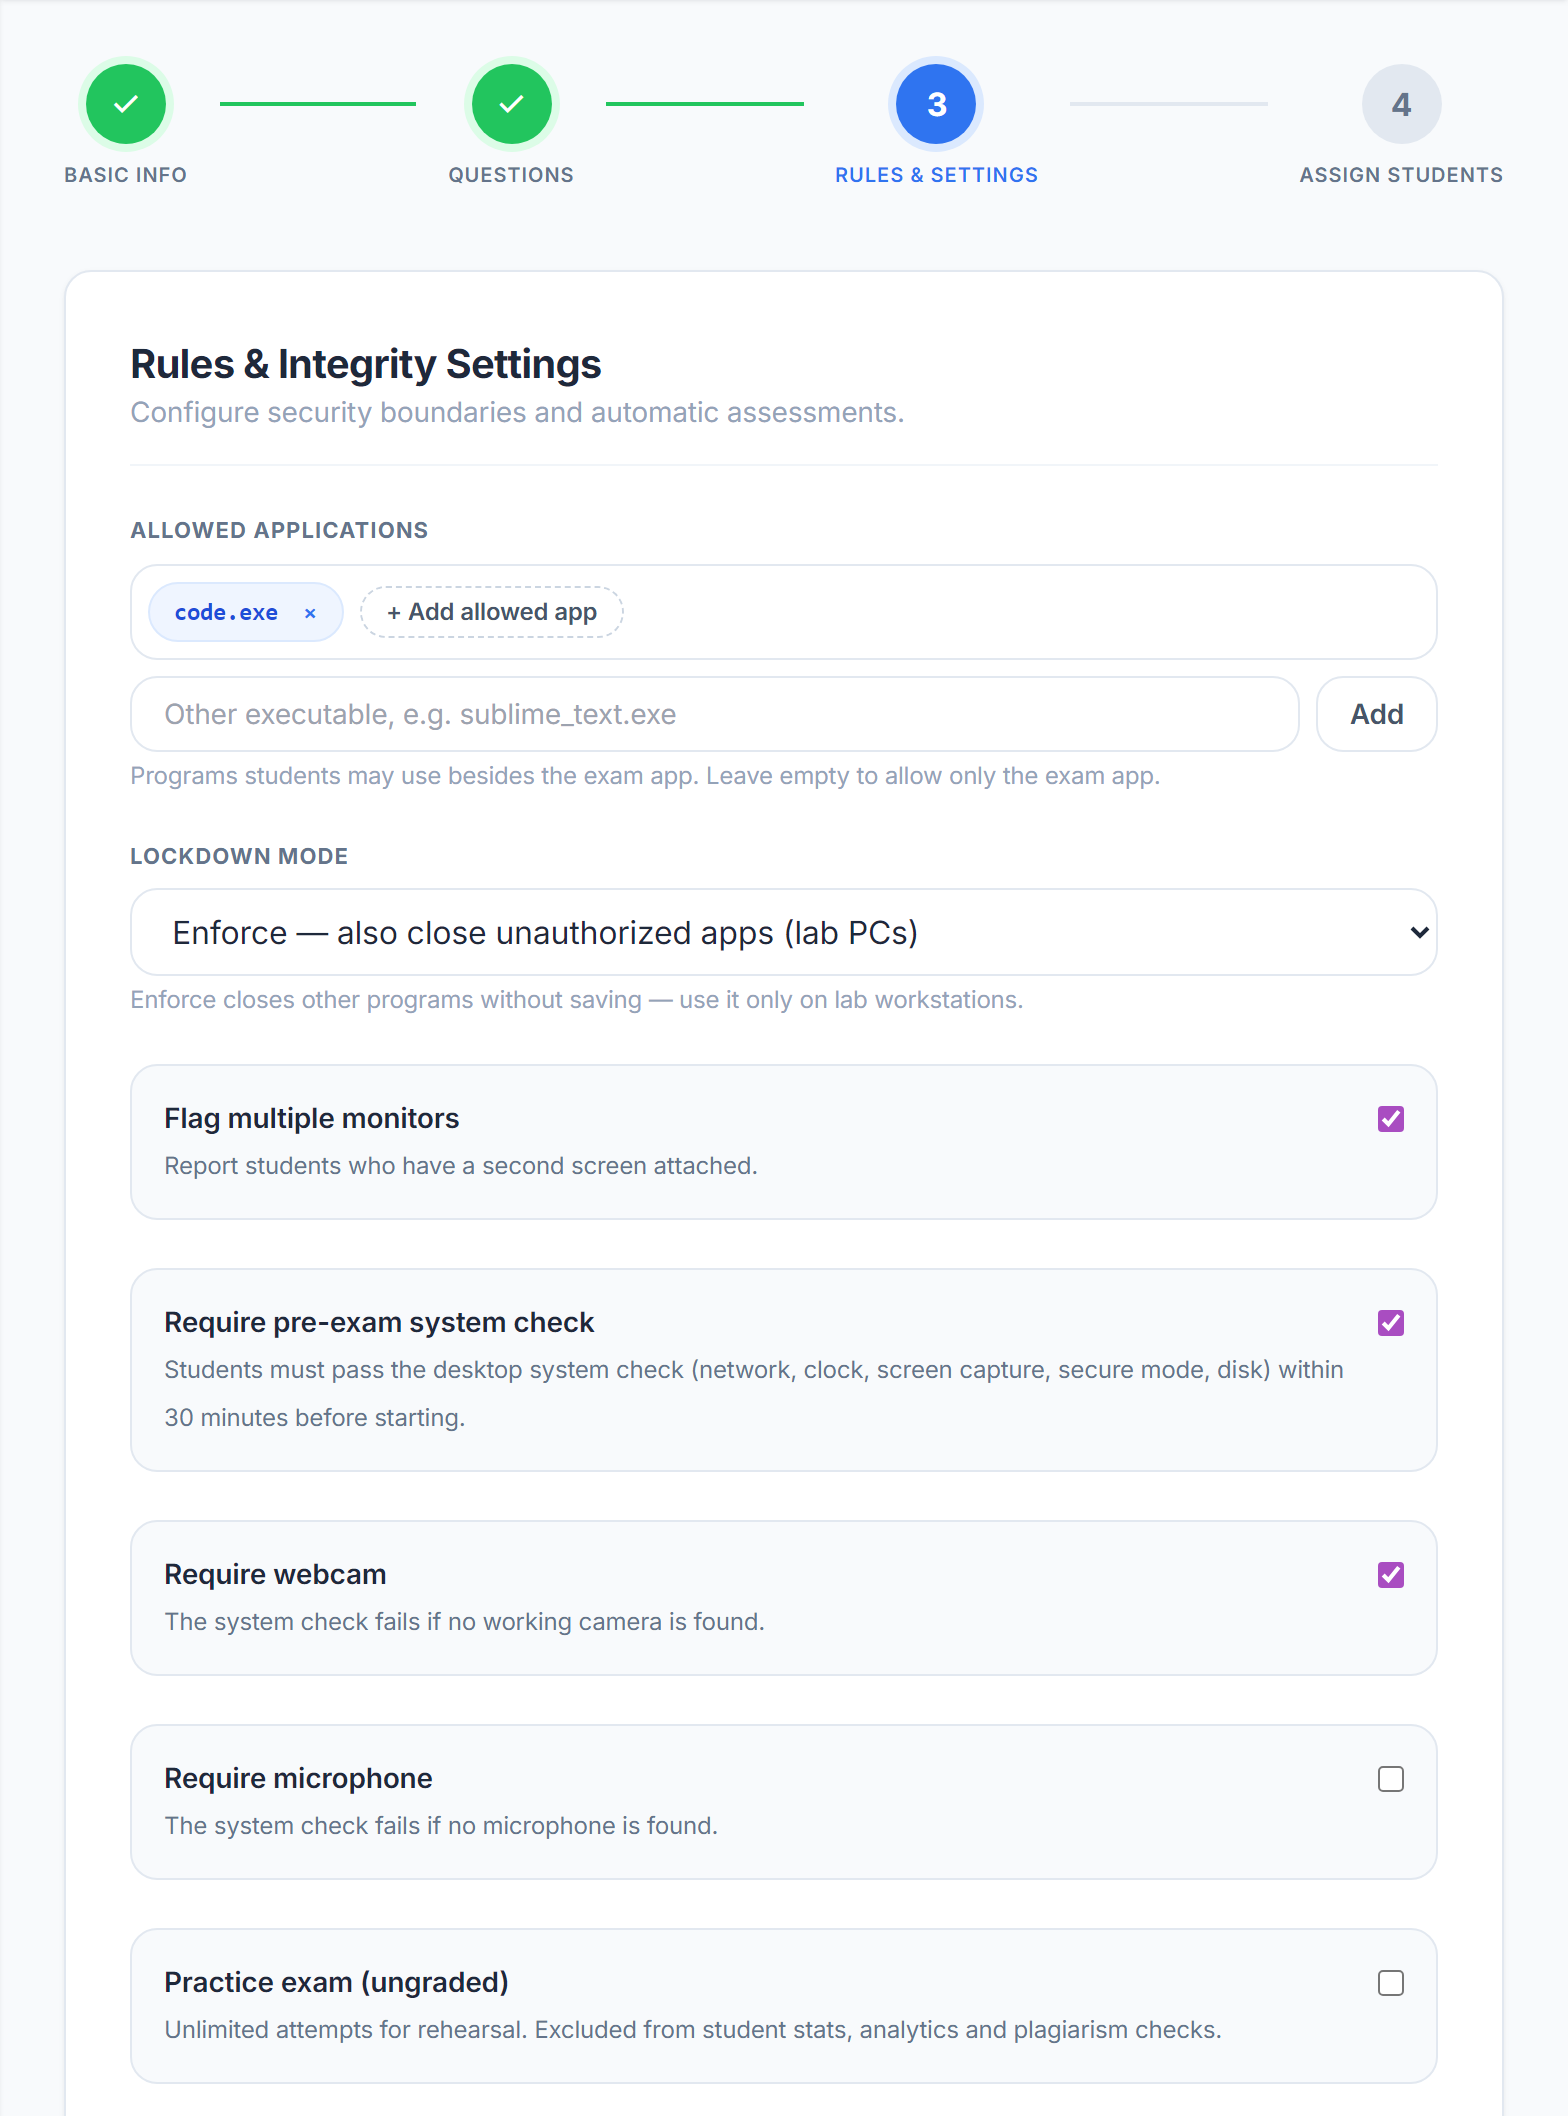
\includegraphics[width=\linewidth,height=628pt,keepaspectratio]{Figures/ui_create_exam_rules.png}
\caption{Create-Exam Wizard, Rules Step: Integrity Switches}
\label{fig:ui_create_exam_rules}
\end{figure}
\SoftBarrierN

A four-step wizard creates an exam: basic information, questions (MCQ, coding with test cases, theory), rules, and students (FR8). Step~3 holds the integrity rules: allowed applications, lockdown mode (Off, Report, Enforce), the multi-monitor flag, the required system check, webcam and microphone, and the practice-exam switch (Figure~\ref{fig:ui_create_exam_rules}); then early join, minimum attendance, the screenshot and webcam intervals, seat enforcement, AI evaluation and the plagiarism threshold (Figure~\ref{fig:ui_create_exam_rules_more}).

In Figure~\ref{fig:ui_create_exam_rules} the step bar shows that \emph{Basic Info} and \emph{Questions} are done and \emph{Rules \& Settings} is the current step. In this example only \texttt{code.exe} is allowed, and the lockdown mode is Enforce, which closes other programs without saving, so the hint says to use it only on lab PCs. The multi-monitor flag, the system check and the webcam are switched on, while the microphone and the practice-exam switch are off.

Figure~\ref{fig:ui_create_exam_rules_more} shows the lower half of the same step. Here early join is 0 minutes, the minimum attendance is 75\,\%, both capture intervals are 60~s, seat enforcement and AI evaluation are on, and the plagiarism threshold is 70\,\%. The hint under the screenshot interval explains that each gap is randomised by $\pm$50\,\% (30--90~s for 60~s) and that a violation causes an immediate capture, so a student cannot predict when the next capture comes.

\begin{figure}[tbp]
\centering
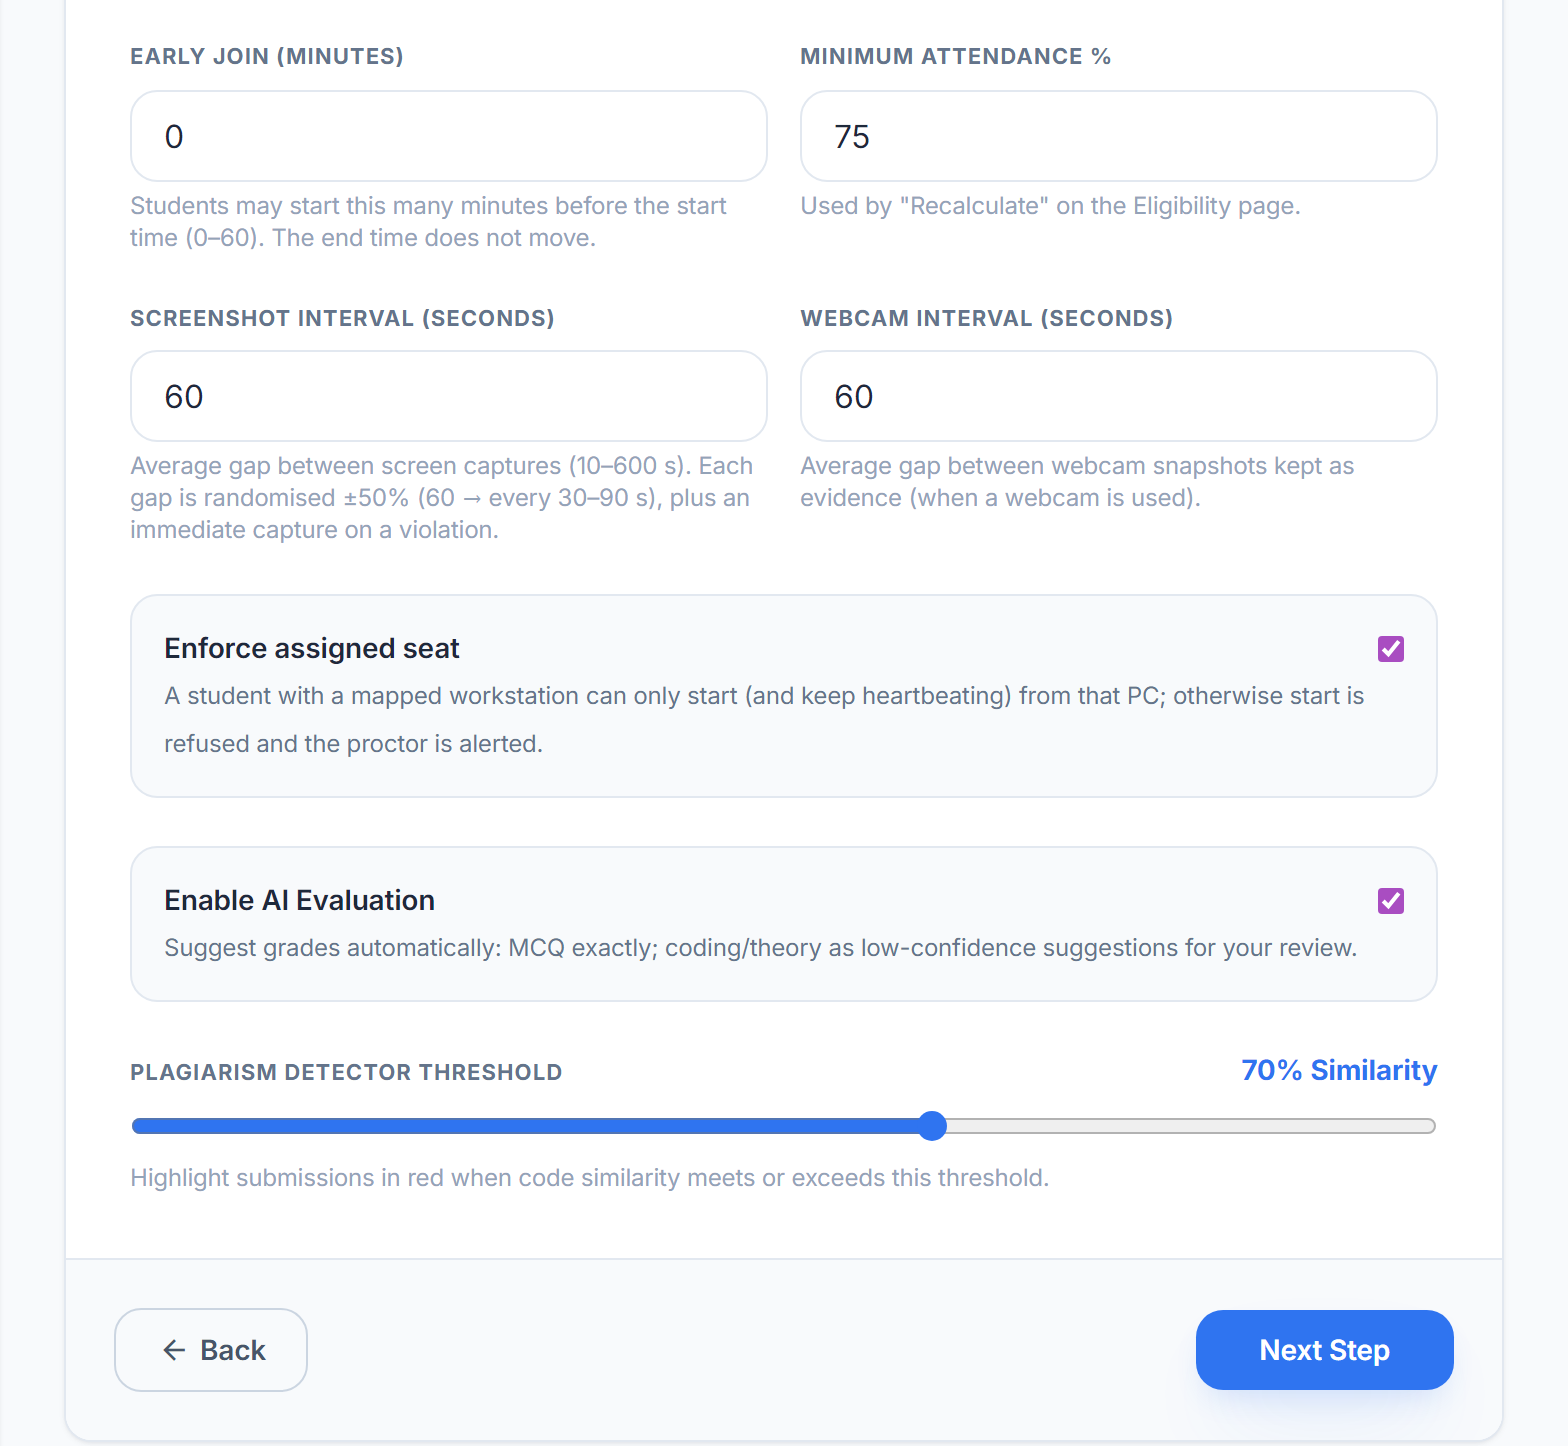
\includegraphics[width=\linewidth,height=416pt,keepaspectratio]{Figures/ui_create_exam_rules_more.png}
\caption{Create-Exam Wizard, Rules Step: Intervals, Seat, AI and Plagiarism Settings}
\label{fig:ui_create_exam_rules_more}
\end{figure}
\SoftBarrierN

On the eligibility page (Figure~\ref{fig:ui_eligibility}) the teacher uploads an attendance CSV (comma-separated values) file and clicks \emph{Recalculate}; students below the exam's minimum attendance become ineligible (FR9), as Hamza Iqbal (60\,\%) is here. Each row shows where its decision came from (\emph{Attendance} in the figure); a saved toggle for a single student becomes a \emph{Manual} override, which survives recalculation and is audited. The same page maps each student to a workstation (seat) and assigns invigilators, who then see only this exam.

The page is printed in two parts that show the same six rows in the same order. Part~(a) (Figure~\ref{fig:ui_eligibility}) holds the exam selector with its minimum attendance of 75\,\%, the \emph{Invigilators} card with Mr. Bilal assigned, and each student's name with a seat drop-down (R1C1 to R2C2 in Lab~A). Part~(b) (Figure~\ref{fig:ui_eligibility_b}) holds the buttons \emph{Upload Attendance}, \emph{Recalculate}, \emph{Mark All Eligible} and \emph{Mark All Ineligible}, the invigilator picker, and for each row the system check, the attendance, the eligibility switch with its source tag and the reason. Five students have 77.5--95\,\% attendance and are eligible. The last row is Hamza Iqbal: with 60\,\% (24 of 40 classes) his switch is off and the reason \emph{Attendance 60\% < 75\%} is shown in red. A green tick in the system-check column means a passing check less than 30 minutes old; Hamza has a dash because no check is recorded for him.

\begin{figure}[tbp]
\centering
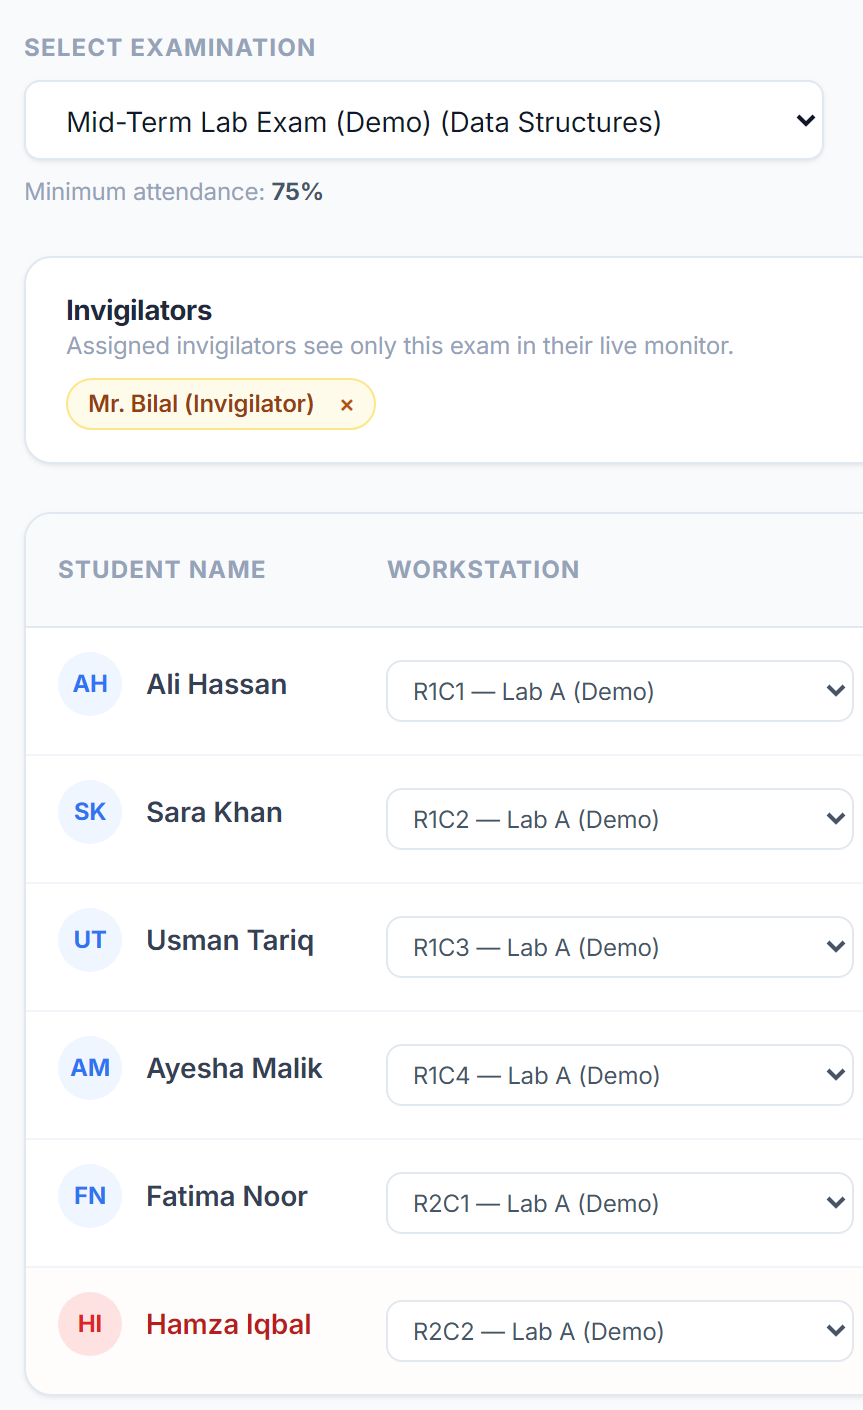
\includegraphics[width=0.72\linewidth]{Figures/ui_eligibility_p1.png}
\caption{Eligibility, Seats and Invigilators (a): Exam, Invigilators and Seats (Email Column Omitted)}
\label{fig:ui_eligibility}
\end{figure}
\SoftBarrierN

\begin{figure}[tbp]
\centering
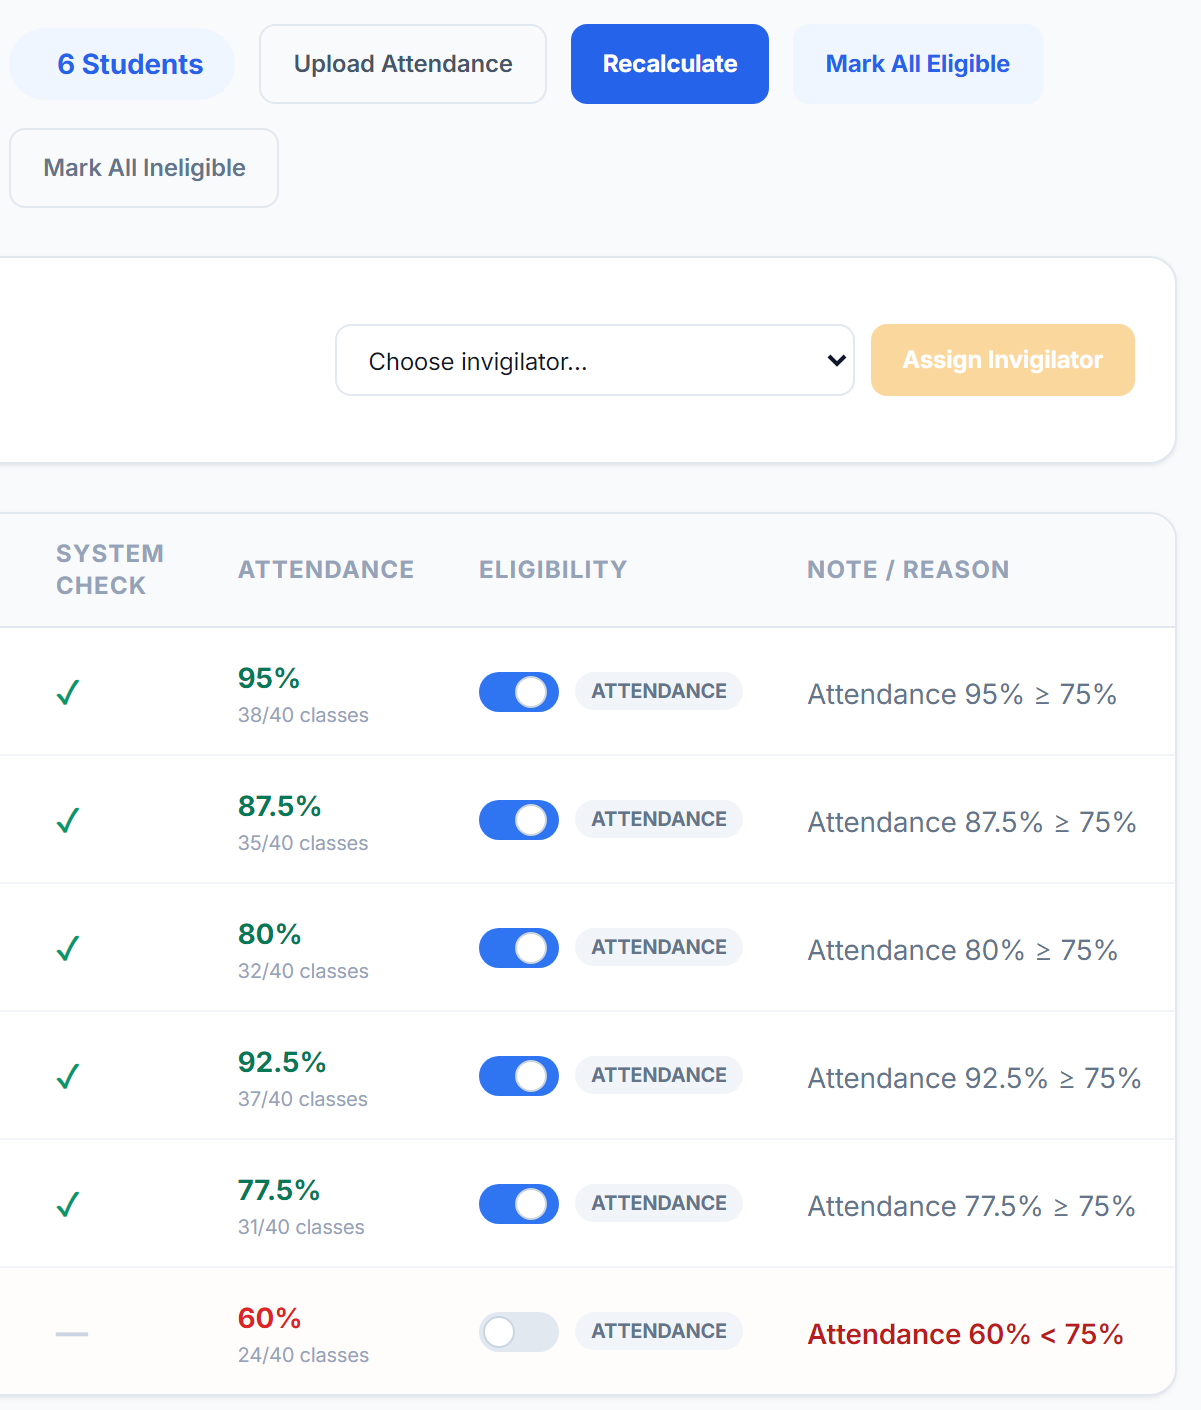
\includegraphics[width=\linewidth]{Figures/ui_eligibility_p2.png}
\caption{Eligibility, Seats and Invigilators (b): Attendance and Eligibility (Same Rows as Part (a))}
\label{fig:ui_eligibility_b}
\end{figure}
\SoftBarrierN

\subsection{Live Invigilation}\suppressfloats[t]
SignalR carries live updates between the API and the web dashboard; the desktop client uses REST only and receives invigilator warnings, extra time, unlocks and force-submits in the reply to its next heartbeat (every 10~s). The client sends heartbeats, event batches and screen captures to \url{/api/monitoring}, and the server pushes each update to the live monitor (Figures~\ref{fig:ui_teacher_live_monitoring} to~\ref{fig:ui_teacher_live_monitoring_b}) over the hub \url{/hubs/monitoring} (FR5, FR10). Through \texttt{ExamProctors}, invigilators see only the exams assigned to them. The header of the live monitor (Figure~\ref{fig:ui_teacher_live_monitoring}) names the current exam with its course tag and an exam selector, and shows the remaining time (01:27:10) on the right. It also shows that four students are still sitting (Ali Hassan has already submitted) and gives the \emph{Extend Time} and \emph{Force End Exam} buttons, which act on the whole exam.

\begin{figure}[tbp]
\centering
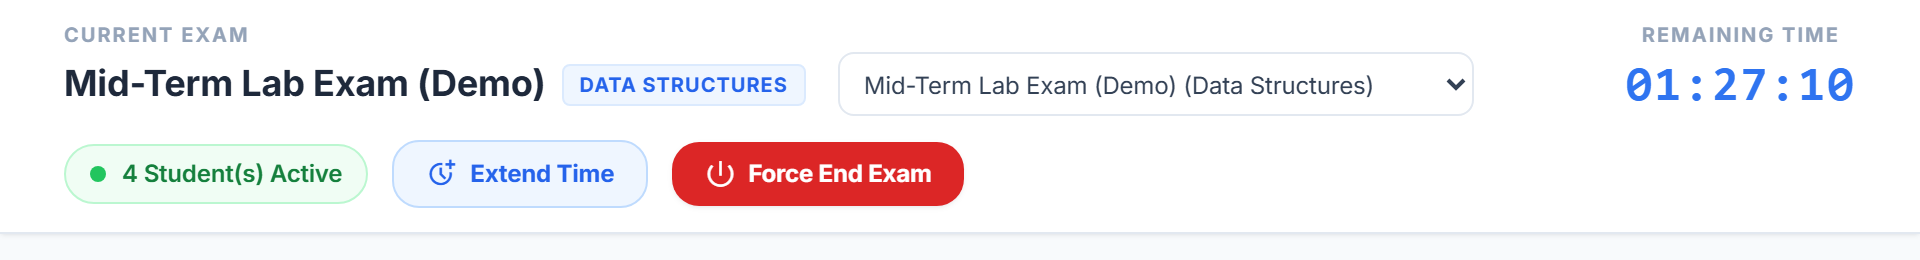
\includegraphics[width=\linewidth]{Figures/ui_live_monitor_a_p1.png}
\caption{Live Monitor (a): Header with Remaining Time and Exam Controls}
\label{fig:ui_teacher_live_monitoring}
\end{figure}
\SoftBarrierN

Below the header each student has a tile (Figures~\ref{fig:ui_teacher_live_monitoring_tiles} to~\ref{fig:ui_teacher_live_monitoring_b}). Each tile shows the student's seat and PC with the Windows user, readiness, latest capture, latest alert and progress as answered questions with a bar. The heart icon and the border colour give the status: the classifier level as Stable (Normal), Warning, Suspicious or Critical (Violation); a client silent for 30~s is shown as Disconnected, and a finished session as Submitted, Force submitted or Timed out. The captures are small thumbnails, and their text is not meant to be read at this size.

Ali Hassan (seat R1C1) has answered all three questions and submitted, and Sara Khan (R1C2) is a Warning with one alert, \emph{Blocked keys}, for her blocked Alt+Tab (Figure~\ref{fig:ui_teacher_live_monitoring_tiles}). Usman Tariq (R1C3) is Critical with two alerts and one incident (Figure~\ref{fig:ui_teacher_live_monitoring_tile3}): he opened Chrome, which is not on the allowed list, and Enforce mode closed it, as the line \emph{Unauthorized app closed: chrome (Killed)} says; his capture shows a browser search. In the second row (Figure~\ref{fig:ui_teacher_live_monitoring_b}), Ayesha Malik's phone in view makes her Suspicious, and Fatima Noor is Stable with an \emph{Idle 9m} badge, which means no keyboard or mouse input on her PC for nine minutes.

\begin{figure}[tbp]
\centering
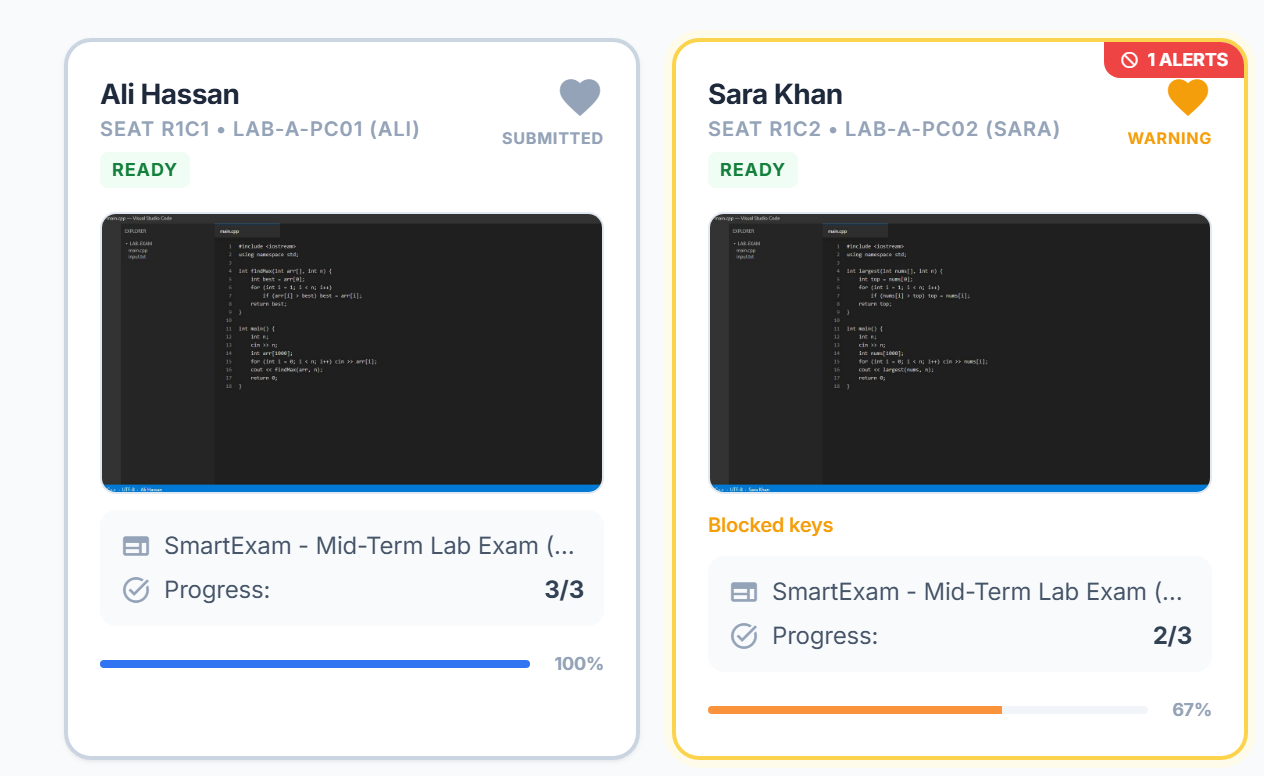
\includegraphics[width=\linewidth]{Figures/ui_live_monitor_a_p2.png}
\caption{Live Monitor (b): First Row, Tiles of Ali Hassan and Sara Khan}
\label{fig:ui_teacher_live_monitoring_tiles}
\end{figure}
\SoftBarrierN

\begin{figure}[tbp]
\centering
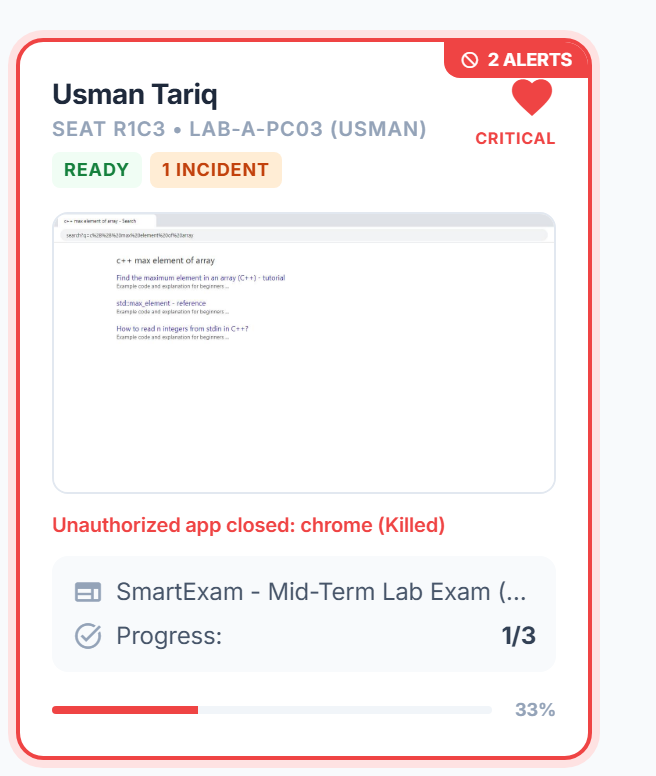
\includegraphics[width=0.52\linewidth]{Figures/ui_live_monitor_a_p3.png}
\caption{Live Monitor (c): First Row, Tile of Usman Tariq}
\label{fig:ui_teacher_live_monitoring_tile3}
\end{figure}
\SoftBarrierN

\begin{figure}[tbp]
\centering
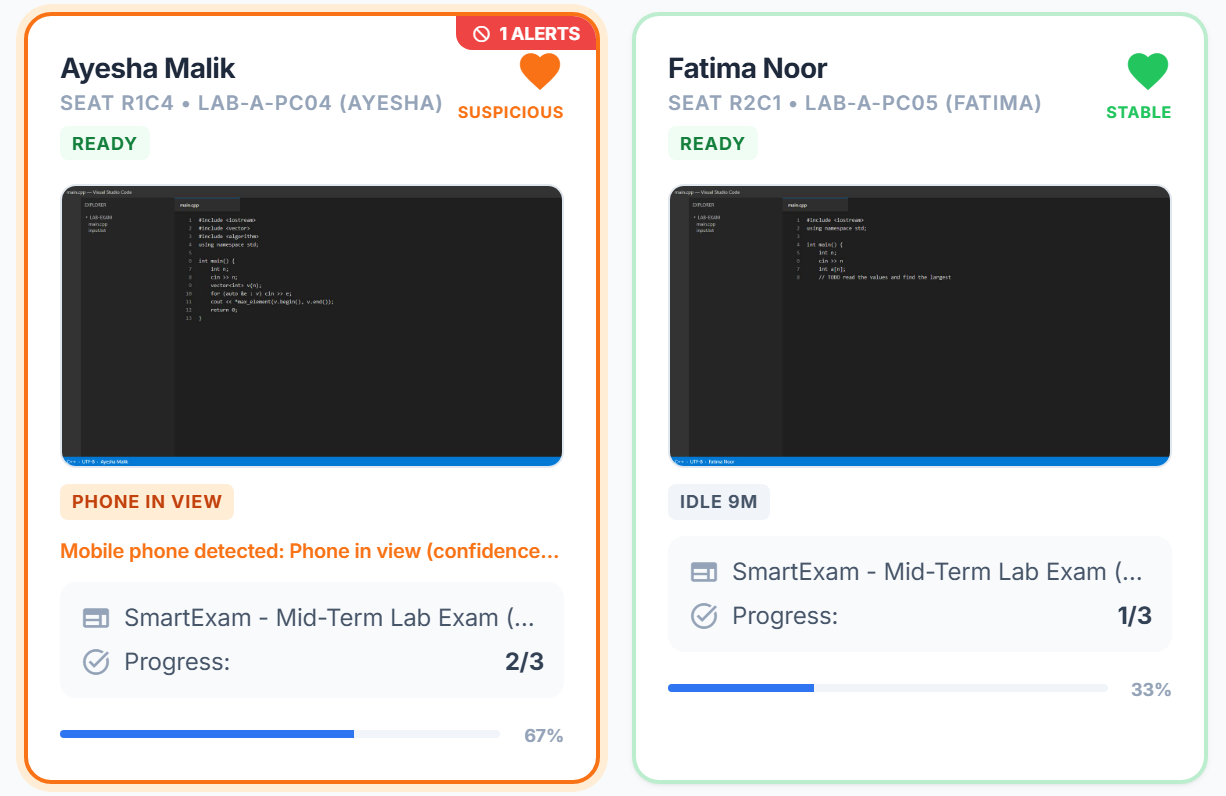
\includegraphics[width=\linewidth,height=293pt,keepaspectratio]{Figures/ui_live_monitor_b.png}
\caption{Live Monitor (d): Second Row of Tiles}
\label{fig:ui_teacher_live_monitoring_b}
\end{figure}
\SoftBarrierN

Clicking a tile opens the student drawer, here for Usman Tariq (Figure~\ref{fig:ui_live_drawer}). Its top gives the seat, the PC and the Windows user with the number of active alerts and open incidents. Below are the latest captures (the newer one, outlined in orange, shows the browser search), the readiness result (all seven checks passed on LAB-A-PC03 at 3:35:26~PM) and the applications seen on the PC, where Chrome is struck through because it is no longer running. So the invigilator sees all the evidence for one student in one place before acting.

\begin{figure}[p]
\centering
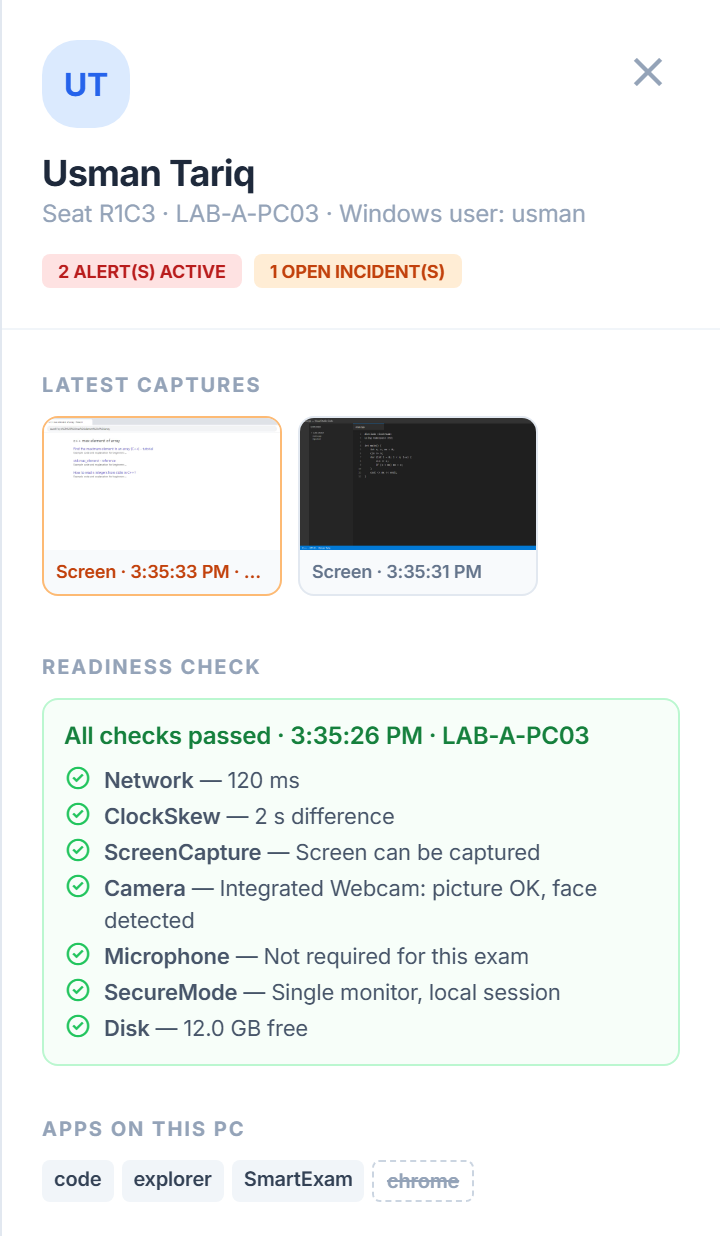
\includegraphics[width=\linewidth,height=628pt,keepaspectratio]{Figures/ui_live_drawer_evidence.png}
\caption{Student Drawer (a): Evidence}
\label{fig:ui_live_drawer}
\end{figure}
\SoftBarrierN

From the action panel (Figure~\ref{fig:ui_live_drawer_b}) the invigilator sends a warning, records an incident, unlocks the PC for five minutes with a short reason (the server allows 1--30 minutes), grants extra time or force-submits the session (FR10). The green line \emph{Warning Message Sent} confirms that the warning was sent. Force-submit is the red button because it ends the student's attempt; like the other actions, it reaches the desktop client in the reply to its next heartbeat.

\begin{figure}[tbp]
\centering
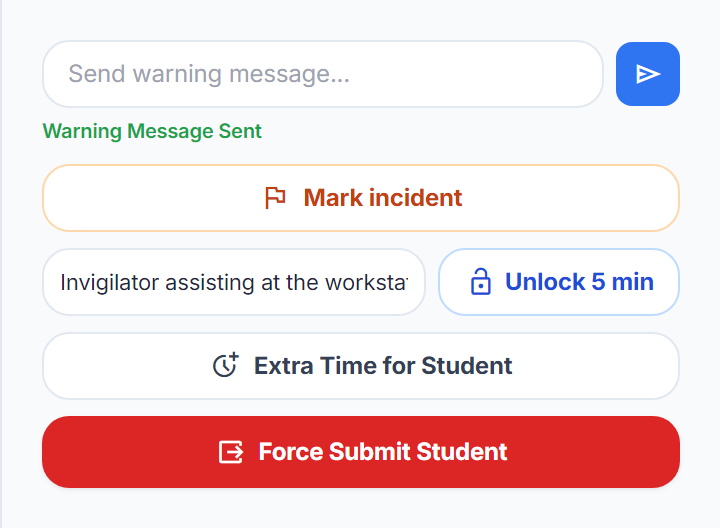
\includegraphics[width=0.55\linewidth]{Figures/ui_live_drawer_actions.png}
\caption{Student Drawer (b): Actions}
\label{fig:ui_live_drawer_b}
\end{figure}
\SoftBarrierN

Further down (Figure~\ref{fig:ui_live_timeline}) are the open incidents, with \emph{Escalate} and \emph{Mark resolved}, and the activity timeline. The incident card shows its severity (High), its status (Open), the note and who recorded it (Dr. Ahmed). The timeline lists the events newest first: Chrome closed by Enforce mode at 3:35:33~PM, the incident recorded at the same time, and the warning sent ten seconds later, which is the banner of Figure~\ref{fig:ui_student_warning}.

\begin{figure}[tbp]
\centering
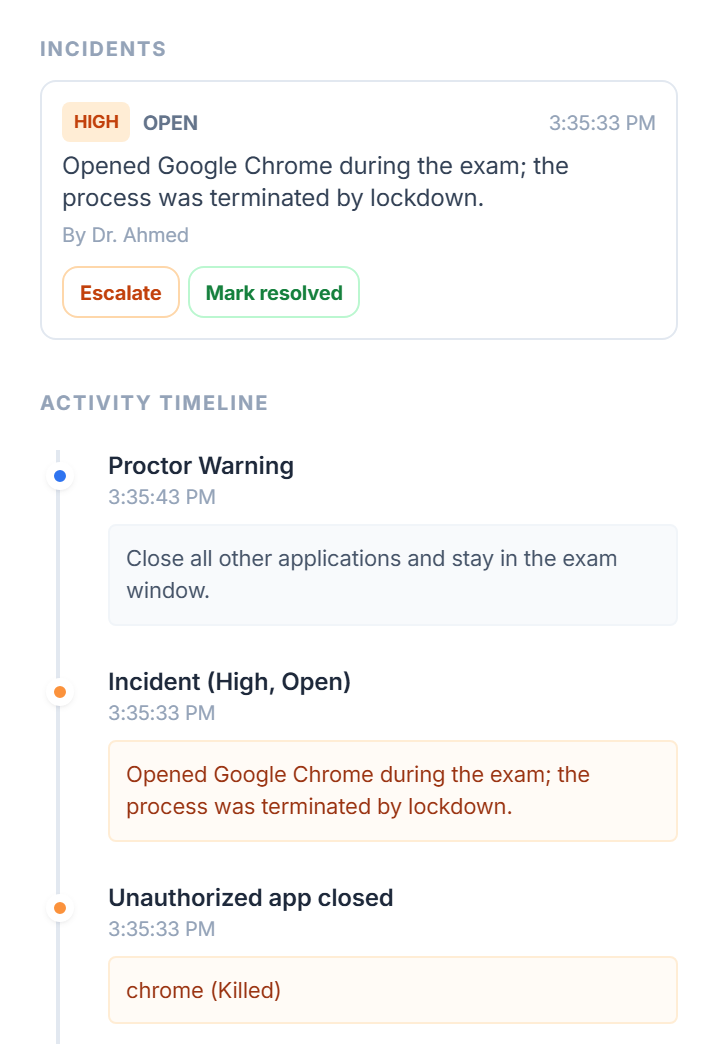
\includegraphics[width=0.60\linewidth,height=418pt,keepaspectratio]{Figures/ui_live_timeline.png}
\caption{Student Drawer (c): Incident and Activity Timeline}
\label{fig:ui_live_timeline}
\end{figure}
\SoftBarrierN

\subsection{Evaluation}\suppressfloats[t]
The results page lists each submission with its score and SHA-256 receipt. Opening one (Figures~\ref{fig:ui_teacher_ai_grading} and~\ref{fig:ui_teacher_ai_grading_b}) shows every answer next to its AI evaluation: suggested mark, confidence, engine, justification, test-case results (hidden cases marked) and code-analysis signals. Coding answers (C or C++ only) are compiled and run against weighted test cases \cite{alamutka2005} in an isolated Docker \texttt{gcc:13} container when Docker is available; otherwise a local MinGW g++ runner, which is not isolated, is used, and with no runner the answer is left for teacher review (FR11.1). Theory answers get a TF-IDF similarity score \cite{salton1988} (FR11.2). The teacher accepts the mark or saves an override, stored in \texttt{TeacherGradeOverrides}.

Figure~\ref{fig:ui_teacher_ai_grading} shows the top of the review for Usman Tariq: his status (Submitted), the question with its type and maximum (Coding, 20 marks) and his submitted code. His program starts the maximum at 0 instead of at the first element, so it prints a wrong answer when all the numbers are negative. The evaluation card below shows how the grader finds this mistake.

\begin{figure}[tbp]
\centering
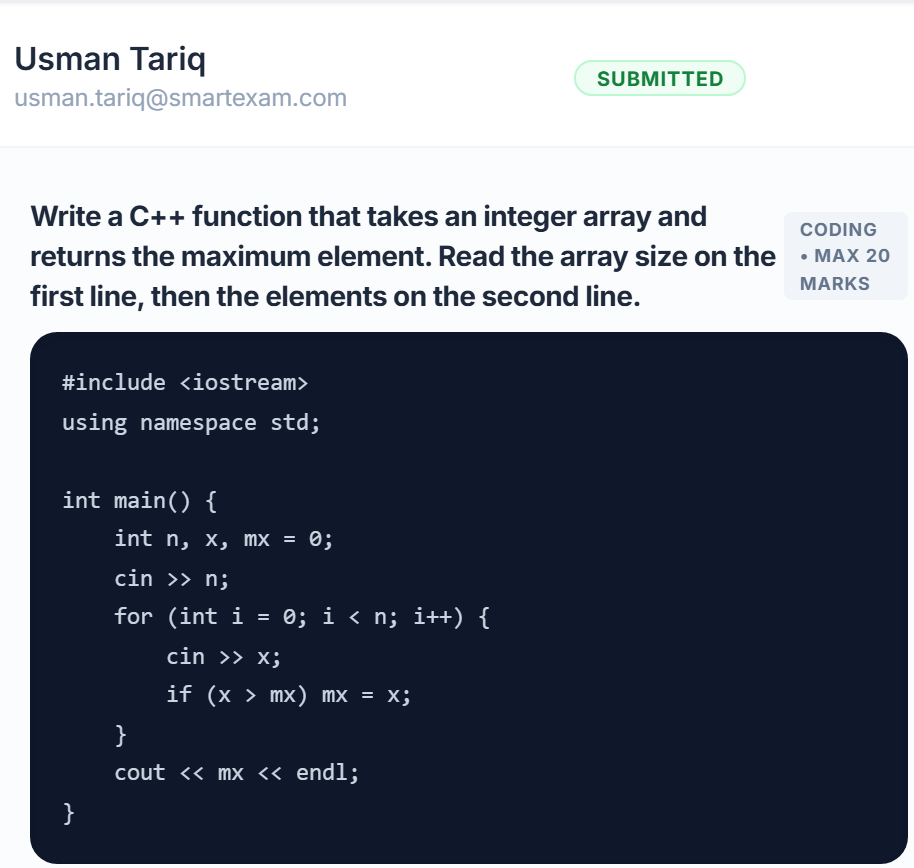
\includegraphics[width=0.85\linewidth,height=370pt,keepaspectratio]{Figures/ui_ai_grading_answer.png}
\caption{AI Evaluation of a Coding Answer (a): Question and Submitted Code}
\label{fig:ui_teacher_ai_grading}
\end{figure}
\SoftBarrierN

The AI evaluation card (Figure~\ref{fig:ui_teacher_ai_grading_b}) suggests 10 of 20 marks with medium confidence, from the isolated Docker engine. The test-case table explains the mark: the visible case passes, but the hidden case with the input $-1$, $-5$, $-2$ expects $-1$ and gets 0, so one of the two cases passes and half the marks are suggested. The code-analysis signals give O($n$) complexity, one loop and a medium hard-coding suspicion, because the code passes every visible case but fails a hidden one. The teacher can accept the 10 marks or enter another mark with a note and click \emph{Save Grade Override}.

\begin{figure}[tbp]
\centering
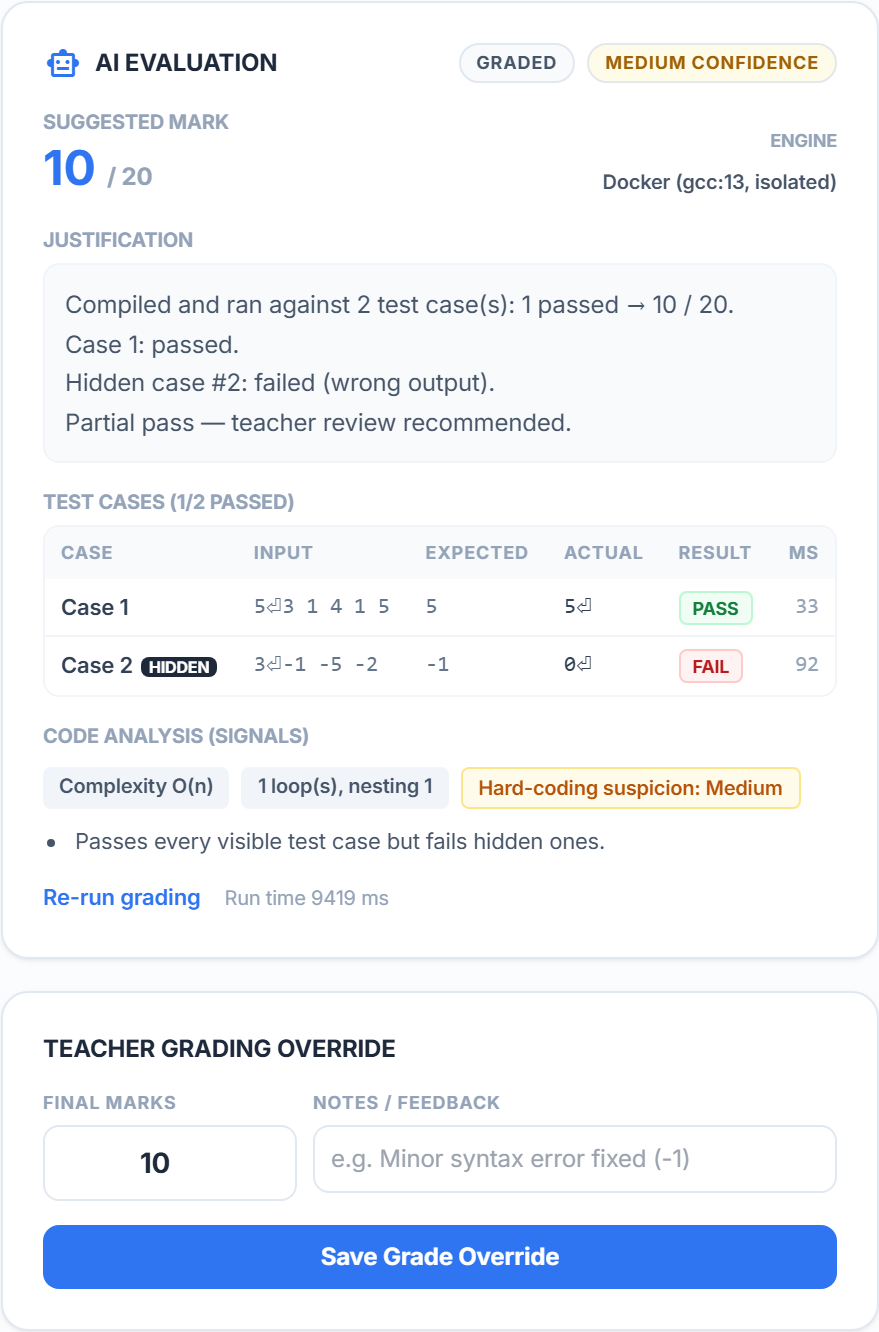
\includegraphics[width=\linewidth,height=565pt,keepaspectratio]{Figures/ui_ai_grading_eval.png}
\caption{AI Evaluation of a Coding Answer (b): Suggested Mark, Test Cases and Override}
\label{fig:ui_teacher_ai_grading_b}
\end{figure}
\SoftBarrierN

The \emph{Plagiarism Flags} tab (Figure~\ref{fig:ui_plagiarism}) shows a pairwise heat map built by k-gram winnowing \cite{winnowing}, which ignores identifiers and comments in code (FR11.3). A pair at or above the exam's threshold gets a card with both answers side by side and the matched lines highlighted; here Sara's program is Ali's with renamed variables. The teacher records the decision as a grade override.

In the heat map each row and column is a student (the columns use initials), and each cell is the highest similarity of that pair over all questions; darker cells are more similar, in 20\,\% steps. Only Ali Hassan and Sara Khan reach the 70\,\% threshold, at 100\,\%, while every other pair is at 25\,\% or below. The card below shows why: only the names differ (\texttt{largest}, \texttt{nums}, \texttt{top} against \texttt{findMax}, \texttt{arr}, \texttt{best}), so with identifiers ignored the code is the same. A note at the bottom reminds the teacher that similarity is evidence, not a verdict.

\begin{figure}[p]
\centering
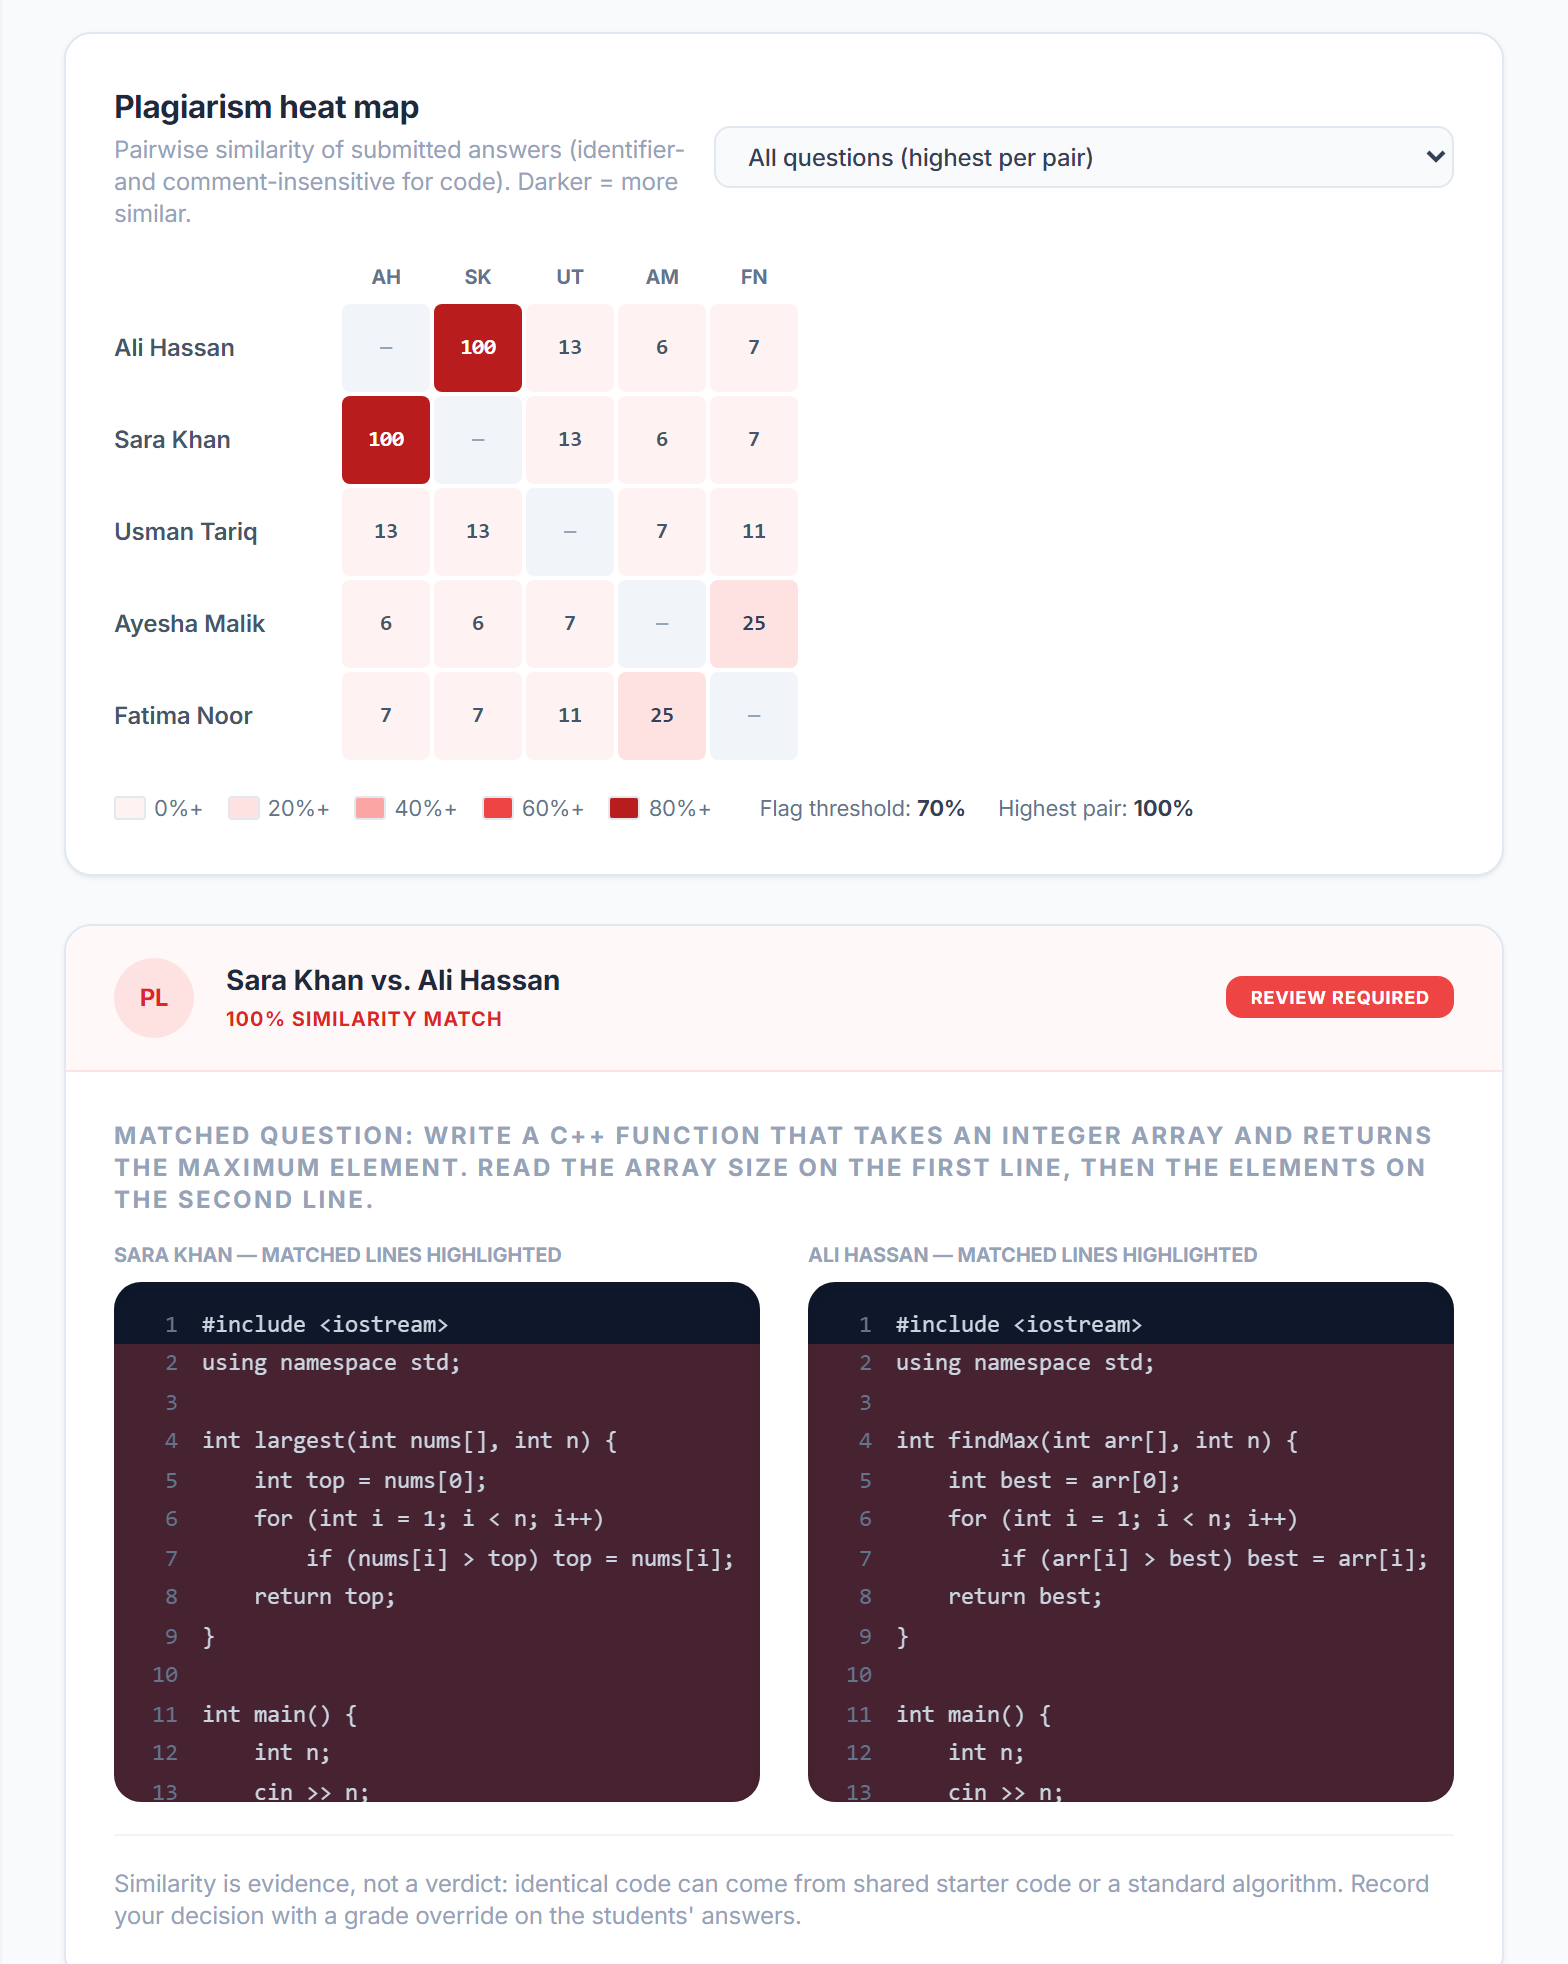
\includegraphics[width=\linewidth,height=562pt,keepaspectratio]{Figures/ui_plagiarism.png}
\caption{Plagiarism Heat Map and Matched Pair}
\label{fig:ui_plagiarism}
\end{figure}
\SoftBarrierN

\subsection{Administration and Student Portal}\suppressfloats[t]
Every web user, staff or student, signs in on one login page with email and password (Figure~\ref{fig:ui_web_login}) and is taken to the home page of their role. Neither front end offers self-registration or an emailed password reset: administrators create accounts or import them from a CSV file and can set a new password when editing an account (FR7), and staff change their own password from the panel (Figure~\ref{fig:seq_change_password}). The desktop client's sign-in and logout are drawn in Figures~\ref{fig:seq_login} and~\ref{fig:seq_logout}; on the web panel, sign-in, refresh and sign-out are tested in ST-01 (Table~\ref{tab:st_admin}). The figure shows the form filled in for the teacher account (\texttt{teacher@smartexam.com}), with an eye icon to show or hide the password. The note under \emph{Sign In} says that access attempts are logged, and this is true: the server writes every successful and failed login to the audit log (\texttt{LOGIN\_SUCCESS}, \texttt{LOGIN\_FAILED}).

\begin{figure}[htbp]
\centering
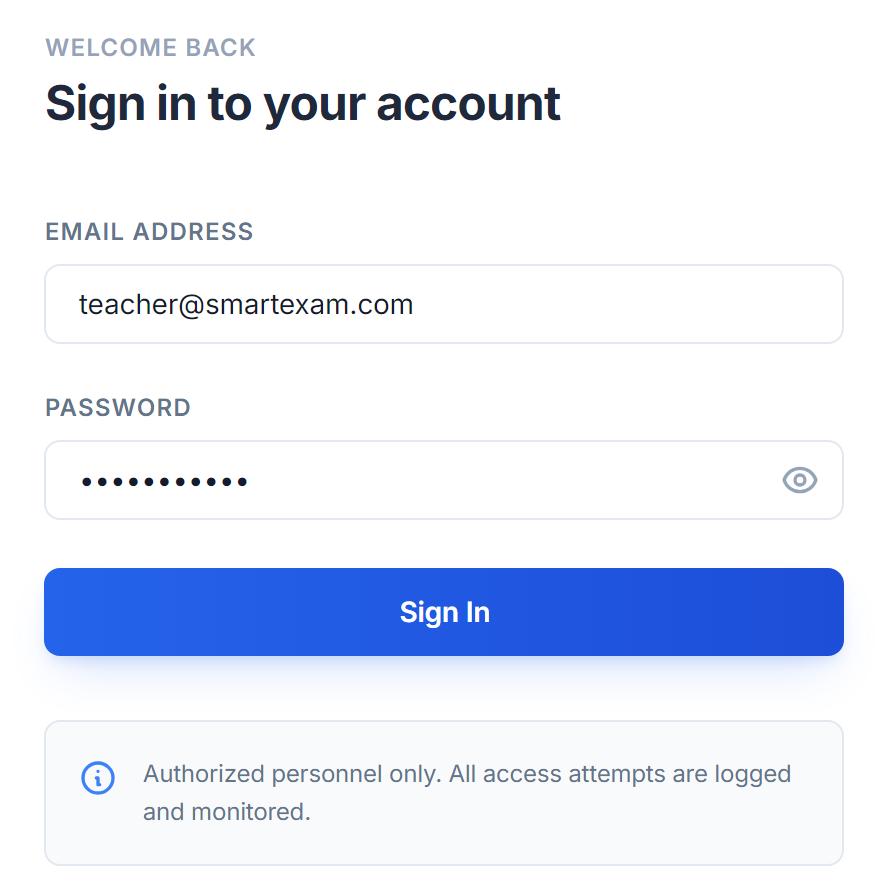
\includegraphics[width=0.62\linewidth]{Figures/ui_web_login.png}
\caption{Web Panel Login (Sign-In Form)}
\label{fig:ui_web_login}
\end{figure}
\SoftBarrierN

Admins manage departments and courses (Figure~\ref{fig:ui_academics}); department names are unique, a course code is unique within its department, and a department or course still in use cannot be deleted (FR7). The upper card lists the three departments with their number of courses (Computer Science 3, Electrical Engineering 1, Software Engineering 2). The lower card lists the six courses with code, name, department and number of sections, and can be filtered by department. Only CS301 Data Structures has a section, the one that owns the demo exams, so it is the only course here that cannot be deleted.

\begin{figure}[tbp]
\centering
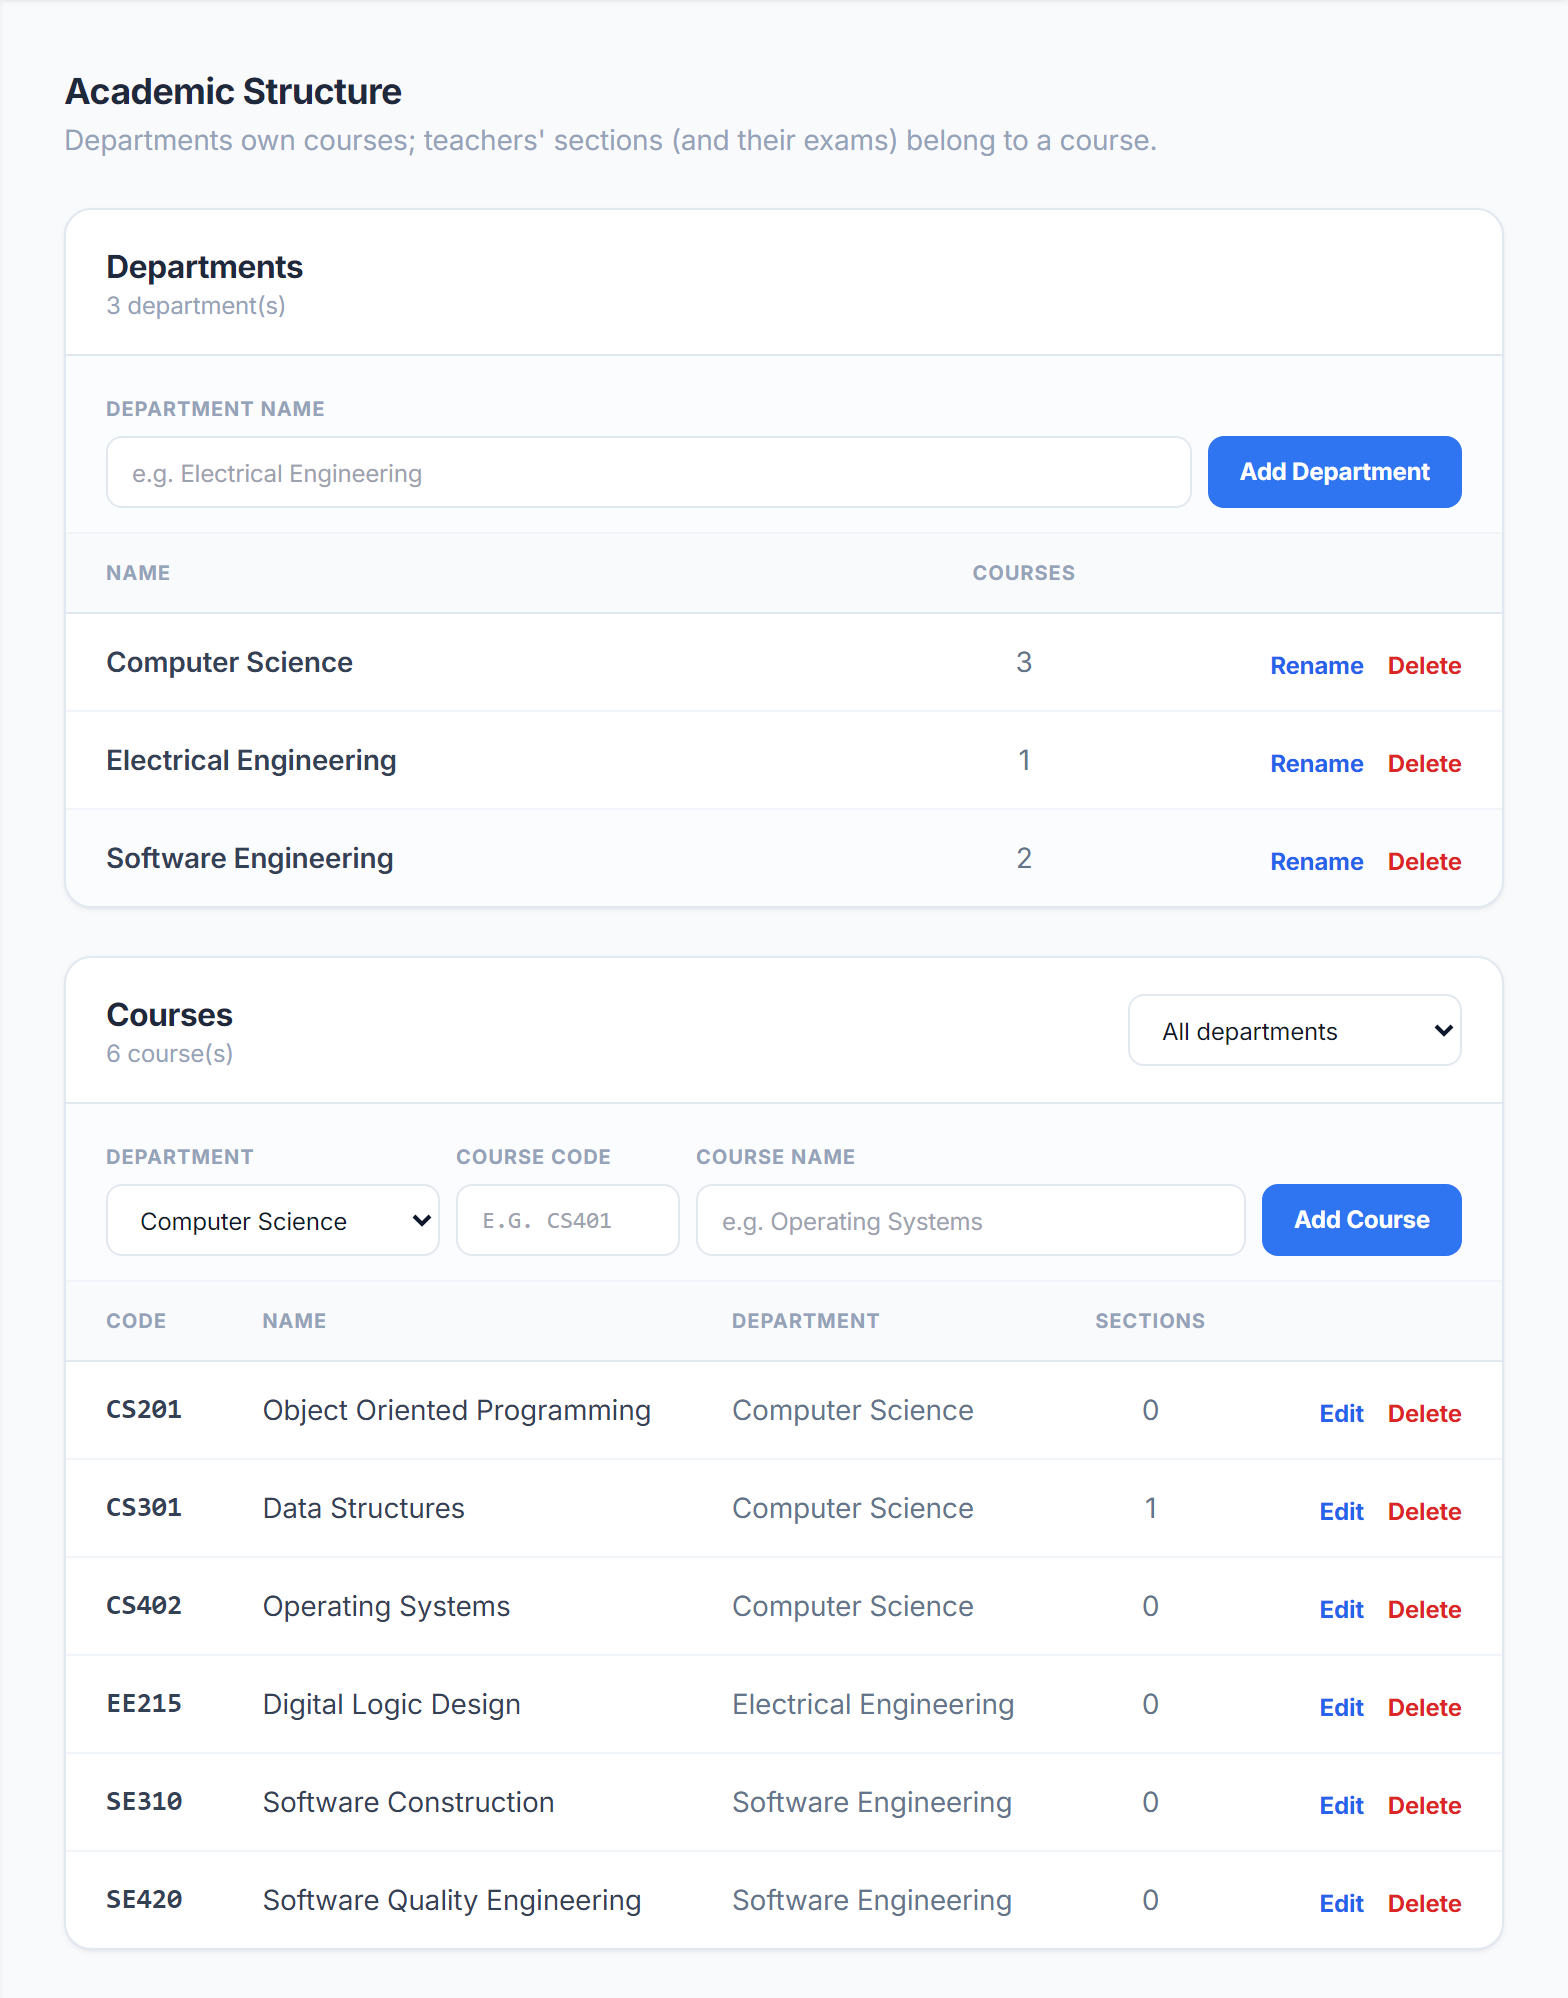
\includegraphics[width=\linewidth,height=600pt,keepaspectratio]{Figures/ui_academics.png}
\caption{Departments and Courses}
\label{fig:ui_academics}
\end{figure}
\SoftBarrierN

Admins register labs and workstations (machine number, Windows PC name, IP address) in Figure~\ref{fig:ui_labs_workstations}; each seat shows the student signed in on it. With \texttt{EnforceSeat} on, a student with a seat can start the exam only from that PC (FR9). The figure shows Lab~A (Demo) in Block~3, Ground Floor, with six workstations; each card gives the seat name, the IP address and the PC name. A green \emph{In use} card also shows the signed-in student, the Windows user and when the PC was last seen. R2C2 is \emph{Free} because Hamza Iqbal, who is seated there, is not eligible and has not signed in.

\begin{figure}[tbp]
\centering
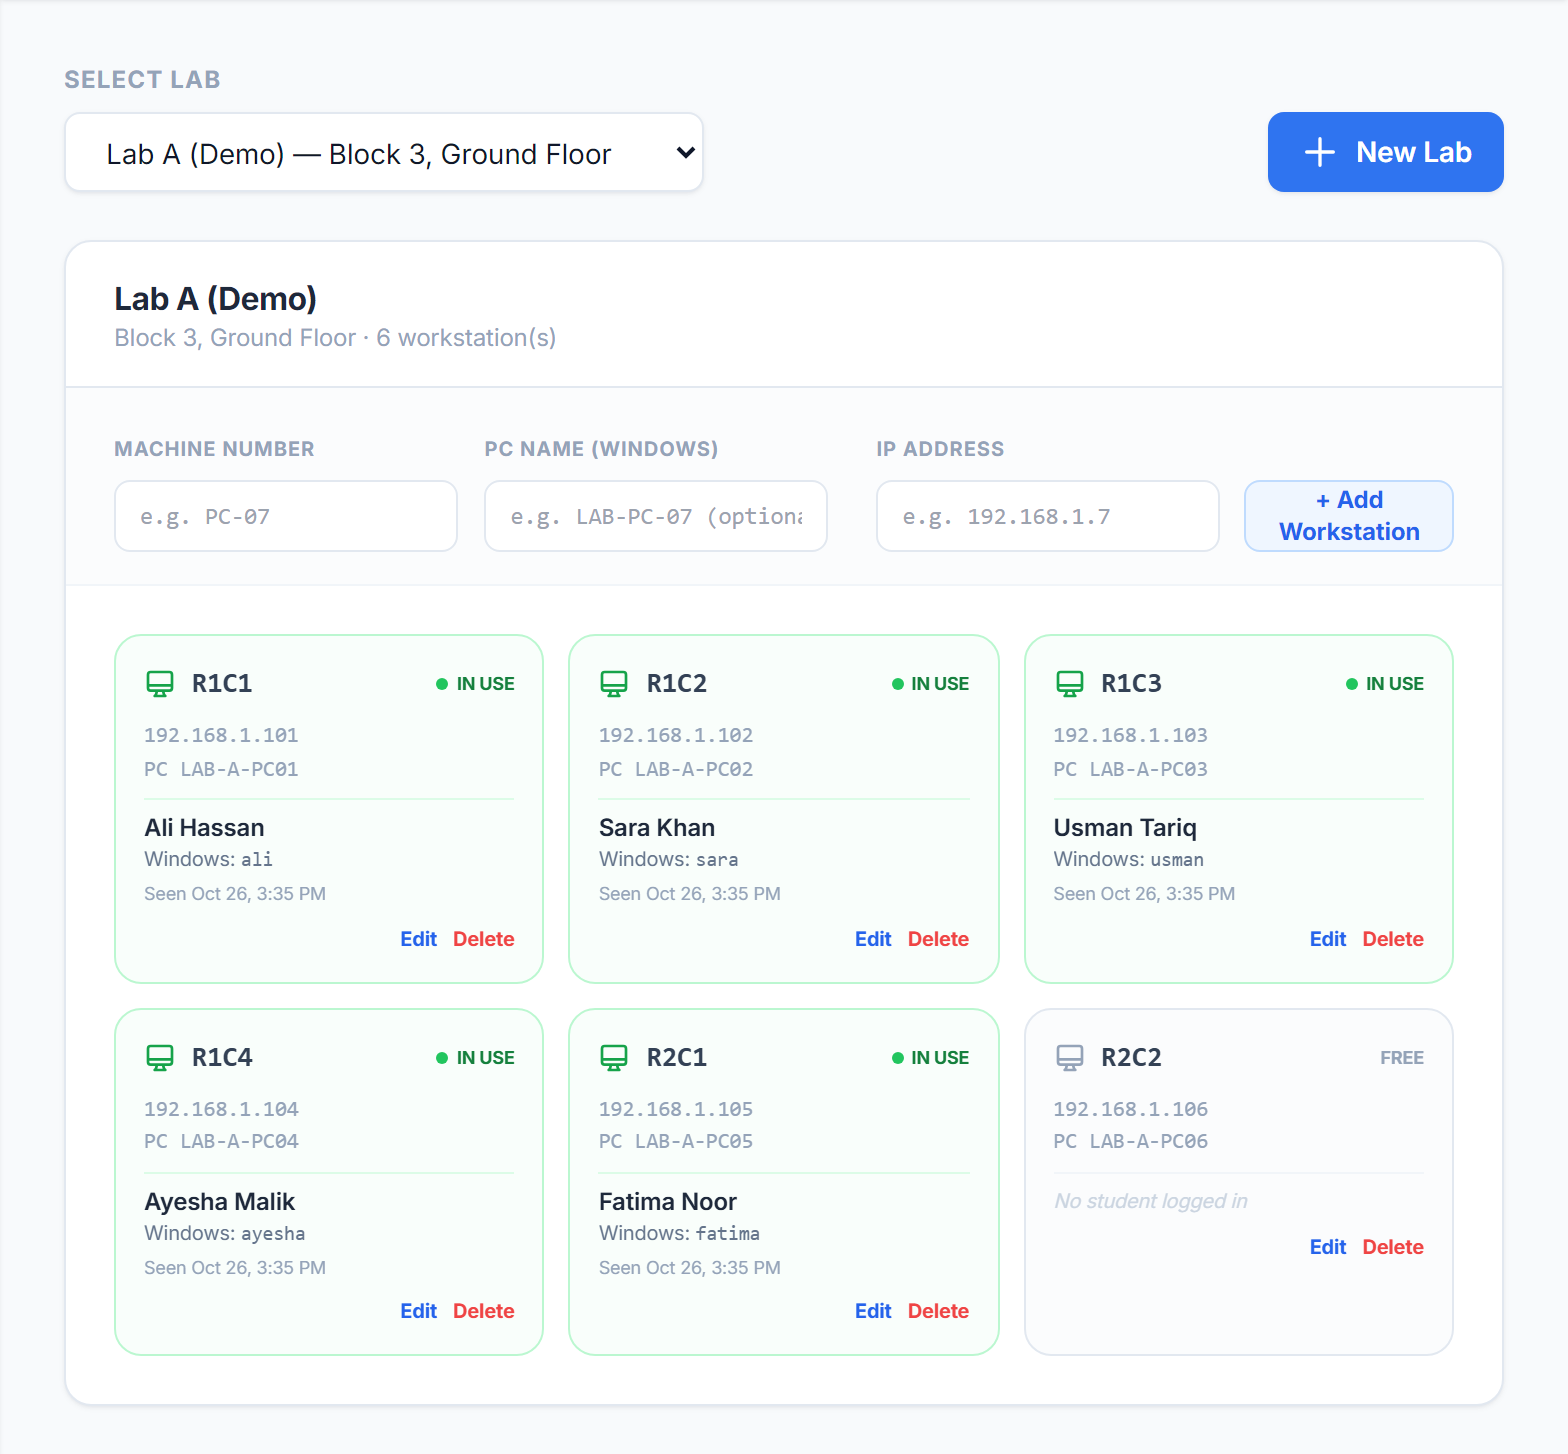
\includegraphics[width=\linewidth,height=418pt,keepaspectratio]{Figures/ui_labs_workstations.png}
\caption{Labs and Workstations}
\label{fig:ui_labs_workstations}
\end{figure}
\SoftBarrierN

The device-binding page (Figure~\ref{fig:ui_device_bindings}) lists each student's binding status, bound PC and last-seen time (FR1). \emph{Reset Binding} (\texttt{DELETE /api/users/\{id\}/device-binding}) removes the binding and revokes all the student's tokens, so the next login binds a new PC; \emph{Force Logout} only revokes the tokens. In the figure the five students who have signed in are \emph{Bound} to LAB-A-PC01 to LAB-A-PC05, while Hamza Iqbal is \emph{Unbound}, so his row has no PC and no actions. A search box and a \emph{Show unbound only} switch help the administrator find a student, and the note at the top says that an administrator can reset a binding after a genuine hardware change or a login problem.

\begin{figure}[tbp]
\centering
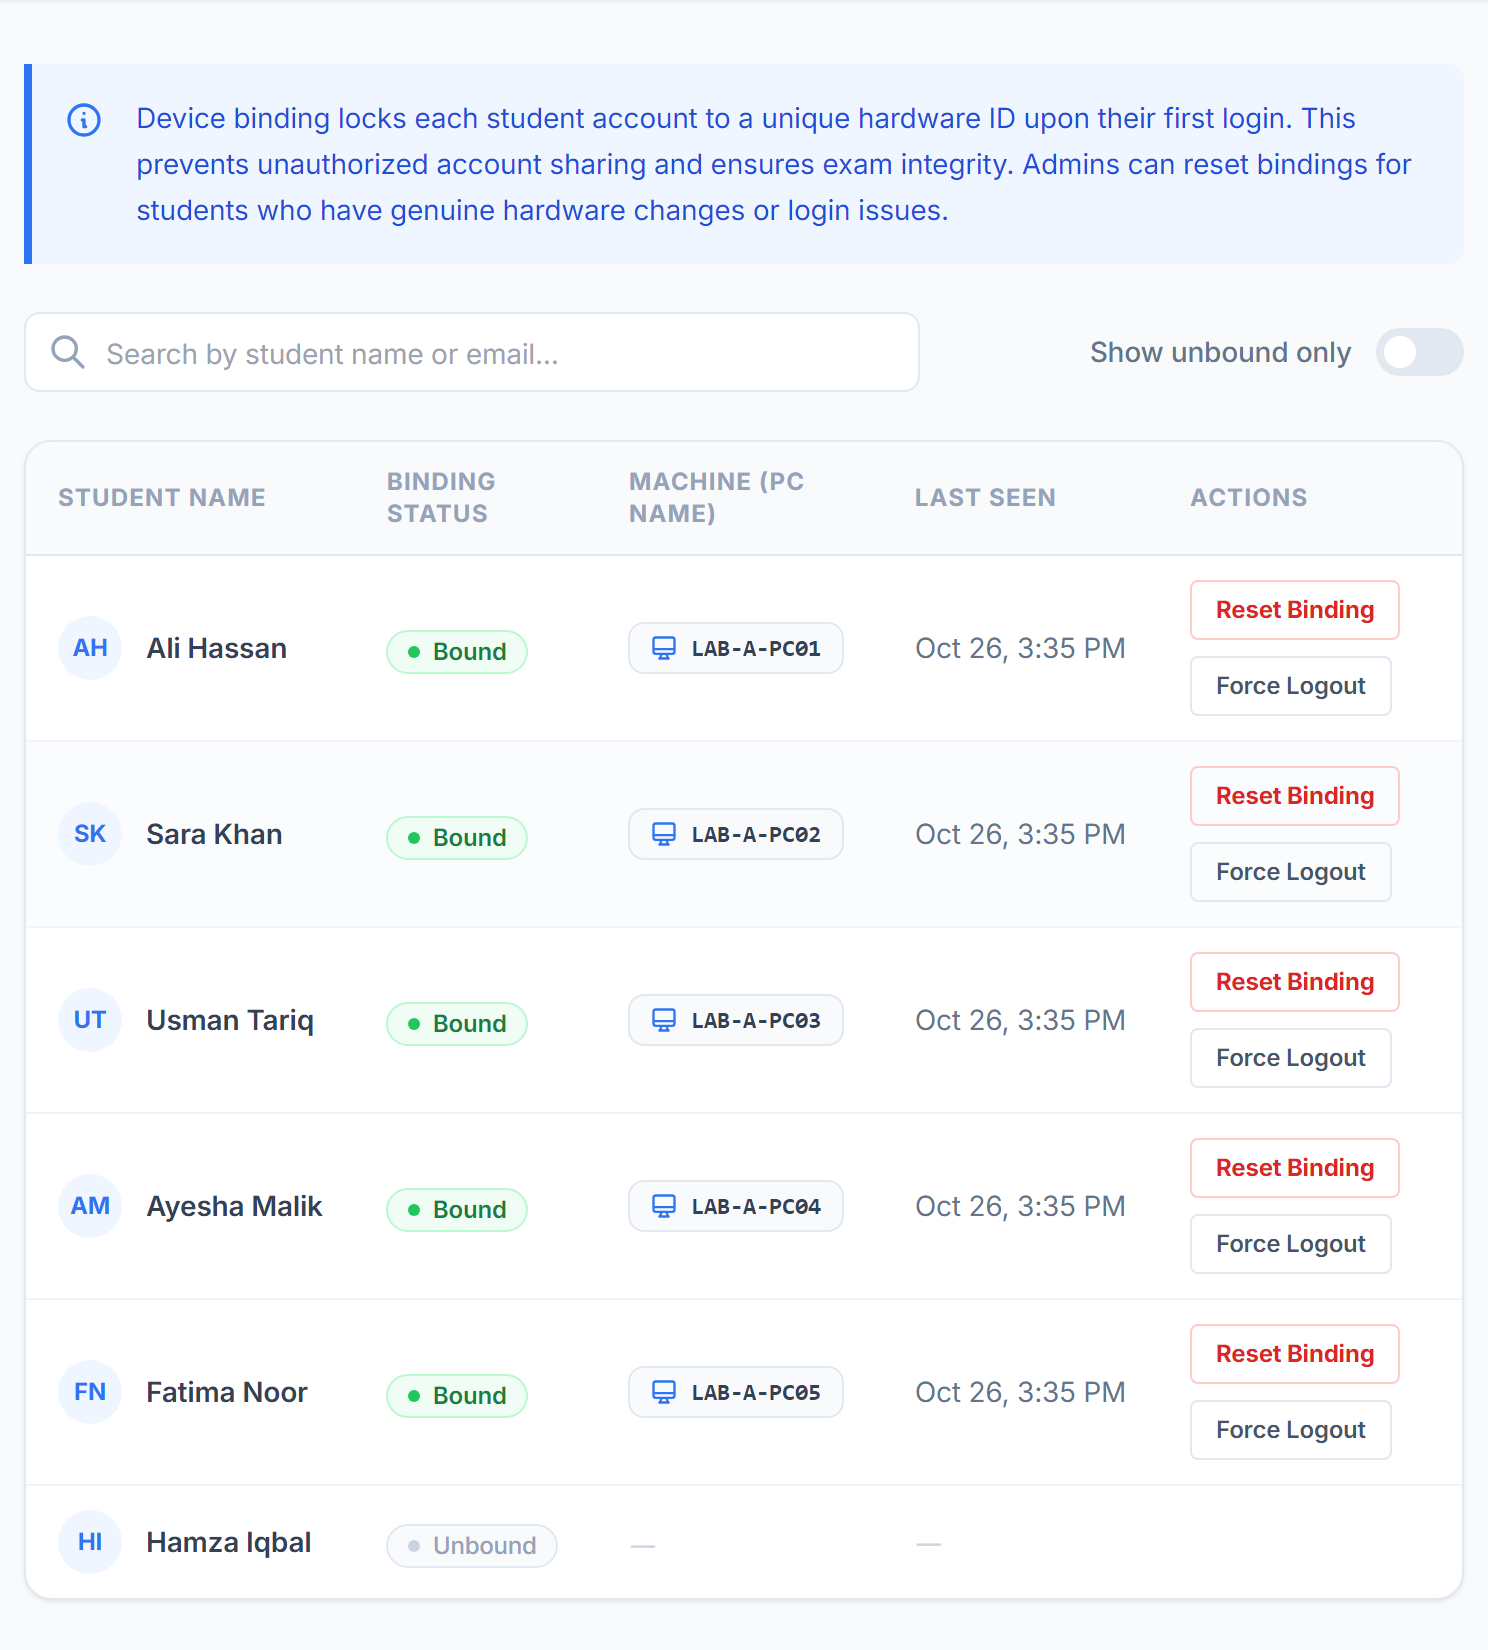
\includegraphics[width=\linewidth,height=500pt,keepaspectratio]{Figures/ui_device_bindings.png}
\caption{Device Bindings (Email, Windows User and Registered Columns Omitted)}
\label{fig:ui_device_bindings}
\end{figure}
\SoftBarrierN

The read-only audit page (Figure~\ref{fig:ui_audit_logs}) lists \texttt{AuditLogs} rows (time, actor, event, entity, JSON details) for security-relevant and staff actions, such as logins, grade overrides, completed AI grading and submissions (FR12). The newest rows come first, and the actor is a user with an email or \emph{System} for background jobs. The visible rows follow the end of the demo exam, from the warning sent to Usman (\texttt{PROCTOR\_WARNING\_SENT}, 3:35:43~PM) through three submissions (\texttt{SESSION\_SUBMITTED}) and the background grading (\texttt{AI\_GRADING\_COMPLETED}) to a grade override by Dr. Ahmed and a new login by Ali Hassan. The green badge \emph{Chain verified (91 entries)} at the top shows that the hash chain over these rows verifies, and \emph{Re-verify} runs the check again.

\begin{figure}[tbp]
\centering
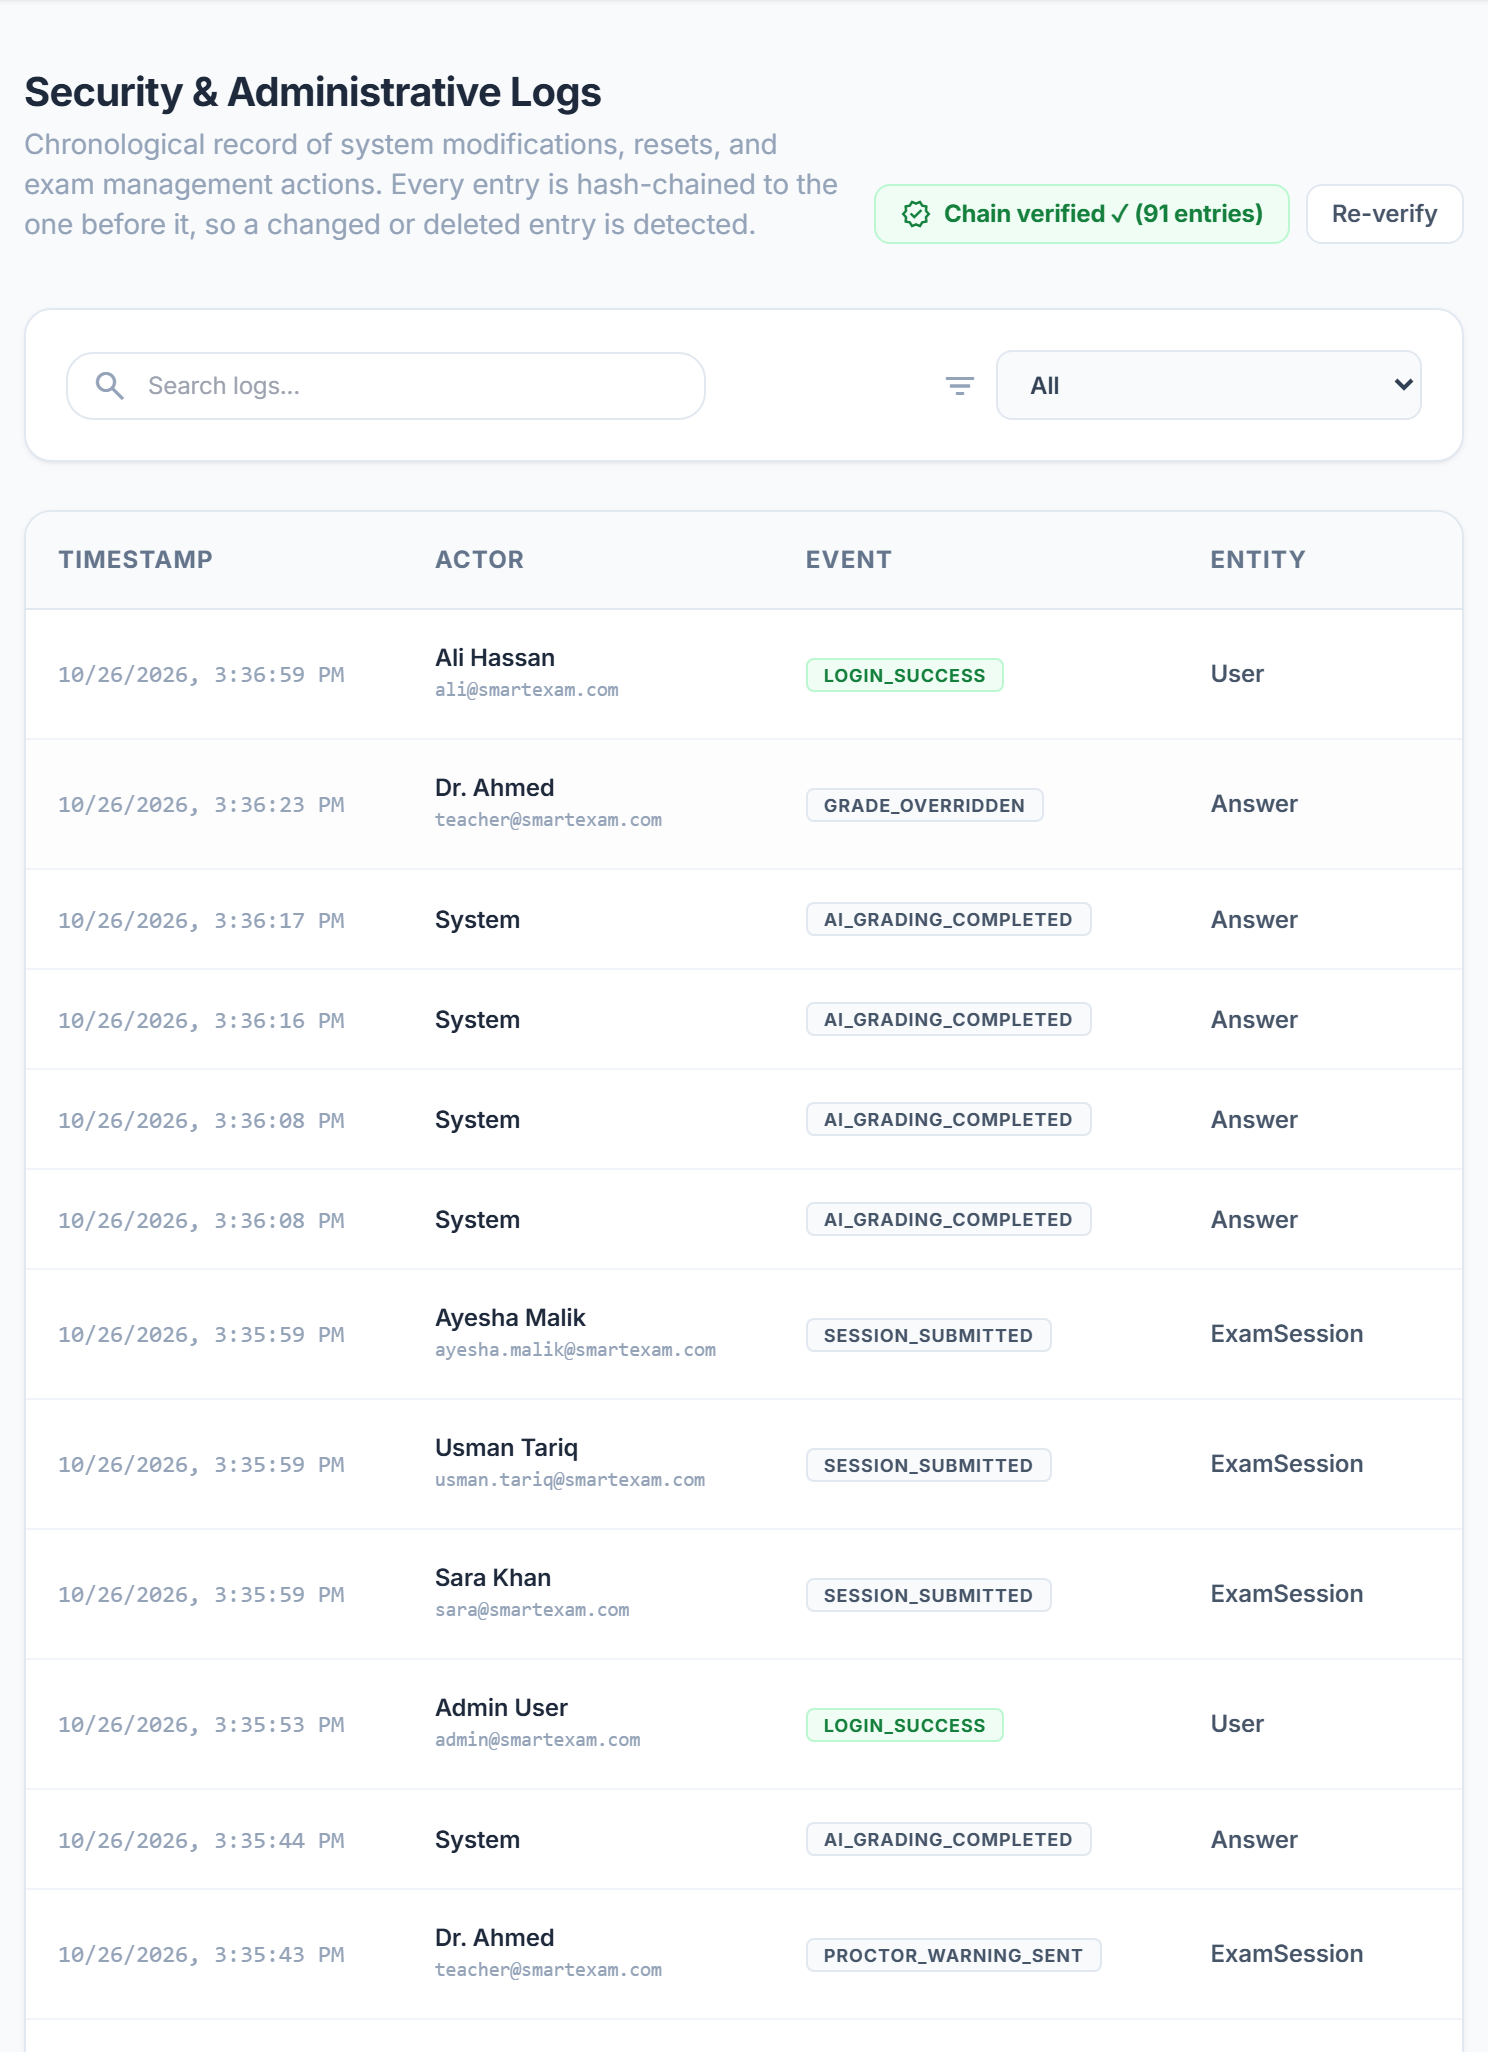
\includegraphics[width=\linewidth,height=622pt,keepaspectratio]{Figures/ui_audit_logs.png}
\caption{Audit Log Page (Details Column Omitted)}
\label{fig:ui_audit_logs}
\end{figure}
\SoftBarrierN

In the student portal (Figures~\ref{fig:ui_student_performance} to~\ref{fig:ui_student_performance_b}) a student sees exams taken, average and best score, integrity flags, a score trend, the score of each exam and an exam timeline; practice exams do not count towards results (they are auto-marked but never plagiarism-checked and are hidden from the student's results). The summary cards (Figure~\ref{fig:ui_student_performance}) show four exams taken, an average of 85.9\,\%, a best score of 93.3\,\% and no flags; the flag count adds up the violations recorded in the student's sessions. The average matches the mean of the four scores in the timeline (80, 83.3, 93.3 and 87.1\,\%).

\begin{figure}[tbp]
\centering
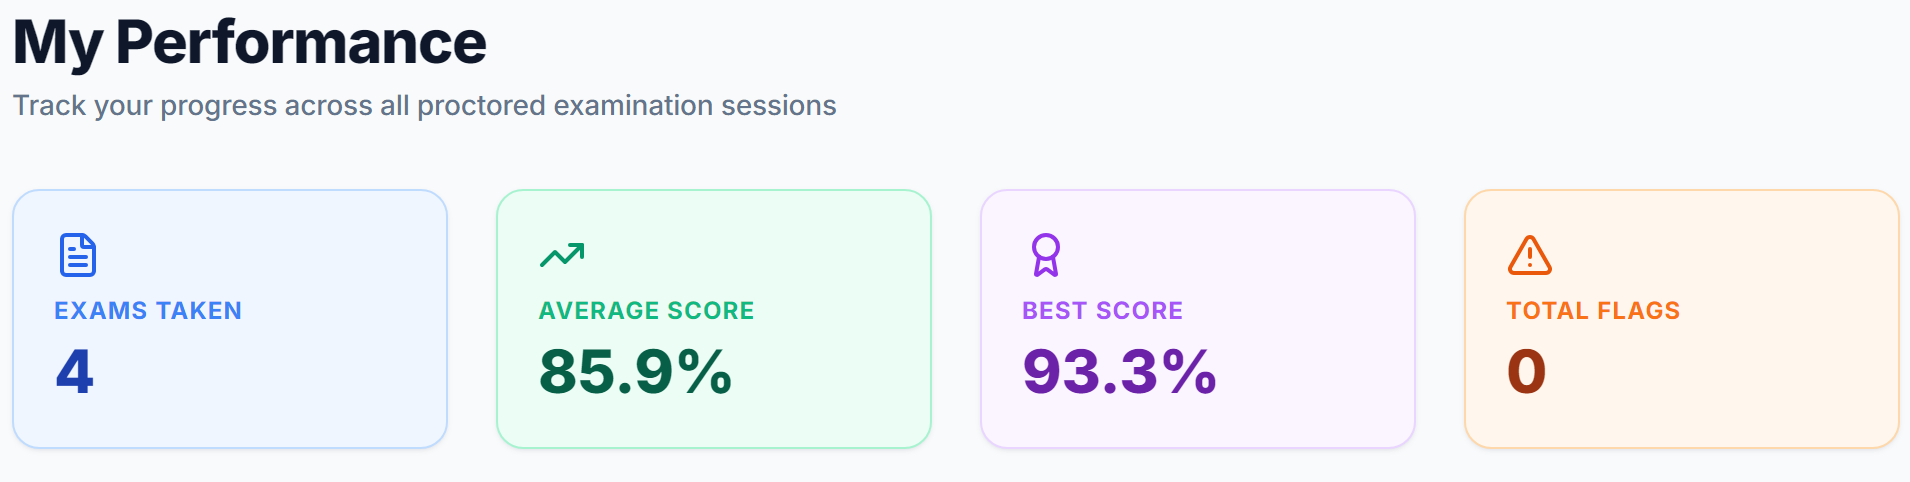
\includegraphics[width=\linewidth]{Figures/ui_student_performance_a_p1.png}
\caption{Student Performance Page (a): Summary Cards}
\label{fig:ui_student_performance}
\end{figure}
\SoftBarrierN

The \emph{Score Over Time} chart (Figure~\ref{fig:ui_student_performance_trend}) draws the same scores in date order, from Lab Exam~1 to the Mid-Term Lab Exam, above a dashed pass-mark line at 50\,\%. The \emph{Improving trend} badge appears because the latest score is higher than the first one. Figure~\ref{fig:ui_student_performance_b} shows the four exams again as bars, with the score rounded to a whole percent, and as a timeline, newest first, with the date and exact score of each exam.

\begin{figure}[tbp]
\centering
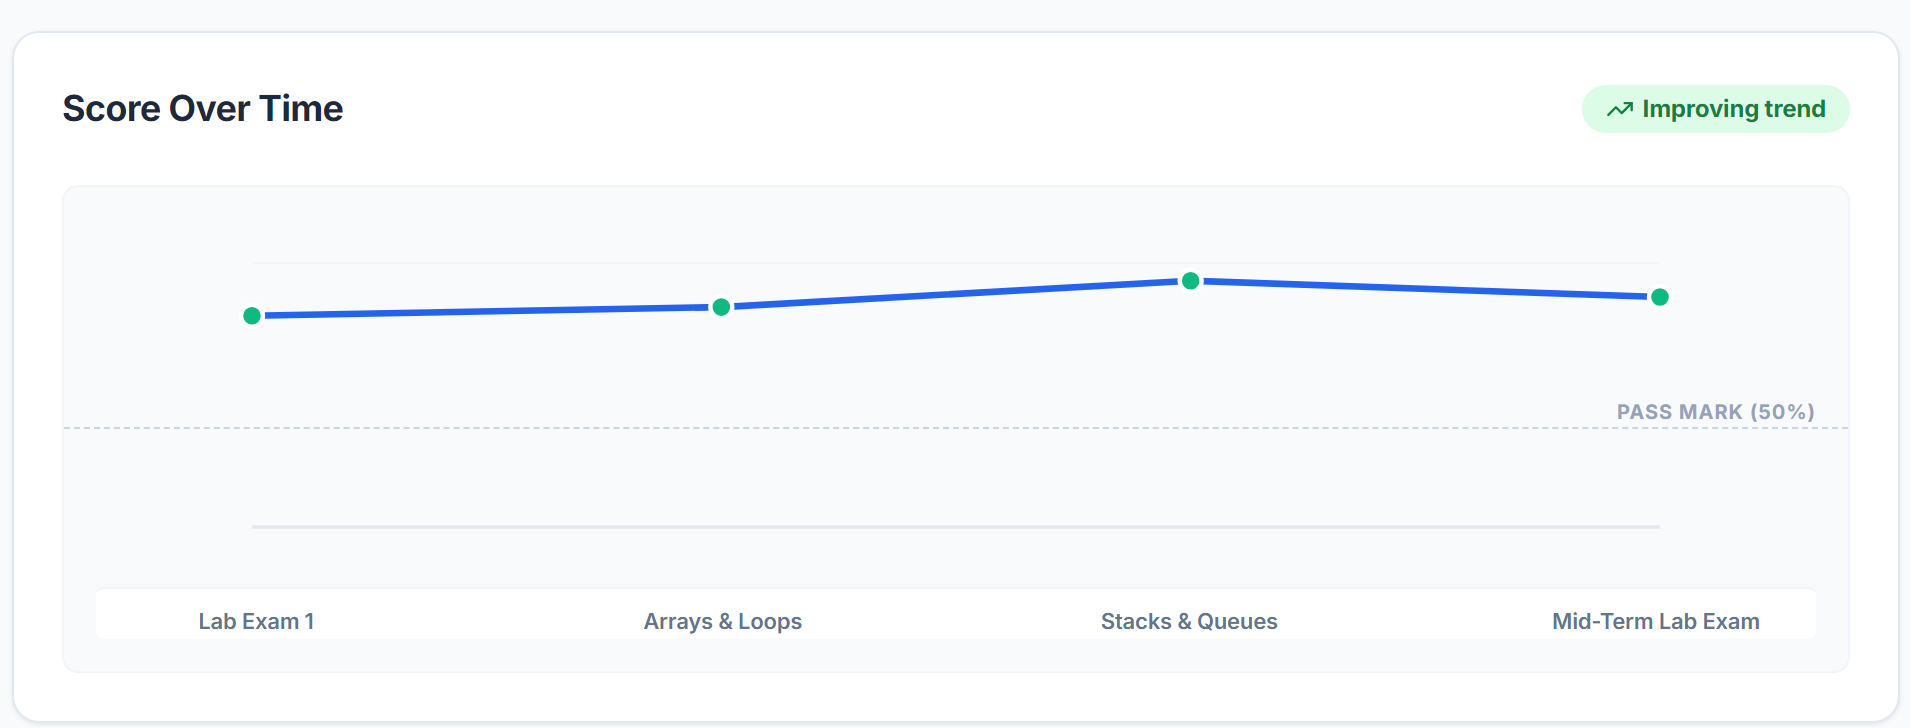
\includegraphics[width=\linewidth]{Figures/ui_student_performance_a_p2.png}
\caption{Student Performance Page (b): Score Trend}
\label{fig:ui_student_performance_trend}
\end{figure}
\SoftBarrierN

\begin{figure}[tbp]
\centering
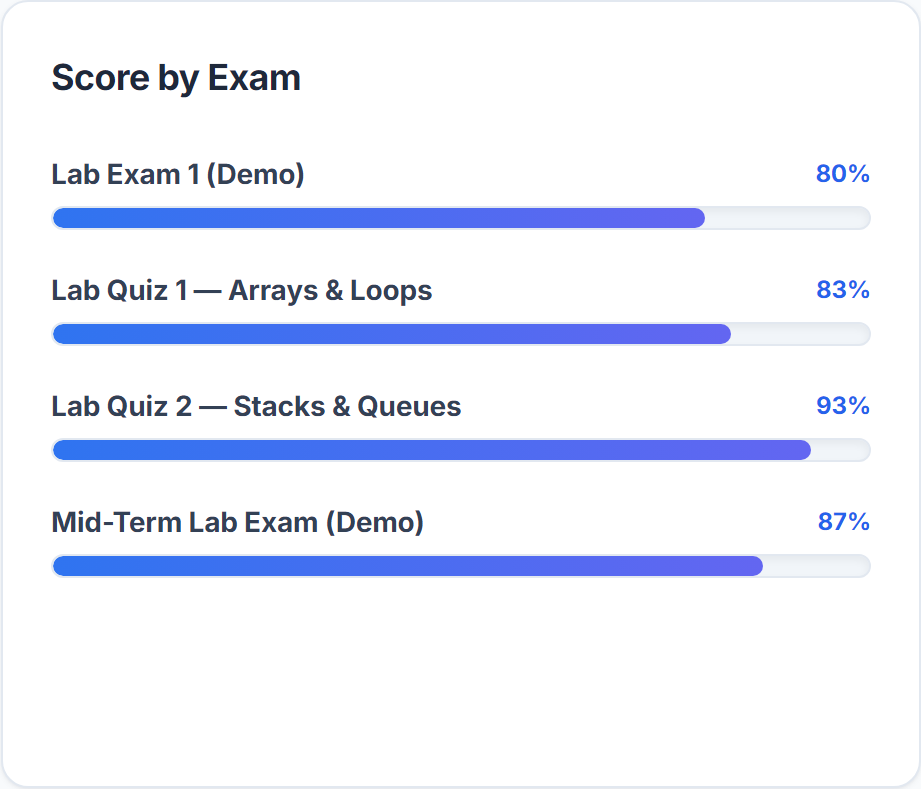
\includegraphics[width=0.7\linewidth]{Figures/ui_student_performance_scores.png}\\[4pt]
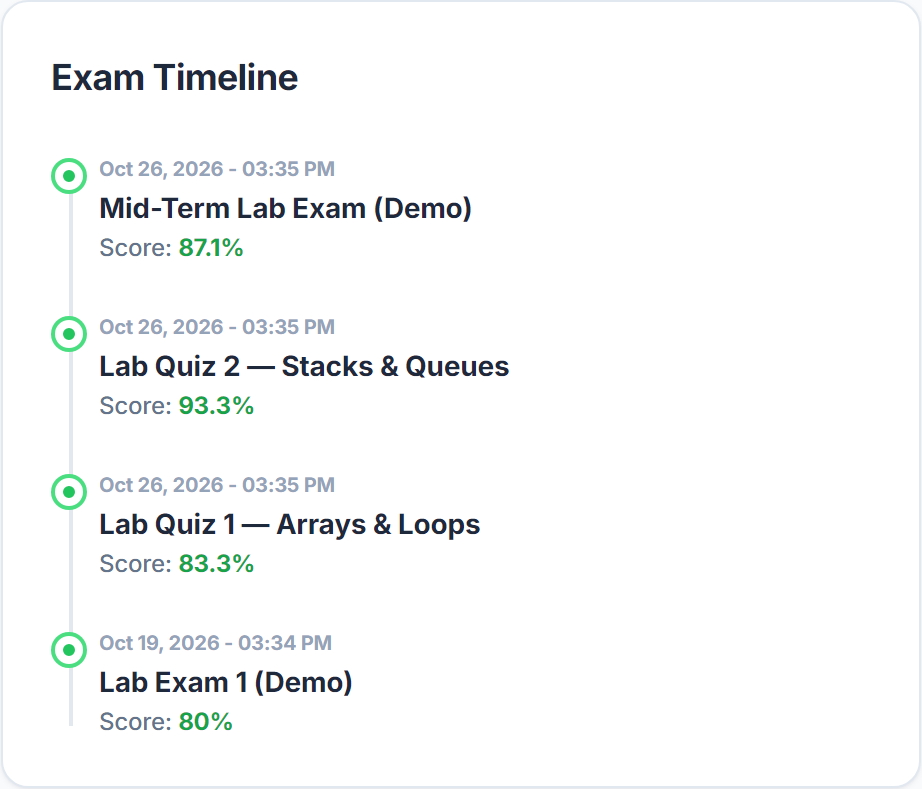
\includegraphics[width=0.7\linewidth]{Figures/ui_student_performance_timeline.png}
\caption{Student Performance Page (c): Score by Exam and Exam Timeline Cards}
\label{fig:ui_student_performance_b}
\end{figure}
\SoftBarrierN

\clearpage
\renewcommand{\topfraction}{0.7}\renewcommand{\bottomfraction}{0.3}
\renewcommand{\textfraction}{0.2}\renewcommand{\floatpagefraction}{0.5}
\section{Physical Database Tables}
\label{sec:physical_tables}
% Database tables, one per entity of the ERD (Figure~\ref{fig:erd_diagram}).
The database tables below follow the entity relationship diagram in Figure~\ref{fig:erd_diagram}, with one table for each of its 14 entities. Each table lists its fields, the data type of each field, its key or constraint, and a short description. PK marks a primary key, FK marks a foreign key, and Unique marks a field that may not repeat in the table.

\subsection{Roles Table}
The Roles table stores the names of the user roles in the system. Each user belongs to one role, and one role can be given to many users.

{\small
\begin{longtable}{>{\raggedright\arraybackslash}p{3.4cm}>{\raggedright\arraybackslash}p{2.9cm}>{\raggedright\arraybackslash}p{2.3cm}>{\raggedright\arraybackslash}p{5.6cm}}
\caption{Roles Table}\label{tab:db_roles}\\
\hline\hline
\textbf{Field Name} & \textbf{Data Type} & \textbf{Key / Constraint} & \textbf{Description} \\ \hline
\endfirsthead
\multicolumn{4}{c}{\tablename~\thetable{} -- continued from previous page}\\
\hline\hline
\textbf{Field Name} & \textbf{Data Type} & \textbf{Key / Constraint} & \textbf{Description} \\ \hline
\endhead
\hline \multicolumn{4}{r}{Continued on next page}\\
\endfoot
\hline\hline
\endlastfoot
Id & INT & PK & Unique number of the role \\
RoleName & VARCHAR(50) & -- & Name of the role \\
\end{longtable}
}

\subsection{Users Table}
The Users table stores the accounts of everyone who uses the system. Each user is linked to one role through RoleId. A user can have one device binding and can be linked to many exams, audit log entries, exam sessions and seating map entries.

{\small
\begin{longtable}{>{\raggedright\arraybackslash}p{3.4cm}>{\raggedright\arraybackslash}p{2.9cm}>{\raggedright\arraybackslash}p{2.3cm}>{\raggedright\arraybackslash}p{5.6cm}}
\caption{Users Table}\label{tab:db_users}\\
\hline\hline
\textbf{Field Name} & \textbf{Data Type} & \textbf{Key / Constraint} & \textbf{Description} \\ \hline
\endfirsthead
\multicolumn{4}{c}{\tablename~\thetable{} -- continued from previous page}\\
\hline\hline
\textbf{Field Name} & \textbf{Data Type} & \textbf{Key / Constraint} & \textbf{Description} \\ \hline
\endhead
\hline \multicolumn{4}{r}{Continued on next page}\\
\endfoot
\hline\hline
\endlastfoot
Id & INT & PK & Unique number of the user \\
Email & VARCHAR(255) & -- & Email address of the user \\
PasswordHash & VARCHAR(255) & -- & Hash of the user's password \\
FullName & VARCHAR(255) & -- & Full name of the user \\
RoleId & INT & FK & Role of the user (Roles) \\
CreatedAt & TIMESTAMP & -- & Time the account was created \\
\end{longtable}
}

\subsection{DeviceBindings Table}
The DeviceBindings table stores the device that is bound to a user. UserId is unique, so each user has at most one binding and each binding belongs to one user.

{\small
\begin{longtable}{>{\raggedright\arraybackslash}p{3.4cm}>{\raggedright\arraybackslash}p{2.9cm}>{\raggedright\arraybackslash}p{2.3cm}>{\raggedright\arraybackslash}p{5.6cm}}
\caption{DeviceBindings Table}\label{tab:db_devicebindings}\\
\hline\hline
\textbf{Field Name} & \textbf{Data Type} & \textbf{Key / Constraint} & \textbf{Description} \\ \hline
\endfirsthead
\multicolumn{4}{c}{\tablename~\thetable{} -- continued from previous page}\\
\hline\hline
\textbf{Field Name} & \textbf{Data Type} & \textbf{Key / Constraint} & \textbf{Description} \\ \hline
\endhead
\hline \multicolumn{4}{r}{Continued on next page}\\
\endfoot
\hline\hline
\endlastfoot
Id & INT & PK & Unique number of the binding \\
UserId & INT & FK, Unique & User the device is bound to (Users) \\
HWID & VARCHAR(255) & -- & Hardware ID of the device \\
DeviceDetails & TEXT & -- & Details of the device \\
BoundAt & TIMESTAMP & -- & Time the device was bound \\
\end{longtable}
}

\subsection{Exams Table}
The Exams table stores each exam and its schedule. CreatedBy links the exam to the user who created it. One exam can have many questions, allowed apps, exam sessions, seating map entries and plagiarism results.

{\small
\begin{longtable}{>{\raggedright\arraybackslash}p{3.4cm}>{\raggedright\arraybackslash}p{2.9cm}>{\raggedright\arraybackslash}p{2.3cm}>{\raggedright\arraybackslash}p{5.6cm}}
\caption{Exams Table}\label{tab:db_exams}\\
\hline\hline
\textbf{Field Name} & \textbf{Data Type} & \textbf{Key / Constraint} & \textbf{Description} \\ \hline
\endfirsthead
\multicolumn{4}{c}{\tablename~\thetable{} -- continued from previous page}\\
\hline\hline
\textbf{Field Name} & \textbf{Data Type} & \textbf{Key / Constraint} & \textbf{Description} \\ \hline
\endhead
\hline \multicolumn{4}{r}{Continued on next page}\\
\endfoot
\hline\hline
\endlastfoot
Id & INT & PK & Unique number of the exam \\
Title & VARCHAR(255) & -- & Title of the exam \\
Description & TEXT & -- & Description of the exam \\
Duration & INT & -- & Length of the exam \\
StartTime & TIMESTAMP & -- & Time the exam starts \\
EndTime & TIMESTAMP & -- & Time the exam ends \\
IsActive & BOOLEAN & -- & Whether the exam is active \\
CreatedBy & INT & FK & User who created the exam (Users) \\
\end{longtable}
}

\subsection{AuditLogs Table}
The AuditLogs table stores a record of actions taken in the system. Each entry is linked to the user who performed the action, and one user can have many entries.

{\small
\begin{longtable}{>{\raggedright\arraybackslash}p{3.4cm}>{\raggedright\arraybackslash}p{2.9cm}>{\raggedright\arraybackslash}p{2.3cm}>{\raggedright\arraybackslash}p{5.6cm}}
\caption{AuditLogs Table}\label{tab:db_auditlogs}\\
\hline\hline
\textbf{Field Name} & \textbf{Data Type} & \textbf{Key / Constraint} & \textbf{Description} \\ \hline
\endfirsthead
\multicolumn{4}{c}{\tablename~\thetable{} -- continued from previous page}\\
\hline\hline
\textbf{Field Name} & \textbf{Data Type} & \textbf{Key / Constraint} & \textbf{Description} \\ \hline
\endhead
\hline \multicolumn{4}{r}{Continued on next page}\\
\endfoot
\hline\hline
\endlastfoot
Id & INT & PK & Unique number of the log entry \\
UserId & INT & FK & User who performed the action (Users) \\
Action & VARCHAR(100) & -- & Name of the action \\
ActionDetails & TEXT & -- & Details of the action \\
Timestamp & TIMESTAMP & -- & Time the action took place \\
\end{longtable}
}

\subsection{ExamSessions Table}
The ExamSessions table stores one user's attempt at an exam. Each session is linked to one exam and one user. A session can have many monitoring events and many answers.

{\small
\begin{longtable}{>{\raggedright\arraybackslash}p{3.4cm}>{\raggedright\arraybackslash}p{2.9cm}>{\raggedright\arraybackslash}p{2.3cm}>{\raggedright\arraybackslash}p{5.6cm}}
\caption{ExamSessions Table}\label{tab:db_examsessions}\\
\hline\hline
\textbf{Field Name} & \textbf{Data Type} & \textbf{Key / Constraint} & \textbf{Description} \\ \hline
\endfirsthead
\multicolumn{4}{c}{\tablename~\thetable{} -- continued from previous page}\\
\hline\hline
\textbf{Field Name} & \textbf{Data Type} & \textbf{Key / Constraint} & \textbf{Description} \\ \hline
\endhead
\hline \multicolumn{4}{r}{Continued on next page}\\
\endfoot
\hline\hline
\endlastfoot
Id & INT & PK & Unique number of the session \\
ExamId & INT & FK & Exam being taken (Exams) \\
UserId & INT & FK & User taking the exam (Users) \\
StartTime & TIMESTAMP & -- & Time the session started \\
EndTime & TIMESTAMP & -- & Time the session ended \\
RemainingTime & INT & -- & Time left in the session \\
Status & VARCHAR(50) & -- & Current status of the session \\
\end{longtable}
}

\subsection{AllowedApps Table}
The AllowedApps table stores the applications that may be used during an exam. Each entry belongs to one exam, and one exam can have many allowed apps.

{\small
\begin{longtable}{>{\raggedright\arraybackslash}p{3.4cm}>{\raggedright\arraybackslash}p{2.9cm}>{\raggedright\arraybackslash}p{2.3cm}>{\raggedright\arraybackslash}p{5.6cm}}
\caption{AllowedApps Table}\label{tab:db_allowedapps}\\
\hline\hline
\textbf{Field Name} & \textbf{Data Type} & \textbf{Key / Constraint} & \textbf{Description} \\ \hline
\endfirsthead
\multicolumn{4}{c}{\tablename~\thetable{} -- continued from previous page}\\
\hline\hline
\textbf{Field Name} & \textbf{Data Type} & \textbf{Key / Constraint} & \textbf{Description} \\ \hline
\endhead
\hline \multicolumn{4}{r}{Continued on next page}\\
\endfoot
\hline\hline
\endlastfoot
Id & INT & PK & Unique number of the entry \\
ExamId & INT & FK & Exam the app is allowed in (Exams) \\
AppName & VARCHAR(100) & -- & Name of the allowed application \\
\end{longtable}
}

\subsection{Questions Table}
The Questions table stores the questions of each exam. Each question belongs to one exam. One question can have many answers and many test cases.

{\small
\begin{longtable}{>{\raggedright\arraybackslash}p{3.4cm}>{\raggedright\arraybackslash}p{2.9cm}>{\raggedright\arraybackslash}p{2.3cm}>{\raggedright\arraybackslash}p{5.6cm}}
\caption{Questions Table}\label{tab:db_questions}\\
\hline\hline
\textbf{Field Name} & \textbf{Data Type} & \textbf{Key / Constraint} & \textbf{Description} \\ \hline
\endfirsthead
\multicolumn{4}{c}{\tablename~\thetable{} -- continued from previous page}\\
\hline\hline
\textbf{Field Name} & \textbf{Data Type} & \textbf{Key / Constraint} & \textbf{Description} \\ \hline
\endhead
\hline \multicolumn{4}{r}{Continued on next page}\\
\endfoot
\hline\hline
\endlastfoot
Id & INT & PK & Unique number of the question \\
ExamId & INT & FK & Exam the question belongs to (Exams) \\
QuestionText & TEXT & -- & Text of the question \\
QuestionType & VARCHAR(50) & -- & Type of the question \\
MaxMarks & INT & -- & Highest marks for the question \\
\end{longtable}
}

\subsection{SeatingMaps Table}
The SeatingMaps table stores where each user sits for an exam. Each entry is linked to one exam and one user, and gives the lab, IP range and seat number.

{\small
\begin{longtable}{>{\raggedright\arraybackslash}p{3.4cm}>{\raggedright\arraybackslash}p{2.9cm}>{\raggedright\arraybackslash}p{2.3cm}>{\raggedright\arraybackslash}p{5.6cm}}
\caption{SeatingMaps Table}\label{tab:db_seatingmaps}\\
\hline\hline
\textbf{Field Name} & \textbf{Data Type} & \textbf{Key / Constraint} & \textbf{Description} \\ \hline
\endfirsthead
\multicolumn{4}{c}{\tablename~\thetable{} -- continued from previous page}\\
\hline\hline
\textbf{Field Name} & \textbf{Data Type} & \textbf{Key / Constraint} & \textbf{Description} \\ \hline
\endhead
\hline \multicolumn{4}{r}{Continued on next page}\\
\endfoot
\hline\hline
\endlastfoot
Id & INT & PK & Unique number of the entry \\
ExamId & INT & FK & Exam the seat is for (Exams) \\
UserId & INT & FK & User given the seat (Users) \\
LabName & VARCHAR(100) & -- & Name of the lab \\
IPRange & VARCHAR(100) & -- & IP address range of the lab \\
SeatNumber & VARCHAR(50) & -- & Seat number given to the user \\
\end{longtable}
}

\subsection{MonitoringEvents Table}
The MonitoringEvents table stores the events recorded while a user takes an exam. Each event belongs to one exam session, and one session can have many events.

{\small
\begin{longtable}{>{\raggedright\arraybackslash}p{3.4cm}>{\raggedright\arraybackslash}p{2.9cm}>{\raggedright\arraybackslash}p{2.3cm}>{\raggedright\arraybackslash}p{5.6cm}}
\caption{MonitoringEvents Table}\label{tab:db_monitoringevents}\\
\hline\hline
\textbf{Field Name} & \textbf{Data Type} & \textbf{Key / Constraint} & \textbf{Description} \\ \hline
\endfirsthead
\multicolumn{4}{c}{\tablename~\thetable{} -- continued from previous page}\\
\hline\hline
\textbf{Field Name} & \textbf{Data Type} & \textbf{Key / Constraint} & \textbf{Description} \\ \hline
\endhead
\hline \multicolumn{4}{r}{Continued on next page}\\
\endfoot
\hline\hline
\endlastfoot
Id & INT & PK & Unique number of the event \\
SessionId & INT & FK & Session the event belongs to (ExamSessions) \\
EventType & VARCHAR(100) & -- & Type of the event \\
EventDetails & TEXT & -- & Details of the event \\
ScreenshotUrl & VARCHAR(255) & -- & Link to the screenshot of the event \\
Timestamp & TIMESTAMP & -- & Time the event took place \\
\end{longtable}
}

\subsection{Answers Table}
The Answers table stores the answers given in an exam. Each answer is linked to one exam session and one question. Each answer has one AI grading result and can appear in many plagiarism results.

{\small
\begin{longtable}{>{\raggedright\arraybackslash}p{3.4cm}>{\raggedright\arraybackslash}p{2.9cm}>{\raggedright\arraybackslash}p{2.3cm}>{\raggedright\arraybackslash}p{5.6cm}}
\caption{Answers Table}\label{tab:db_answers}\\
\hline\hline
\textbf{Field Name} & \textbf{Data Type} & \textbf{Key / Constraint} & \textbf{Description} \\ \hline
\endfirsthead
\multicolumn{4}{c}{\tablename~\thetable{} -- continued from previous page}\\
\hline\hline
\textbf{Field Name} & \textbf{Data Type} & \textbf{Key / Constraint} & \textbf{Description} \\ \hline
\endhead
\hline \multicolumn{4}{r}{Continued on next page}\\
\endfoot
\hline\hline
\endlastfoot
Id & INT & PK & Unique number of the answer \\
SessionId & INT & FK & Session the answer was given in (ExamSessions) \\
QuestionId & INT & FK & Question being answered (Questions) \\
AnswerText & TEXT & -- & Text of the answer \\
LastSavedAt & TIMESTAMP & -- & Time the answer was last saved \\
\end{longtable}
}

\subsection{TestCases Table}
The TestCases table stores the test cases of a question. Each test case belongs to one question and gives an input with its expected output.

{\small
\begin{longtable}{>{\raggedright\arraybackslash}p{3.4cm}>{\raggedright\arraybackslash}p{2.9cm}>{\raggedright\arraybackslash}p{2.3cm}>{\raggedright\arraybackslash}p{5.6cm}}
\caption{TestCases Table}\label{tab:db_testcases}\\
\hline\hline
\textbf{Field Name} & \textbf{Data Type} & \textbf{Key / Constraint} & \textbf{Description} \\ \hline
\endfirsthead
\multicolumn{4}{c}{\tablename~\thetable{} -- continued from previous page}\\
\hline\hline
\textbf{Field Name} & \textbf{Data Type} & \textbf{Key / Constraint} & \textbf{Description} \\ \hline
\endhead
\hline \multicolumn{4}{r}{Continued on next page}\\
\endfoot
\hline\hline
\endlastfoot
Id & INT & PK & Unique number of the test case \\
QuestionId & INT & FK & Question the test case belongs to (Questions) \\
Input & TEXT & -- & Input given to the program \\
ExpectedOutput & TEXT & -- & Output the program should give \\
IsHidden & BOOLEAN & -- & Whether the test case is hidden \\
\end{longtable}
}

\subsection{AiGradingResults Table}
The AiGradingResults table stores the AI grading result of an answer. AnswerId is unique, so each answer has exactly one grading result.

{\small
\begin{longtable}{>{\raggedright\arraybackslash}p{3.4cm}>{\raggedright\arraybackslash}p{2.9cm}>{\raggedright\arraybackslash}p{2.3cm}>{\raggedright\arraybackslash}p{5.6cm}}
\caption{AiGradingResults Table}\label{tab:db_aigradingresults}\\
\hline\hline
\textbf{Field Name} & \textbf{Data Type} & \textbf{Key / Constraint} & \textbf{Description} \\ \hline
\endfirsthead
\multicolumn{4}{c}{\tablename~\thetable{} -- continued from previous page}\\
\hline\hline
\textbf{Field Name} & \textbf{Data Type} & \textbf{Key / Constraint} & \textbf{Description} \\ \hline
\endhead
\hline \multicolumn{4}{r}{Continued on next page}\\
\endfoot
\hline\hline
\endlastfoot
Id & INT & PK & Unique number of the result \\
AnswerId & INT & FK, Unique & Answer that was graded (Answers) \\
AutoGrade & INT & -- & Grade given automatically \\
ExecutionTime & FLOAT & -- & Time taken to run the answer \\
SemanticSimilarity\-Score & FLOAT & -- & Semantic similarity score of the answer \\
AiFeedback & TEXT & -- & Feedback written by the AI \\
\end{longtable}
}

\subsection{PlagiarismResults Table}
The PlagiarismResults table stores the result of comparing two answers for plagiarism. Each result is linked to one exam and to the two answers that were compared, AnswerId1 and AnswerId2.

{\small
\begin{longtable}{>{\raggedright\arraybackslash}p{3.4cm}>{\raggedright\arraybackslash}p{2.9cm}>{\raggedright\arraybackslash}p{2.3cm}>{\raggedright\arraybackslash}p{5.6cm}}
\caption{PlagiarismResults Table}\label{tab:db_plagiarismresults}\\
\hline\hline
\textbf{Field Name} & \textbf{Data Type} & \textbf{Key / Constraint} & \textbf{Description} \\ \hline
\endfirsthead
\multicolumn{4}{c}{\tablename~\thetable{} -- continued from previous page}\\
\hline\hline
\textbf{Field Name} & \textbf{Data Type} & \textbf{Key / Constraint} & \textbf{Description} \\ \hline
\endhead
\hline \multicolumn{4}{r}{Continued on next page}\\
\endfoot
\hline\hline
\endlastfoot
Id & INT & PK & Unique number of the result \\
ExamId & INT & FK & Exam the answers belong to (Exams) \\
AnswerId1 & INT & FK & First answer compared (Answers) \\
AnswerId2 & INT & FK & Second answer compared (Answers) \\
SimilarityScore & FLOAT & -- & How similar the two answers are \\
FlaggedStatus & VARCHAR(50) & -- & Flag status of the pair \\
\end{longtable}
}

\chapter{TEST PLAN}
\label{chap:testing}

% Chapter 7 tables follow the department sample (Sample Test Case Tables): no vertical rules,
% a double rule above the header, a single rule under it, no rules between rows and a double rule at the end.
This chapter describes how SmartExam was tested: the objective, the test levels, the test management process and the test cases with their results. Every result reported here comes from one final automated regression run on 26 October 2026 (code commit \texttt{d8345f8}). Checks that need a real lab PC and were not executed in that run are not marked as passed.

\section{Objective of the Testing Phase}
\label{sec:test_objective}

Testing checks that each functional requirement FR1--FR12 (Table~\ref{tab:functionalrequirements}) works as specified and that the quality levels NFR1--NFR10 in Sections~\ref{sec:qualityattributes} and~\ref{sec:othernfr} are met \cite{iso25010, sommerville}. For an exam system three properties matter most: a student cannot sit an exam from the wrong PC or outside the allowed time, answers are not lost when the network or the client fails, and staff see only the exams and students they are responsible for. Testing is also used to find defects early; they are listed in the bugs report (Table~\ref{tab:bugs}).

\section{Levels of Tests for Testing Software}
\label{sec:test_levels}

\subsection{Unit Testing}
\begin{sloppypar}
Unit tests check one class at a time without a database, network or Windows API. In \texttt{Backend\_\allowbreak{}API.\allowbreak{}Tests} (xUnit 2.9) they cover pure services such as \texttt{PasswordHelper}, \texttt{ViolationClassifier}, \texttt{TestCaseScorer}, \texttt{OutputComparer}, \texttt{TheoryGrader} and the plagiarism engine. In \texttt{Student\_\allowbreak{}Desktop\_\allowbreak{}App.\allowbreak{}Tests} (xUnit, \texttt{net9.0-\allowbreak{}windows}) they cover the policy classes of the WPF client: \texttt{ReadinessPolicy}, \texttt{LockdownPolicy}, \texttt{AutosaveScheduler}, the offline save queue, \texttt{DeviceFingerprint} and \texttt{TokenRefreshGate}. These classes take plain values (latency, monitor count, registry values, a fake clock), so the rules can be tested on any Windows PC. A few backend unit rows (M9-U-01 to M9-U-03, M11-U-08 to M11-U-10, M12-U-01 to M12-U-03 and M12-U-05) check their rule through the in-memory test host instead; the tables say so. Unit test cases have the prefix UT (Section~\ref{subsec:unit_tests}).
\end{sloppypar}

\subsection{Integration Testing}
\begin{sloppypar}
Integration tests check that the API, the database layer, authentication and the SignalR hub work together. Two tools are used:
\begin{itemize}[nosep]
  \item \textbf{xUnit acceptance tests.} \texttt{TestWebAppFactory} (based on \texttt{WebApplication\allowbreak{}Factory<Program>}) and \texttt{TestHost} start the real ASP.NET Core pipeline in memory, with routing, JWT validation, role policies, the rate limiter and the hub. The PostgreSQL \texttt{DbContext} is replaced by an EF Core InMemory database per factory, seeded by \texttt{TestSeeder}.
  \item \textbf{Playwright \texttt{api} project.} Black-box HTTP tests against a separately started backend that check status codes, error codes and response bodies.
\end{itemize}
Integration test cases have the prefix IT (Section~\ref{sec:it_cases}).
\end{sloppypar}

\subsection{System Testing}
\begin{sloppypar}
System tests run complete user flows across the web panel, the backend and the student client. The Playwright \texttt{chromium} project drives the React panel in headless Chromium. In the same test, a student desktop-client simulator (\texttt{tests/\allowbreak{}support/\allowbreak{}studentClient.ts}) sends the HTTP calls of the WPF client: \texttt{student-\allowbreak{}login} with a hardware fingerprint, start, save-answer, heartbeat, violation events, captures and submit. A test can therefore check, for example, that a focus-loss event sent by a student appears on the teacher's Live Monitor. The WPF windows themselves are not driven by a UI automation tool; those checks are on the manual lab checklist. System test cases have the prefix ST (Section~\ref{subsec:system_tests}).
\end{sloppypar}

\section{Test Management Process}
\label{sec:test_management}

\subsection{Design the Test Strategy}
\begin{itemize}[nosep]
  \item \textbf{Requirement-based IDs.} Each module has test IDs of the form \texttt{M<module>-\allowbreak{}<layer>-\allowbreak{}<nn>} (security-hardening tests use \texttt{SEC-\allowbreak{}<layer>-\allowbreak{}<nn>}) in the test catalogue (\texttt{Docs/\allowbreak{}TEST\_CASES.md}), with layers U (unit), I (in-process integration), A (black-box API), E (browser end-to-end), D (desktop UI on a lab PC), M (manual lab check) and P (load). Every UT, IT and ST row gives its catalogue ID in the Test Data column.
  \item \textbf{Tests before or with the feature.} Tests for a feature not yet built are committed as pending (\texttt{Skip} in xUnit, \texttt{test.fixme} in Playwright) and are enabled in the change that adds the feature.
  \item \textbf{Isolation.} No test uses the Neon production database. The backend suites run on a fresh seeded in-memory database, and most tests create their own exams and users.
  \item \textbf{Defects.} Each defect (D-01 to D-49) is recorded with the test, review or implementation step that found it, and is then fixed; a test that found a defect stays in the suite as a regression test.
  \item \textbf{Entry and exit criteria.} Entry: the solution builds and the module's test cases are written. Exit: zero failed tests in all suites, no open defect, and every catalogue row marked as automated maps to at least one passing test.
\end{itemize}

\subsection{Test Objectives}
\begin{itemize}[nosep]
  \item \textbf{Functional verification:} each FR from FR1 to FR12 behaves as specified, including its error responses (\texttt{DEVICE\_\allowbreak{}MISMATCH}, \texttt{READINESS\_\allowbreak{}REQUIRED}, \texttt{EXAM\_\allowbreak{}NOT\_\allowbreak{}STARTED}, \texttt{SEAT\_\allowbreak{}MISMATCH}, \texttt{ALREADY\_\allowbreak{}SUBMITTED}, \texttt{DESKTOP\_\allowbreak{}CLIENT\_\allowbreak{}REQUIRED}). The parts of FR2--FR6, FR9 and FR10 that need a lab PC (desktop windows, keyboard and USB events, the webcam, crash relaunch, the wrong seat, the warning banner) are verified only at the decision-logic level and stay on the lab checklist (Table~\ref{tab:st_pending}).
  \item \textbf{Access control:} each role, exam owner and assigned invigilator sees only their own data; other users receive 401, 403 or 404.
  \item \textbf{Exam integrity:} the server enforces start time, deadline, seat and a single sitting, and returns a receipt hash on submission.
  \item \textbf{Resilience and regression:} answers and monitoring events survive network loss, client restart and crashes, and the full suite is rerun after every fix.
\end{itemize}

\subsection{Test Criteria}
Table~\ref{tab:test_criteria} lists measurable criteria for grading accuracy and for each non-functional requirement NFR1--NFR10, taken from the requirement and from the limits set in the code, with the tests that check them. Each row names one scenario, states its limit in numbers where the code sets one, and gives the catalogue IDs of the tests that check it. Where a criterion was not measured in the final run, such as the 40-client load target of NFR4 or HTTPS for NFR8, the row says so instead of claiming a pass.

{\small\setlength{\tabcolsep}{4pt}\setlength{\doublerulesep}{1pt}
\begin{longtable}{@{}P{2.8cm}P{8.9cm}P{3.6cm}@{}}
\caption{Test Criteria}\label{tab:test_criteria}\\ \hline\hline
\textbf{Test Scenario} & \textbf{Test Criteria Description} & \textbf{Verified by}\\ \hline
\endfirsthead
\multicolumn{3}{c}{\footnotesize\tablename~\thetable{} -- continued from previous page}\\ \hline\hline
\textbf{Test Scenario} & \textbf{Test Criteria Description} & \textbf{Verified by}\\ \hline
\endhead
\hline \multicolumn{3}{r}{\footnotesize Continued on next page}\\
\endfoot
\hline\hline
\endlastfoot
Grading accuracy (FR11.1--FR11.3) & MCQ answers get full or zero marks. A coding answer is scored by test-case weight (weights 1, 1, 2 with the two weight-1 cases passed gives 50\%). Plagiarism similarity is at least 90\% after renaming, at least 95\% after comment and layout changes, and below 30\% for different algorithms. & M11-U-01/02, M11-U-03, M11-U-08 to M11-U-10\\
NFR1 Security & Passwords are PBKDF2 hashes with 600,000 iterations, and an older hash is flagged for upgrade; access tokens live 1,800~s; a reused refresh token revokes its family; logins are rate-limited per IP (HTTP 429). Requests without a token get 401, a student calling a staff endpoint gets 403, and a login from a second PC gets 401 \texttt{DEVICE\_\allowbreak{}MISMATCH}. & SEC-U-01, SEC-U-02, M1-I-04, M1-I-03, SEC-I-04, SEC-A-02, SEC-A-03, M1-A-04\\
NFR2 Reliability & Offline events keep their order and survive a restart; failed answer saves are replayed in order; the local backup is encrypted (AES-256-GCM) and a modified file is rejected; the Task Manager policy is restored after a crash, and a running session can be resumed. & M5-U-01, M5-U-03, M6-U-06, M6-U-03, M6-U-04, M4-U-17, M6-U-09\\
NFR3 Usability & A failed login shows an error and stays on the login page; a student who opens an admin URL is redirected; every refused start returns an error code and message for the client to show. The desktop screens were not checked on a lab PC, and no formal user study was carried out. & M1-E-02, SEC-E-01, M2-I-02, M3-I-01, M9-I-06\\
NFR4 Performance & Readiness fails a PC whose best API round trip exceeds 2~s or whose clock differs from the server by more than 60~s. Autosave fires 10~s after an edit. A test-case run is stopped at its time limit (default 2~s) and the other cases still run. The load target for 40 clients (p95 below 2~s) is not yet measured. & M2-U-01, M2-U-02, M6-U-02, M11-U-05; M5-P-01 pending\\
NFR5 Maintainability & Every module M1--M12 has automated tests that run headless on one PC, and a full regression run takes under 20 minutes. & All suites (Table~\ref{tab:test_summary})\\
NFR6 Data Integrity & Saves after the deadline (plus the 2-minute grace) are refused and a late submission locks the session; an older revision gets 409 \texttt{STALE\_\allowbreak{}REVISION}; the client and the server compute the same SHA-256 receipt; a changed or deleted audit row breaks the hash chain. & M6-A-02, M6-I-06, M6-I-01, M6-U-05, M6-I-13, M12-U-02, M12-U-03, M12-I-02\\
NFR7 Compatibility & The client targets Windows 10/11 with .NET~9 and the panel Chrome or Edge. The run used Windows~11 Pro and headless Chromium only; Windows~10 and Edge were not tested. Coding answers ran in both runners: Docker \texttt{gcc:13} (isolated) and local MinGW (not isolated). & All suites; M11-U-18, M11-U-19\\
NFR8 Connectivity & The client uses REST only: warnings, unlocks, extra time and force-submits arrive in the heartbeat reply. The web panel receives live updates over SignalR. HTTPS was not tested, because the test backend runs on plain HTTP on localhost. & M10-I-09, M10-I-10, M6-E-06, M6-I-18, M4-E-01\\
NFR9 Privacy & Screenshots and webcam snapshots can be read only by the exam's owner, its assigned invigilators and administrators; students and other teachers get 403. Captures older than the retention period are deleted. & M5-A-03, M5-I-04, M5-I-10, M5-I-12, M5-I-09\\
NFR10 Backup and Recovery & After a client crash the session is resumed and the answers are rebuilt from the server and the local backup (higher revision wins). Database point-in-time restore is a Neon provider feature and copying the evidence folder is an operations task; neither was tested. & M6-U-07, M6-U-08, M6-U-09, M6-I-09; M6-D-01 pending\\
\end{longtable}}

\subsection{Resource Planning}
Testing duties follow the roles in Section~\ref{sec:managerial}: each member writes the tests for the modules they build, the testing and validation owner runs the full regression and keeps the test catalogue, and the supervisor reviews the results at each sprint review. Table~\ref{tab:test_tools} lists the software used, with each tool's version in the first column and its use in the second. The .NET tools serve the two xUnit projects, while Playwright drives both the HTTP tests and the browser tests. Docker and MinGW are needed only by the grading tests that compile and run real C++ answers.

\begin{table}[H]
\centering
\caption{Testing Tools}
\label{tab:test_tools}
\vspace{4pt}
{\small\setlength{\doublerulesep}{1pt}
\begin{tabular}{@{}P{5.0cm}P{10.4cm}@{}}
\hline\hline
\textbf{Tool (version)} & \textbf{Use} \\ \hline
xUnit 2.9.2, FluentAssertions 6.12 & Unit and acceptance tests in both .NET test projects \\
Microsoft.\allowbreak{}AspNetCore.\allowbreak{}Mvc.\allowbreak{}Testing 9.0 & In-memory host for the API (\texttt{WebApplicationFactory}) \\
EF Core InMemory 9.0, Bogus 35.5 & Throw-away database per test host; generated test data \\
Playwright 1.60 & \texttt{api} project (HTTP black-box) and \texttt{chromium} project (browser end-to-end) \\
Docker (\texttt{gcc:13}), MinGW g++ & Real compilation and execution of C++ answers in the grading tests \\
coverlet, Git & Coverage collection; version control of code and tests \\
\hline\hline
\end{tabular}}
\end{table}

\subsection{Plan Test Environment}
\begin{itemize}[nosep]
  \item \textbf{Hardware and operating system:} one development PC running Windows~11 Pro (build 26200); .NET software development kit (SDK) 9.0.315 and Node.js 22.23; the web panel is served by Vite on port 5173.
  \item \textbf{Backend for Playwright:} \texttt{dotnet run} on port 5050 with \texttt{E2E\_\_InMemory=true}, so it uses a seeded in-memory database. Login and refresh rate limits are raised for the suite and LLM grading is off. Playwright starts its own servers, so a run cannot reach a backend connected to Neon.
  \item \textbf{Browser:} headless Chromium with the Desktop Chrome profile; one worker and one retry; 30~s per test by default, and 60--90~s for the submission, live-monitor and grading suites, which wait for grading or for the 30~s disconnect watchdog. No retry was needed in the final run.
  \item \textbf{Code runner:} Docker with the \texttt{gcc:13} image, or MinGW g++ (not isolated). Tests that need one of them skip when it is missing; both were present in the final run.
\end{itemize}

\subsection{Schedule and Estimation}
Tests are written in the same sprint as the module they check, as required by the definition of done in Chapter~\ref{chap:spp}. Table~\ref{tab:test_schedule} maps the test work to the sprints of Table~\ref{tab:timeframe}; each row gives a sprint with its weeks and the modules whose tests were written in it. Read from top to bottom, it shows that testing ran alongside development from Sprint~2 onward, and that Sprint~8 was kept for system tests, the full regression and defect fixing. M2, M4 and refresh-token rotation moved into Sprints 5--8 after the FYP-I review; their tests were completed in Sprint 8. A full regression run takes about 17 minutes (backend 2~min~41~s, desktop 25~s, Playwright 13.7~min on one worker), so every suite is rerun after each group of fixes.

\begin{table}[H]
\centering
\caption{Test Schedule}
\label{tab:test_schedule}
\vspace{4pt}
{\small\setlength{\doublerulesep}{1pt}
\begin{tabular}{@{}P{3.4cm}P{12.0cm}@{}}
\hline\hline
\textbf{Sprint (Weeks)} & \textbf{Testing activity} \\ \hline
Sprint 2 (5--8) & M1, M7: login, device binding, roles (unit and API tests) \\
Sprint 3 (9--12) & M8, M9: exam creation, eligibility, seat checks \\
Sprint 4 (13--16) & M3: start-gate and student dashboard tests (M2 and M4 moved to Sprints 5--8) \\
Sprint 5 (17--20) & M5, M10: monitoring client rules, heartbeat and Live Monitor tests \\
Sprint 6 (21--24) & M6, M11: autosave, backup, submission, grading and plagiarism tests \\
Sprint 7 (25--28) & M12: audit, hash-chain and report-export tests \\
Sprint 8 (29--32) & M2 readiness, M4 lockdown and refresh-token rotation tests; system tests, full regression, defect fixing, final run on 26 Oct 2026 \\
\hline\hline
\end{tabular}}
\end{table}

\subsection{Test Execution Summary}
Table~\ref{tab:test_summary} gives the totals of the final run. Each row is one test suite, with its number of tests and how many of them passed, failed or were skipped. The two xUnit projects hold 740 of the 921 tests and the two Playwright projects hold the other 181.

\begin{table}[H]
\centering
\caption{Final Test Run Results (26 October 2026)}
\label{tab:test_summary}
\vspace{4pt}
{\small\setlength{\doublerulesep}{1pt}
\begin{tabular}{@{}p{6.4cm}cccc@{}}
\hline\hline
\textbf{Suite} & \textbf{Tests} & \textbf{Passed} & \textbf{Failed} & \textbf{Skipped} \\ \hline
Backend\_API.Tests (xUnit) & 507 & 507 & 0 & 0 \\
Student\_Desktop\_App.Tests (xUnit) & 233 & 233 & 0 & 0 \\
Playwright \texttt{api} project & 68 & 67 & 0 & 1 \\
Playwright \texttt{chromium} project & 113 & 113 & 0 & 0 \\ \hline
\textbf{Total} & \textbf{921} & \textbf{920} & \textbf{0} & \textbf{1} \\
\hline\hline
\end{tabular}}
\end{table}

No test failed, and no Playwright test needed its one configured retry. The one skipped test is not counted as passed: it is SEC-A-01, the login rate-limit test, which cannot run against the Playwright backend because that backend raises the limit; the same rule is checked by SEC-I-04 in xUnit. Of the 472 rows in the test catalogue, 440 have at least one passing test. The other 32 (18 desktop-UI rows, 13 manual lab checks and the M5-P-01 load test) need a lab PC or a load rig and were not run. Four further desktop-UI rows (M3-D-01, M4-D-07, M6-D-01, M6-D-02) are counted among the 440 because their decision logic passed in unit tests; their on-screen step is still pending. Table~\ref{tab:st_pending} lists all 36.

\section{Test Cases}\label{sec:test_cases}

This section lists the test cases by level: unit (UT), integration (IT) and system (ST), with one table per feature or module pair. A row is marked Pass only when its automated test passed in the final run of 26 October 2026. The last line of the Test Data cell gives the catalogue identifier (for example M1-U-03), so each row can be traced to its entry in the test catalogue (\texttt{Docs/\allowbreak{}TEST\_CASES.md}), which names the test class or method. Checks that need a lab PC or a load test were not run and are listed separately as pending.

\subsection{Unit Test Cases}\label{subsec:unit_tests}

Unit tests check one class at a time without a database, network or user interface, unless a table says otherwise. They are in the xUnit projects for the WPF client (233 tests) and the server (507 tests, together with its API tests), all of which passed. Time-dependent logic uses a fake clock, the registry is an in-memory fake, and webcam frames are generated in code.

Table~\ref{tab:ut_auth} covers password hashing on the server, token refresh in the desktop client and the hardware fingerprint (HWID) that binds a student to one lab PC.

{\small\setlength{\tabcolsep}{4pt}\setlength{\doublerulesep}{1pt}
\begin{longtable}{@{}P{1.1cm}P{2.5cm}P{3.5cm}P{2.6cm}P{2.9cm}>{\centering\arraybackslash}p{1.8cm}@{}}
\caption{Unit Test Cases for Password Hashing, Token Refresh and HWID}\label{tab:ut_auth}\\ \hline\hline
\textbf{Test Case} & \textbf{Test Objective} & \textbf{Test Steps} & \textbf{Test Data} & \textbf{Expected Results} & \textbf{Pass/Fail}\\ \hline
\endfirsthead
\multicolumn{6}{c}{\footnotesize\tablename~\thetable{} -- continued from previous page}\\ \hline
\textbf{Test Case} & \textbf{Test Objective} & \textbf{Test Steps} & \textbf{Test Data} & \textbf{Expected Results} & \textbf{Pass/Fail}\\ \hline
\endhead
\hline \multicolumn{6}{r}{\footnotesize Continued on next page}\\
\endfoot
\specialrule{1.2pt}{0pt}{0pt}
\endlastfoot
UT-01 & Hash a new password with PBKDF2 & 1. Hash the password. \newline 2. Verify it and a wrong password. & Correct\#\allowbreak{}Horse1; wrong \newline {\footnotesize\textit{Ref: SEC-U-01}} & Hash is \texttt{pbkdf2\$\allowbreak{}600000\$\allowbreak{}\ldots}; only the correct password verifies. & Pass\\ \hline
UT-02 & Verify older hashes and flag them & 1. Verify a legacy salted SHA-256 hash with the right and a wrong password. \newline 2. Verify a PBKDF2 hash with 210,000 iterations. & Admin@123, Admin@124 \newline {\footnotesize\textit{Ref: SEC-U-02}} & Only Admin@123 verifies; \texttt{Needs\allowbreak{}Rehash} is true for both hashes. & Pass\\ \hline
UT-03 & Refresh once for parallel 401 responses & 1. Two requests get 401 with a1. \newline 2. Both call the refresh gate. & Access a1 (expires in 20 min), refresh r1 \newline {\footnotesize\textit{Ref: M1-U-01}} & One refresh call; both get a2; r2 is stored. & Pass\\ \hline
UT-04 & Keep the session on transient errors & 1. Classify each refresh failure. \newline 2. Log out during a refresh. & \texttt{NETWORK\_\allowbreak{}ERROR}, \texttt{HTTP\_\allowbreak{}503}, \texttt{HTTP\_\allowbreak{}401} \newline {\footnotesize\textit{Ref: M1-U-02}} & Transient codes keep the session, 401 ends it; the logout is kept. & Pass\\ \hline
UT-05 & Build the HWID from clean serials & 1. Clean placeholder serials. \newline 2. Compose from three valid serials. & ``Default string'', ``0'' \newline bios-sn-1234, `` DISK-SN-5678 '', BOARD-SN-9012 \newline {\footnotesize\textit{Ref: M1-U-03}} & Placeholders become empty; result \texttt{v2|\allowbreak{}BIOS-\allowbreak{}SN-\allowbreak{}1234|\allowbreak{}DISK-\allowbreak{}SN-\allowbreak{}5678|\allowbreak{}BOARD-\allowbreak{}SN-\allowbreak{}9012}. & Pass\\
\end{longtable}}

Table~\ref{tab:ut_readiness} covers the readiness policy that the desktop client runs before an exam; the tests feed it fixed measurements.

{\small\setlength{\tabcolsep}{4pt}\setlength{\doublerulesep}{1pt}
\begin{longtable}{@{}P{1.1cm}P{2.5cm}P{3.5cm}P{2.6cm}P{2.9cm}>{\centering\arraybackslash}p{1.8cm}@{}}
\caption{Unit Test Cases for Pre-Exam Readiness Checks}\label{tab:ut_readiness}\\ \hline\hline
\textbf{Test Case} & \textbf{Test Objective} & \textbf{Test Steps} & \textbf{Test Data} & \textbf{Expected Results} & \textbf{Pass/Fail}\\ \hline
\endfirsthead
\multicolumn{6}{c}{\footnotesize\tablename~\thetable{} -- continued from previous page}\\ \hline
\textbf{Test Case} & \textbf{Test Objective} & \textbf{Test Steps} & \textbf{Test Data} & \textbf{Expected Results} & \textbf{Pass/Fail}\\ \hline
\endhead
\hline \multicolumn{6}{r}{\footnotesize Continued on next page}\\
\endfoot
\specialrule{1.2pt}{0pt}{0pt}
\endlastfoot
UT-06 & Check network latency & 1. Evaluate 300 ms and 3000 ms probes. \newline 2. Evaluate failed probes. & 300 ms, 3000 ms, no reply \newline {\footnotesize\textit{Ref: M2-U-01}} & 300 ms passes; 3000 ms fails; no reply fails as ``unreachable''. & Pass\\ \hline
UT-07 & Check the PC clock & 1. Compare clocks 10 s ahead and 120 s behind the server. & Server 2026-10-20 10:00 UTC \newline {\footnotesize\textit{Ref: M2-U-02}} & +10 s passes; $-$120 s fails. & Pass\\ \hline
UT-08 & Fail secure mode on a second monitor, RDP or VM & 1. Evaluate two monitors, blocked and allowed. \newline 2. Evaluate RDP and a VM. & 2 monitors; ``innotek GmbH / VirtualBox'' \newline {\footnotesize\textit{Ref: M2-U-04, M2-U-05, M4-U-14}} & Fails only when blocked; RDP and VM fail; VirtualBox detected. & Pass\\ \hline
UT-09 & Combine results into one decision & 1. Skip a camera the exam does not require. \newline 2. Add a failed item. & Camera: not required; Disk: low \newline {\footnotesize\textit{Ref: M2-U-03, M2-U-06}} & Skipped counts as passed; a failure makes \texttt{Passed\allowbreak{}All} false. & Pass\\
\end{longtable}}

Table~\ref{tab:ut_startgate} covers the \texttt{StartGate} rule that enables the Start Exam button. These are logic tests; they do not drive the user interface, so the window step of M3-D-01 stays on the lab checklist.

{\small\setlength{\tabcolsep}{4pt}\setlength{\doublerulesep}{1pt}
\begin{longtable}{@{}P{1.1cm}P{2.5cm}P{3.5cm}P{2.6cm}P{2.9cm}>{\centering\arraybackslash}p{1.8cm}@{}}
\caption{Unit Test Cases for the Exam Start Gate}\label{tab:ut_startgate}\\ \hline\hline
\textbf{Test Case} & \textbf{Test Objective} & \textbf{Test Steps} & \textbf{Test Data} & \textbf{Expected Results} & \textbf{Pass/Fail}\\ \hline
\endfirsthead
\multicolumn{6}{c}{\footnotesize\tablename~\thetable{} -- continued from previous page}\\ \hline
\textbf{Test Case} & \textbf{Test Objective} & \textbf{Test Steps} & \textbf{Test Data} & \textbf{Expected Results} & \textbf{Pass/Fail}\\ \hline
\endhead
\hline \multicolumn{6}{r}{\footnotesize Continued on next page}\\
\endfoot
\specialrule{1.2pt}{0pt}{0pt}
\endlastfoot
UT-10 & Keep Start disabled until the exam opens & 1. Evaluate 10 min before and at the opening time. \newline 2. Evaluate a wrong seat. & Opens 09:10, now 09:00; seat Mismatch \newline {\footnotesize\textit{Ref: M3-D-01 (logic)}} & Disabled, then enabled at 09:10; blocked on the wrong seat. & Pass\\ \hline
UT-11 & Honour early join and the server clock & 1. Evaluate at T$-$3 min with early join. \newline 2. Set the PC clock 30 min ahead. & \texttt{Early\allowbreak{}Join\allowbreak{}Minutes} = 5 \newline {\footnotesize\textit{Ref: M3-D-01 (logic)}} & Open only with early join; with the server offset the exam stays closed. & Pass\\ \hline
UT-12 & Close the start window, allow resume & 1. Evaluate 61 min into a 60-min exam. \newline 2. Resume a running session at +0 and +31 min. & Session started 30 min ago \newline {\footnotesize\textit{Ref: M3-D-01 (logic), M6-U-09}} & Start refused; Resume offered, then refused at +31 min. & Pass\\
\end{longtable}}

Table~\ref{tab:ut_lockdown} covers the keyboard filter, the process policy and the Task Manager block of the desktop client, using a fake registry and marker store.

{\small\setlength{\tabcolsep}{4pt}\setlength{\doublerulesep}{1pt}
\begin{longtable}{@{}P{1.1cm}P{2.5cm}P{3.5cm}P{2.6cm}P{2.9cm}>{\centering\arraybackslash}p{1.8cm}@{}}
\caption{Unit Test Cases for Keyboard, Process and Task Manager Lockdown}\label{tab:ut_lockdown}\\ \hline\hline
\textbf{Test Case} & \textbf{Test Objective} & \textbf{Test Steps} & \textbf{Test Data} & \textbf{Expected Results} & \textbf{Pass/Fail}\\ \hline
\endfirsthead
\multicolumn{6}{c}{\footnotesize\tablename~\thetable{} -- continued from previous page}\\ \hline
\textbf{Test Case} & \textbf{Test Objective} & \textbf{Test Steps} & \textbf{Test Data} & \textbf{Expected Results} & \textbf{Pass/Fail}\\ \hline
\endhead
\hline \multicolumn{6}{r}{\footnotesize Continued on next page}\\
\endfoot
\specialrule{1.2pt}{0pt}{0pt}
\endlastfoot
UT-13 & Block system shortcuts, allow typing & 1. Pass shortcuts and typing keys to \texttt{Should\allowbreak{}Block\allowbreak{}Key}. & Alt+Tab, Alt+F4, LWin; A, Ctrl+C \newline {\footnotesize\textit{Ref: M4-U-01 to M4-U-06}} & Shortcuts blocked; typing keys not blocked. & Pass\\ \hline
UT-14 & Allow configured and system processes & 1. Configure the allowed editor in other spellings and evaluate the running process \texttt{code}. \newline 2. Evaluate system processes. & Allowed: Code.EXE, ``  CODE.exe '', C:\textbackslash{}\ldots{}\textbackslash{}code.exe; explorer, dwm \newline {\footnotesize\textit{Ref: M4-U-07, M4-U-08, M4-U-11}} & All return Allowed. & Pass\\ \hline
UT-15 & Close unknown programs in Enforce mode & 1. Evaluate windowed chrome and notepad. \newline 2. Evaluate anydesk without a window. & Mode: Enforce; allowed list empty \newline {\footnotesize\textit{Ref: M4-U-09}} & All three return Kill. & Pass\\ \hline
UT-16 & Report mode and the allowed list & 1. Evaluate chrome in Report mode, then allowed in Enforce mode. & Allowed: chrome.exe \newline {\footnotesize\textit{Ref: M4-U-10}} & Report, then Allowed. & Pass\\ \hline
UT-17 & Catch windowless escape tools & 1. Evaluate escape tools without a window. \newline 2. Evaluate shells with and without a window. & taskmgr, regedit; cmd, powershell \newline {\footnotesize\textit{Ref: M4-U-15}} & Escape tools Kill; windowless shells Allowed, windowed shells Kill. & Pass\\ \hline
UT-18 & Apply and restore the Task Manager block & 1. Apply and restore with no value set. \newline 2. Apply when the marker cannot be written. & \texttt{Disable\allowbreak{}TaskMgr} absent \newline {\footnotesize\textit{Ref: M4-U-16}} & Marker saved first; restore deletes the value; marker failure leaves the registry as it was. & Pass\\ \hline
UT-19 & Repair the block after a crash & 1. Process 42 applies the block and is killed. \newline 2. Process 77 runs \texttt{Recover\allowbreak{}If\allowbreak{}Needed}. & \texttt{lockdown-\allowbreak{}restore.\allowbreak{}json} \newline {\footnotesize\textit{Ref: M4-U-17, M4-D-07 (logic)}} & Value removed and marker deleted. & Pass\\
\end{longtable}}

Table~\ref{tab:ut_vision} covers event severity on the server and webcam findings in the client, using generated frames and a fake clock.

{\small\setlength{\tabcolsep}{4pt}\setlength{\doublerulesep}{1pt}
\begin{longtable}{@{}P{1.1cm}P{2.5cm}P{3.5cm}P{2.6cm}P{2.9cm}>{\centering\arraybackslash}p{1.8cm}@{}}
\caption{Unit Test Cases for Violation Classification and Webcam Analysis}\label{tab:ut_vision}\\ \hline\hline
\textbf{Test Case} & \textbf{Test Objective} & \textbf{Test Steps} & \textbf{Test Data} & \textbf{Expected Results} & \textbf{Pass/Fail}\\ \hline
\endfirsthead
\multicolumn{6}{c}{\footnotesize\tablename~\thetable{} -- continued from previous page}\\ \hline
\textbf{Test Case} & \textbf{Test Objective} & \textbf{Test Steps} & \textbf{Test Data} & \textbf{Expected Results} & \textbf{Pass/Fail}\\ \hline
\endhead
\hline \multicolumn{6}{r}{\footnotesize Continued on next page}\\
\endfoot
\specialrule{1.2pt}{0pt}{0pt}
\endlastfoot
UT-20 & Classify events by severity & 1. Classify one to three warning events. \newline 2. Classify suspicious and severe events. & KeyBlocked; UnauthorizedProcess; ProcessKilled \newline {\footnotesize\textit{Ref: M4-U-13}} & Two warnings stay Warning, three are Suspicious; two suspicious and any severe event give Violation. & Pass\\ \hline
UT-21 & Detect a covered or frozen camera & 1. Feed black frames for 3.1 s. \newline 2. Feed identical frames for 15.1 s. & Synthetic frames \newline {\footnotesize\textit{Ref: M5-U-10, M5-U-11}} & CameraCovered once after 3 s; CameraFrozen after 15 s. & Pass\\ \hline
UT-22 & Estimate head pose from landmarks & 1. Estimate yaw and pitch of synthetic faces. \newline 2. Give a tiny face and swapped landmarks. & Yaw $-$45 to 40$^\circ$, pitch $-$25 to 30$^\circ$, roll $\pm$20$^\circ$; one face rolled 180$^\circ$ \newline {\footnotesize\textit{Ref: M5-U-19}} & Within 2$^\circ$; the 180$^\circ$ face gives a pose; the other two give none. & Pass\\
\end{longtable}}

Table~\ref{tab:ut_submission} covers autosave, the encrypted local backup and the SHA-256 submission receipt of the desktop client.

{\small\setlength{\tabcolsep}{4pt}\setlength{\doublerulesep}{1pt}
\begin{longtable}{@{}P{1.1cm}P{2.5cm}P{3.5cm}P{2.6cm}P{2.9cm}>{\centering\arraybackslash}p{1.8cm}@{}}
\caption{Unit Test Cases for Autosave, Local Backup and Submission Receipt}\label{tab:ut_submission}\\ \hline\hline
\textbf{Test Case} & \textbf{Test Objective} & \textbf{Test Steps} & \textbf{Test Data} & \textbf{Expected Results} & \textbf{Pass/Fail}\\ \hline
\endfirsthead
\multicolumn{6}{c}{\footnotesize\tablename~\thetable{} -- continued from previous page}\\ \hline
\textbf{Test Case} & \textbf{Test Objective} & \textbf{Test Steps} & \textbf{Test Data} & \textbf{Expected Results} & \textbf{Pass/Fail}\\ \hline
\endhead
\hline \multicolumn{6}{r}{\footnotesize Continued on next page}\\
\endfoot
\specialrule{1.2pt}{0pt}{0pt}
\endlastfoot
UT-23 & Autosave an edited answer after 10 s & 1. Run 30 s with no edits. \newline 2. Edit Q1, advance 9 s, then 1 s. & Fake clock; question Q1 \newline {\footnotesize\textit{Ref: M6-U-01, M6-U-02}} & No save without edits; one save of Q1 at 10 s. & Pass\\ \hline
UT-24 & Encrypt the local backup & 1. Encode and decode a backup. \newline 2. Encode it twice; search for the answer text. & AES-256-GCM; ``int main()\ldots'' \newline {\footnotesize\textit{Ref: M6-U-03}} & Round trip equal; encodings differ; text not visible. & Pass\\ \hline
UT-25 & Detect a tampered backup & 1. Flip one byte at each position. \newline 2. Decode with a wrong key. & Bytes 0, 4, 10, 16, 20, 31, 32, last \newline {\footnotesize\textit{Ref: M6-U-04}} & Each case rejected as Tampered; nothing restored. & Pass\\ \hline
UT-26 & Match the server's receipt hash & 1. Hash the answers in desktop and backend code. \newline 2. Reorder; change one letter. & Three answers, one empty \newline {\footnotesize\textit{Ref: M6-U-05}} & Both give \texttt{6c6bc5de\ldots}; order is ignored; a changed letter changes it. & Pass\\
\end{longtable}}

Table~\ref{tab:ut_eligibility} covers attendance eligibility, the attendance CSV parser and the seat guard. M9-U-01 to M9-U-03 run through the attendance import endpoint of the in-memory test host.

{\small\setlength{\tabcolsep}{4pt}\setlength{\doublerulesep}{1pt}
\begin{longtable}{@{}P{1.1cm}P{2.5cm}P{3.5cm}P{2.6cm}P{2.9cm}>{\centering\arraybackslash}p{1.8cm}@{}}
\caption{Unit Test Cases for Attendance Eligibility and Seat Guard}\label{tab:ut_eligibility}\\ \hline\hline
\textbf{Test Case} & \textbf{Test Objective} & \textbf{Test Steps} & \textbf{Test Data} & \textbf{Expected Results} & \textbf{Pass/Fail}\\ \hline
\endfirsthead
\multicolumn{6}{c}{\footnotesize\tablename~\thetable{} -- continued from previous page}\\ \hline
\textbf{Test Case} & \textbf{Test Objective} & \textbf{Test Steps} & \textbf{Test Data} & \textbf{Expected Results} & \textbf{Pass/Fail}\\ \hline
\endhead
\hline \multicolumn{6}{r}{\footnotesize Continued on next page}\\
\endfoot
\specialrule{1.2pt}{0pt}{0pt}
\endlastfoot
UT-27 & Decide eligibility from attendance & 1. Import 30 of 40 classes. \newline 2. Decide 749 and 750 of 1000 at 75\%. & Students student@\allowbreak{}test.com (30/40, 749/1000), student2@\allowbreak{}test.com (750/1000) \newline {\footnotesize\textit{Ref: M9-U-01, M9-U-02, M9-U-05}} & 75\% eligible; 74.9\% not (``Attendance 74.9\% $<$ 75\%''); 750 eligible. & Pass\\ \hline
UT-28 & Handle zero classes and no record & 1. Import 0 of 0 and recalculate. \newline 2. Decide with no record. & Total 0, attended 0 \newline {\footnotesize\textit{Ref: M9-U-03, M9-U-05}} & No division by zero; note ``no attendance''; not computed. & Pass\\ \hline
UT-29 & Parse the attendance CSV & 1. Parse reordered columns. \newline 2. Parse invalid and duplicate rows. & ``Attended,\allowbreak{}EMAIL,\allowbreak{}Total''; ``a@x.com,\allowbreak{}ten,\allowbreak{}5''; A@X.com \newline {\footnotesize\textit{Ref: M9-U-04}} & Same row; ``whole numbers''; ``duplicate''. & Pass\\ \hline
UT-30 & Match the PC to the seat & 1. Match by machine name, then by IP. \newline 2. Match an IPv4-mapped address. & Seat PC-01, 192.168.1.1; ``pc-01 '', PC-02 \newline {\footnotesize\textit{Ref: M9-U-06}} & ``pc-01 '' matches, PC-02 fails; the right and the mapped IP match. & Pass\\
\end{longtable}}

Table~\ref{tab:ut_grading} covers output comparison and the scoring of coding answers into suggested marks and a confidence level.

{\small\setlength{\tabcolsep}{4pt}\setlength{\doublerulesep}{1pt}
\begin{longtable}{@{}P{1.1cm}P{2.5cm}P{3.5cm}P{2.6cm}P{2.9cm}>{\centering\arraybackslash}p{1.8cm}@{}}
\caption{Unit Test Cases for Output Comparison and Test-Case Scoring}\label{tab:ut_grading}\\ \hline\hline
\textbf{Test Case} & \textbf{Test Objective} & \textbf{Test Steps} & \textbf{Test Data} & \textbf{Expected Results} & \textbf{Pass/Fail}\\ \hline
\endfirsthead
\multicolumn{6}{c}{\footnotesize\tablename~\thetable{} -- continued from previous page}\\ \hline
\textbf{Test Case} & \textbf{Test Objective} & \textbf{Test Steps} & \textbf{Test Data} & \textbf{Expected Results} & \textbf{Pass/Fail}\\ \hline
\endhead
\hline \multicolumn{6}{r}{\footnotesize Continued on next page}\\
\endfoot
\specialrule{1.2pt}{0pt}{0pt}
\endlastfoot
UT-31 & Weight test cases in the score & 1. Pass cases of weight 1 and 1, fail weight 2. \newline 2. Score out of 20. & Weights 1, 1, 2 \newline {\footnotesize\textit{Ref: M11-U-03}} & Pass rate 0.5, 10 marks, Medium. & Pass\\ \hline
UT-32 & Give zero for a compile error & 1. Score a run report with a compiler error. & ``'n' was not declared in this scope'' \newline {\footnotesize\textit{Ref: M11-U-04}} & 0 marks, High; ``Compilation failed''; cases Not run. & Pass\\ \hline
UT-33 & Fail only the timed-out case & 1. Case 1 runs past the 2000 ms limit; case 2 is correct. & Outputs ``1'', ``2''; 10 marks \newline {\footnotesize\textit{Ref: M11-U-05}} & Case 1 TimedOut, case 2 passed; 5 marks. & Pass\\ \hline
UT-34 & Compare outputs with tolerance & 1. Compare line ends and inner spacing. \newline 2. Compare numbers at 0.001. & ``5\textbackslash n''; ``1~~2''; 3.1416, 3.15 vs 3.14159 \newline {\footnotesize\textit{Ref: M11-U-06, M11-U-11}} & Line ends ignored, inner spacing fails; 3.1416 passes, 3.15 fails. & Pass\\
\end{longtable}}

Table~\ref{tab:ut_similarity} covers static analysis, TF-IDF grading of theory answers \cite{salton1988} and k-gram winnowing for code plagiarism \cite{winnowing}. M11-U-08 to M11-U-10 run the plagiarism engine through the submission and plagiarism endpoints of the in-memory test host.

{\small\setlength{\tabcolsep}{4pt}\setlength{\doublerulesep}{1pt}
\begin{longtable}{@{}P{1.1cm}P{2.5cm}P{3.5cm}P{2.6cm}P{2.9cm}>{\centering\arraybackslash}p{1.8cm}@{}}
\caption{Unit Test Cases for Static Analysis, Theory Grading and Plagiarism}\label{tab:ut_similarity}\\ \hline\hline
\textbf{Test Case} & \textbf{Test Objective} & \textbf{Test Steps} & \textbf{Test Data} & \textbf{Expected Results} & \textbf{Pass/Fail}\\ \hline
\endfirsthead
\multicolumn{6}{c}{\footnotesize\tablename~\thetable{} -- continued from previous page}\\ \hline
\textbf{Test Case} & \textbf{Test Objective} & \textbf{Test Steps} & \textbf{Test Data} & \textbf{Expected Results} & \textbf{Pass/Fail}\\ \hline
\endhead
\hline \multicolumn{6}{r}{\footnotesize Continued on next page}\\
\endfoot
\specialrule{1.2pt}{0pt}{0pt}
\endlastfoot
UT-35 & Estimate complexity, flag hard-coding & 1. Analyse nested loops and recursion. \newline 2. Analyse code with 12 if statements, a lookup table and the expected output as a literal, passing only the visible case. & C++ snippets; sum(arr, n) \newline {\footnotesize\textit{Ref: M11-U-14}} & O(1) to O(n$^3$+); recursion found; hard-coding High. & Pass\\ \hline
UT-36 & Grade theory answers with TF-IDF & 1. Grade an answer identical to the model. \newline 2. Grade a partial and an unrelated answer. & Identical: ``A stack is LIFO and a queue is FIFO.'' (model and answer) \newline Model (other cases): ``Stack is LIFO, queue is FIFO.'' \newline {\footnotesize\textit{Ref: M11-U-07, M11-U-15}} & 10 marks, High; partial 3--7, Medium; unrelated 0. & Pass\\ \hline
UT-37 & Detect copies, separate algorithms & 1. Compare a renamed and a commented copy. \newline 2. Compare a recursive version. & sum(arr, n) vs addAll(values, count) \newline {\footnotesize\textit{Ref: M11-U-08 to M11-U-10}} & $\geq$ 90\%, $\geq$ 95\% and $<$ 30\%. & Pass\\
\end{longtable}}

Table~\ref{tab:ut_audit_chain} covers the hash chain that makes the audit log tamper-evident (FR12): each row stores the previous row's hash, so a changed or deleted row breaks the chain. M12-U-01 to M12-U-03 and M12-U-05 create their audit rows by logging in through the in-memory test host and read them from its database.

{\small\setlength{\tabcolsep}{4pt}\setlength{\doublerulesep}{1pt}
\begin{longtable}{@{}P{1.1cm}P{2.5cm}P{3.5cm}P{2.6cm}P{2.9cm}>{\centering\arraybackslash}p{1.8cm}@{}}
\caption{Unit Test Cases for the Audit Hash Chain}\label{tab:ut_audit_chain}\\ \hline\hline
\textbf{Test Case} & \textbf{Test Objective} & \textbf{Test Steps} & \textbf{Test Data} & \textbf{Expected Results} & \textbf{Pass/Fail}\\ \hline
\endfirsthead
\multicolumn{6}{c}{\footnotesize\tablename~\thetable{} -- continued from previous page}\\ \hline
\textbf{Test Case} & \textbf{Test Objective} & \textbf{Test Steps} & \textbf{Test Data} & \textbf{Expected Results} & \textbf{Pass/Fail}\\ \hline
\endhead
\hline \multicolumn{6}{r}{\footnotesize Continued on next page}\\
\endfoot
\specialrule{1.2pt}{0pt}{0pt}
\endlastfoot
UT-38 & Link each audit entry to the previous one & 1. Generate audit entries by logging in (at least three). \newline 2. Recompute every hash. & At least three entries; first PrevHash is 64 zeros \newline {\footnotesize\textit{Ref: M12-U-01, M12-U-05}} & Sequence 1, 2, 3, \ldots{} with no gap; each PrevHash equals the previous Hash; every Hash recomputes. & Pass\\ \hline
UT-39 & Detect a changed or deleted entry & 1. Change the details of row 2 and verify. \newline 2. Remove row 2 and verify. & Chain of at least three entries \newline {\footnotesize\textit{Ref: M12-U-02, M12-U-03}} & Broken at row 2 when changed; broken at row 3 (sequence gap) when deleted. & Pass\\ \hline
UT-40 & Hash does not depend on JSON key order & 1. Hash the same details with the keys reordered. \newline 2. Change one value. & \{a:1, b:2\} and \{b:2, a:1\} \newline {\footnotesize\textit{Ref: M12-U-04}} & Same hash for both orders; a changed value gives a different hash. & Pass\\
\end{longtable}}

% Chapter 7.4.2 -- Integration Testing (from TEST_CASES.md and the final run of 2026-10-26)
\subsection{Integration Test Cases}
\label{sec:it_cases}

Integration testing checks that the API controllers, the database, the role policies, the background workers and the SignalR hub work together. The xUnit acceptance tests (layer I) start the full ASP.NET Core pipeline in memory with a seeded database; the Playwright \texttt{api} tests (layer A) send black-box HTTP requests to a separately started backend. Accounts ending in \texttt{@test.com} belong to the xUnit seed and accounts ending in \texttt{@smartexam.com} to the Playwright seed.
Every row passed in the final run of 26 October 2026.

Table~\ref{tab:it_auth} covers login with device binding and the refresh-token store (FR1).

{\small\setlength{\tabcolsep}{4pt}\setlength{\doublerulesep}{1pt}
\begin{longtable}{@{}P{1.1cm}P{2.5cm}P{3.5cm}P{2.6cm}P{2.9cm}>{\centering\arraybackslash}p{1.8cm}@{}}
\caption{Integration Testing for Authentication and Device Binding}\label{tab:it_auth}\\ \hline\hline
\textbf{Test Case} & \textbf{Test Objective} & \textbf{Test Steps} & \textbf{Test Data} & \textbf{Expected Results} & \textbf{Pass/Fail}\\ \hline
\endfirsthead
\multicolumn{6}{c}{\footnotesize\tablename~\thetable{} -- continued from previous page}\\ \hline
\textbf{Test Case} & \textbf{Test Objective} & \textbf{Test Steps} & \textbf{Test Data} & \textbf{Expected Results} & \textbf{Pass/Fail}\\ \hline
\endhead
\hline \multicolumn{6}{r}{\footnotesize Continued on next page}\\
\endfoot
\specialrule{1.2pt}{0pt}{0pt}
\endlastfoot
IT-01 & Bind the first PC and refuse a second & 1. A new student signs in through \texttt{student-\allowbreak{}login}. \newline 2. The student signs in from another PC. & HWID-X, then HWID-Y \newline {\footnotesize\textit{Ref: M1-A-03, M1-A-04}} & 200 with \texttt{device\allowbreak{}Bound=\allowbreak{}true}; then 401 \texttt{DEVICE\_\allowbreak{}MISMATCH}, audited. & Pass\\ \hline
IT-02 & Replayed refresh token revokes the family & 1. Refresh with token RT1 to get RT2. \newline 2. Send RT1 again, then use RT2. & student@\allowbreak{}test.com \newline {\footnotesize\textit{Ref: M1-I-03}} & Rotation 200; replay 401; RT2 then 401; \texttt{REFRESH\_\allowbreak{}TOKEN\_\allowbreak{}REUSE} audited. & Pass\\ \hline
IT-03 & Binding reset signs the old PC out & 1. Student signs in on OLD-PC. \newline 2. Admin deletes the binding; old tokens are used. \newline 3. Student signs in on NEW-PC. & \texttt{TEST\_\allowbreak{}HWID\_\allowbreak{}HASH\_\allowbreak{}ABC123} \newline {\footnotesize\textit{Ref: M1-I-14}} & Old tokens 401; \texttt{DEVICE\_\allowbreak{}BINDING\_\allowbreak{}RESET} audited; NEW-PC 200. & Pass\\
\end{longtable}}

Table~\ref{tab:it_users_exams} checks how the role rules of User and Role Management (FR7) apply to accounts and to exams of Exam Creation and Configuration (FR8), including exam announcements and notices. Announcements are in-app only; schedule and grades notices also try SMTP, which fails silently on the test host, so email was not tested.

{\small\setlength{\tabcolsep}{4pt}\setlength{\doublerulesep}{1pt}
\begin{longtable}{@{}P{1.1cm}P{2.5cm}P{3.5cm}P{2.6cm}P{2.9cm}>{\centering\arraybackslash}p{1.8cm}@{}}
\caption[Integration Testing for User Management and Exam Configuration]{Integration Testing for User and Role Management and Exam Configuration}\label{tab:it_users_exams}\\ \hline\hline
\textbf{Test Case} & \textbf{Test Objective} & \textbf{Test Steps} & \textbf{Test Data} & \textbf{Expected Results} & \textbf{Pass/Fail}\\ \hline
\endfirsthead
\multicolumn{6}{c}{\footnotesize\tablename~\thetable{} -- continued from previous page}\\ \hline
\textbf{Test Case} & \textbf{Test Objective} & \textbf{Test Steps} & \textbf{Test Data} & \textbf{Expected Results} & \textbf{Pass/Fail}\\ \hline
\endhead
\hline \multicolumn{6}{r}{\footnotesize Continued on next page}\\
\endfoot
\specialrule{1.2pt}{0pt}{0pt}
\endlastfoot
IT-04 & Only a Super\allowbreak{}Admin creates administrators & 1. Admin creates a user with role Admin. \newline 2. Super\allowbreak{}Admin sends the same request. & admin@\allowbreak{}smartexam.\allowbreak{}com \newline root@\allowbreak{}smartexam.\allowbreak{}com \newline {\footnotesize\textit{Ref: M7-A-05}} & Admin 403 \texttt{SUPERADMIN\_\allowbreak{}REQUIRED}; Super\allowbreak{}Admin 201. & Pass\\ \hline
IT-05 & Invigilator sees only the assigned exam, without its key & 1. Invigilator opens the exam before, during and after assignment. & Exam with one hidden case \newline {\footnotesize\textit{Ref: M7-I-07}} & 404; 200 without answer key or hidden case; 404 again. & Pass\\ \hline
IT-06 & MCQ with an invalid key is refused & 1. Teacher posts an exam with the MCQ below. & Options A, B; key index 5 \newline {\footnotesize\textit{Ref: M8-A-02}} & 400; the message names the correct option. & Pass\\ \hline
IT-07 & Announce an exam and notify its students & 1. Teacher sends an announcement, then the schedule and grades notifications. \newline 2. Student lists notifications. \newline 3. Student tries to announce. & teacher@\allowbreak{}test.com, student@\allowbreak{}test.com; fake SMTP login \newline {\footnotesize\textit{Ref: M8-I-02 to M8-I-04}} & 200 each; the student has an unread notification; student 403. & Pass\\
\end{longtable}}

Table~\ref{tab:it_eligibility_start} joins Eligibility and Access Control (FR9) with the start rules of the Student Exam Dashboard (FR3).

{\small\setlength{\tabcolsep}{4pt}\setlength{\doublerulesep}{1pt}
\begin{longtable}{@{}P{1.1cm}P{2.5cm}P{3.5cm}P{2.6cm}P{2.9cm}>{\centering\arraybackslash}p{1.8cm}@{}}
\caption{Integration Testing for Eligibility, Seat Assignment and Start Gate}\label{tab:it_eligibility_start}\\ \hline\hline
\textbf{Test Case} & \textbf{Test Objective} & \textbf{Test Steps} & \textbf{Test Data} & \textbf{Expected Results} & \textbf{Pass/Fail}\\ \hline
\endfirsthead
\multicolumn{6}{c}{\footnotesize\tablename~\thetable{} -- continued from previous page}\\ \hline
\textbf{Test Case} & \textbf{Test Objective} & \textbf{Test Steps} & \textbf{Test Data} & \textbf{Expected Results} & \textbf{Pass/Fail}\\ \hline
\endhead
\hline \multicolumn{6}{r}{\footnotesize Continued on next page}\\
\endfoot
\specialrule{1.2pt}{0pt}{0pt}
\endlastfoot
IT-08 & Low attendance makes the student ineligible & 1. Teacher imports attendance and recalculates. \newline 2. Student starts the exam. & student@\allowbreak{}test.com: 24 of 40 \newline Minimum 75\% \newline {\footnotesize\textit{Ref: M9-I-02}} & Ineligible, note ``Attendance 60\% $<$ 75\%''; start 400. & Pass\\ \hline
IT-09 & Start from the wrong seat is refused & 1. Student assigned to PC-01 signs in on PC-02. \newline 2. Student starts the exam. & Seat PC-01; machine PC-02 \newline {\footnotesize\textit{Ref: M9-I-06}} & 403 \texttt{SEAT\_\allowbreak{}MISMATCH}; audited; alert to the exam group; no session. & Pass\\ \hline
IT-10 & Both start paths follow the exam window & 1. Start an exam that opens in 1 h. \newline 2. Call \texttt{student/\allowbreak{}start} at +3 min (5 min early join) and after the end. & Start +1 h, +3 min, $-$2 h \newline {\footnotesize\textit{Ref: M3-I-01, M3-I-05}} & 400 \texttt{EXAM\_\allowbreak{}NOT\_\allowbreak{}STARTED}; 200; 400 \texttt{EXAM\_\allowbreak{}CLOSED}. & Pass\\
\end{longtable}}

Table~\ref{tab:it_readiness} checks that the readiness result sent by the desktop client (FR2) controls the exam start.

{\small\setlength{\tabcolsep}{4pt}\setlength{\doublerulesep}{1pt}
\begin{longtable}{@{}P{1.1cm}P{2.5cm}P{3.5cm}P{2.6cm}P{2.9cm}>{\centering\arraybackslash}p{1.8cm}@{}}
\caption{Integration Testing for Readiness Check and Exam Start}\label{tab:it_readiness}\\ \hline\hline
\textbf{Test Case} & \textbf{Test Objective} & \textbf{Test Steps} & \textbf{Test Data} & \textbf{Expected Results} & \textbf{Pass/Fail}\\ \hline
\endfirsthead
\multicolumn{6}{c}{\footnotesize\tablename~\thetable{} -- continued from previous page}\\ \hline
\textbf{Test Case} & \textbf{Test Objective} & \textbf{Test Steps} & \textbf{Test Data} & \textbf{Expected Results} & \textbf{Pass/Fail}\\ \hline
\endhead
\hline \multicolumn{6}{r}{\footnotesize Continued on next page}\\
\endfoot
\specialrule{1.2pt}{0pt}{0pt}
\endlastfoot
IT-11 & Passing readiness result is stored and audited & 1. Student posts a result with all checks passed. & Network 120 ms, clock 2 s, camera ok, 12 GB free \newline {\footnotesize\textit{Ref: M2-I-01}} & 200; check stored with \texttt{Passed\allowbreak{}All=\allowbreak{}true}; \texttt{READINESS\_\allowbreak{}PASSED} audited. & Pass\\ \hline
IT-12 & Missing or stale check blocks the start & 1. Start without a check. \newline 2. Start with a check 31 min old. & \texttt{require\allowbreak{}Readiness=\allowbreak{}true} \newline {\footnotesize\textit{Ref: M2-I-02, M2-I-05}} & 400 \texttt{READINESS\_\allowbreak{}REQUIRED} both times. & Pass\\ \hline
IT-13 & Required webcam check cannot be skipped & 1. Client claims all passed without a camera result. \newline 2. Student starts the exam. & \texttt{require\allowbreak{}Webcam=\allowbreak{}true}; results: Network only \newline {\footnotesize\textit{Ref: M2-I-10}} & \texttt{passed\allowbreak{}All=\allowbreak{}false}, Camera missing; start 400 \texttt{READINESS\_\allowbreak{}REQUIRED}. & Pass\\
\end{longtable}}

Table~\ref{tab:it_monitoring} follows monitoring data from the client service (FR5) to the Live Monitor (FR10).

{\small\setlength{\tabcolsep}{4pt}\setlength{\doublerulesep}{1pt}
\begin{longtable}{@{}P{1.1cm}P{2.5cm}P{3.5cm}P{2.6cm}P{2.9cm}>{\centering\arraybackslash}p{1.8cm}@{}}
\caption{Integration Testing for Live Monitoring and Live Proctoring Dashboard}\label{tab:it_monitoring}\\ \hline\hline
\textbf{Test Case} & \textbf{Test Objective} & \textbf{Test Steps} & \textbf{Test Data} & \textbf{Expected Results} & \textbf{Pass/Fail}\\ \hline
\endfirsthead
\multicolumn{6}{c}{\footnotesize\tablename~\thetable{} -- continued from previous page}\\ \hline
\textbf{Test Case} & \textbf{Test Objective} & \textbf{Test Steps} & \textbf{Test Data} & \textbf{Expected Results} & \textbf{Pass/Fail}\\ \hline
\endhead
\hline \multicolumn{6}{r}{\footnotesize Continued on next page}\\
\endfoot
\specialrule{1.2pt}{0pt}{0pt}
\endlastfoot
IT-14 & Batch sent twice is stored once & 1. Client posts a batch of 20 events. \newline 2. Client posts the same batch again. & 20 events with unique \texttt{client\allowbreak{}Event\allowbreak{}Id}s \newline {\footnotesize\textit{Ref: M5-I-06}} & Both 200; 20 events stored. & Pass\\ \hline
IT-15 & Silent client is flagged, then reconnects & 1. Student sends one heartbeat, then stops. \newline 2. Student sends a heartbeat again. & Threshold set to 2 s, raised to the 5 s minimum (production 30 s) \newline {\footnotesize\textit{Ref: M5-I-08}} & \texttt{Student\allowbreak{}Disconnected} to the exam group within 15 s, then \texttt{Student\allowbreak{}Reconnected}. & Pass\\ \hline
IT-16 & Webcam findings reach the board and timeline & 1. Client sends MultipleFaces and PhoneDetected. \newline 2. Heartbeat reports the camera status. & Looking\allowbreak{}Away; Smiling (unknown) \newline {\footnotesize\textit{Ref: M5-A-06}} & Tile Looking\allowbreak{}Away, 2 violations; events on the timeline; unknown status dropped. & Pass\\ \hline
IT-17 & Invigilator warning reaches the student until read & 1. Teacher sends a warning through the hub. \newline 2. Client sends heartbeats, then marks it read. & ``Eyes on your own screen'' \newline {\footnotesize\textit{Ref: M10-I-09}} & Warning in each heartbeat reply until read; sending and reading audited. & Pass\\ \hline
IT-18 & Board lists students with evidence & 1. A student sends a heartbeat, an event and a capture. \newline 2. Teacher files an incident and opens the board. & Key\allowbreak{}Blocked (Alt+Tab) \newline {\footnotesize\textit{Ref: M10-I-11}} & One tile, status Warning, with apps, capture and incident; other teacher 403. & Pass\\
\end{longtable}}

Table~\ref{tab:it_submission_grading} covers the path from a saved answer to a final mark, from Submission and Backup (FR6) to the grading queue of AI-Assisted Evaluation (FR11.1--FR11.3).

{\small\setlength{\tabcolsep}{4pt}\setlength{\doublerulesep}{1pt}
\begin{longtable}{@{}P{1.1cm}P{2.5cm}P{3.5cm}P{2.6cm}P{2.9cm}>{\centering\arraybackslash}p{1.8cm}@{}}
\caption[Integration Testing for Submission and AI-Assisted Evaluation]{Integration Testing for Submission and Backup and AI-Assisted Evaluation}\label{tab:it_submission_grading}\\ \hline\hline
\textbf{Test Case} & \textbf{Test Objective} & \textbf{Test Steps} & \textbf{Test Data} & \textbf{Expected Results} & \textbf{Pass/Fail}\\ \hline
\endfirsthead
\multicolumn{6}{c}{\footnotesize\tablename~\thetable{} -- continued from previous page}\\ \hline
\textbf{Test Case} & \textbf{Test Objective} & \textbf{Test Steps} & \textbf{Test Data} & \textbf{Expected Results} & \textbf{Pass/Fail}\\ \hline
\endhead
\hline \multicolumn{6}{r}{\footnotesize Continued on next page}\\
\endfoot
\specialrule{1.2pt}{0pt}{0pt}
\endlastfoot
IT-19 & Older revision does not overwrite a newer one & 1. Client saves revision 3. \newline 2. Client saves revision 2. & ``rev 3 text'', ``rev 2 text'' \newline {\footnotesize\textit{Ref: M6-I-01}} & 200, then 409 \texttt{STALE\_\allowbreak{}REVISION}; ``rev 3 text'' kept. & Pass\\ \hline
IT-20 & Submission returns a receipt & 1. Student saves two answers and submits. \newline 2. Teacher opens the results. & C++ and theory answers \newline {\footnotesize\textit{Ref: M6-I-02}} & 200, \texttt{answer\allowbreak{}Count=\allowbreak{}2}, 64-character SHA-256; teacher sees the same hash. & Pass\\ \hline
IT-21 & Extra time applies only to one student & 1. Student 1 gets 10 extra minutes. \newline 2. Exam end is set 5 min ago; both students save. & Extra 10 min; grace 2 min \newline {\footnotesize\textit{Ref: M6-I-07}} & Student 1: 200; student 2: 400. & Pass\\ \hline
IT-22 & Submit returns before grading finishes & 1. Student submits a coding answer. \newline 2. Teacher opens the results. & Fake runner, 5,000 ms delay \newline {\footnotesize\textit{Ref: M11-I-01}} & Submit 200 in under 1 s; grading Pending. & Pass\\ \hline
IT-23 & Hidden test results stay hidden from the student & 1. Student submits a coding answer. \newline 2. After the end, student and teacher open results. & Hidden output HIDDEN-\allowbreak{}EXPECTED-\allowbreak{}424242 \newline {\footnotesize\textit{Ref: M11-I-03}} & Student sees one case, never the hidden output; the teacher sees it. & Pass\\ \hline
IT-24 & Teacher override is the final mark & 1. Theory answer is graded. \newline 2. Teacher overrides twice; student opens the result. & Overrides 3.5, then 4.0 \newline {\footnotesize\textit{Ref: M11-I-08}} & 4.0 is final for teacher and student; the AI suggestion is kept. & Pass\\
\end{longtable}}

Table~\ref{tab:it_audit_reports} checks the audit log and report endpoints of Logs, Analytics and Audit Trail (FR12). It also covers the tamper-evident hash chain, the audit of monitoring events and the five report exports added in Module~12.

{\small\setlength{\tabcolsep}{4pt}\setlength{\doublerulesep}{1pt}
\begin{longtable}{@{}P{1.1cm}P{2.5cm}P{3.5cm}P{2.6cm}P{2.9cm}>{\centering\arraybackslash}p{1.8cm}@{}}
\caption{Integration Testing for Audit Trail and Reports}\label{tab:it_audit_reports}\\ \hline\hline
\textbf{Test Case} & \textbf{Test Objective} & \textbf{Test Steps} & \textbf{Test Data} & \textbf{Expected Results} & \textbf{Pass/Fail}\\ \hline
\endfirsthead
\multicolumn{6}{c}{\footnotesize\tablename~\thetable{} -- continued from previous page}\\ \hline
\textbf{Test Case} & \textbf{Test Objective} & \textbf{Test Steps} & \textbf{Test Data} & \textbf{Expected Results} & \textbf{Pass/Fail}\\ \hline
\endhead
\hline \multicolumn{6}{r}{\footnotesize Continued on next page}\\
\endfoot
\specialrule{1.2pt}{0pt}{0pt}
\endlastfoot
IT-25 & Audit log is admin-only & 1. Teacher, then admin, calls \texttt{GET /\allowbreak{}api/\allowbreak{}audit-\allowbreak{}logs}. & teacher@\allowbreak{}smartexam.\allowbreak{}com \newline admin@\allowbreak{}smartexam.\allowbreak{}com \newline {\footnotesize\textit{Ref: M12-A-01}} & Teacher 403; admin 200. & Pass\\ \hline
IT-26 & Exam summary report is produced as a PDF & 1. Teacher generates the exam summary report. \newline 2. Teacher downloads the file. & Exam with one submitted session \newline {\footnotesize\textit{Ref: M12-A-03}} & 200; type application/pdf, content starts with \%PDF; listed in report history. & Pass\\ \hline
IT-27 & Report download cannot leave its folder & 1. Teacher requests crafted file names. & \texttt{.\allowbreak{}.\allowbreak{}\%2F\allowbreak{}.\allowbreak{}.\allowbreak{}\%2F\allowbreak{}appsettings.\allowbreak{}json} \newline \texttt{\%2E\allowbreak{}\%2E\allowbreak{}\%2F\allowbreak{}appsettings.\allowbreak{}json} \newline {\footnotesize\textit{Ref: M12-A-04}} & 400 or 404; no response contains connection strings. & Pass\\ \hline
IT-28 & Verify the chain and detect tampering & 1. Admin calls \texttt{GET /\allowbreak{}api/\allowbreak{}audit-\allowbreak{}logs/\allowbreak{}verify}. \newline 2. A row is changed in the database; verify again. \newline 3. Teacher calls verify. & Clean chain; one tampered row \newline {\footnotesize\textit{Ref: M12-I-01, M12-I-02}} & \texttt{valid: true}; then \texttt{valid: false} with \texttt{brokenAt}; teacher 403. & Pass\\ \hline
IT-29 & Keep the chain under parallel writes and user deletion & 1. Write 50 audit entries in parallel. \newline 2. Admin deletes a user who has audit rows. & 50 concurrent writes; one deleted student \newline {\footnotesize\textit{Ref: M12-I-03, M12-I-11}} & Sequences unique with no gap and chain valid; the user's rows remain and the chain stays valid. & Pass\\ \hline
IT-30 & Seal entries written before the chain existed & 1. Verify a log whose rows have no hash. \newline 2. Run the backfill twice. & Legacy rows without chain columns \newline {\footnotesize\textit{Ref: M12-I-09, M12-I-10}} & \texttt{valid: false} with the unsealed count; first backfill seals all, second seals none; chain valid. & Pass\\ \hline
IT-31 & Audit violations and export the evidence & 1. Post a violation and a batch with two violations. \newline 2. Generate the attendance, violations and scores PDFs, the Excel file and the evidence ZIP. \newline 3. Another teacher and a student request an export. & A PNG capture and an unreadable JPEG \newline {\footnotesize\textit{Ref: M12-I-04 to M12-I-08, M12-I-12, M12-I-13, M12-A-05 (xUnit, in-process)}} & Violation in the audit log, batch audited once with count 2; PDFs start with \%PDF, Excel has one row per student, ZIP manifest hashes match the files, bad image skipped; \texttt{REPORT\_\allowbreak{}GENERATED} carries the file's SHA-256; others 403. & Pass\\
\end{longtable}}

Table~\ref{tab:it_security} groups a security test with the regression tests for defects D-39 and D-41 to D-45 (Table~\ref{tab:bugs}).

{\small\setlength{\tabcolsep}{4pt}\setlength{\doublerulesep}{1pt}
\begin{longtable}{@{}P{1.1cm}P{2.5cm}P{3.5cm}P{2.6cm}P{2.9cm}>{\centering\arraybackslash}p{1.8cm}@{}}
\caption{Integration Testing for Security and Exam Ownership}\label{tab:it_security}\\ \hline\hline
\textbf{Test Case} & \textbf{Test Objective} & \textbf{Test Steps} & \textbf{Test Data} & \textbf{Expected Results} & \textbf{Pass/Fail}\\ \hline
\endfirsthead
\multicolumn{6}{c}{\footnotesize\tablename~\thetable{} -- continued from previous page}\\ \hline
\textbf{Test Case} & \textbf{Test Objective} & \textbf{Test Steps} & \textbf{Test Data} & \textbf{Expected Results} & \textbf{Pass/Fail}\\ \hline
\endhead
\hline \multicolumn{6}{r}{\footnotesize Continued on next page}\\
\endfoot
\specialrule{1.2pt}{0pt}{0pt}
\endlastfoot
IT-32 & Repeated failed logins are rate-limited & 1. Send four failed logins from one IP. \newline 2. Log in correctly from it and another IP. & Limit 3 per minute \newline {\footnotesize\textit{Ref: SEC-I-04}} & 401 three times, then 429 even for the right password; other IP 200. & Pass\\ \hline
IT-33 & Per-exam endpoints refused to other teachers (D-39) & 1. Another section's teacher calls each per-exam endpoint. \newline 2. Same calls with unknown ids. & ``Test Exam'', section BSCS-6A \newline {\footnotesize\textit{Ref: M10-I-18}} & 403 each, nothing changed; unknown ids 404; owner and admin 200. & Pass\\ \hline
IT-34 & Hub stops working after sign-out (D-41) & 1. Teacher joins the exam group. \newline 2. Admin force-logs the teacher out. \newline 3. Socket calls Unlock\allowbreak{}Session. & Unlock 5 min \newline {\footnotesize\textit{Ref: M10-I-21}} & Call refused and connection closed; the session is not unlocked. & Pass\\ \hline
IT-35 & Questions only while sitting the exam (D-42) & 1. Student opens the exam before, during and after the sitting. & Exam in 3 days; open exam \newline {\footnotesize\textit{Ref: M3-I-08}} & Questions only during the sitting; the teacher always sees them. & Pass\\ \hline
IT-36 & Finished session cannot be restarted (D-43) & 1. Student submits, then calls \texttt{student/\allowbreak{}start}. \newline 2. A force-submitted student does the same. & Two students, one open exam \newline {\footnotesize\textit{Ref: M6-I-21}} & 409 \texttt{ALREADY\_\allowbreak{}SUBMITTED} for both; one session each. & Pass\\ \hline
IT-37 & Teacher cannot assign another teacher's students (D-44) & 1. Teacher B creates an exam with teacher A's student. \newline 2. Teacher B adds that student later. & BSCS-6A (A), BSCS-6B (B) \newline {\footnotesize\textit{Ref: M9-I-21}} & 403 \texttt{STUDENT\_\allowbreak{}NOT\_\allowbreak{}IN\_\allowbreak{}YOUR\_\allowbreak{}SECTIONS} both times. & Pass\\ \hline
IT-38 & Web token cannot act in the desktop session (D-45) & 1. Student starts on PC-01. \newline 2. The same account saves and submits from the web. & PC-01; web portal \newline {\footnotesize\textit{Ref: M9-I-22}} & 403 \texttt{DESKTOP\_\allowbreak{}CLIENT\_\allowbreak{}REQUIRED}; desktop answer kept; desktop submit 200. & Pass\\
\end{longtable}}

\subsection{System Test Cases}\label{subsec:system_tests}

System tests check complete user flows in the Playwright \texttt{chromium} project: the web panel runs in headless Chromium, and the desktop-client simulator sends the HTTP calls of the WPF client in the same test, so one action can be followed from the student PC to the teacher's screen and back. Each test creates its own students and exam.
All 113 tests passed. One system test case may combine several catalogue tests of the same flow; all the tests it cites passed.

\enlargethispage{3\baselineskip}Table~\ref{tab:st_admin} covers signing in, token refresh, logout and role separation in the web panel.

{\small\setlength{\tabcolsep}{4pt}\setlength{\doublerulesep}{1pt}
\begin{longtable}{@{}P{1.1cm}P{2.5cm}P{3.5cm}P{2.6cm}P{2.9cm}>{\centering\arraybackslash}p{1.8cm}@{}}
\caption{System Test Cases for Sign-In and Administration}\label{tab:st_admin}\\ \hline\hline
\textbf{Test Case} & \textbf{Test Objective} & \textbf{Test Steps} & \textbf{Test Data} & \textbf{Expected Results} & \textbf{Pass/Fail}\\ \hline
\endfirsthead
\multicolumn{6}{c}{\footnotesize\tablename~\thetable{} -- continued from previous page}\\ \hline
\textbf{Test Case} & \textbf{Test Objective} & \textbf{Test Steps} & \textbf{Test Data} & \textbf{Expected Results} & \textbf{Pass/Fail}\\ \hline
\endhead
\hline \multicolumn{6}{r}{\footnotesize Continued on next page}\\
\endfoot
\specialrule{1.2pt}{0pt}{0pt}
\endlastfoot
ST-01 & Sign in, refresh and sign out on the web panel & 1. Sign in with a wrong, then the right password. \newline 2. Set an invalid access token; open Users. \newline 3. Log out; reuse the refresh token. & admin@\allowbreak{}smartexam.\allowbreak{}com / Admin@123 \newline {\footnotesize\textit{Ref: M1-E-01, M1-E-02, M1-E-03, M1-E-05}} & Error shown, then the dashboard; Users loads after a silent refresh (new JWT stored); refresh after logout 401. & Pass\\ \hline
ST-02 & Roll number works as the desktop login & 1. Admin adds a Student with a lower-case roll number. \newline 2. The simulator logs in with it. & Roll bscs-pw-482913 (per run) \newline {\footnotesize\textit{Ref: M7-E-02, M1-E-06}} & Row shows BSCS-PW-482913; \texttt{student-\allowbreak{}login} returns 200. & Pass\\ \hline
ST-03 & Keep each role on its own pages & 1. A student opens \texttt{/\allowbreak{}admin/\allowbreak{}users}. \newline 2. An invigilator opens staff URLs. \newline 3. Admin and SuperAdmin open the role list. & ali@\allowbreak{}smartexam.\allowbreak{}com, root@\allowbreak{}smartexam.\allowbreak{}com \newline {\footnotesize\textit{Ref: SEC-E-01, M7-E-04, M7-E-06}} & Student redirected; invigilator kept on the Live Monitor; only the SuperAdmin sees administrator roles. & Pass\\
\end{longtable}}

Table~\ref{tab:st_setup} covers exam creation and eligibility, which the server enforces when the student presses Start.

{\small\setlength{\tabcolsep}{4pt}\setlength{\doublerulesep}{1pt}
\begin{longtable}{@{}P{1.1cm}P{2.5cm}P{3.5cm}P{2.6cm}P{2.9cm}>{\centering\arraybackslash}p{1.8cm}@{}}
\caption{System Test Cases for Exam Setup and Eligibility}\label{tab:st_setup}\\ \hline\hline
\textbf{Test Case} & \textbf{Test Objective} & \textbf{Test Steps} & \textbf{Test Data} & \textbf{Expected Results} & \textbf{Pass/Fail}\\ \hline
\endfirsthead
\multicolumn{6}{c}{\footnotesize\tablename~\thetable{} -- continued from previous page}\\ \hline
\textbf{Test Case} & \textbf{Test Objective} & \textbf{Test Steps} & \textbf{Test Data} & \textbf{Expected Results} & \textbf{Pass/Fail}\\ \hline
\endhead
\hline \multicolumn{6}{r}{\footnotesize Continued on next page}\\
\endfoot
\specialrule{1.2pt}{0pt}{0pt}
\endlastfoot
ST-04 & Create an exam with integrity settings & 1. Fill the wizard with a theory and an MCQ question. \newline 2. Set webcam, Enforce, intervals (5 s, then 30/120 s) and apps. \newline 3. Reopen the edit page. & Apps: VS Code, \texttt{sublime\_\allowbreak{}text} \newline {\footnotesize\textit{Ref: M8-E-01, M2-E-03, M4-E-03, M8-E-02, M8-E-03}} & Exam listed; 5 s rejected; apps saved; the edit page shows the saved webcam, lockdown and interval values. & Pass\\ \hline
ST-05 & Decide eligibility from imported attendance & 1. Upload attendance CSVs (24 of 40 for one student); recalculate. \newline 2. The simulator tries to start. & CSV \texttt{email,\allowbreak{}attended,\allowbreak{}total}; minimum 75\% \newline {\footnotesize\textit{Ref: M9-E-03, M9-E-04}} & Switch off with ``Attendance 60\% \textless{} 75\%''; start returns 400. & Pass\\ \hline
ST-06 & Apply and keep a manual decision & 1. Switch a student off with a note; both start. \newline 2. In another exam, add a manual note and recalculate. & Note: Fee defaulter \newline {\footnotesize\textit{Ref: M9-E-02, M9-E-06}} & Blocked student 400 with ``Fee defaulter'', the other 200; ``1 manual override(s) kept''. & Pass\\
\end{longtable}}

Table~\ref{tab:st_monitor} covers the exam sitting as the invigilator sees it on the Live Monitor, and invigilator actions that reach the client through the heartbeat reply.

{\small\setlength{\tabcolsep}{4pt}\setlength{\doublerulesep}{1pt}
\begin{longtable}{@{}P{1.1cm}P{2.5cm}P{3.5cm}P{2.6cm}P{2.9cm}>{\centering\arraybackslash}p{1.8cm}@{}}
\caption{System Test Cases for the Exam Sitting and Live Monitoring}\label{tab:st_monitor}\\ \hline\hline
\textbf{Test Case} & \textbf{Test Objective} & \textbf{Test Steps} & \textbf{Test Data} & \textbf{Expected Results} & \textbf{Pass/Fail}\\ \hline
\endfirsthead
\multicolumn{6}{c}{\footnotesize\tablename~\thetable{} -- continued from previous page}\\ \hline
\textbf{Test Case} & \textbf{Test Objective} & \textbf{Test Steps} & \textbf{Test Data} & \textbf{Expected Results} & \textbf{Pass/Fail}\\ \hline
\endhead
\hline \multicolumn{6}{r}{\footnotesize Continued on next page}\\
\endfoot
\specialrule{1.2pt}{0pt}{0pt}
\endlastfoot
ST-07 & Show the pre-exam check, block a failed PC & 1. Clients post a passing, no and a failed camera check. \newline 2. Teacher opens Eligibility; the failed client starts. & Camera: ``No device found'' \newline {\footnotesize\textit{Ref: M2-E-01, M2-E-02}} & \cmark{}, a dash and \xmark{} with ``Camera: No device found''; start returns 400. & Pass\\ \hline
ST-08 & Show the student and grade violations & 1. Simulator starts (also via \texttt{student/\allowbreak{}start}) and sends heartbeats. \newline 2. Send KeyBlocked, UnauthorizedProcess, ProcessKilled. & Machine LAB-PC-\textless{}id\textgreater{}; chrome \newline {\footnotesize\textit{Ref: M5-E-01, M10-E-02, M10-E-03, M4-E-02}} & Tile Stable, then Warning, Suspicious, Critical (classifier Normal to Violation); ``Unauthorized app: chrome (Killed)''. & Pass\\ \hline
ST-09 & Show idle time, webcam findings and disconnects & 1. Heartbeats report idle time, camera and faces; a PhoneDetected event follows. \newline 2. Heartbeats stop, then resume. & Idle 185 s; camera Covered \newline {\footnotesize\textit{Ref: M5-E-04, M5-E-05, M5-E-03}} & ``Idle 3m'', ``Camera covered'', ``Multiple faces'', ``Mobile phone detected''; Disconnected within 40 s, then Stable. & Pass\\ \hline
ST-10 & Deliver invigilator actions to the client & 1. Send a warning, then acknowledge it. \newline 2. Unlock from the drawer (5 min; the hub allows 1--30), then Lock again. \newline 3. Extend the exam and one student by 10 min. & ``Keep your eyes on your screen'' \newline {\footnotesize\textit{Ref: M10-E-13, M10-E-09, M10-E-05, M6-E-06}} & Replies carry the warning until read; \texttt{unlocked\allowbreak{}Until\allowbreak{}Utc} set, then null; remaining time grows by 570--600 s; ack \texttt{extra\allowbreak{}Minutes} 10. & Pass\\
\end{longtable}}

Table~\ref{tab:st_results} covers submission, force-submit, grading, plagiarism, the audit log, the exam summary PDF and the evidence ZIP. The exam has an MCQ (5 marks), a theory question (10 marks) and a coding question (20 marks) with one visible and one hidden test case. In ST-11 only the MCQ and theory questions are answered, and the results page totals the marks of the answered questions, so it shows 15/15.

{\small\setlength{\tabcolsep}{4pt}\setlength{\doublerulesep}{1pt}
\begin{longtable}{@{}P{1.1cm}P{2.5cm}P{3.5cm}P{2.6cm}P{2.9cm}>{\centering\arraybackslash}p{1.8cm}@{}}
\caption{System Test Cases for Submission, Grading and Reports}\label{tab:st_results}\\ \hline\hline
\textbf{Test Case} & \textbf{Test Objective} & \textbf{Test Steps} & \textbf{Test Data} & \textbf{Expected Results} & \textbf{Pass/Fail}\\ \hline
\endfirsthead
\multicolumn{6}{c}{\footnotesize\tablename~\thetable{} -- continued from previous page}\\ \hline
\textbf{Test Case} & \textbf{Test Objective} & \textbf{Test Steps} & \textbf{Test Data} & \textbf{Expected Results} & \textbf{Pass/Fail}\\ \hline
\endhead
\hline \multicolumn{6}{r}{\footnotesize Continued on next page}\\
\endfoot
\specialrule{1.2pt}{0pt}{0pt}
\endlastfoot
ST-11 & Verify the receipt on both sides & 1. Simulator saves two answers and submits. \newline 2. Teacher and, after the end, student open the results. & ``A stack is LIFO and a queue is FIFO.'' \newline {\footnotesize\textit{Ref: M6-E-01, M6-E-04, M6-E-05}} & SHA-256 receipt; row Submitted, 15/15; both pages show the receipt hash. & Pass\\ \hline
ST-12 & Force-submit all or one session & 1. A simulator saves a draft; teacher clicks Force End Exam; it saves again. \newline 2. In another exam, Force Submit Student. & Draft ``draft'' \newline {\footnotesize\textit{Ref: M6-E-02, M6-E-03}} & Sessions ForceSubmitted, ``draft'' kept, late save 400; tile Force submitted. & Pass\\ \hline
ST-13 & Show grading suggestions, let the teacher decide & 1. Submit non-compiling, then correct code; open Review. \newline 2. Override a theory mark; in another exam, accept AI suggestions. & \texttt{arr}, \texttt{n} undeclared; override 7 \newline {\footnotesize\textit{Ref: M11-E-01, M11-E-04, M11-E-02, M11-E-06}} & ``Compilation failed'', 0 / 20, two test-case rows, the first Not run; 20 / 20; 7/10 Overridden; ``Accepted 2 suggestion(s)''. & Pass\\ \hline
ST-14 & Show plagiarism between submissions & 1. Three students submit the same answer; open Analytics. \newline 2. Two submit a program and a renamed copy. & Rename \texttt{best}$\rightarrow$\texttt{top} \newline {\footnotesize\textit{Ref: M11-E-03, M11-E-05}} & 3$\times$3 heat map, cell 0-1 shows 100; flag ``100\% Similarity Match''. & Pass\\ \hline
ST-15 & Review the audit log, generate the exam summary PDF & 1. Admin filters Audit Logs and searches by email. \newline 2. Teacher clicks Generate New Report. & \texttt{LOGIN\_\allowbreak{}SUCCESS}; teacher@\allowbreak{}smartexam.\allowbreak{}com \newline {\footnotesize\textit{Ref: M7-E-03, M12-E-01, M12-E-02}} & Only \texttt{LOGIN\_\allowbreak{}SUCCESS} rows; teacher found; a Download button and a \texttt{.pdf} row. & Pass\\ \hline
ST-16 & Show the chain status and export evidence & 1. Admin opens Audit Logs. \newline 2. Teacher opens Reports and clicks Evidence ZIP. & First exam in the teacher's Reports list (Playwright seed) \newline {\footnotesize\textit{Ref: M12-E-04, M12-E-05}} & Badge ``Chain verified''; a \texttt{.zip} download starts. & Pass\\
\end{longtable}}

\subsubsection{Pending Lab Verification}\label{subsubsec:st_pending}
Checks that need a real lab PC (WPF windows, keyboard and USB events, a webcam, a network cable or 40 machines) are on the manual lab checklist (layers D, M and P) and were not executed. Table~\ref{tab:st_pending} lists them as Pending: the 32 catalogue rows without a passing test and the on-screen step of four rows marked ``logic passed'', whose decision logic passed in the unit tests above.

{\small\setlength{\tabcolsep}{4pt}\setlength{\doublerulesep}{1pt}
\begin{longtable}{@{}P{2.6cm}P{2.6cm}P{4.0cm}P{4.0cm}>{\centering\arraybackslash}p{1.4cm}@{}}
\caption{System Checks Pending Lab Verification}\label{tab:st_pending}\\ \hline\hline
\textbf{Catalogue Ref} & \textbf{Check} & \textbf{Procedure on the Lab PC} & \textbf{Expected Result} & \textbf{Status}\\ \hline
\endfirsthead
\multicolumn{5}{c}{\footnotesize\tablename~\thetable{} -- continued from previous page}\\ \hline
\textbf{Catalogue Ref} & \textbf{Check} & \textbf{Procedure on the Lab PC} & \textbf{Expected Result} & \textbf{Status}\\ \hline
\endhead
\hline \multicolumn{5}{r}{\footnotesize Continued on next page}\\
\endfoot
\specialrule{1.2pt}{0pt}{0pt}
\endlastfoot
M2-M-01 to 05 & Readiness on real hardware & Run the check with the webcam present, then unplugged; mute the microphone; add a monitor; pull the LAN cable. & Camera passes, then fails; secure mode and network fail with their reason. The microphone level check is not built (presence only). & Pending\\ \hline
M2-D-01 to 03, M3-D-01 (logic passed), M3-D-02 & Desktop dashboard & Open the dashboard before the start time; fail and retry one check; extend the exam. & All checks listed; only the failed item reruns; Start disabled until the checks pass and the exam opens; timer follows the extension. & Pending\\ \hline
M4-D-01 to 06, M4-D-07 (logic passed), M4-D-08, M4-M-02 & Exam window and guards & Press Alt+F4, minimise and Ctrl+\allowbreak{}Shift+\allowbreak{}Esc; launch Notepad; paste; kill the app and relaunch; submit, then press Alt+Tab. & Window stays full screen; Notepad closed; paste empty; Task Manager policy restored on relaunch; keys work again after submit. & Pending\\ \hline
M4-M-01, 03 to 06 & Hardware and remote-session events & Press Ctrl+Alt+Del; insert a USB stick; plug a monitor; connect over RDP; run a Defender scan. & Focus loss, \texttt{UsbInserted} and \texttt{MultiMonitor} sent; RDP blocked at readiness; executable not quarantined. & Pending\\ \hline
M5-D-01 to 03, M5-M-01 & Captures, offline replay, webcam & Run 2 min at a 30~s interval; disable the network adapter for 60~s; switch to an allowed app; leave the seat, add a second face, turn away, show a phone. & About four screenshots; no event lost; the app named in the heartbeat; NoFace, MultipleFaces, LookingAway and PhoneDetected each raised once. & Pending\\ \hline
M6-D-01, 02 (logic passed), M6-D-03, 04 & Crash, offline answering, auto-submit & Kill the app mid-exam and relaunch; answer offline, then reconnect; let the timer reach zero; submit. & ``Resume Exam'' restores the answers and they reach the server; automatic submit (offline: retry every 10~s); receipt dialog shows the hash. & Pending\\ \hline
M9-M-01, M10-D-01, 02 & Seat, warning and unlock & Sit at the wrong PC; send a warning; unlock from the drawer (5 min). & Start refused; banner within one heartbeat; guards off, then on again. & Pending\\ \hline
M5-P-01 & Load (NFR4): 40 clients per lab & k6: 40 virtual students send heartbeats every 10~s and events. & p95 below 2~s, no errors. & Pending\\
\end{longtable}}

\section{Bugs Report}\label{sec:bugs}

In total 49 defects (D-01 to D-49) were recorded in the test catalogue, each with the test, review or implementation step that found it. Six (D-07, D-16, D-19, D-20, D-22, D-26) were found by code review and one (D-48) while implementing Module~12; two (D-33, D-49) were timing-sensitive tests rather than product defects. Table~\ref{tab:bugs} lists the 21 with the largest effect on exam integrity, data access and reliability. The test in its Found-by column is kept as a regression test and passed in the final run; D-01 was found while writing SEC-A-05 and is guarded by SEC-A-06. Severity is Critical for a leak of exam content or credentials or a bypass of the desktop client, High for a broken access rule or a loss of exam time or data, and Medium for a fault with a limited effect. No defect is open.

{\small\setlength{\tabcolsep}{4pt}\setlength{\doublerulesep}{1pt}
\begin{longtable}{@{}P{1.5cm}P{2.1cm}P{8.0cm}P{1.7cm}>{\centering\arraybackslash}p{1.3cm}@{}}
\caption{Bugs Report}\label{tab:bugs}\\ \hline\hline
\textbf{Bug ID} & \textbf{Found by} & \textbf{Description} & \textbf{Severity} & \textbf{Status}\\ \hline
\endfirsthead
\multicolumn{5}{c}{\footnotesize\tablename~\thetable{} -- continued from previous page}\\ \hline
\textbf{Bug ID} & \textbf{Found by} & \textbf{Description} & \textbf{Severity} & \textbf{Status}\\ \hline
\endhead
\hline \multicolumn{5}{r}{\footnotesize Continued on next page}\\
\endfoot
\specialrule{1.2pt}{0pt}{0pt}
\endlastfoot
D-01 & SEC-A-05 & Exam details exposed students' password hashes. & Critical & Fixed\\ \hline
D-02 & M10-E-02 & Desktop start did not set the exam Active. & High & Fixed\\ \hline
D-05 & M10-E-04 & Invigilator warnings never reached the student client. & High & Fixed\\ \hline
D-08 & M3-I-01 & \texttt{start-\allowbreak{}session} ignored the exam start time. & High & Fixed\\ \hline
D-09 & M9-I-10 & Each login added its PC to a default lab. & High & Fixed\\ \hline
D-10 & M9-I-19 & Teachers could change other sections' eligibility. & High & Fixed\\ \hline
D-12 & M1-E-05 & Web logout left the tokens valid on the server. & High & Fixed\\ \hline
D-14 & M1-I-13 & A password change left other sessions valid. & High & Fixed\\ \hline
D-15 & M4-U-18 & A failed teardown step left Task Manager disabled. & High & Fixed\\ \hline
D-18 & M6-U-09 & No way to resume a session after a crash. & High & Fixed\\ \hline
D-25 & M5-I-13 & Clients could post server-only events. & High & Fixed\\ \hline
D-27 & M5-U-15/16 & Webcam thread errors closed the exam app. & High & Fixed\\ \hline
D-31 & M10-I-15 & Any teacher could edit or end any exam. & Critical & Fixed\\ \hline
D-34 & M11-I-09 & Any teacher could override grades of any exam. & Critical & Fixed\\ \hline
D-39 & M10-I-18 & Other teachers could open, report on and notify another section's exam. & High & Fixed\\ \hline
D-40 & M1-I-14 & Binding reset left the old PC's tokens valid. & High & Fixed\\ \hline
D-41 & M10-I-21 & Deactivated users kept hub rights on open sockets. & High & Fixed\\ \hline
D-42 & M3-I-08 & Students could read questions days before the exam. & Critical & Fixed\\ \hline
D-43 & M6-I-21 & \texttt{student/\allowbreak{}start} allowed a re-sit after submission. & High & Fixed\\ \hline
D-44 & M9-I-21 & Teachers could assign other teachers' students. & High & Fixed\\ \hline
D-45 & M9-I-22 & A web token could act in the lab PC's session. & Critical & Fixed\\
\end{longtable}}

Most serious defects were access-control faults that appear only when two users of the same role meet, or failure paths of the desktop client (crash, network loss, camera error) found by unit tests with fakes. In summary, SmartExam was tested at three levels with 921 automated tests, of which 920 passed, none failed and one was skipped (SEC-A-01, covered by SEC-I-04), and every test case marked Pass in this chapter is backed by a passing test from that run. The 49 recorded defects are all fixed; those found by a test are kept as regression tests. The checks that need a real lab PC and the load test are still pending and are reported as such.

%% Entries are ordered by first citation through the whole thesis (checked against the .aux citation order).
%% Web sources were checked on 26 October 2026. The PMI, Sparx and MOSS pages
%% refuse automated requests (403 / connection refused); they were confirmed
%% to exist in the earlier audit but could not be re-fetched on that date.

%% \bibalias{oldkey} placed after a \bibitem makes \cite{oldkey} print that
%% entry's number. It keeps older cite keys working while the chapters move
%% to the new keys; delete an alias line once no chapter cites the old key.
\makeatletter
\providecommand*{\bibalias}[1]{%
  \if@filesw\immediate\write\@auxout{\string\bibcite{#1}{\the\value{\@listctr}}}\fi}
\makeatother

\begin{thebibliography}{99}
\addcontentsline{toc}{chapter}{\bibname}
\raggedright
%% Let long URLs break after hyphens as well (url package is loaded in FYP-Final.tex).
\expandafter\def\expandafter\UrlBreaks\expandafter{\UrlBreaks\do\-}

%% First cited in Chapter 1
\bibitem{pmbok6} Project Management Institute, \textit{A Guide to the Project Management Body of Knowledge (PMBOK Guide)}, 6th ed. Newtown Square, PA, USA: PMI, 2017.

%% First cited in Chapter 1
\bibitem{respondus1} Respondus, ``Respondus LockDown Browser.'' [Online]. Available: \url{https://web.respondus.com/he/lockdownbrowser/} (accessed Oct. 26, 2026).

\bibitem{respondus_monitor} Respondus, ``Respondus Monitor: Automated proctoring solution for higher ed.'' [Online]. Available: \url{https://web.respondus.com/he/monitor/} (accessed Oct. 26, 2026).

\bibitem{respondus_webcam} Respondus, ``Using LockDown Browser with a webcam: The student experience.'' [Online]. Available: \url{https://web.respondus.com/using-lockdown-browser-with-a-webcam-the-student-experience/} (accessed Oct. 26, 2026).

\bibitem{seb1} Safe Exam Browser, ``About: Overview.'' [Online]. Available: \url{https://safeexambrowser.org/about_overview_en.html} (accessed Oct. 26, 2026).

\bibitem{sebserver1} ETH Zurich, ``Exam monitoring,'' in \textit{SEB Server Documentation}. [Online]. Available: \url{https://seb-server.readthedocs.io/en/latest/monitoring.html} (accessed Oct. 26, 2026).

\bibitem{moss1} A. Aiken, ``MOSS: A system for detecting software similarity,'' Stanford University. [Online]. Available: \url{https://theory.stanford.edu/~aiken/moss/} (accessed Oct. 26, 2026).

\bibitem{examsoft1} ExamSoft (Turnitin), ``ExamSoft by Turnitin: Secure assessment in the age of AI.'' [Online]. Available: \url{https://examsoft.com/} (accessed Oct. 26, 2026).

\bibitem{examsoft_id} ExamSoft, ``ExamID: Product specifications.'' [Online]. Available: \url{https://examsoft.com/product-specifications/exam-id} (accessed Oct. 26, 2026).

\bibitem{examsoft_monitor} ExamSoft, ``ExamMonitor: Product specifications.'' [Online]. Available: \url{https://examsoft.com/product-specifications/exam-monitor/} (accessed Oct. 26, 2026).

\bibitem{moodle1} Moodle, ``Moodle and assessment.'' [Online]. Available: \url{https://moodle.com/moodle-and-assessment/} (accessed Oct. 26, 2026).

\bibitem{proctorio1} Proctorio, ``Online proctoring software \& assessment security.'' [Online]. Available: \url{https://proctorio.com/} (accessed Oct. 26, 2026).

\bibitem{honorlock1} Honorlock, ``What is online proctoring? Types, features, and integrations,'' Oct. 7, 2025. [Online]. Available: \url{https://honorlock.com/blog/what-is-proctored-testing/} (accessed Oct. 26, 2026).

\bibitem{blackboard1} Blackboard, ``A leading LMS for modern education \& learning experiences.'' [Online]. Available: \url{https://www.blackboard.com/solutions/lms} (accessed Oct. 26, 2026).

\bibitem{canvas1} Instructure, ``Canvas by Instructure: World leading LMS for teaching \& learning.'' [Online]. Available: \url{https://www.instructure.com/canvas} (accessed Oct. 26, 2026).

\bibitem{gclassroom1} Google for Education, ``Google Classroom.'' [Online]. Available: \url{https://edu.google.com/workspace-for-education/products/classroom/} (accessed Oct. 26, 2026).

\bibitem{gclassroom_quiz} Google, ``Create a quiz assignment,'' Classroom Help. [Online]. Available: \url{https://support.google.com/edu/classroom/answer/9095575} (accessed Oct. 26, 2026).

\bibitem{doran1981} G. T. Doran, ``There's a S.M.A.R.T. way to write management's goals and objectives,'' \textit{Management Review}, vol. 70, no. 11, pp. 35--36, 1981.

\bibitem{rbac1} NIST Computer Security Resource Center, ``Role based access control.'' [Online]. Available: \url{https://csrc.nist.gov/projects/role-based-access-control} (accessed Oct. 26, 2026).

\bibitem{mit_cbt} C. Zilles, ``Computer-based testing: Secure, efficient, cost effective,'' MIT Open Learning. [Online]. Available: \url{https://openlearning.mit.edu/mit-faculty/residential-digital-innovations/computer-based-testing-secure-efficient-cost-effective} (accessed Oct. 26, 2026).

\bibitem{zilles2019} C. Zilles, M. West, G. Herman, and T. Bretl, ``Every university should have a computer-based testing facility,'' in \textit{Proc. 11th Int. Conf. Computer Supported Education (CSEDU)}, Heraklion, Greece, 2019, pp. 414--420, doi: 10.5220/0007753304140420.

\bibitem{rfc7519} M. Jones, J. Bradley, and N. Sakimura, ``JSON Web Token (JWT),'' IETF, RFC 7519, May 2015, doi: 10.17487/RFC7519.

\bibitem{rfc9700} T. Lodderstedt, J. Bradley, A. Labunets, and D. Fett, ``Best current practice for OAuth 2.0 security,'' IETF, RFC 9700 (BCP 240), Jan. 2025, doi: 10.17487/RFC9700.

\bibitem{eassess1} G. Conole and B. Warburton, ``A review of computer-assisted assessment,'' \textit{ALT-J, Research in Learning Technology}, vol. 13, no. 1, pp. 17--31, 2005.

\bibitem{alamutka2005} K. M. Ala-Mutka, ``A survey of automated assessment approaches for programming assignments,'' \textit{Computer Science Education}, vol. 15, no. 2, pp. 83--102, 2005, doi: 10.1080/08993400500150747.

\bibitem{salton1988} G. Salton and C. Buckley, ``Term-weighting approaches in automatic text retrieval,'' \textit{Information Processing \& Management}, vol. 24, no. 5, pp. 513--523, 1988, doi: 10.1016/0306-4573(88)90021-0.

\bibitem{agile1} Atlassian, ``What is Agile?'' [Online]. Available: \url{https://www.atlassian.com/agile} (accessed Oct. 26, 2026).

\bibitem{scrumguide2020} K. Schwaber and J. Sutherland, \textit{The Scrum Guide: The Definitive Guide to Scrum: The Rules of the Game}, Nov. 2020. [Online]. Available: \url{https://scrumguides.org/docs/scrumguide/v2020/2020-Scrum-Guide-US.pdf} (accessed Oct. 26, 2026).

\bibitem{agilemanifesto} K. Beck \textit{et al.}, ``Manifesto for Agile software development,'' 2001. [Online]. Available: \url{https://agilemanifesto.org/} (accessed Oct. 26, 2026).

\bibitem{srs1} \textit{Systems and Software Engineering -- Life Cycle Processes -- Requirements Engineering}, ISO/IEC/IEEE 29148:2018, 2nd ed., Nov. 2018. (Supersedes IEEE Std 830-1998.)

\bibitem{rfc8018} K. Moriarty, Ed., B. Kaliski, and A. Rusch, ``PKCS \#5: Password-based cryptography specification version 2.1,'' IETF, RFC 8018, Jan. 2017, doi: 10.17487/RFC8018.

\bibitem{winnowing} S. Schleimer, D. S. Wilkerson, and A. Aiken, ``Winnowing: Local algorithms for document fingerprinting,'' in \textit{Proc. ACM SIGMOD Int. Conf. Management of Data}, San Diego, CA, USA, 2003, pp. 76--85, doi: 10.1145/872757.872770.

%% First cited in Chapter 2
\bibitem{iso25010} \textit{Systems and Software Engineering -- Systems and Software Quality Requirements and Evaluation (SQuaRE) -- Product Quality Model}, ISO/IEC 25010:2023, Nov. 2023.

\bibitem{owasp_pwd} OWASP Foundation, ``Password storage cheat sheet,'' OWASP Cheat Sheet Series. [Online]. Available: \url{https://cheatsheetseries.owasp.org/cheatsheets/Password_Storage_Cheat_Sheet.html} (accessed Oct. 26, 2026).

\bibitem{nist80063b} D. Temoshok \textit{et al.}, ``Digital identity guidelines: Authentication and authenticator management,'' NIST, Gaithersburg, MD, USA, Special Publication 800-63B-4, Jul. 2025, doi: 10.6028/NIST.SP.800-63B-4.

\bibitem{elicit1} K. Pohl, \textit{Requirements Engineering: Fundamentals, Principles, and Techniques}. Berlin, Germany: Springer, 2010.

\bibitem{sommerville} I. Sommerville, \textit{Software Engineering}, 10th ed. Boston, MA, USA: Pearson, 2015.

\bibitem{del1} Atlassian, ``What are project deliverables in project management?'' [Online]. Available: \url{https://www.atlassian.com/work-management/project-management/project-deliverables} (accessed Oct. 26, 2026).

%% First cited in Chapter 3
\bibitem{wbs1} S. A. Brotherton, R. T. Fried, and E. S. Norman, ``Applying the work breakdown structure to the project management lifecycle,'' in \textit{Proc. PMI Global Congress 2008 -- North America}, Denver, CO, USA, 2008. [Online]. Available: \url{https://www.pmi.org/learning/library/applying-work-breakdown-structure-project-lifecycle-6979} (accessed Oct. 26, 2026).

\bibitem{gantt1} TeamGantt, ``Gantt chart guide: What it is, how to build one, and examples.'' [Online]. Available: \url{https://www.teamgantt.com/resources/articles/gantt-chart} (accessed Oct. 26, 2026).

\bibitem{scrum1} Atlassian, ``What is Scrum? Guide to the Agile framework.'' [Online]. Available: \url{https://www.atlassian.com/agile/scrum} (accessed Oct. 26, 2026).

\bibitem{yunet} W. Wu, H. Peng, and S. Yu, ``YuNet: A tiny millisecond-level face detector,'' \textit{Machine Intelligence Research}, vol. 20, no. 5, pp. 656--665, 2023, doi: 10.1007/s11633-023-1423-y.

\bibitem{yolox} Z. Ge, S. Liu, F. Wang, Z. Li, and J. Sun, ``YOLOX: Exceeding YOLO series in 2021,'' 2021, \textit{arXiv:2107.08430}.

\bibitem{risk1} \textit{Risk Management -- Guidelines}, ISO 31000:2018, Feb. 2018.

\bibitem{iec31010} \textit{Risk Management -- Risk Assessment Techniques}, IEC 31010:2019, 2nd ed., Jun. 2019.

\bibitem{uml_systems_analysis} A. Dennis, B. H. Wixom, and D. Tegarden, \textit{Systems Analysis and Design with UML}, 5th ed. Hoboken, NJ, USA: Wiley, 2015.

\bibitem{user_stories_applied} M. Cohn, \textit{User Stories Applied: For Agile Software Development}. Boston, MA, USA: Addison-Wesley, 2004.

%% First cited in Chapter 4
\bibitem{use_case_definition} K. Brush, ``What is a use case?'' TechTarget, Nov. 28, 2022. [Online]. Available: \url{https://www.techtarget.com/it-infrastructure/definition/use-case} (accessed Oct. 26, 2026).

\bibitem{elmasri2016} R. Elmasri and S. B. Navathe, \textit{Fundamentals of Database Systems}, 7th ed. Boston, MA, USA: Pearson, 2016.

\bibitem{omg_uml251} Object Management Group, \textit{OMG Unified Modeling Language (OMG UML)}, Version 2.5.1, formal/17-12-05, Dec. 2017. [Online]. Available: \url{https://www.omg.org/spec/UML/2.5.1/} (accessed Oct. 26, 2026).

\bibitem{class_diagram_uml} K. Fakhroutdinov, ``UML class diagrams,'' UML-Diagrams.org. [Online]. Available: \url{https://www.uml-diagrams.org/class-diagrams.html} (accessed Oct. 26, 2026).

\bibitem{class_diagram_sparx} Sparx Systems, ``UML 2 tutorial -- Class diagram.'' [Online]. Available: \url{https://sparxsystems.com/resources/tutorials/uml2/class-diagram.html} (accessed Oct. 26, 2026).

%% First cited in Chapter 5
\bibitem{deployment_diagram_vp} Visual Paradigm, ``What is deployment diagram?'' [Online]. Available: \url{https://www.visual-paradigm.com/guide/uml-unified-modeling-language/what-is-deployment-diagram/} (accessed Oct. 26, 2026).

\bibitem{activity_diagram_vp} Visual Paradigm, ``What is activity diagram?'' [Online]. Available: \url{https://www.visual-paradigm.com/guide/uml-unified-modeling-language/what-is-activity-diagram/} (accessed Oct. 26, 2026).

\bibitem{nist80038d} M. Dworkin, ``Recommendation for block cipher modes of operation: Galois/Counter Mode (GCM) and GMAC,'' NIST, Gaithersburg, MD, USA, Special Publication 800-38D, Nov. 2007, doi: 10.6028/NIST.SP.800-38D.

\bibitem{sequence_diagram_vp} Visual Paradigm, ``What is sequence diagram?'' [Online]. Available: \url{https://www.visual-paradigm.com/guide/uml-unified-modeling-language/what-is-sequence-diagram/} (accessed Oct. 26, 2026).

\bibitem{nielsen_heuristics} J. Nielsen, ``10 usability heuristics for user interface design,'' Nielsen Norman Group, Apr. 24, 1994, updated Jan. 30, 2024. [Online]. Available: \url{https://www.nngroup.com/articles/ten-usability-heuristics/} (accessed Oct. 26, 2026).

%% First cited in Chapter 6
\bibitem{efcore_indexes} Microsoft, ``Indexes -- EF Core,'' Microsoft Learn. [Online]. Available: \url{https://learn.microsoft.com/en-us/ef/core/modeling/indexes} (accessed Oct. 26, 2026).

\end{thebibliography}


\end{document}
